\documentclass[semifinal]{cpecmu}

%% This is a sample document demonstrating how to use the CPECMU
%% project template. If you are having trouble, see "cpecmu.pdf" for
%% documentation.

\projectNo{S007-2/66}
\acadyear{2024}

\titleTH{สกรีทเนอร์: ระบบสำรวจถนนสำหรับการจัดการสินทรัพย์เมือง}
\titleEN{Screetner: street scanner system for urban asset management}

\author{นายธนภัทร สมสิทธิ์}{Thanapat Somsit}{640610639}

\cpeadvisor{santi}
\cpecommittee{karn}
\cpecommittee{navadon}

%% Some possible packages to include:
\usepackage[final]{graphicx} % for including graphics

%% Add bookmarks and hyperlinks in the document.
\PassOptionsToPackage{hyphens}{url}
\usepackage[colorlinks=true,allcolors=Blue4,citecolor=red,linktoc=all]{hyperref}
\def\UrlLeft#1\UrlRight{$#1$}

%% Needed just by this example, but maybe not by most reports
\usepackage{afterpage} % for outputting
\usepackage{pdflscape} % for landscape figures and tables. 

\usepackage{float} % for table
\usepackage{multirow} % Add this package in the preamble

%% Some other useful packages. Look these up to find out how to use
%% them.
% \usepackage{natbib}    % for author-year citation styles
% \usepackage{txfonts}
% \usepackage{appendix}  % for appendices on a per-chapter basis
% \usepackage{xtab}      % for tables that go over multiple pages
% \usepackage{subfigure} % for subfigures within a figure
% \usepackage{pstricks,pdftricks} % for access to special PostScript and PDF commands
% \usepackage{nomencl}   % if you have a list of abbreviations

\usepackage{pgfgantt} % for gantt chart

%% if you're having problems with overfull boxes, you may need to increase
%% the tolerance to 9999
% \tolerance=9999

% \bibliographystyle{plain}
% \bibliographystyle{IEEEbib}
\bibliographystyle{IEEEtran}

% \renewcommand{\topfraction}{0.85}
% \renewcommand{\textfraction}{0.1}
% \renewcommand{\floatpagefraction}{0.75}

%% Example for glossary entry
%% Need to use glossary option
%% See glossaries package for complete documentation.
\ifglossary
  \newglossaryentry{lorem ipsum}{
    name=lorem ipsum,
    description={derived from Latin dolorem ipsum, translated as ``pain itself''}
  }
\fi

%% Uncomment this command to preview only specified LaTeX file(s)
%% imported with \include command below.
%% Any other file imported via \include but not specified here will not
%% be previewed.
%% Useful if your report is large, as you might not want to build
%% the entire file when editing a certain part of your report.
% \includeonly{chapters/intro,chapters/background}

\begin{document}
\maketitle
\makesignature

\ifproject
\begin{abstractTH}
    ในรายงานนี้ ข้าพเจ้าได้สรุปประสบการณ์การปฏิบัติงานสหกิจศึกษา ณ บริษัท เอสซีบี เทคเอกซ์ จำกัด ซึ่งเป็นส่วนหนึ่งของหลักสูตรการศึกษาในระดับปริญญาตรี สาขาวิชาคอมพิวเตอร์ คณะวิศวกรรมศาสตร์ มหาวิทยาลัยเชียงใหม่ การปฏิบัติงานมุ่งเน้นไปที่การพัฒนาซอฟต์แวร์ในโครงการ xPlatform และการสนับสนุนงานในทีม Fast Easy ในฐานะวิศวกรซอฟต์แวร์
    
    นอกจากนี้ ข้าพเจ้ายังได้กล่าวถึงรางขอบเขตงานกระบวนวิชาสหกิจศึกษา (TOR) ซึ่งเป็นแนวทางสำคัญในการปฏิบัติงาน โดยมีวัตถุประสงค์เพื่อให้การฝึกงานเป็นไปตามมาตรฐานที่มหาวิทยาลัยกำหนด
    
    รายงานนี้จะนำเสนอรายละเอียดเกี่ยวกับประสบการณ์การทำงาน งานที่ได้รับมอบหมาย และผลลัพธ์ที่ได้จากการปฏิบัติงานในโครงการต่าง ๆ รวมถึงบทบาทของข้าพเจ้าในทีมพัฒนา ซึ่งจะช่วยให้ผู้ที่สนใจในสายงานนี้เข้าใจแนวทางและการดำเนินงานขององค์กรได้ดียิ่งขึ้น
\end{abstractTH}
    
    

% \begin{abstract}
%     The Screetner project (Street Scanner System for Urban Asset Management) is 
%     a project developed to facilitate the management of taxable billboards utilizing 
%     Object Detection technology. This is achieved through the use of a mobile application 
%     on handheld devices to capture image data, while simultaneously having a server to 
%     process the image data. Lastly, there is a web application to display reports derived 
%     from the captured data.
% \end{abstract}

\iffalse
\begin{dedication}
This document is dedicated to all Chiang Mai University students.

Dedication page is optional.
\end{dedication}
\fi % \iffalse

\begin{acknowledgments}
    การที่ข้าพเจ้าได้มาปฏิบัติงานสหกิจศึกษา ณ บริษัท เอสซีบี เทคเอกซ์ จำกัด ตั้งแต่วันที่ 4 เดือน มิถุนายน
     พ.ศ. 2567 ถึง วันที่ 25 เดือน ตุลาคม พ.ศ. 2567 ส่งผลให้ข้าพเจ้าได้รับ
    ความรู้และประสบการณ์ต่าง ๆ ที่มีค่ามากมาย สำหรับรายงานวิชาสหกิจศึกษาฉบับนี้ สำเร็จลงได้ด้วยดี
    จากความร่วมมือและสนับสนุนจากหลายฝ่าย ดังนี้
    \begin{enumerate}
        \item ศุภกร เนตรสุวรรณ ตำแหน่งวิศวกรซอฟต์แวร์ (นักศึกษาฝึกงาน)
        \item สิริวิมล สุขสุคนธ ตำแหน่งวิศวกรซอฟต์แวร์
        \item 
    \end{enumerate}
    และบุคคลท่านอื่น ๆ ที่ไม่ได้กล่าวนามทุกท่านที่ได้ให้คำแนะนำช่วยเหลือในการจัดทำรายงาน
    ข้าพเจ้าใคร่ขอขอบพระคุณผู้ที่มีส่วนเกี่ยวข้องทุกท่าน ที่มีส่วนร่วมในการให้ข้อมูล เป็นที่ปรึกษาใน
    การทำรายงานฉบับนี้จนเสร็จสมบูรณ์ ตลอดจนให้การดูแลและให้ความเข้าใจเกี่ยวกับชีวิตของการทำงาน
    จริง ข้าพเจ้าขอขอบคุณ ไว้ ณ ที่นี้

\acksign{2024}{10}{25}
\end{acknowledgments}%
\fi % \ifproject

\contentspage

\ifproject
\figurelistpage
\tablelistpage
\fi % \ifproject

% \abbrlist % this page is optional

% \symlist % this page is optional

% \preface % this section is optional


\pagestyle{empty}\cleardoublepage
\normalspacing \setcounter{page}{1} \pagenumbering{arabic} \pagestyle{cpecmu}

\chapter{\ifenglish Introduction\else บทนำ\fi}

\section{\ifenglish The Importance and Origin of the 
project\else ความสำคัญและที่มาของโครงงาน\fi}

\section{\ifenglish The Objective of the Study\else วัตถุประสงค์ของการศึกษา\fi}
\begin{enumerate}
    \item ได้ประยุกต์ใช้ทักษะการพัฒนาซอฟต์แวร์ที่ในศึกษาในมหาวิทยาลัยและแหล่งอื่น ๆ บนโครงงานที่อยู่ในอุตสาหกรรมซิฟต์แวร์จริง
    \item ได้ประสบการณ์ในการพัฒนาเว็บแอปพลิเคชันในอุตสาหกรรม
    \item ได้ศึกษาระบบการทำงานของการเป็นผู้พัฒนาซอฟต์แวร์ รวมไปถึงเทคโนโลยีและอุปกรณ์ต่าง ๆ ที่ช่วยในการพัฒนาซอฟต์แวร์
\end{enumerate}
\chapter{\ifenglish Background Knowledge and Theory\else ทฤษฎีที่เกี่ยวข้อง\fi}

การทําโครงงานเริ่มต้นด้วยการศึกษาค้นคว้าทฤษฎีที่เกี่ยวข้อง หรืองานวิจัย/โครงงานที่เคยมีผู้พัฒนาและนําเสนอไว้แล้ว ซึ่งเนื้อหาในบทนี้ก็จะเกี่ยวกับ
การอธิบายถึงทฤษฎีที่นำไปประยุกต์ใช้กับโครงงานนี้ เพื่ออำนวยให้ผู้อ่านทำความเข้าใจกับตัวระบบของโครงงานได้ง่ายขึ้น

\section{You Only Look Once Object Detection Algorithm (YOLO)}
YOLO \cite{yolo} เป็นอัลกอริทึมสำหรับการระบุบริเวณที่สนใจภายในภาพ และจำแนกประเภทของวัตถุบนแต่ละบริเวณแบบเวลาจริงเหมือนกับตัวจำแนกภาพปกติ 
โดยที่ภาพหนึ่งสามารถประกอบด้วยบริเวณที่สนใจหลายบริเวณ แล้วแต่ละบริเวณจะนำไปจำแนกวัตถุที่แตกต่างกันได้ ซึ่งทำให้เกิดความซับซ้อนสูงในการ
จำแนกภาพระหว่างการตรวจจับวัตถุ ต่างจากอัลกอริทึมตรวจจับวัตถุทั่วไปที่จะใช้อัลกอริทึมแบบ Two-stage Object Detection YOLO 
นั้นจะใช้แบบ Single-shot Object Detection แทน ซึ่งใช้การสแกนภาพแต่ละภาพเพียงครั้งเดียวสำหรับการพยากรตำแหน่งของวัตถุที่ต้อง
การจะตรวจจับ และเนื่องจากการประมวลผลภาพเพียงครั้งเดียวนั้น ส่งผลให้อัลกอริทึมดังกล่าวใช้ระยะเวลาในการประมวลผลต่ำ 
เหมาะกับการนำไปใช้แบบเวลาจริง แต่ก็แลกมากับข้อเสียที่ความแม่นยำในการตรวจจับภาพนั้นอาจไม่มากเท่าอัลกอริทึมแบบ Two-stage Object Detection 
โดยใช้เทคนิคการเรียนรู้แบบ Convolutional Neural Network ดังรูปที่ 2.1
\begin{figure}[ht]
  \begin{center}
  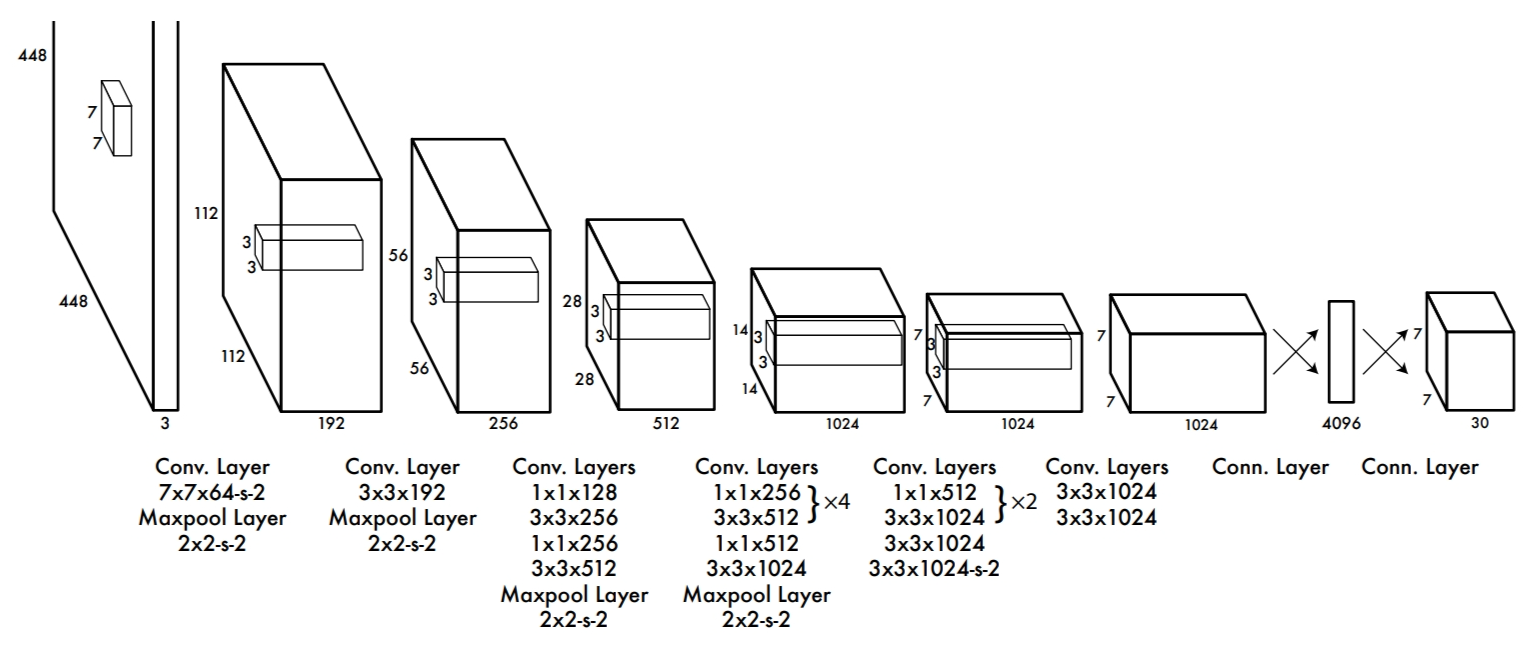
\includegraphics[scale=0.2]{resources/YOLO.png}
  \end{center}
  \caption[YOLO Architecture]{You Only Look Once Architecture}
  \label{fig:yolo architecture}
\end{figure}


\section{Object Relational Mapping (ORM)}
Object-Relational Mapping \cite{orm} เป็นการสร้างการสัมพันธ์ระหว่างฐานข้อมูลแบบ Relational กับโครงสร้างข้อมูลแบบ Object-Oriented 
ตามรูปที่ 2.2 ในการพัฒนาซอฟต์แวร์ เช่น เว็บแอปพลิเคชัน โดยที่ไม่ต้องเขียน SQL โดยตรงแต่สามารถใช้ภาษาโปรแกรมเพื่อจัดการกับข้อมูลแทน 
ซึ่งสามารถป้องกันการโจมตีแบบ SQL Injection ได้ ในกรณีที่กำหนดให้มีการเปลี่ยนแปลงในโครงสร้างข้อมูล 
คุณสมบัติหรือโครงสร้างข้อมูลในฐานข้อมูลจะถูกปรับเปลี่ยนตามในโครงสร้างของ Object ในโปรแกรม เป็นฐานข้อมูลแบบเสมือนในโปรแกรม 
โดยที่การจัดเก็บข้อมูลยังคงเป็นแบบ Relational เหมือนเดิม โดยไม่ต้องใช้ SQL Statements โดยตรง
\begin{figure}[ht]
  \begin{center}
  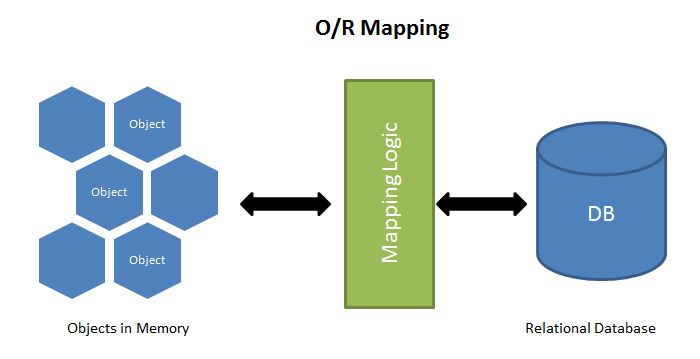
\includegraphics[scale=0.3]{resources/ORM.png}
  \end{center}
  \caption[Object Relational Mapping]{Object Relational Mapping}
  \label{fig:orm}
\end{figure}

\section{Model–View–Controller design pattern (MVC)}
Model-View-Controller \cite{mvc} เป็นรูปแบบโครงสร้างที่แยกแอปพลิเคชันออกเป็น 3 ส่วนหลักคือ: โมเดล (model), มุมมอง (view), 
และคอนโทรลเลอร์ (controller) แต่ละส่วนมีการสร้างขึ้นเพื่อจัดการด้านพัฒนาส่วนแอปพลิเคชันที่เฉพาะเจาะจง ตามรูปที่ 2.3 MVC 
เป็นหนึ่งในรูปแบบการพัฒนาเว็บตามมาตรฐานอุตสาหกรรมที่ถูกใช้บ่อยที่สุดเพื่อสร้างโครงงานที่สามารถเพิ่มและขยายขนาดในอนาคตได้ 
โดยที่ว่าเพื่อให้โปรแกรมนั้นดูเรียบง่ายต่อการแก้ไขจัดการ ซึ่งความหมายในแต่ละส่วนของ MVC นั้นได้แก่ 
\begin{enumerate}
  \item Model คือส่วนที่รับผิดชอบเกี่ยวกับข้อมูลและการประมวลผลทางด้านข้อมูลในแอปพลิเคชัน เช่น การเชื่อมต่อกับฐานข้อมูล การจัดการข้อมูล 
  และการประมวลผลทางข้อมูล เป็นต้น โดยที่ model มักจะเป็นตัวแทนของข้อมูลและสถานะของแอปพลิเคชัน
  \item View คือส่วนที่จะเป็นหน้าตาของโปรแกรมที่ผู้ใช้จะใช้งานจากส่วนนี้ ไม่ว่าจะเป็นการกรอกข้อมูล, ดูผลลัพธ์ หรือการมีปฏิสัมพันธ์กับผู้ใช้ 
  (User Interface) view จริง ๆ แล้วก็คือส่วนที่เรียกว่า GUI (Graphic User Interface) 
  \item Controller เป็นส่วนที่รับผิดชอบในการควบคุมและจัดการกับการกระทำที่เกิดขึ้นจากผู้ใช้งาน เช่น การรับข้อมูลจากผู้ใช้งาน, 
  การส่งข้อมูลไปยังโมเดลเพื่อประมวลผล, และการอัพเดตสถานะของ view ซึ่งโดยทั่วไปแล้ว controller จะเป็นตัวกลางที่เชื่อมต่อระหว่าง model 
  และ view โดยการควบคุมการทำงานของทั้งสอง 
\end{enumerate}
\begin{figure}[ht]
  \begin{center}
  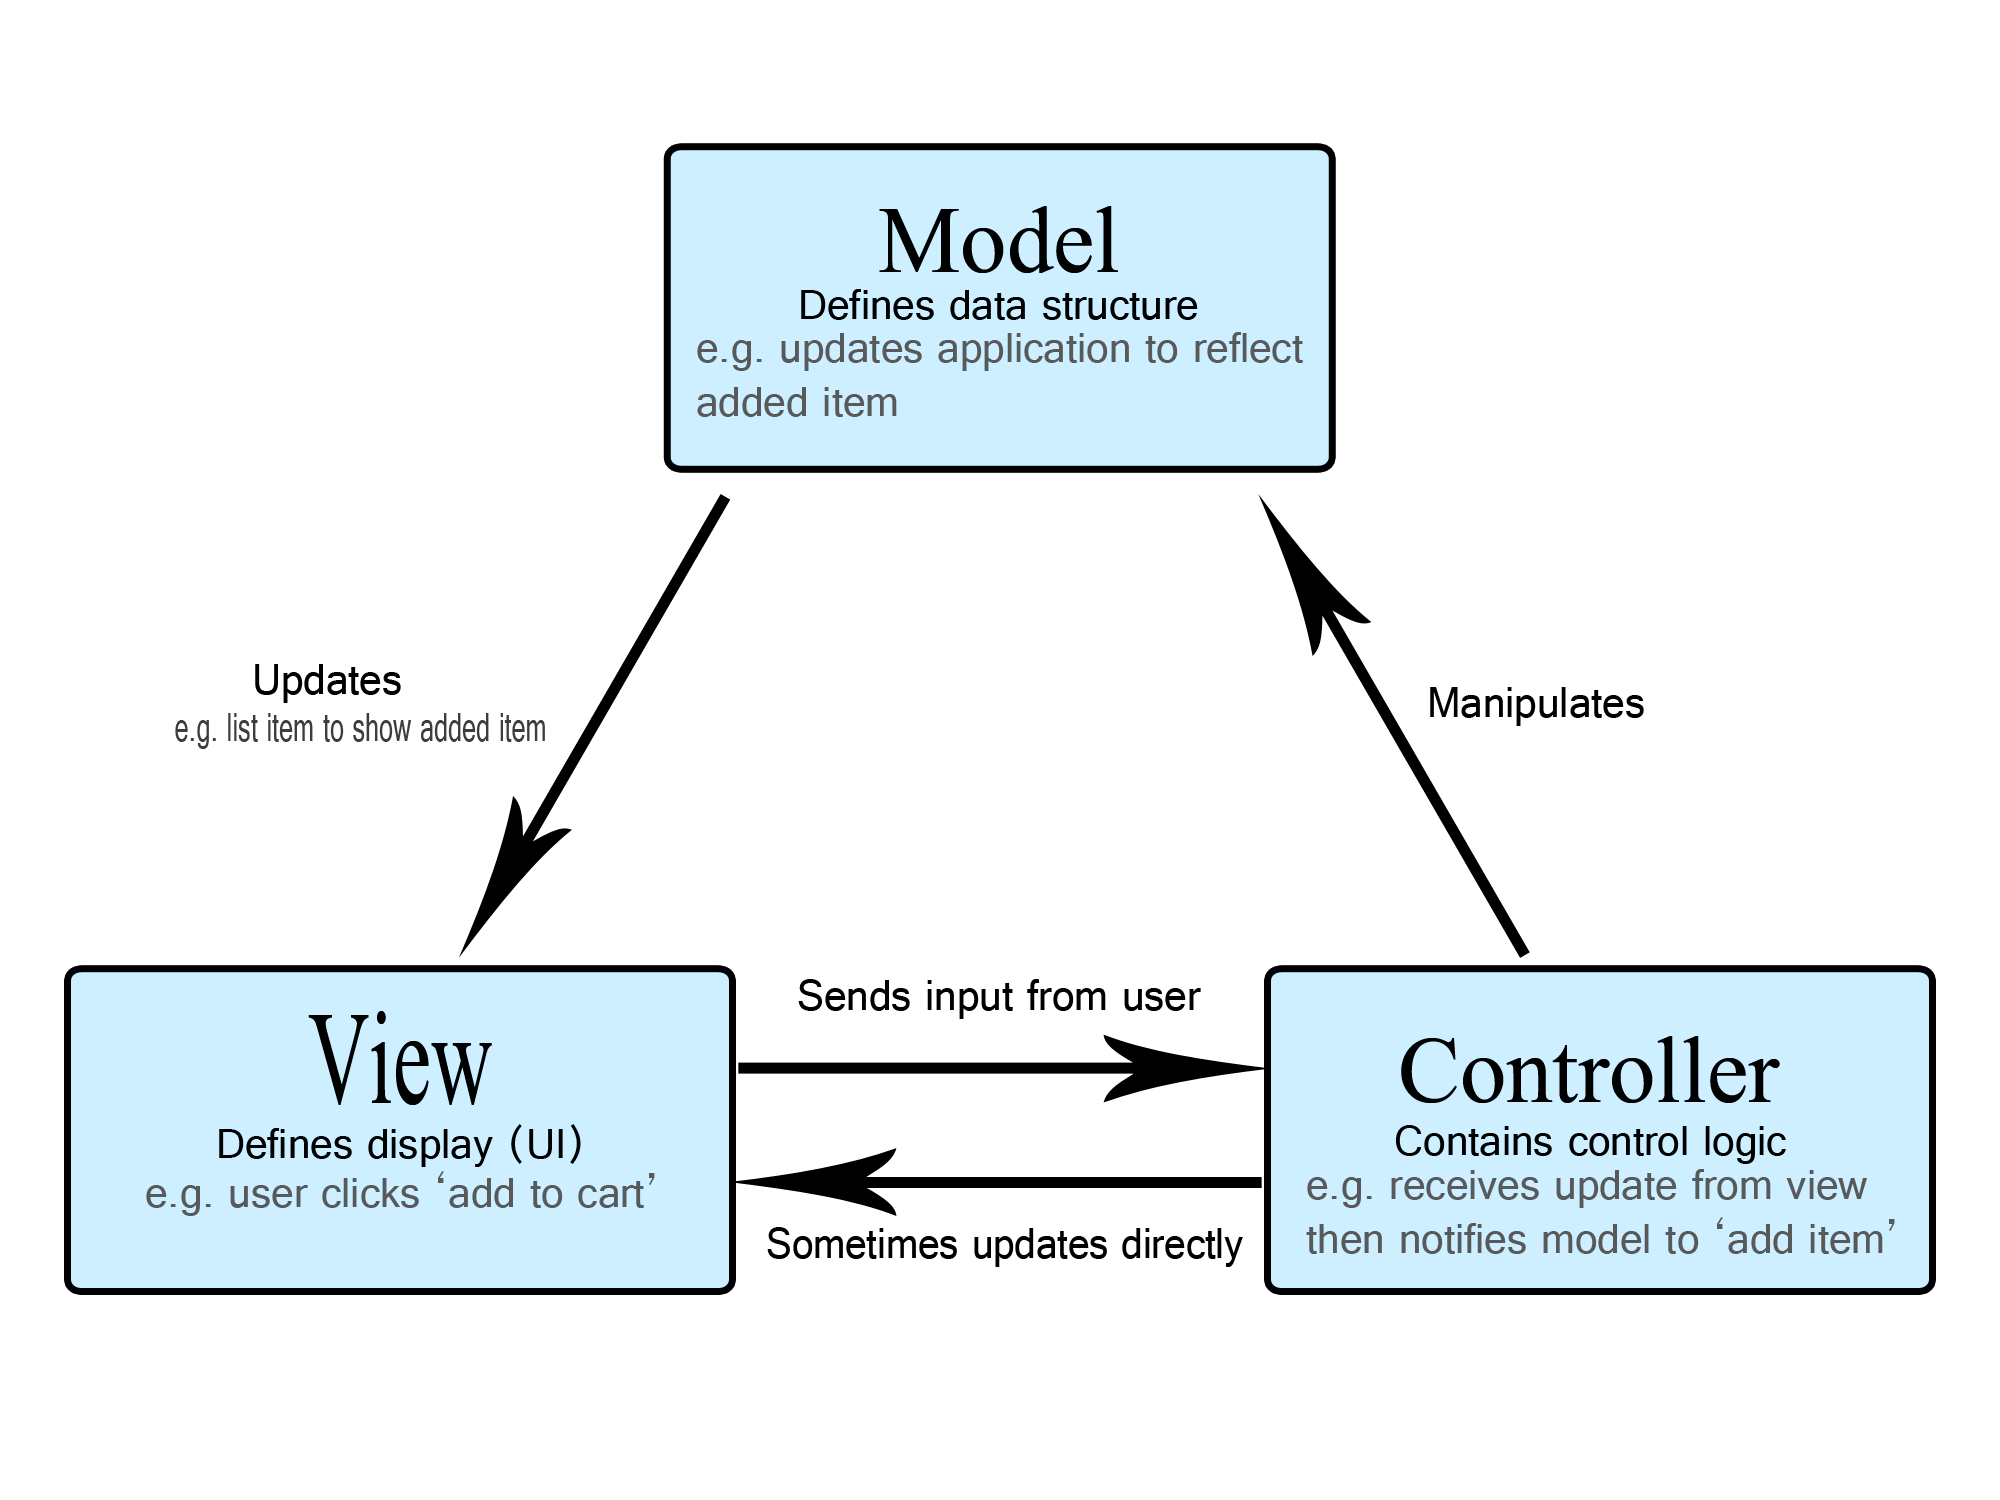
\includegraphics[scale=0.3]{resources/MVC.png}
  \end{center}
  \caption[Model-View-Controller]{Model-View-Controller Design Pattern}
  \label{fig:mvc}
\end{figure}

\section{Hypertext Transfer Protocol (HTTP)}
HTTP (Hypertext Transfer Protocol) เป็นโปรโตคอลสื่อสารที่ใช้ในการส่งข้อมูลระหว่างเครื่องคอมพิวเตอร์บนเครือข่ายอินเทอร์เน็ต โดย HTTP 
มีหน้าที่เป็นตัวกลางในการร้องขอและส่งข้อมูลระหว่างเว็บไซต์ (web servers) และเบราว์เซอร์ (web browsers) หรือแอปพลิเคชันอื่น ๆ 
ที่ใช้เครือข่ายอินเทอร์เน็ต 
\begin{itemize}
  \item API (Application Programming Interface) เป็นชุดของกฎและโครงสร้างข้อมูลที่กำหนดโดยโปรแกรมคอมพิวเตอร์เพื่อให้แอปพลิเคชันอื่น ๆ 
  สามารถสื่อสารและทำงานร่วมกันได้ ในเชิงพื้นฐาน API เป็นวิธีที่แอปพลิเคชันใช้เรียกใช้ฟังก์ชันหรือการบริการที่ให้มาจากแหล่งข้อมูลหรือบริการ
  ซึ่งอาจเป็นเซิร์ฟเวอร์เว็บ ฐานข้อมูล หรือแหล่งข้อมูลอื่น ๆ โดยทั่วไป API จะรองรับการร้องขอและการตอบกลับโดยใช้ฟอแมตที่เป็นรูปแบบมาตรฐาน เช่น 
  JSON (JavaScript Object Notation) หรือ XML (Extensible Markup Language) 
\end{itemize}

\section{Docker}
Docker \cite{docker} เป็นเทคโนโลยีคอนเทนเนอร์แพลตฟอร์มที่ช่วยในการสร้างและทำการงานร่วมกับคอนเทนเนอร์อย่างมีประสิทธิภาพ ด้วย Docker 
ผู้ใช้สามารถแยกแยะและแพคเกจแอปพลิเคชันพร้อมกับสิ่งที่เกี่ยวข้องทั้งหมด เช่น ไฟล์ ระบบปฏิบัติการ ไลบรารี และสิ่งอื่น ๆ 
ลงในคอนเทนเนอร์ได้อย่างเรียบง่าย โดยมีโครงสร้างการทำงานตามรูปที่ 2.4 ผู้ใช้สามารถสร้าง และรันคอนเทนเนอร์ได้โดยง่าย นอกจากนี้ Docker 
ยังช่วยลดปัญหาเกี่ยวกับสภาพแวดล้อมและการติดตั้งโปรแกรมที่ซับซ้อน ทำให้การพัฒนาและการทำงานของโปรแกรมมีประสิทธิภาพมากขึ้น 
\begin{figure}[ht]
  \begin{center}
  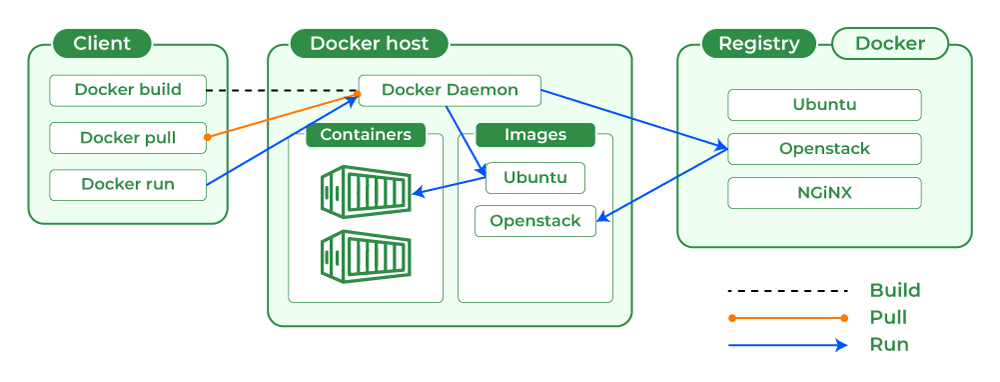
\includegraphics[scale=0.3]{resources/Docker.png}
  \end{center}
  \caption[Docker Architecture]{Docker Architecture}
  \label{fig:docker}
\end{figure}

\section{Interactive Website}
Interactive website \cite{interactive-web} คือ เว็บไซต์ที่สามารถให้ผู้ใช้งาน communicate หรือ interact เช่น การแสดงความคิดเห็น การตอบโต้กับตัวเว็บ 
การได้รับผลจากการกระทําในเว็บ ในลักษระที่เป็นมิตรต่อผู้ใช้ โดยปัจจุบัน มักใช้ animation sound picture audio etc. ประกอบ 
เพื่อให้มีความสนุกสนานและเพิ่มการเข้าถึงได้ง่ายของผู้ใช้ ทั้งนี้อาจทําเพื่อเก็บข้อมูลหลังจากการใช้งานเว็บไซต์ได้อีกด้วย ซึ่งดีกว่าเว็บที่มีแต่ตัวอักษร หรือ 
การแสดงผลเฉย ๆ ที่ได้รับข้อมูลทางฝ่ายเดียวอย่างแน่นอน

% \subsubsection{Subsubsection 1 heading goes here}
% Subsubsection 1 text

% \subsubsection{Subsubsection 2 heading goes here}
% Subsubsection 2 text

% \section{Third section}
% Section 3 text. The dielectric constant\index{dielectric constant}
% at the air-metal interface determines
% the resonance shift\index{resonance shift} as absorption or capture occurs
% is shown in Equation~\eqref{eq:dielectric}:

% \begin{equation}\label{eq:dielectric}
% k_1=\frac{\omega}{c({1/\varepsilon_m + 1/\varepsilon_i})^{1/2}}=k_2=\frac{\omega
% \sin(\theta)\varepsilon_\mathit{air}^{1/2}}{c}
% \end{equation}

% \noindent
% where $\omega$ is the frequency of the plasmon, $c$ is the speed of
% light, $\varepsilon_m$ is the dielectric constant of the metal,
% $\varepsilon_i$ is the dielectric constant of neighboring insulator,
% and $\varepsilon_\mathit{air}$ is the dielectric constant of air.

% \section{About using figures in your report}

% % define a command that produces some filler text, the lorem ipsum.
% \newcommand{\loremipsum}{
%   \textit{Lorem ipsum dolor sit amet, consectetur adipisicing elit, sed do
%   eiusmod tempor incididunt ut labore et dolore magna aliqua. Ut enim ad
%   minim veniam, quis nostrud exercitation ullamco laboris nisi ut
%   aliquip ex ea commodo consequat. Duis aute irure dolor in
%   reprehenderit in voluptate velit esse cillum dolore eu fugiat nulla
%   pariatur. Excepteur sint occaecat cupidatat non proident, sunt in
%   culpa qui officia deserunt mollit anim id est laborum.}\par}

% \begin{figure}[h]
%   \centering

%   \fbox{
%      \parbox{.6\textwidth}{\loremipsum}
%   }

%   % To include an image in the figure, say myimage.pdf, you could use
%   % the following code. Look up the documentation for the package
%   % graphicx for more information.
%   % \includegraphics[width=\textwidth]{myimage}

%   \caption[Sample figure]{This figure is a sample containing \gls{lorem ipsum},
%   showing you how you can include figures and glossary in your report.
%   You can specify a shorter caption that will appear in the List of Figures.}
%   \label{fig:sample-figure}
% \end{figure}

% Using \verb.\label. and \verb.\ref. commands allows us to refer to
% figures easily. If we can refer to Figures
% \ref{fig:walrus} and \ref{fig:sample-figure} by name in the {\LaTeX}
% source code, then we will not need to update the code that refers to it
% even if the placement or ordering of the figures changes.

% \loremipsum\loremipsum

% % This code demonstrates how to get a landscape table or figure. It
% % uses the package lscape to turn everything but the page number into
% % landscape orientation. Everything should be included within an
% % \afterpage{ .... } to avoid causing a page break too early.
% \afterpage{
%   \begin{landscape}
%   \begin{table}
%     \caption{Sample landscape table}
%     \label{tab:sample-table}

%     \centering

%     \begin{tabular}{c||c|c}
%         Year & A & B \\
%         \hline\hline
%         1989 & 12 & 23 \\
%         1990 & 4 & 9 \\
%         1991 & 3 & 6 \\
%     \end{tabular}
%   \end{table}
%   \end{landscape}
% }

% \loremipsum\loremipsum\loremipsum

% \section{Overfull hbox}

% When the \verb.semifinal. option is passed to the \verb.cpecmu. document class,
% any line that is longer than the line width, i.e., an overfull hbox, will be
% highlighted with a black solid rule:
% \begin{center}
% \begin{minipage}{2em}
% juxtaposition
% \end{minipage}
% \end{center}

% \section{\ifenglish%
% \ifcpe CPE \else ISNE \fi knowledge used, applied, or integrated in this project
% \else%
% ความรู้ตามหลักสูตรซึ่งถูกนำมาใช้หรือบูรณาการในโครงงาน
% \fi
% }

% อธิบายถึงความรู้ และแนวทางการนำความรู้ต่างๆ ที่ได้เรียนตามหลักสูตร ซึ่งถูกนำมาใช้ในโครงงาน

% \section{\ifenglish%
% Extracurricular knowledge used, applied, or integrated in this project
% \else%
% ความรู้นอกหลักสูตรซึ่งถูกนำมาใช้หรือบูรณาการในโครงงาน
% \fi
% }

% อธิบายถึงความรู้ต่างๆ ที่เรียนรู้ด้วยตนเอง และแนวทางการนำความรู้เหล่านั้นมาใช้ในโครงงาน

\chapter{\ifproject%
\ifenglish Project Structure and Methodology\else โครงสร้างและขั้นตอนการทำงาน\fi
\else%
\ifenglish Project Structure\else โครงสร้างของโครงงาน\fi
\fi
}

\makeatletter

% \renewcommand\section{\@startsection {section}{1}{\z@}%
%                                    {13.5ex \@plus -1ex \@minus -.2ex}%
%                                    {2.3ex \@plus.2ex}%
%                                    {\normalfont\large\bfseries}}

\makeatother
%\vspace{2ex}
% \titleformat{\section}{\normalfont\bfseries}{\thesection}{1em}{}
% \titlespacing*{\section}{0pt}{10ex}{0pt}

\section{การใช้งานพื้นฐาน}
ในส่วนของโมไบล์แอปพลิเคชัน เป็นเครื่องมือที่จะจำเป็นต้องใช้งานกล้องและบันทึกพิกัดตำแหน่งทาง GPS อยู่ตลอดเวลาเพื่อทำการส่งรูปภาพ 
พร้อมกับพิกัดตำแหน่ง แล้วนำไประมวลผลในเซอร์วิสที่ได้ออกแบบเอาไว้ โดยที่เซอร์วิสดังกล่าวจะทำการประมวลผลรูปภาพเพื่อหาป้ายโฆษณาที่สามารถจัดเก็บภาษีได้ 
และหลังจากนั้นก็จะจัดเก็บลงฐานข้อมูลต่อไป 

ในส่วนของเว็บแอปพลิเคชัน จะเป็นส่วนของการแสดงผลข้อมูลที่ได้บันทึกมาได้ส่วนของโมไบล์แอปพลิเคชัน โดยจะแสดงในรูปแบบของหมุดในแผนที่ 
คล้าย ๆ กับการปักหมุดของ Google map โดยที่ในแต่ละหมุดสามารถกดเพื่อดูรายละเอียดต่าง ๆ ได้ เช่น พิกัดของหมุดนั้น 
และลักษณะรูปป้ายในตำแหน่งนั้นๆที่ได้บันทีกมาจากโมไบล์แอปฯ 

\section{การออกแบบระบบพื้นฐานของโครงงาน}
\subsection{Database Design}
ประกอบด้วย 4 ตารางดังรูปที่ 3.1 ได้แก่
\begin{enumerate}
  \item User table: เนื่องจากระบบต้องมีการ Authentication เพื่อเข้าใช้งานไม่ว่าจะเป็นทั้งส่วนของ โมไบล์แอปฯ หรือเว็บแอปฯ 
  ดังนั้นตารางนี้จึงจะใช้เก็บข้อมูลพืื้นฐานต่าง ๆ ที่จำเป็นต่อการยืนยันตัวตนทั้งหมด 
  \item Role table: ใช้ในการเก็บบทบาททั้งหมดที่มีของระบบ เช่น ผู้ดูแลระบบ ผู้สำรวจ และอื่น ๆ 
  \item Asset table: ใช้ในการเก็บข้อมูลที่ได้รับมาจาก โมไบล์แอปฯ ไม่ว่าจะเป็นตำแหน่งของรูป ชื่อของรูป และประเภทของ asset ที่ตรวจจับได้ 
  \item Asset type table: ใช้ในการเก็บประเภทของ asset ต่างๆที่ระบบสามารถตรวจจับได้ 
  \item Config table: ใช้เก็บการตั้งค่าพื้นฐานต่างๆเช่น ขอบเขตของแผนที่ 
\end{enumerate}

\begin{figure}[ht]
  \begin{center}
  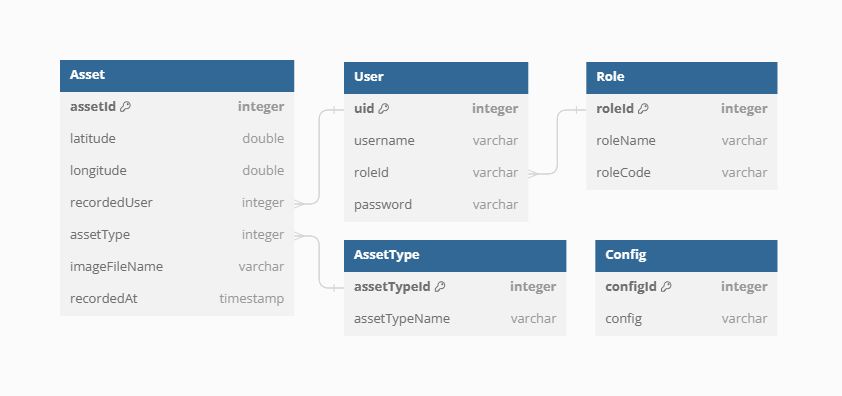
\includegraphics[scale=0.8]{resources/ScreetnerDB.png}
  \end{center}
  \caption[Database Design]{Overall Database Design}
  \label{fig:database}
\end{figure}

% TODO: DELETE IF NECESSARY
\newpage
\subsection{System Design}
จากรูป จะอธิบายถึงโครงสร้างระบบของโครงงานงานนี้ในรูปแบบ Flow diagram เพื่อให้เข้าใจถึงโครงสร้างการทำงานพอสังเขป 
โดยที่ซอฟต์แวร์จะประกอบด้วย 3 ส่วนหลัก ๆ ได้ Mobile application ซึ่งจะทำงานตามรูปที่ 3.2 Web application ซึ่งจะทำงานตามรูปที่ 3.3 
และ Processing server โดยที่ลักษณะการทำงานร่วมกันระหว่างทั้งสามส่วนประกอบ แสดงตามรูปที่ 3.1 

\begin{figure}[ht]
  \begin{center}
  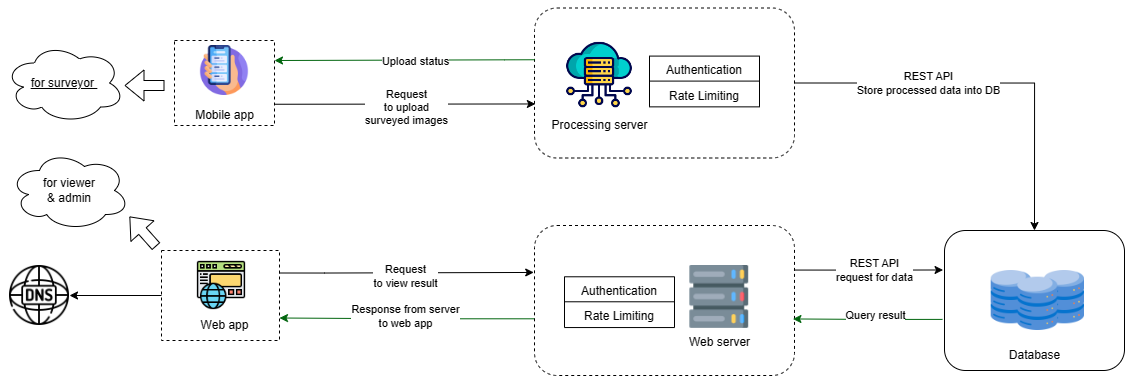
\includegraphics[scale=0.45]{resources/SystemDesign.png}
  \end{center}
  \caption[System Design]{Overall System Design}
  \label{fig:system design}
\end{figure}

% TODO: DELETE IF NECESSARY
\newpage
\subsection{Web Application Flow Diagram}
จากรูปที่ 3.3 จะอธิบายถึงลำดับการทำงานของเว็บแอปพลิเคชันในรูปแบบของ flow diagram เพื่อให้เข้าใจในลำดับการทำงานอย่างพอสังเขป 
พอหลังจากที่ได้เข้าระบบสู้หน้า dashboard จะมีตัวเลือกที่สามารถทำทำได้อยู่ 3 อย่างคือ filter เป็นการคัดกรองข้อมูลให้เหลือเพียงข้อมูลในช่วงเวลาที่เราต้องการ 
asset เป็นการกดที่รูปภาพเพื่อที่จะดูข้อมูลที่เกี่ยวกับ asset ดังกล่าว และ icon เป็นส่วนที่จะแสดงตัวเลือกเพิ่มเติมอีก 4 ทางเพื่อให้เราสามารถเลือกเข้าไปยังหน้าอื่นต่อไปได้

\begin{figure}[ht]
  \begin{center}
  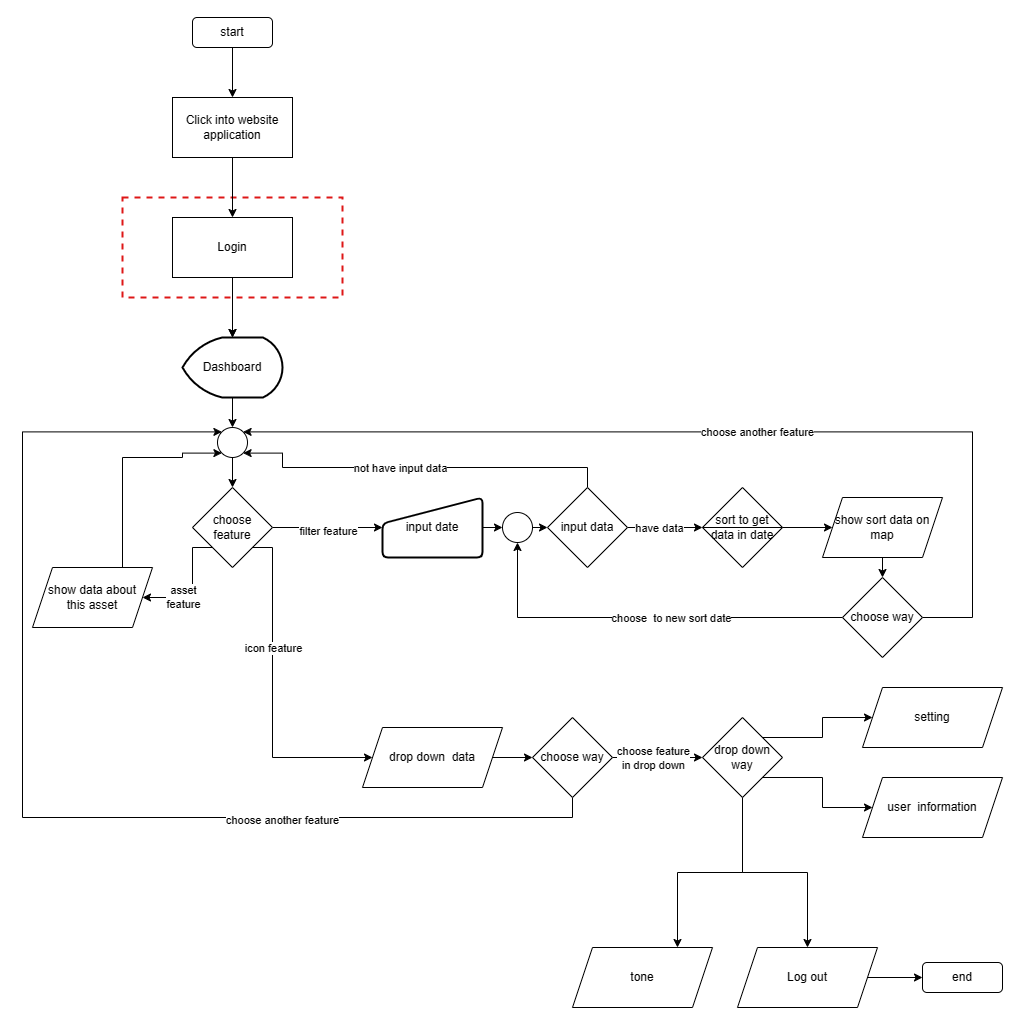
\includegraphics[scale=0.65]{resources/WebsiteFlow.png}
  \end{center}
  \caption[Web Application Flow Diagram]{Web Application Flow Diagram}
  \label{fig:web-app flow design}
\end{figure}

% TODO: DELETE IF NECESSARY
\newpage
\subsection{Mobile Application Flow Diagram}
รูปที่ 3.4 จะอธิบายถึงลำดับการทำงานขอโมไบล์แอปพลิเคชันในรูปแบบของ flow diagram เพื่อให้เข้าใจในลำดับการทำงานอย่างพอสังเขป โดยพอผู้ใช้จะเริ่มเข้าใช้งานแอปพลิเคชัน 
ผู้ใช้จะต้องผ่านการเข้าสู่ระบบ ซึ่งมีขั้นตอนการทำงานดังรูปที่ 3.5 เพื่อเป็นการยืนยันตัวตน หลังจากที่ได้เข้าสู่แอปพลิเคชันเรียบร้อยแล้ว 
ผู้ใช้งานจะสามารถเริ่มสตรีมวิดีโอเพื่อทำการส่งรูปภาพในช่วงเวลาหนึ่งพร้อมแนบตำแหน่งพิกัดในช่วงเวลาดังกล่าวไปยังเซอร์วิสที่ได้จัดเตรียมเอาไว้อยู่ตลอดเวลาที่ทำการสตรีม 
เพื่อให้ทางเซอร์วิสทำการคืนค่าออกมาว่าในตำแหน่งนี้จะมี asset อยู่เท่าไหร่ โดยจะมีขั้นตอนการทำงานดังรูปที่ 3.6 
ซึ่งสิ่งที่คืนค่ามาทุกครั้งนั้นจะเอามาจัดเก็บเอาไว้บนมือถือชั่วคราวและยังไม่ได้ทำการบันทึกข้อมูลลงไปในฐานข้อมูลเพื่อให้ผู้ใช้งานสามารถดูข้อมูลได้ตลอดเวลาว่าปัจจุบันมี 
asset อยู่เท่าไหร่จนจบการทำงาน และในตอนท้ายของการทำงานผู้ใช้สามารถที่จะเลือกได้ว่าจะทำการสตรีมต่ออีกครั้งหรือไม่ หากไม่ทำการสตรีมต่อ 
ผู้ใช้งานต้องเลือกว่าจะทำการส่งข้อมูลทั้งหมดที่ได้มานั้นไปยังฐานข้อมูลหรือไม่
\begin{figure}[ht]
  \begin{center}
  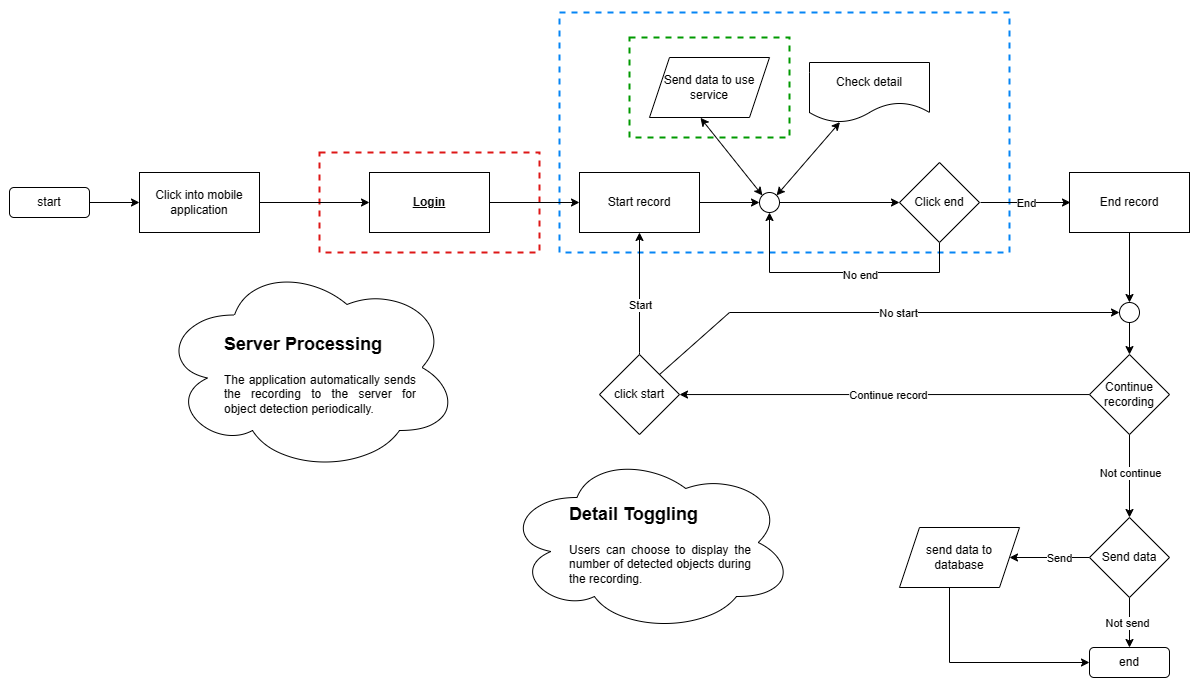
\includegraphics[scale=0.5]{resources/MobileAppFlow.png}
  \end{center}
  \caption[Mobile Application Flow Diagram]{Mobile Application Flow Diagram}
  \label{fig:mopile-app flow design}
\end{figure}

\begin{figure}[ht]
  \begin{center}
  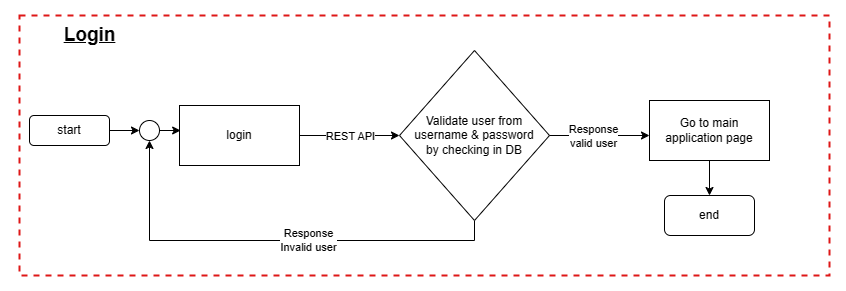
\includegraphics[scale=0.6]{resources/LoginFlow.png}
  \end{center}
  \caption[Login Flow Diagram]{Login Flow Diagram}
  \label{fig:login flow design}
\end{figure}

\begin{figure}[ht]
  \begin{center}
  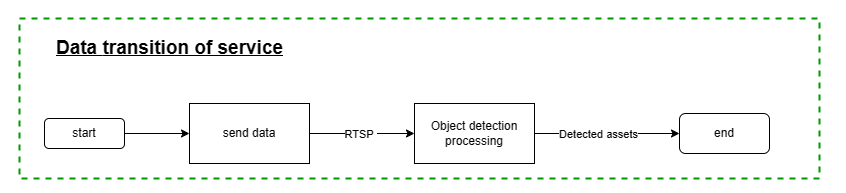
\includegraphics[scale=0.6]{resources/TransitionFlow.png}
  \end{center}
  \caption[Transition Flow Diagram]{Transition Flow Diagram}
  \label{fig:transition flow design}
\end{figure}

\chapter{\ifenglish General Company Information\else ข้อมูลทั่วไปของบริษัท\fi}

\section{\ifenglish Company Products and Services\else สินค้าและบริการของบริษัท \fi}
บริษัท เอสซีบี เทคเอกซ์ มีความเชี่ยวชาญในการพัฒนานวัตกรรมและเทคโนโลยีที่สามารถตอบสนองความต้องการของลูกค้าในด้านการบริการอย่างครบวงจร โดยนำเสนอบริการที่หลากหลายซึ่งครอบคลุมตั้งแต่การให้คำปรึกษาไปจนถึงการพัฒนาโซลูชันทางเทคโนโลยี รวมถึงการวิเคราะห์ความต้องการของระบบ การออกแบบ การพัฒนาซอฟต์แวร์จนถึงการใช้งานจริง นอกจากนี้ บริษัทยังให้บริการด้านโครงสร้างพื้นฐานเทคโนโลยีและการประมวลผลบนระบบคลาวด์เพื่อสนับสนุนการดำเนินงานในยุคดิจิทัล

เพื่อสนับสนุนการตัดสินใจเชิงธุรกิจ บริษัทได้พัฒนาบริการจัดการข้อมูลที่สามารถสร้างข้อมูลเชิงลึกให้กับลูกค้า พร้อมทั้งมีบริการด้านความปลอดภัยทางไซเบอร์เพื่อปกป้องข้อมูลและระบบการดำเนินงานในสภาพแวดล้อมดิจิทัล


\begin{enumerate}
  \item eKYC (Electronic Know Your Customer) เป็นซอฟต์แวร์ที่พัฒนาขึ้นตามพระราชบัญญัติป้องกันและปราบปรามการฟอกเงิน ซึ่งกำหนดให้ธุรกิจที่เกี่ยวข้องกับการเงินและการลงทุนต้องดำเนินการระบบ KYC (Know Your Customer) ก่อนทำธุรกรรม ในอดีต การยืนยันตัวตนผู้ใช้บริการจะต้องใช้วิธีการกรอกเอกสาร ซึ่งอาจทำให้กระบวนการช้าและซับซ้อน เพื่อเพิ่มความสะดวกและความรวดเร็วในการยืนยันตัวตน บริษัทจึงได้สร้างซอฟต์แวร์นี้ขึ้น โดยนำเทคโนโลยีการสแกนใบหน้าและบัตรประชาชนมาใช้ ซึ่งช่วยให้กระบวนการยืนยันตัวตนสามารถดำเนินการได้อย่างรวดเร็ว
  \item xPlatform ได้นำแนวทางปฏิบัติที่มีประสิทธิภาพใน DevOps มาประยุกต์ใช้ในการออกแบบแพลตฟอร์มอัตโนมัติ  ในรูปแบบ Web Application ซึ่งช่วยให้ลดภาระการทำงานของทั้งทีมพัฒนาและทีมปฏิบัติการ โดยที่แพลตฟอร์มนี้มีฟีเจอร์ที่รองรับทุกขั้นตอนของวงจรซอฟต์แวร์ ตั้งแต่การพัฒนา การทดสอบ การปล่อยซอฟต์แวร์ ไปจนถึงการบำรุงรักษา การเฝ้าระวัง และการเพิ่มประสิทธิภาพ นอกจากนี้ยังช่วยสนับสนุนการทำงานร่วมกันแบบ Agile บนแพลตฟอร์มเดียว ซึ่งฟีเจอร์เหล่านี้ยังช่วยให้ PO/PM สามารถบริหารทีมและควบคุมงบประมาณของโครงการเพื่อลดค่าใช้จ่ายที่ไม่จำเป็น
  \item TechX Data Platform เป็นแพลตฟอร์มที่ออกแบบมาเพื่อให้การจัดการข้อมูลเป็นเรื่องง่ายและครบวงจร โดยครอบคลุมทุกขั้นตอน ตั้งแต่การนำเข้าข้อมูล การจัดเก็บ การจัดการ การวิเคราะห์ จนถึงการรักษาความปลอดภัยของข้อมูล นอกจากนี้ยังมีบริการวิเคราะห์ข้อมูลขั้นสูงด้วยเทคโนโลยี Machine Learning ที่สามารถปรับแต่งให้เหมาะสมกับธุรกิจได้ทุกรูปแบบ ไม่ว่าจะเป็น Startup ธุรกิจ SME หรือองค์กรขนาดใหญ่ ซึ่งมีความต้องการด้านข้อมูลที่แตกต่างกันไป
  \item บริษัทมีบริการให้คำปรึกษาและพัฒนาโซลูชันครบวงจร เพื่อตอบสนองความต้องการของลูกค้าและผู้มีส่วนเกี่ยวข้อง โดยใช้เฟรมเวิร์คกระบวนการคิดเชิงออกแบบ (Design Thinking) นอกจากนี้ บริษัทยังมีทีมวิศวกรซอฟต์แวร์และนักออกแบบประสบการณ์ผู้ใช้ (UX Designer) ที่มีความเชี่ยวชาญในการพัฒนาโซลูชันให้กลายเป็นผลิตภัณฑ์จริง
  \item บริการโซลูชันด้านคลาวด์ที่เน้นความยืดหยุ่นและประสิทธิภาพในการจัดการโครงสร้างพื้นฐานทางไอที รวมถึงการย้ายข้อมูลและการรักษาความปลอดภัยบนคลาวด์ บริการเหล่านี้ครอบคลุมตั้งแต่การออกแบบสถาปัตยกรรมระบบ การจัดการทรัพยากรไอที จนถึงการเฝ้าระวังและปรับปรุงประสิทธิภาพของระบบ ทีมงานยังมีความเชี่ยวชาญในการบริหารจัดการระบบคลาวด์หลากหลายแพลตฟอร์ม (multi-cloud) และใช้กระบวนการที่เน้นความปลอดภัยในทุกขั้นตอน
\end{enumerate}

\renewcommand{\arraystretch}{1.2}
\newcommand{\attr}[1]{\hspace{2pt}#1\hspace{2pt}}
\section{งบแสดงฐานะการเงิน}
\begin{table}[H]
  \centering
  \begin{tabular}{c||c|c|c}
      \multirow{2}{*}{ปี} & \multicolumn{3}{c}{จำนวน (ล้านบาท)} \\
      \cline{2-4}
       & \attr{สินทรัพย์} & \attr{หนี้สิน} & \attr{ส่วนผู้ถือหุ้น} \\
      \hline\hline
      2021 & 1742 & 1241 & 501 \\
      2022 & 2351 & 821  & 1529\\
      2023 & 1954 & 587  & 1367\\
  \end{tabular}
  \caption{โครงสร้างงบฐานะการเงินปี 2021 ถึงปี 2023}
  \label{tab:company-asset-table-1}
\end{table}
\begin{table}[H]
  \centering
  \begin{tabular}{c||c|c|c}
       ปี & \attr{สินทรัพย์} & \attr{หนี้สิน} & \attr{ส่วนผู้ถือหุ้น} \\
      \hline\hline
      2021 & 0 & 0  & 0 \\
      2022 & 0.35 & -0.34  & 2.05\\
      2023 & -0.11 & -0.29  & -0.17\\
  \end{tabular}
  \caption{อัตราการเปลี่ยนแปลงโครงสร้างงบฐานะการเงินปี 2021 ถึงปี 2023}
  \label{tab:company-asset-table-2}
\end{table}
บริษัท เอสซีบี เทคเอกซ์ ซึ่งเป็นบริษัทในเครือของธนาคารไทยพาณิชย์ มีสินทรัพย์ที่สูงมากสำหรับบริษัทใหม่ โดยในปีแรก (2021) บริษัทมีสินทรัพย์รวม 1742 ล้านบาท จากนั้นสินทรัพย์เพิ่มขึ้นเป็น 2351 ล้านบาทในปี 2022 ในปีนี้ ส่วนของผู้ถือหุ้นเพิ่มขึ้นกว่า 1000 ล้านบาท จาก 501 ล้านบาทในปี 2021 เป็น 1529 ล้านบาท แม้ในปี 2023 สินทรัพย์จะลดลงเล็กน้อยมาอยู่ที่ 1954 ล้านบาท แต่ส่วนของผู้ถือหุ้นยังคงสูงอยู่ที่ 1367 ล้านบาท

ในด้านหนี้สิน บริษัทเริ่มต้นด้วยหนี้สิน 1241 ล้านบาทในปี 2021 ทำให้อัตราส่วนหนี้สินต่อทุนอยู่ที่ 2.43 เท่า จากนั้นบริษัทปรับลดระดับหนี้สินอย่างต่อเนื่อง ในปี 2022 หนี้สินลดลงเหลือ 821 ล้านบาท และในปี 2023 ลดลงเหลือ 587 ล้านบาท ส่งผลให้อัตราส่วนหนี้สินต่อทุนในปี 2023 อยู่ที่ 0.49 เท่า

\section{งบกำไรขาดทุน}
\begin{table}[H]
  \centering
  \begin{tabular}{c||c|c|c|c}
      \multirow{2}{*}{ปี} & \multicolumn{4}{c}{จำนวน (ล้านบาท)} \\
      \cline{2-5}
       & \attr{กำไรสุทธิ} & \attr{กำไรก่อนภาษี} & \attr{รายจ่ายรวม} & \attr{รายได้รวม} \\
      \hline\hline
      2021 & 350 & 438 & 1158 & 1596\\
      2022 & 672 & 840  & 2329 & 3169\\
      2023 & 246 & 308  & 1978 & 2289\\ 
  \end{tabular}
  \caption{โครงสร้างงบกำไรขาดทุนปี 2021 ถึงปี 2023}
  \label{tab:company-asset-table-1}
\end{table}
\begin{table}[H]
  \centering
  \begin{tabular}{c||c|c|c|c}
       ปี & \attr{กำไรสุทธิ} & \attr{กำไรก่อนภาษี} & \attr{รายจ่ายรวม} & \attr{รายได้รวม} \\
      \hline\hline
      2021 & 0 & 0 & 0 & 0\\
      2022 & 0.92 & 0.92  & 1.01 & 0.99\\
      2023 & -0.63 & -0.63  & -0.15 & -0.28\\
  \end{tabular}
  \caption{อัตราการเปลี่ยนแปลงโครงสร้างงบกำไรขาดทุนปี 2021 ถึงปี 2023}
  \label{tab:company-asset-table-2}
\end{table}
ในปีแรกของบริษัท มีผลกำไรสุทธิอยู่ที่ 350 ล้านบาท ขณะที่รายได้รวมอยู่ที่ 1596 ล้านบาท ซึ่งแสดงให้เห็นว่าบริษัทมีอัตรากำไรสุทธิที่ 0.219 เท่า เมื่อเปรียบเทียบกับรายได้รวมในปีถัดมาในปี 2022 อัตราการเพิ่มของรายได้รวมและรายจ่ายรวมของบริษัทได้เพิ่มขึ้นเท่าตัว โดยรายจ่ายรวมอยู่ที่ 2329 ล้านบาท และรายได้รวมอยู่ที่ 3169 ล้านบาท ซึ่งอัตรากำไรสุทธิในปีนั้นอยู่ที่ 0.212 เท่า แสดงให้เห็นว่าบริษัทยังคงรักษาอัตรากำไรสุทธิในระดับที่ใกล้เคียงกับปีแรก

ในปีถัดมา มีการลดอัตรารายจ่ายรวมและรายได้รวม โดยอัตราการลดของรายได้รวมนั้นเกือบสองเท่าของอัตราการลดรายจ่ายรวม ทำให้รายจ่ายรวมลดลงเหลือ 1978 ล้านบาท และรายได้รวมอยู่ที่ 2289 ล้านบาท ผลลัพธ์นี้ทำให้อัตรากำไรสุทธิของบริษัทตกลงเหลือเพียง 0.107 เท่า ซึ่งแสดงให้เห็นว่าบริษัทมีการเติบโตในปีแรกและปีที่สอง แต่ในปีที่สามกลับมีแนวโน้มการลดลงของอัตรากำไรสุทธิ อาจบ่งบอกถึงความท้าทายที่บริษัทเผชิญหรือเกิดจากการตัดสินใจลดขนาดหนี้สิน
\chapter{\ifenglish Assigned Work and Terms of Reference\else งานที่รับมอบหมายและรางขอบเขตงาน\fi}
please extend this


\section{\ifenglish Terms of Reference for Cooperative Education\else รางขอบเขตงานกระบวนวิชาสหกิจศึกษา \fi}
Starting salary: 30k baht. Increase once a year, based on the employee's performace.

\section{\ifenglish Assigned Work\else งานที่ได้รับมอบหมาย \fi}
% TODO: lengthen this
งานที่ได้รับมอบหมาย โดยส่วนใหญ่แล้วจะเป็นงานที่ได้ทำงานกับทีม xPlatform ซึ่งเป็นโปรเจคใหญ่ของบริษัท เอสซีบี เทคเอกซ์ ด้วยเช่นกัน โดยงานที่ได้รับมอบหมายจะสามารถแบ่งออกได้เป็น 4 งานหลักดังนี้

\subsection{\ifenglish xPlatform Change Runbook​ Feature\else ฟีเจอร์ xPlatfrom Change Runbook\fi}
% TODO: clarify this
ในขั้นตอนของการพัฒนาซอฟต์แวร์นั้น ถ้าหากว่าผู้พัฒนานั้นจำเป็นต้องการไปปรับเปลี่ยน configuration ของระบบต่าง ๆ ที่เกี่ยวข้องนั้น ผู้พัฒนาการจะไม่สิทธิในการที่จะไปปรับเปลี่ยนส่วนนั้นได้โดยตรง อย่างเช่น ขั้นตอนการ deploy แต่ละส่วนของระบบรวม การปรับเปลี่ยนสิทธิการเข้าถึงข้อมูล ซึ่งการเปลี่ยนแปลงเหล่านี้จะต้องไปแจ้งพนักงานในแผนกอื่น ๆ ที่มีสิทธิในการเข้าถึงเท่านั้นอย่างเช่น อย่างเช่น DevOps IT แผนกผู้บริหารฐานข้อมูล 

การทำงานแต่ละขั้นตอน จะมีชื่อเรียกว่า Activity รายงานขั้นตอนของการทำงานที่จะแจ้งแผนกต่าง ๆ นั้นจะมีชื่อว่า Runbook โดยที่ขั้นตอนดังกล่าวนี้โดยปกติจะทำรวมกับการเปลี่ยนแปลงเวอร์ชั่นของซอฟต์แวร์ที่จะเรียกว่า Change หรือที่มักจักเป็นที่รู้จักกันว่า Release โดยปกติแล้ว การขั้นตอนการเขียน Runbook นั้นจะลงเองด้วยมือ ซึ่งเป็นเรื่องที่ค่อนข้างเสียเวลามาก และสามารถเกิดข้อผิดพลาดขณะการเขียนได้ง่าย เราจึงได้สร้างฟีเจอร์ Change Runbook เพื่อช่วยให้นักพัฒนาซอฟต์แวร์สามารถรายงานขั้นตอนการทำงานได้สะดวกขึ้น

\[\text{add a blurred change runbook image here}\]

โดยที่ฟีเจอร์นี้จะมีความต้องการดังนี้
\begin{enumerate}
    \item ในแต่ละ Change จะมีอยู่หนึ่ง Runbook โดยที่ แต่ละ Runbook จะมีอยู่หลาย ๆ กลุ่มงาน (Activity Groups) แล้วแต่ละ Activity Groups จะมีอยู่หลาย ๆ Activities ในแต่ละ Activity จะต้องประกอบไปด้วยข้อมูล 
    \begin{enumerate}
        \item ชื่อ (Title)
        \item รายละเอียด (Description) 
        \item แท็ก (Hashtag)
        \item ผู้ที่รับผิดชอบ (Owner) (แผนกหรือพนังงานที่มีส่วนเกี่ยวข้องในการทำงาน)
        \item เวลาเริ่มต้นและเวลาสิ้นสุดของการทำงานขั้นตอนนั้น ๆ (Impl-start กับ Impl-end)
        \item Activities ที่จะต้องถูกทำงานเสร็จก่อน (Dependency)
        \item ประเภทของ Activity (Deploy กับ Rollback)
        \item สถานะการทำงาน (กำลังดำเนินอยู่ สำเร็จ ล่าช้า 10 นาที ล่าช้า 20 นาที และ ล่าช้าจนมีผลกระทบ)
        \item ความก้าวหน้าของงาน (0\% 20\% 40\% 60\% 80\% และ 100\%)
    \end{enumerate}
    ซึ่งจะมีแผนผังแสดงความสัมพันธ์ระว่าง Entity ดังนี้
    \[\text{insert ER diagram here}\]
    \item ผู้ที่จะสามารถเปลี่ยนแปลงข้อมูล (Update) หรือลบ (Delete) Activity ได้ จะเป็นผู้ที่สร้าง Activity นั้น ๆ หรือ Product Manager กับ Product Owner (PO \& PM)
    \item ในแต่ละ Activity จะสามารถเปลี่ยนแปลงสถานะการทำงานหรือความก้าวหน้าของงานได้ ซึ่งการทำเช่นนี้จะมีเรียกว่าการ Marking โดยที่ผู้ที่จะสามารถ Mark ได้จะเป็นเพียงแค่ผู้ที่มีหน้าที่รับผิดชอบ (Responsible people) หรือผู้ใช้ที่มีหน้าที่เป็น PO \& PM ซึ่งผู้ Mark จะสามารถระบุโน้ต หรือว่า Issue ที่เกี่ยวข้องกับการเปลี่ยนแปลงนั้นได้
    \item ในแต่ละ Activity จะสามารถแบ่งวิธีการหนดเวลาได้เป็น 2 รูปแบบ ได้แก่ Absolute กับ Relative โดยที่ 
    \begin{enumerate}
        \item Absolute Activity คือ Activity ที่ในขณะที่ถูก Create หรือ Update นั้น ผู้ใช้งานจะต้องระบุเวลาเริ่มต้นและเวลาจบของงาน โดยที่เวลาเริ่มต้นของ Activity ดังกล่าวต้องมาหลังเวลาจบของทุก ๆ Dependency (Time Constraint)
        \item Relative Activity คือ Activity ที่ในขณะที่ถูก Create หรือ Update นั้น ผู้ใช้จะระบุเพียงแค่ระยะการทำงานของ Activity นั้น ๆ โดยที่เวลาเริ่มต้นกับเวลาจบนั้นจะขึ้นอยู่กับ Time Constraint กล่าวคือ เวลาเริ่มต้นของ Activity นั้น ๆ จะเท่ากับ Time Constraint เสมอ ซึ่งหมายความว่าทุก ๆ Relative Activity จะจำเป็นต้องมีอย่างน้อย 1 Dependency
    \end{enumerate}
    \item ในการ Update Activity นั้น อาจเกิดกรณีทีี Activity นั้นเป็น Dependency ของ Activity ตัวอื่น ๆ ได้ ซึ่งเวลาการทำงานของ Activity ดังกล่าวนั้นจะจำเป็นต้องเปลี่ยนไปอัตโนมัติตามกฎดังนี้
    \begin{enumerate}
        \item หาก Time Constraint ของ Absolute Activity ถูกเลื่อนไปอยู่หลัง Activity นั้น เวลาในการทำงานของ Activity จะถูกเลื่อนตามไปอยู่หลัง Time Constraint โดยผู้ใช้สามารถเลือกที่จะ Bypass Absolute Activity เพื่อไม่ให้เวลาการทำงานของ Activity เปลี่ยนแปลง แต่จะทำให้ความเป็น Dependency ของ Activities ที่เสร็จหลังก่อนที่ Absolute Activity จะเริ่ม นั้นถูกยกเลิก 
        \item Relative Activity จะต้องเปลี่ยนเวลาใหม่ถ้าหาก Time Constraint เปลี่ยน
    \end{enumerate}
    \[\text{add update example here}\]
    \item ในการ Delete Activity นั้น ถ้าหากตัวท่ีกำลังถูกลบอยู่เป็น Dependency ตัวเดียวของ Required Activity  Activity นั้นจะถูกโปรโมทให้เป็น Absolute Activity แทน
    \[\text{add delete example here}\]
    \item ผู้ใช้สามารถดึงข้อมูล (Import) จากไฟล์ประเภท CSV ได้ % TODO: complete this
    \item ผู้ใช้สามารถดึงข้อมูลของ Issues จากเว็บไซต์ Jira ในการสร้าง​ Activity ได้ โดยที่ผู้ใช้งานจะสามารถคัดเลือกข้อมูล (Query) ได้อยู่สองวิธี
    \begin{enumerate}
        \item การ Query แบบ Basic: ผู้ใช้จะต้องระบุ โค้ดของโปรเจค Label ของ Issue และ ประเภทของ Issue
        \item การ Query ด้วย Jira Query Lanauge (JQL) ซึ่งเป็นภาษาที่ช่วยในการค้นหาข้อมูลใด ๆ ก็ตามภายในเว็บไซต์ของ Jira
    \end{enumerate}
    โดยที่วิธีการดึงข้อมูลนี้จะแตกต่างกันตาม Type ของ Field ที่กำลังถูกดึง นอกจากนี้ Activity ที่ถูกดึงมา จะสามารถลิงก์กลับไปบนหน้่าเว็บเพจของ Issue นั้น ๆ บน Jira ได้ด้วยเช่นกัน
    \[\text{example jira issue}\]
    \item การ Import จากแหล่งใดก็ตามจะได้ประเภทการกำหนดเวลาแบบ Absolute เสมอ เนื่องจากการ Import จะไม่สามารถระบุ Dependency ได้ ผู้ใช้จะสามารถเพิ่ม Dependency ด้วยการ Update ทีหลัง
    \item ผู้ใช้การจะสามารถส่งออกข้อมูล (Export) ของ Runbook ออกเป็นไฟล์ .xlsx ได้

\end{enumerate}

\subsection{\ifenglish Fast Easy Tasks\else งานร่วมกับทีม fast easy\fi}

\subsection{\ifenglish Keycloak user credentail data synchronisation\else งานการบันทึก credential ของผู้ใช้ลงซอฟต์แวร์ Keycloak\fi}

\subsection{TBA}

% TODO: UNCOMMENT THE FOLLOWING
% \chapter{\ifproject%
% \ifenglish Experimentation and Results\else การทดลองและผลลัพธ์\fi
% \else%
% \ifenglish System Evaluation\else การประเมินระบบ\fi
% \fi}

% TODO: DELETE THE FOLLOWING
\chapter{\ifenglish System Evaluation\else การประเมินระบบ\fi}

\section{การประเมินประสิทธิภาพซอฟต์แวร์}
ทดสอบประสิทธิภาพซอฟต์แวร์โดยจะมีการแบ่งส่วนในการทดสอบออกเป็นส่วน ๆ เพื่อให้รู้ว่าในแต่ละส่วนของซอฟต์แวร์ของเรานั้น 
ทำงานได้อย่างมีประสิทธิภาพหรือไม่ จึงสามารถแบ่งออกการประเมินได้เป็นดังนี้ 
\begin{enumerate}
    \item Classification model - เป็นการทดสอบเพื่อประเมินและตรวจสอบความเร็วในการประมวลผลเพื่อทำการ classify 
    ว่า object ใดเป็นป้ายที่สามารถจัดเก็บภาษีได้ รวมถึงในเรื่องของความแม่นยำในการ classify  
    \item Response time - เป็นการทดสอบเพื่อประเมินในเรื่องของความเร็วในการรับส่งข้อมูลระหว่าง client กับ application server  
\end{enumerate}

\section{การประเมินความพึงพอใจในการใช้งานระบบ}
ทดสอบความพึงพอใจในการใช้งานจะมีการแบ่งออกเป็นสองส่วน คือส่วนของแอปพลิเคชันในโทรศัพท์มือถือ กับส่วนของเว็บแอปพลิเคชัน 
โดยจะมีเกณฑ์การให้คะแนนอยู่ที่ 1 ถึง 5 โดยจะมีการให้คะแนนในเรื่องดังต่อไปนี้ 
\begin{enumerate}
    \item ความง่ายต่อการใช้งานของแอปพลิเคชัน 
    \item ความสะดวกในการใช้งานในตอนเริ่มต้นของแอปพลิเคชัน 
    \item ความดึงดูดในการใช้งานของแอปพลิเคชัน        
    \item ประโยชน์ที่มีของแอปพลิเคชัน 
\end{enumerate}
โดยที่ทั้ง 4 ข้อเป็นพิจราณาจากแนวคิดตาม The Four Elements of User Experience \cite{uxquantification} ที่ประกอบไป ด้วย 
\begin{enumerate}
    \item Usability ความใช้ง่ายในการใช้งาน เกี่ยวข้องกับสามารถในการใช้งาน รวมไปถึงความเหมาะสมการใช้งานกับผู้งานใช้ 
    \item Adaptability ความสามารถในงานปรับตัว กล่าวถึงระดับความยากง่ายของการใช้งานตั้งแต่จุดเริ่มต้น จนถึงจุดสิ้นสุดของระบบ โดยที่ผู้งานสามารถใช้งานได้อย่างคล่องแคล่ว 
    \item Desirability ความพึงพอใจ คือเมื่อใช้งานแล้วผู้ได้รับประสบการณ์ที่ดีในจากใช้งานของระบบ 
    \item Value คุณค่าของระบบ คือระบบที่ผู้ใช้เข้ามาใช้งานมีความสอดคล้องกับความต้องการของผู้ใช้ 
\end{enumerate}
% \ifproject
% \chapter{\ifenglish Conclusions and Discussions\else บทสรุปและข้อเสนอแนะ\fi}

\section{\ifenglish Conclusions\else สรุปผล\fi}

นศ. ควรสรุปถึงข้อจำกัดของระบบในด้านต่างๆ ที่ระบบมีในเนื้อหาส่วนนี้ด้วย

\section{\ifenglish Challenges\else ปัญหาที่พบและแนวทางการแก้ไข\fi}

ในการทำโครงงานนี้ พบว่าเกิดปัญหาหลักๆ ดังนี้

\section{\ifenglish%
Suggestions and further improvements
\else%
ข้อเสนอแนะและแนวทางการพัฒนาต่อ
\fi
}

ข้อเสนอแนะเพื่อพัฒนาโครงงานนี้ต่อไป มีดังนี้

% \fi

\bibliography{ScreetnerReport}

% \ifproject
% \normalspacing
% \appendix
% \newcommand{\includepdfwithfirstpagefit}[1]{
    \includegraphics[width=\textwidth, height=\textheight, keepaspectratio]{#1}
    \includepdf[pages=2-, fitpaper=true, nup=1x1, frame=false]{#1}
}

\newcommand{\includepdfwithonepage}[1]{
    \includegraphics[width=\textwidth, height=\textheight, keepaspectratio]{#1}
}

\chapter{เอกสารเกี่ยวข้อง}

TODO add 3-4

\section{วศ.สก.-06}
\includepdfwithfirstpagefit{resources/bureaucrats/coop6.pdf}

\section{วศ.สก.-10}
\includepdfwithfirstpagefit{resources/bureaucrats/coop10.pdf}

\section{วศ.สก.-11}
\includepdfwithonepage{resources/bureaucrats/coop11.pdf}

\section{หนังสือยินยอมให้เผยแพร่รายงานปฏิบัติงานสหกิจศึกษา}
\includepdfwithonepage{resources/bureaucrats/publish-consent.pdf}

\chapter{ตารางแสดงรายละเอียดการสะสม Story Points}
\section{ตารางแสดงรายละเอียดการสะสม Story Points ของ Change Runbook}
\begin{table}[H]
    \centering
    \begin{tabularx}{0.85\textwidth}{X|c}
        \attr{รายละเอียด} & \attr{Story Points} \\
        \hline\hline
        \textbf{Change Runbook} & \textbf{42} \\
        getActivity & 2 \\
        getActivityInfo & 1 \\
        searchActivity & 1 \\
        getRequiredActivity & 2 \\
        getUserActivityPermission &	1 \\
        getResponsibleUser & 1 \\
        getLatestActivityMark &	1 \\
        Initial database design & 1 \\
        Import Jira - getField & 3 \\
        Import Jira - getPreview & 1 \\
        Import Jira - activity & 5 \\
        Import CSV - getField & 1 \\
        Import CSV - getPreview & 1 \\
        Import CSV - activity & 2 \\
        Optimise getActivity with resolver facilitator & 2 \\
        Autogeneration on activity group and activity hashtag on create/update activity & 1 \\
        Autodeletion on activity group and activity hashtag on update/remove activity & 1 \\
        Improve on change runbook .xlsx export & 5 \\
        getLatestImplementationDateTimeTo & 1 \\
        Implement previewUpdateActivityAffect and previewRemoveActivityAffect & 5 \\
        Implement update and remove activity time shift & 2 \\
        Change update/remove activity validation & 2 \\
        \hline\hline
        \textbf{รวม} & 42
    \end{tabularx}
    \caption{ตารางแสดงรายละเอียดการสะสม Story Points ของ Change Runbook}
    \label{tab:story-point-table}
  \end{table}

  \section{ตารางแสดงรายละเอียดการสะสม Story Points อื่น ๆ}
  \begin{table}[H]
      \centering
      \begin{tabularx}{0.85\textwidth}{X|c}
          \attr{รายละเอียด} & \attr{Story Points} \\
          \hline\hline
          \textbf{User Management} & \textbf{1} \\
          TODO & 2351 \\
          TODO & 1954 \\
          \hline
          \textbf{Documentation} & \textbf{1} \\
          TODO & 2351 \\
          TODO & 1954 \\
          \hline
          \textbf{Custom Library} & \textbf{1} \\
          TODO & 2351 \\
          TODO & 1954 \\
          \hline
          \textbf{Others} & \textbf{1} \\
          TODO & 2351 \\
          TODO & 1954 \\
          \hline\hline
          \textbf{รวม} & TODO
      \end{tabularx}
      \caption{ตารางแสดงรายละเอียดการสะสม Story Points อื่น ๆ }
      \label{tab:story-point-table-others}
    \end{table}

\chapter{การใช้งานซอฟต์แวร์}

\section{การใช้งานฟีเจอร์ Change Runbook}
\subsection{การสร้าง Activity}
\begin{center}
    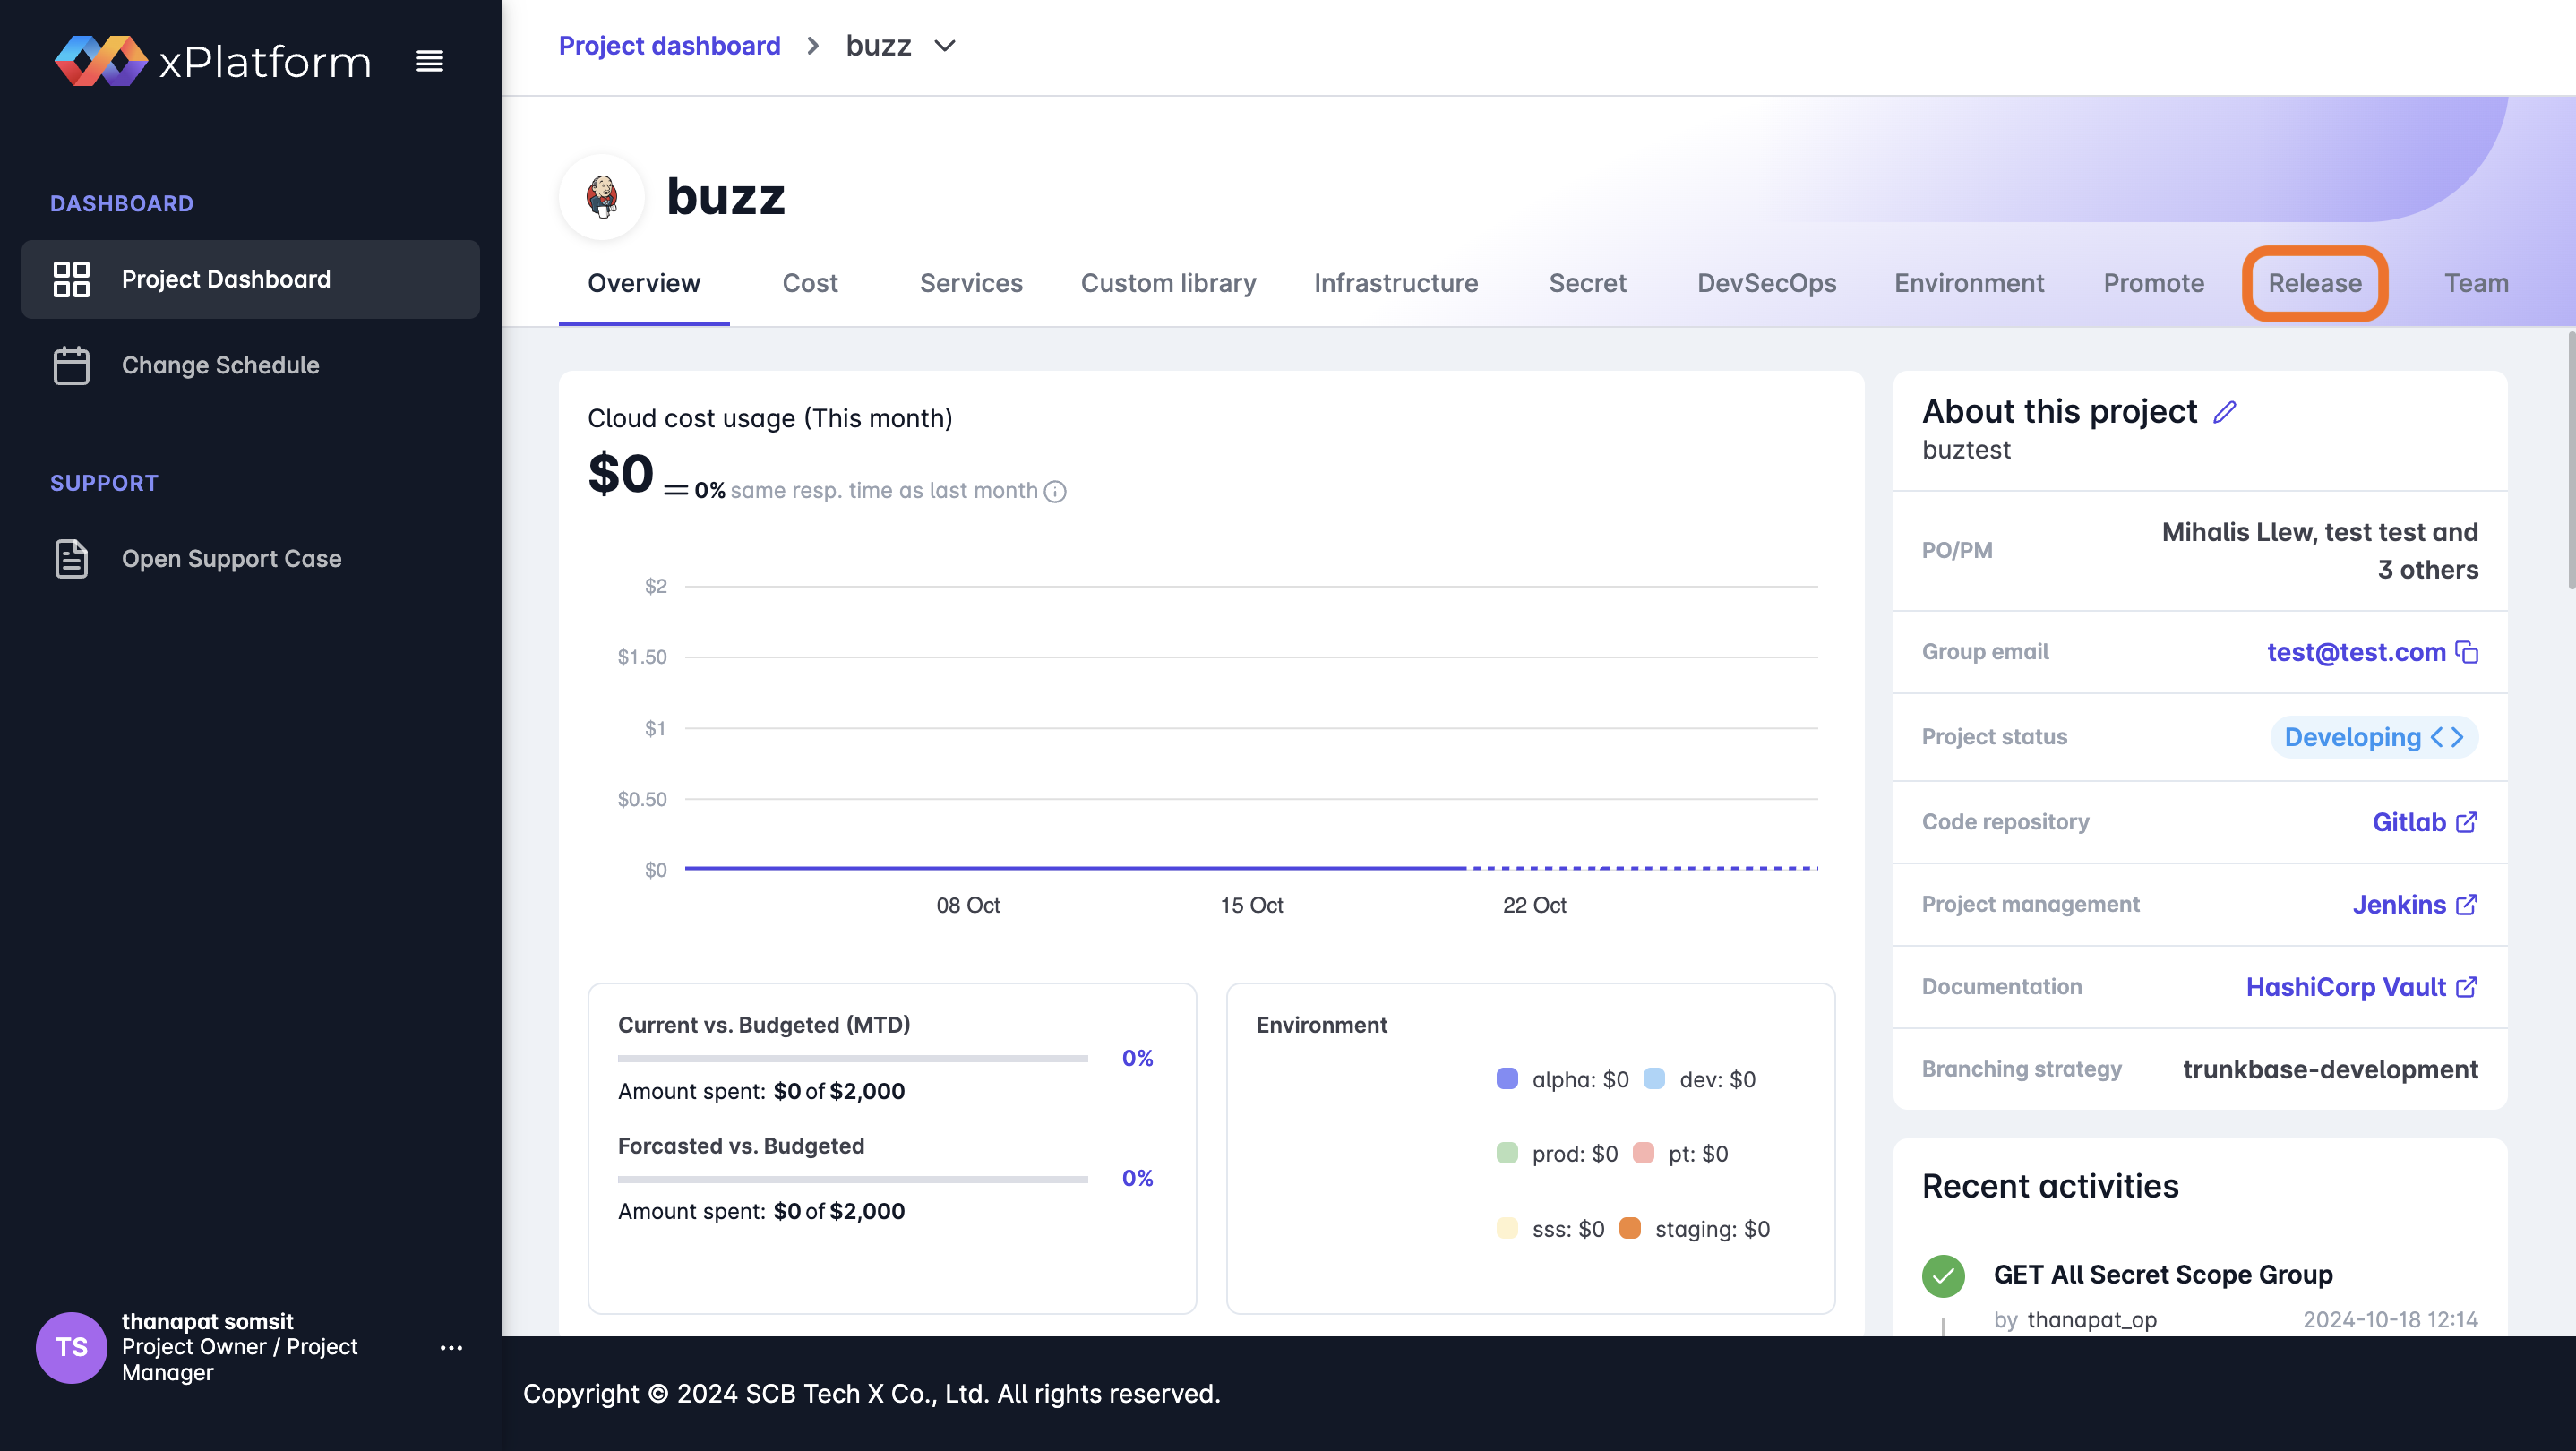
\includegraphics[width=\linewidth]{resources/pages/change-runbook/create-activity/1.png}

    \vspace{1in}

    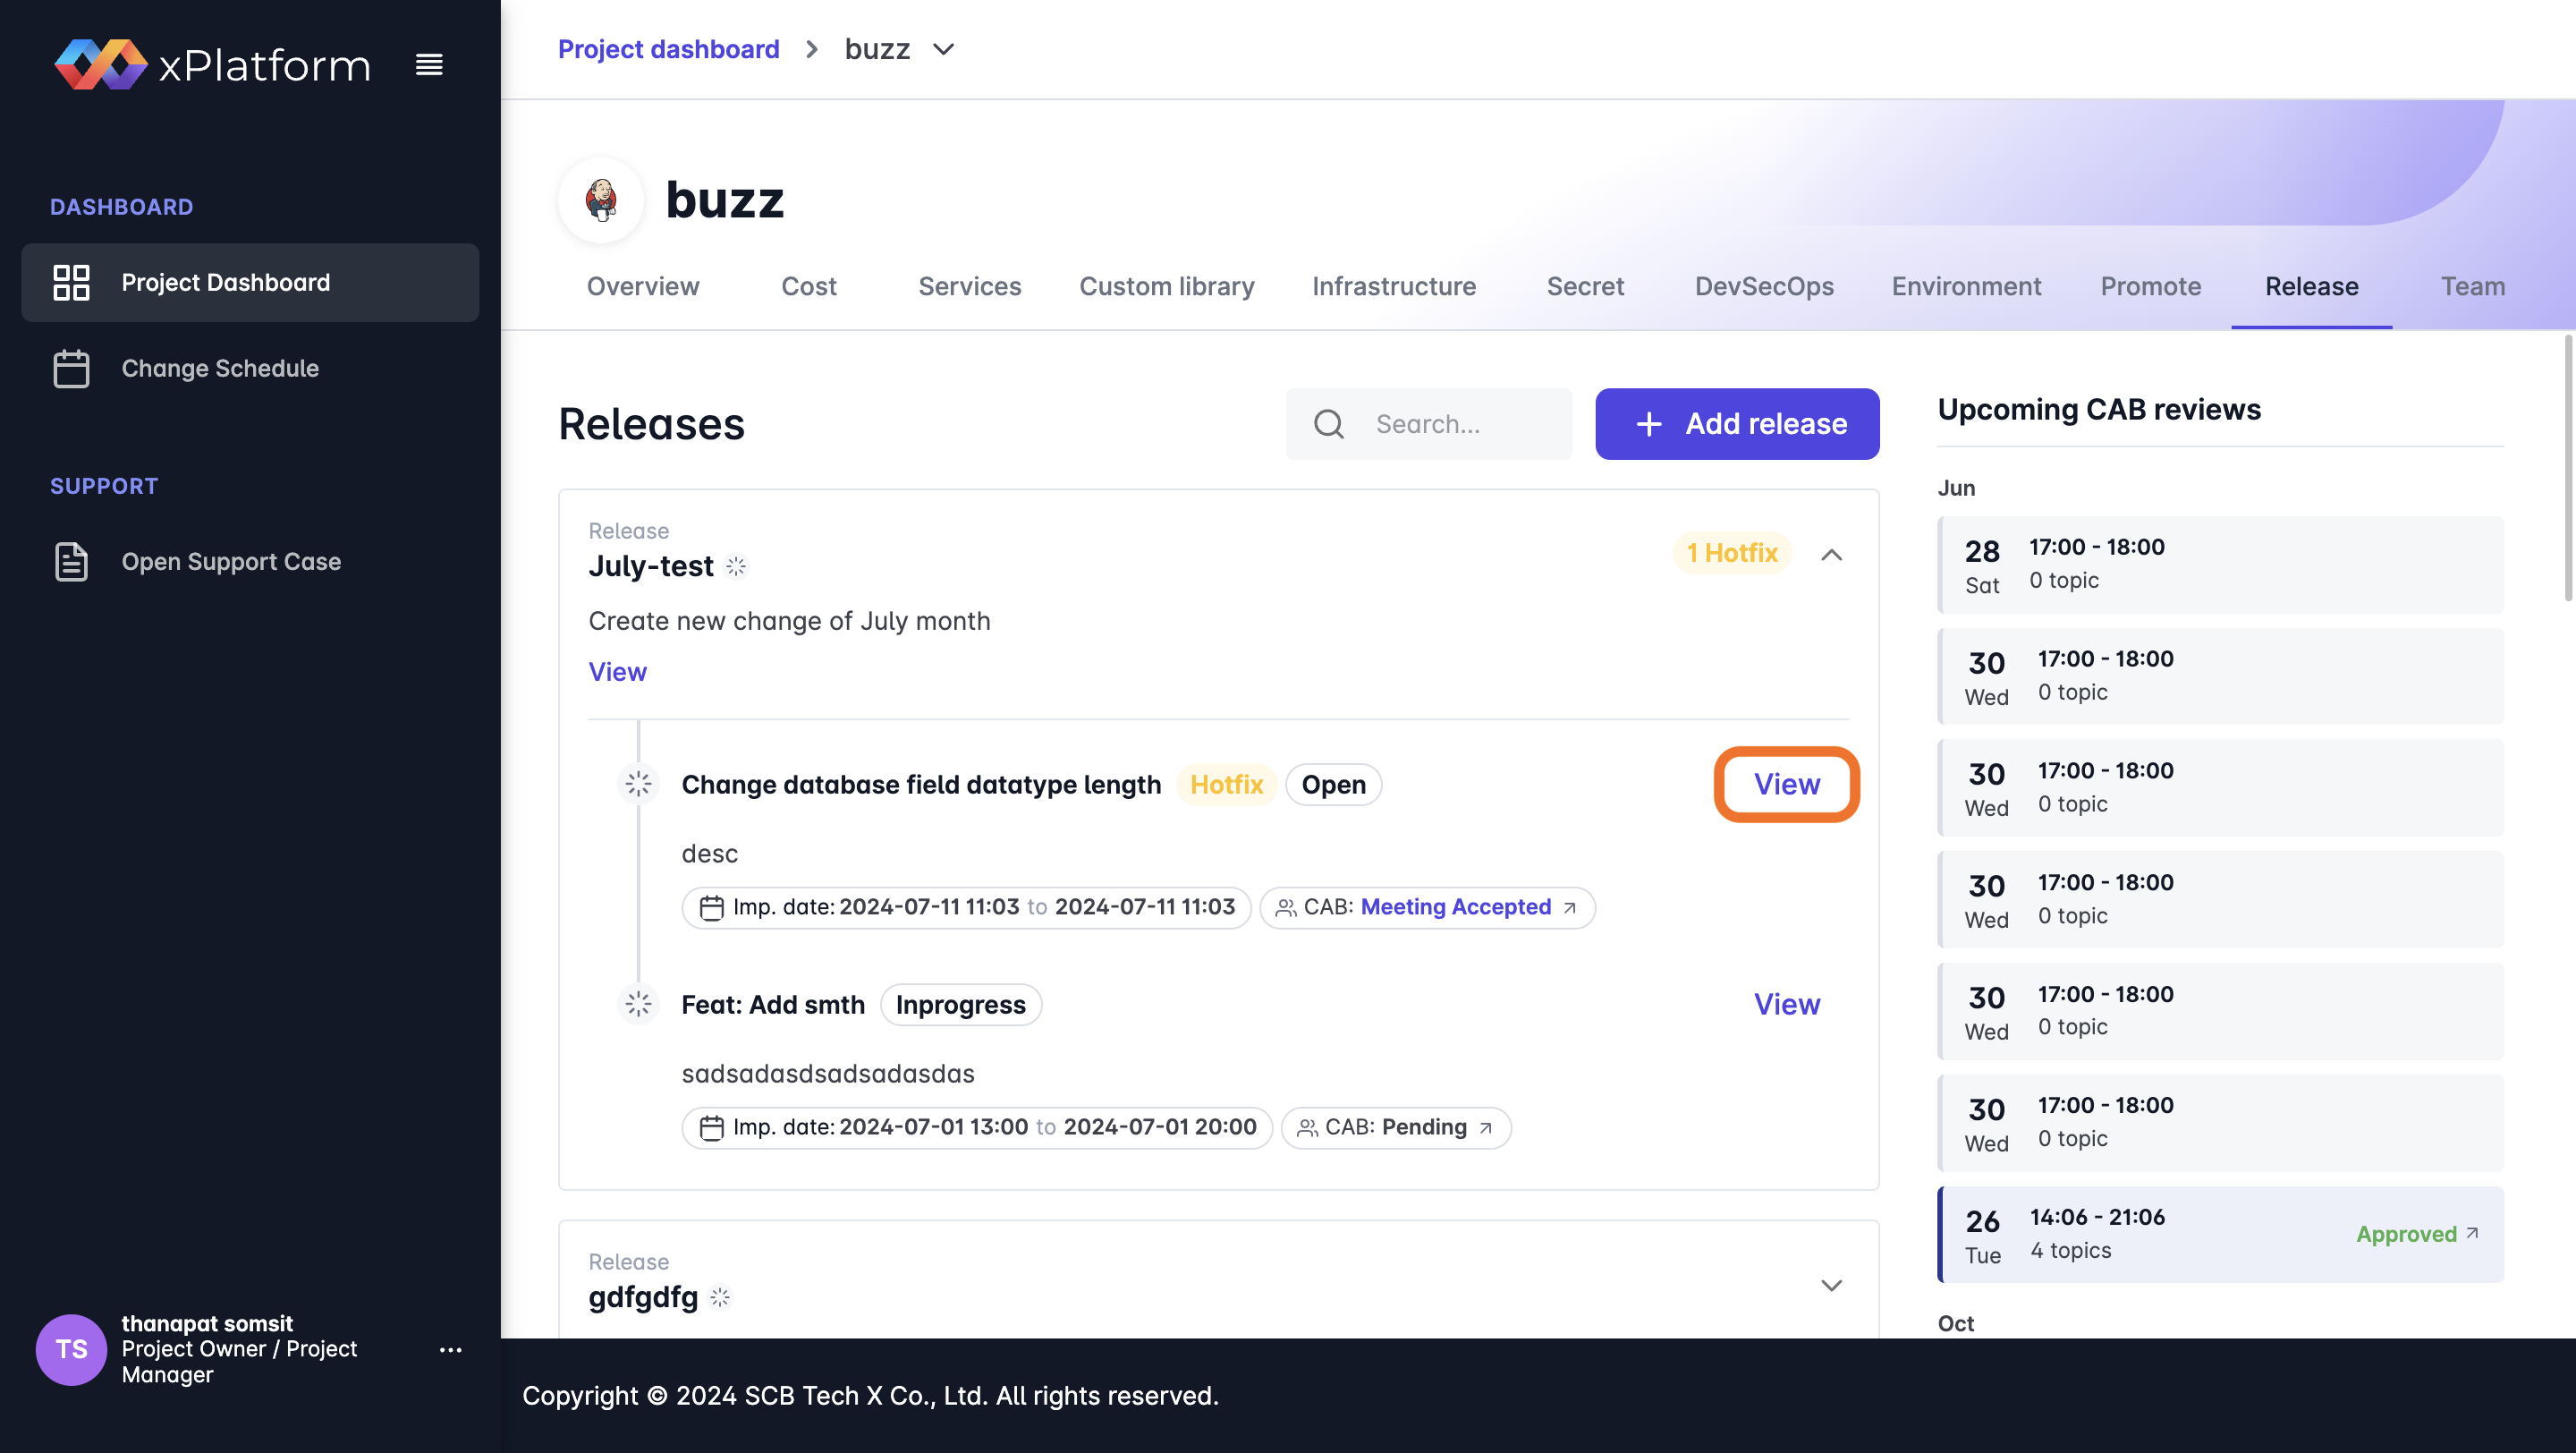
\includegraphics[width=\linewidth]{resources/pages/change-runbook/create-activity/2.png}
\end{center}
\begin{center}
    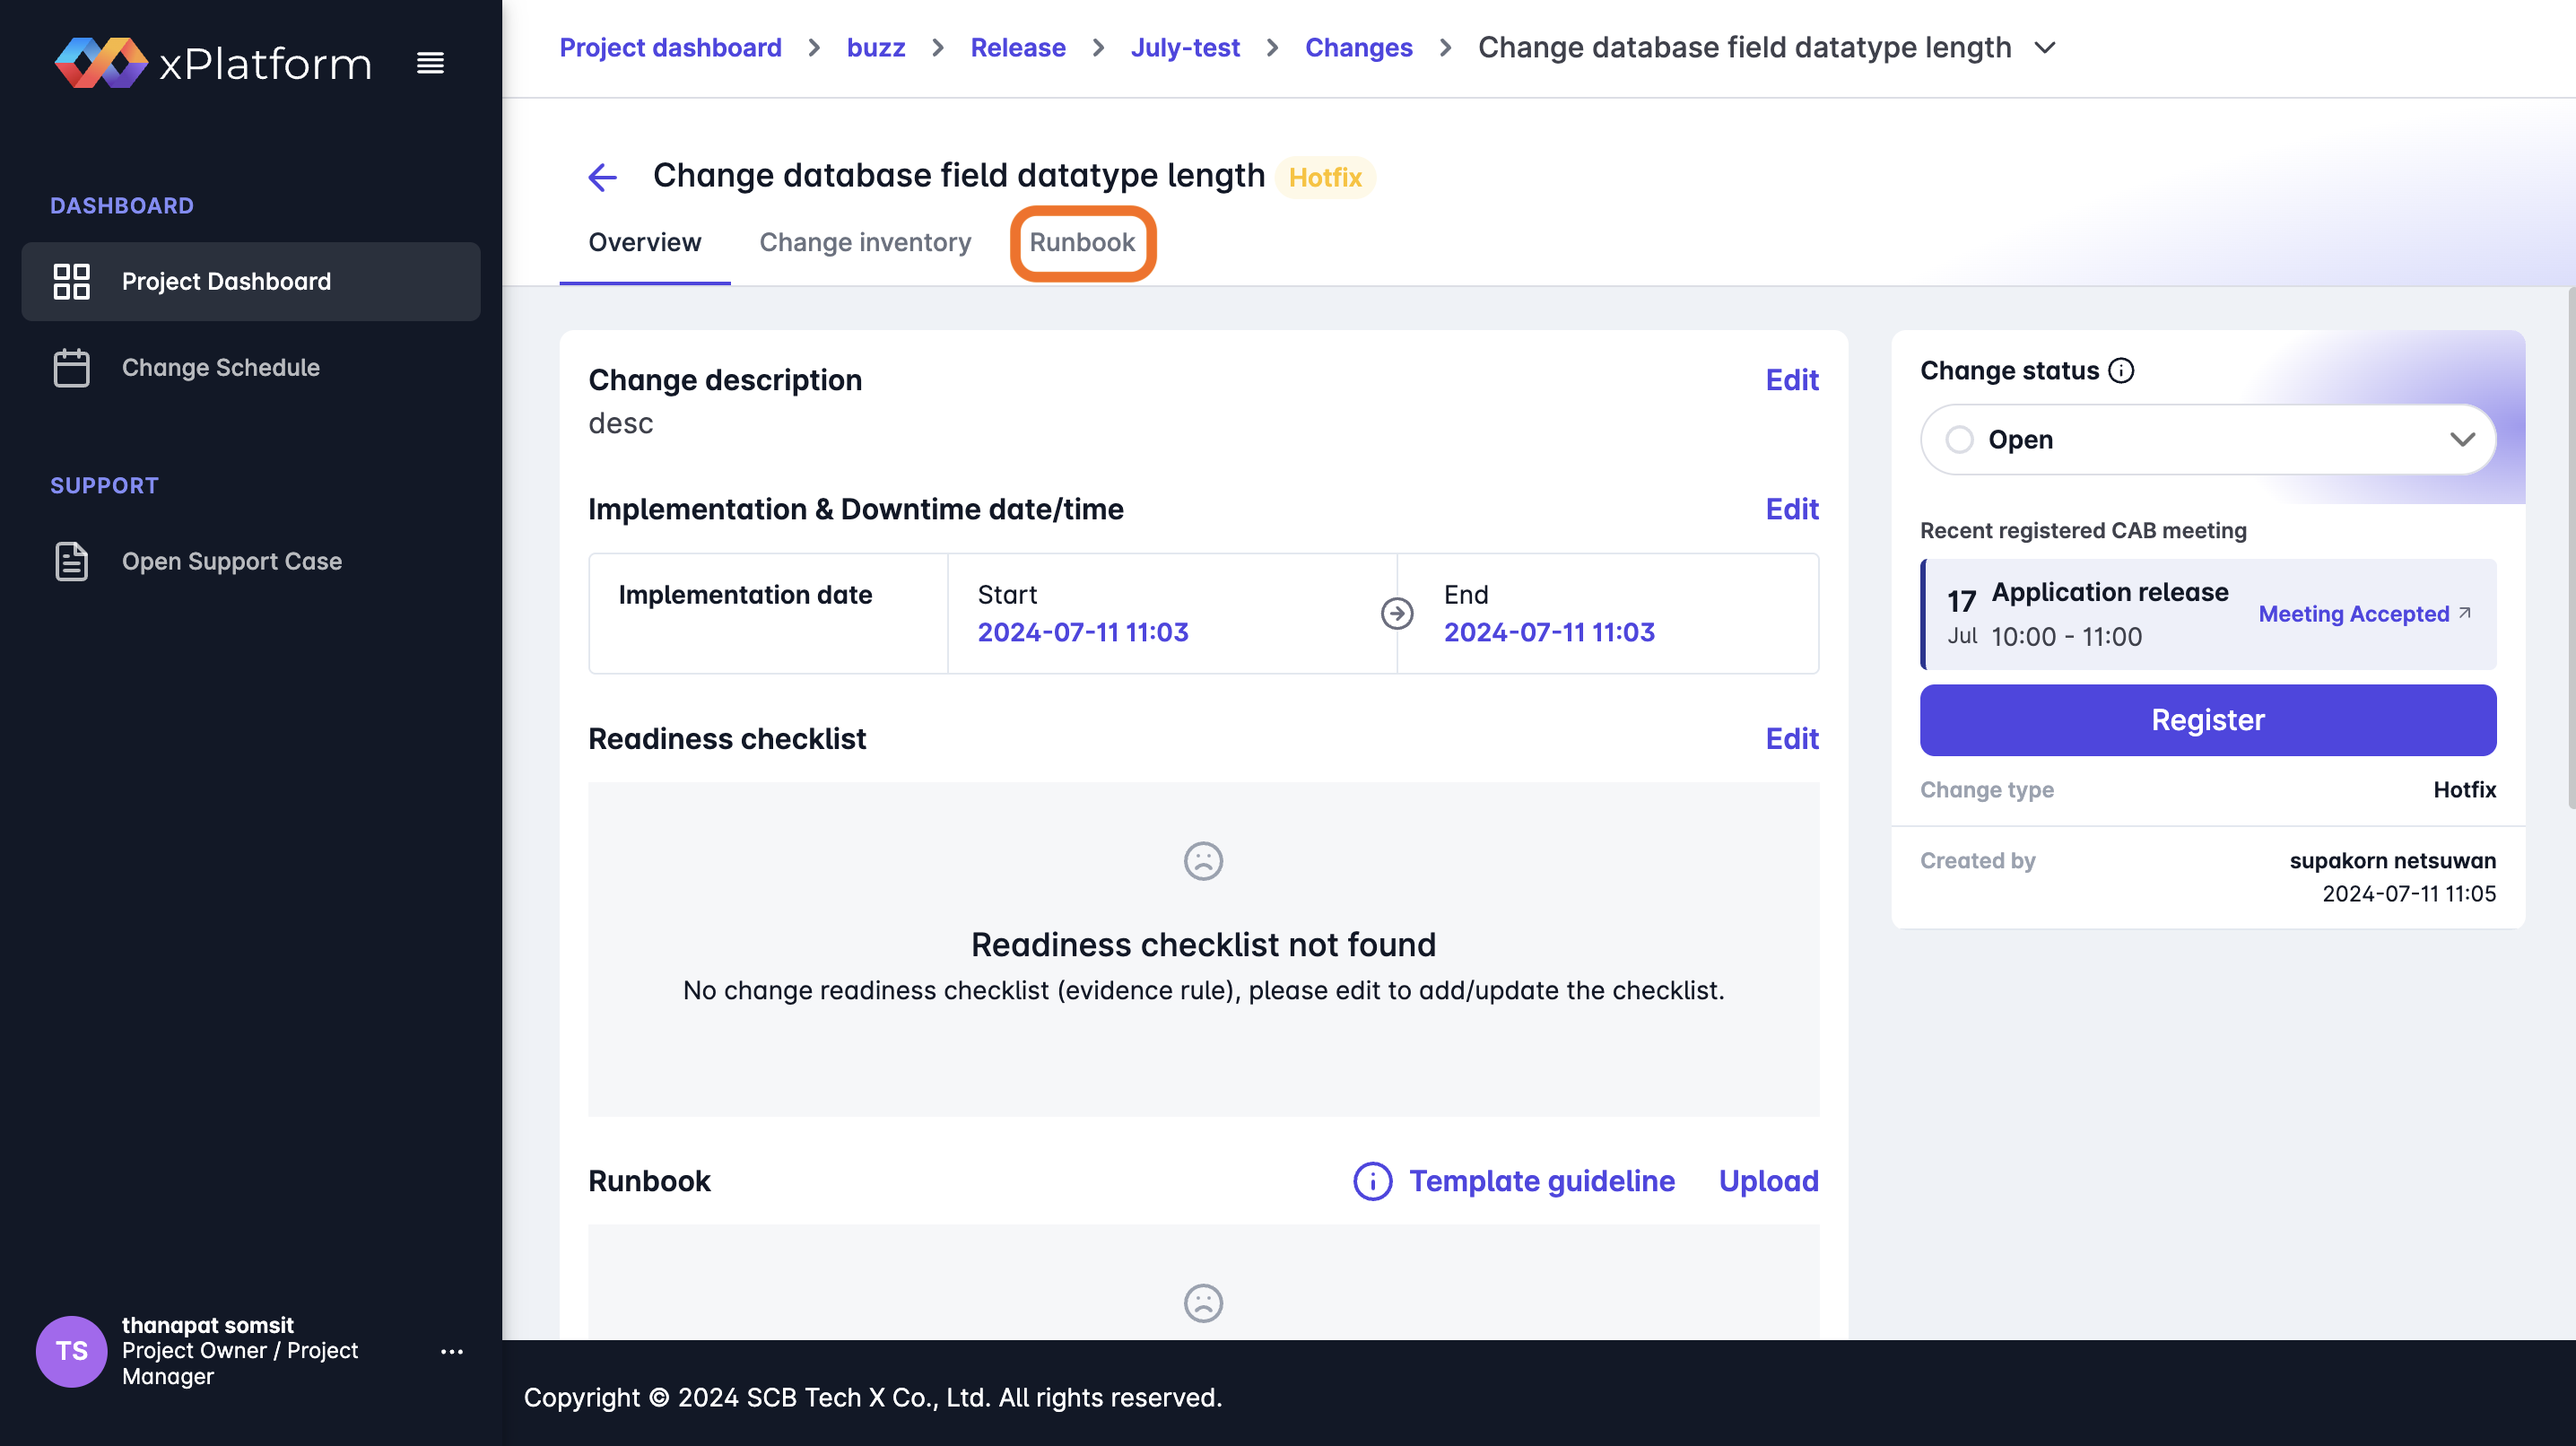
\includegraphics[width=\linewidth]{resources/pages/change-runbook/create-activity/3.png}

    \vspace{1in}

    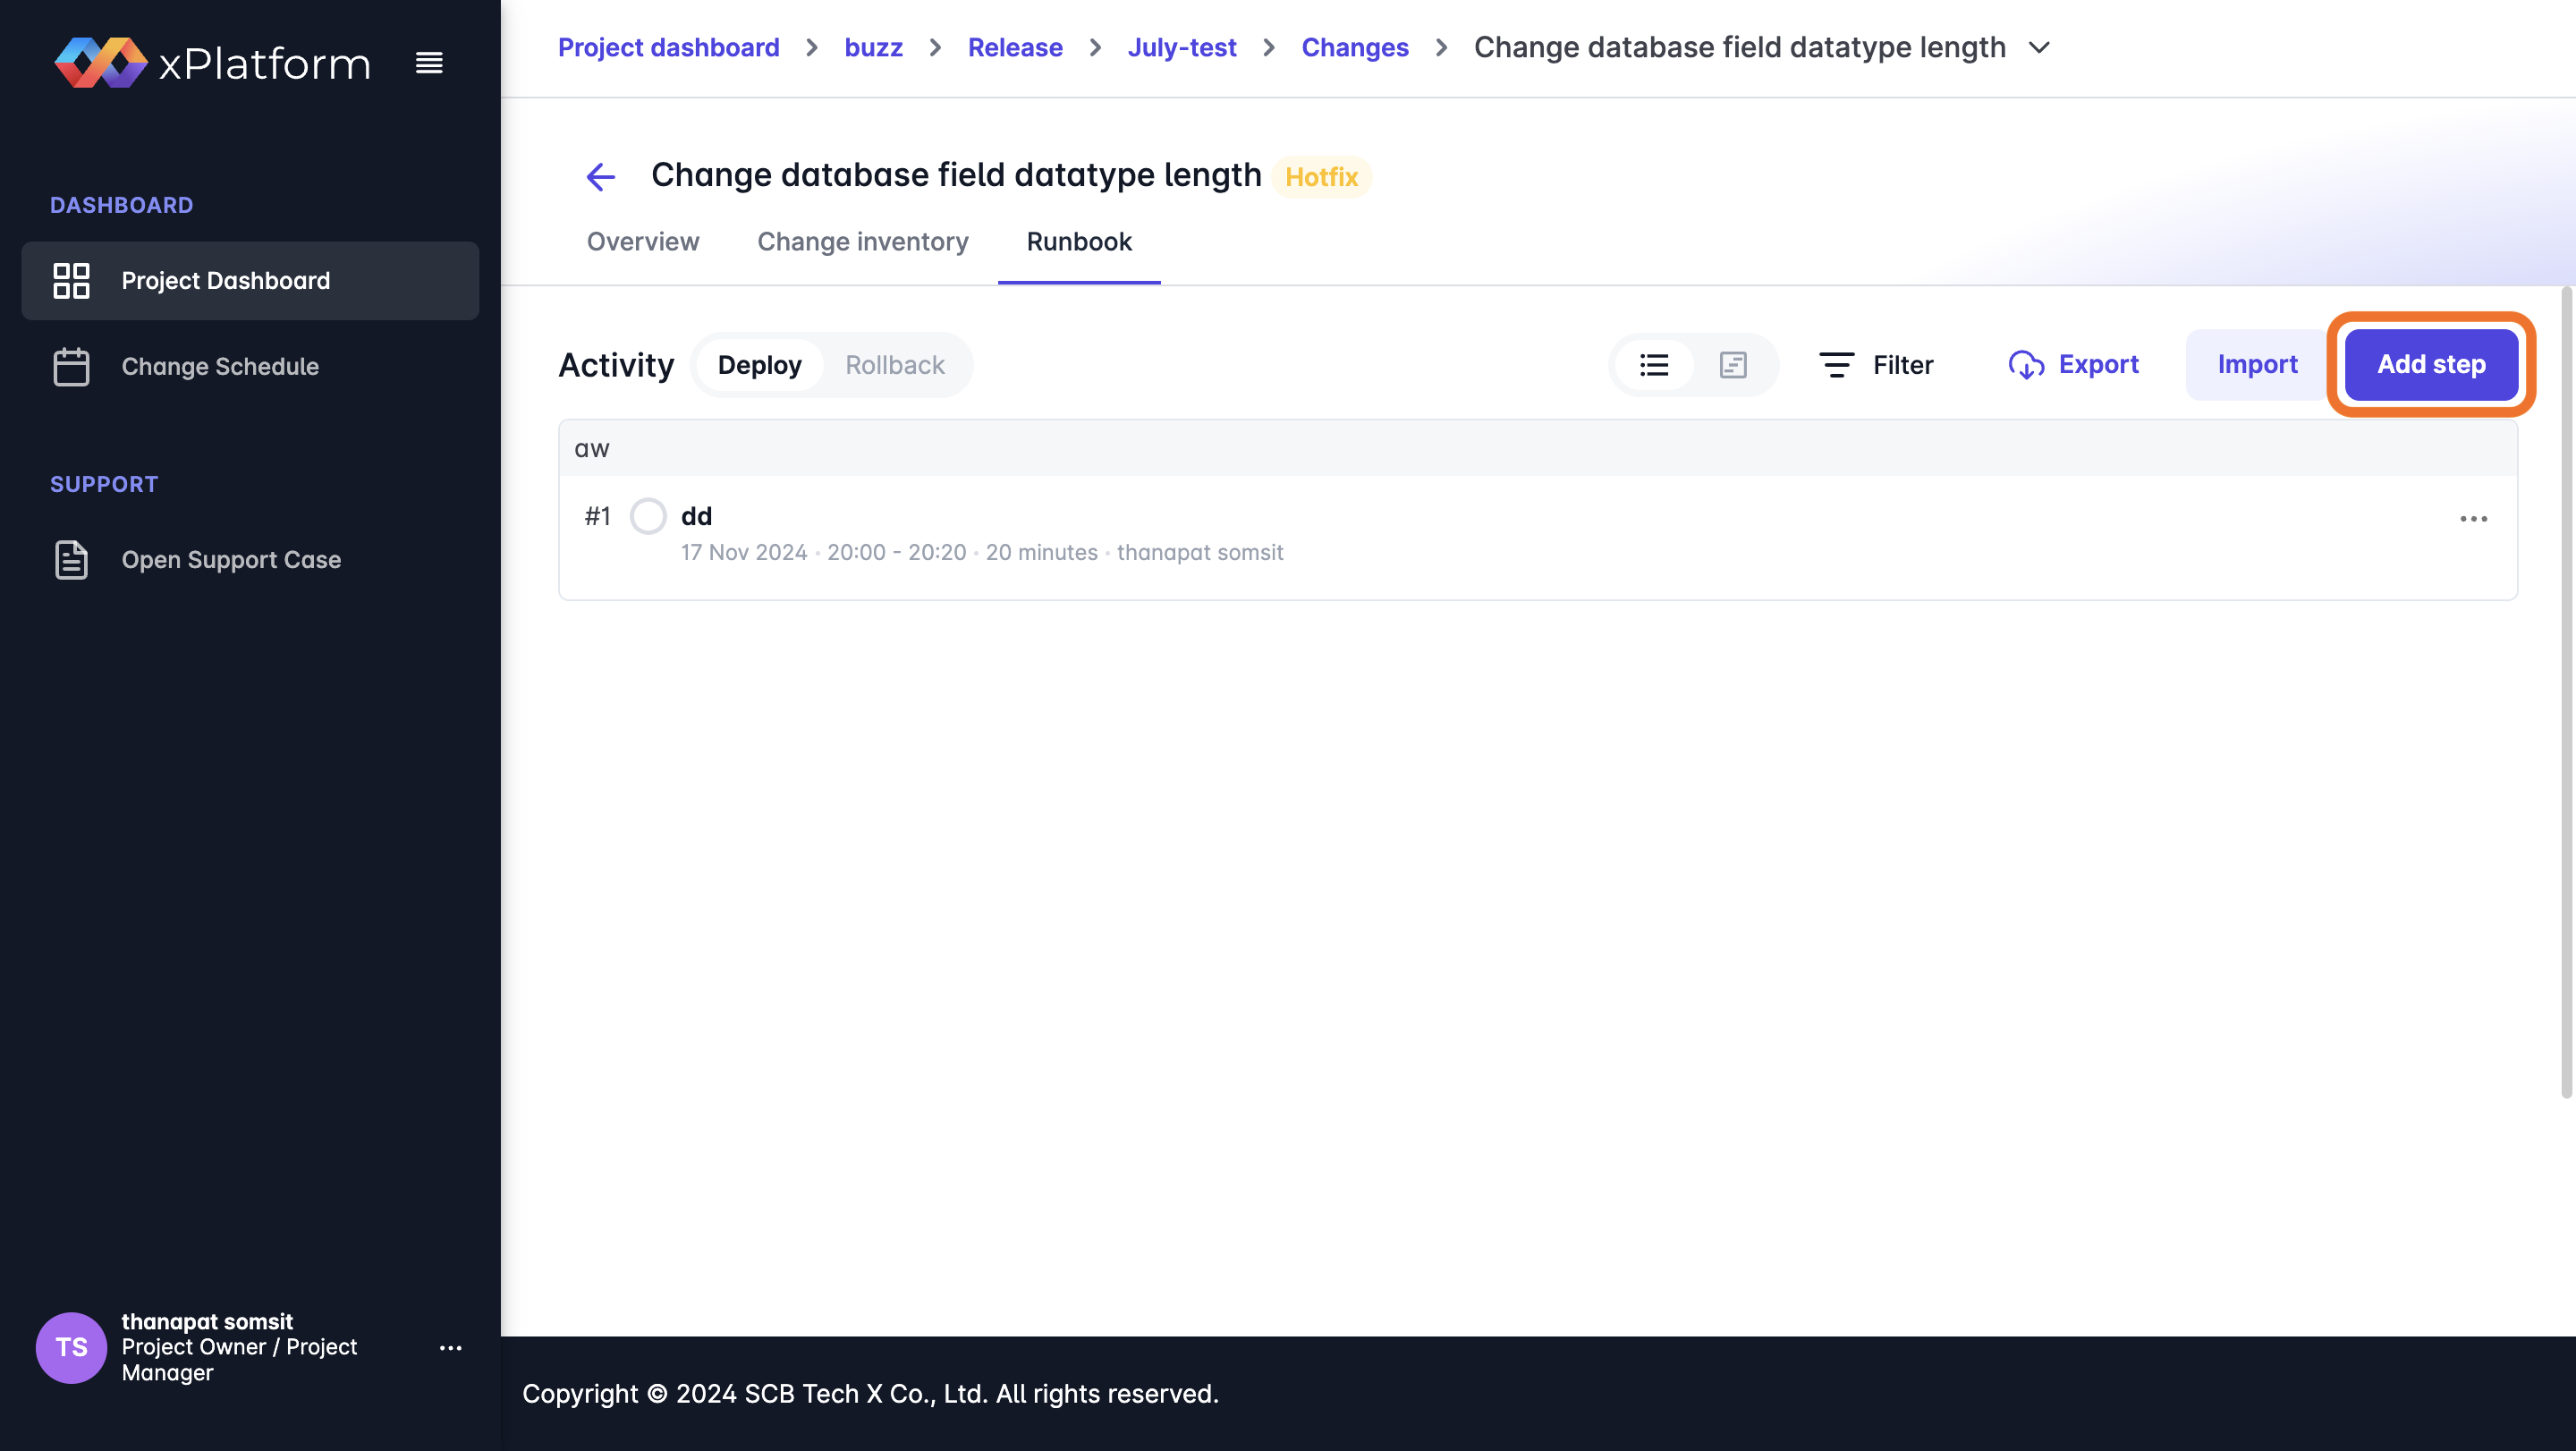
\includegraphics[width=\linewidth]{resources/pages/change-runbook/create-activity/4.png}
\end{center}

\begin{figure}[H]
    \begin{center}
        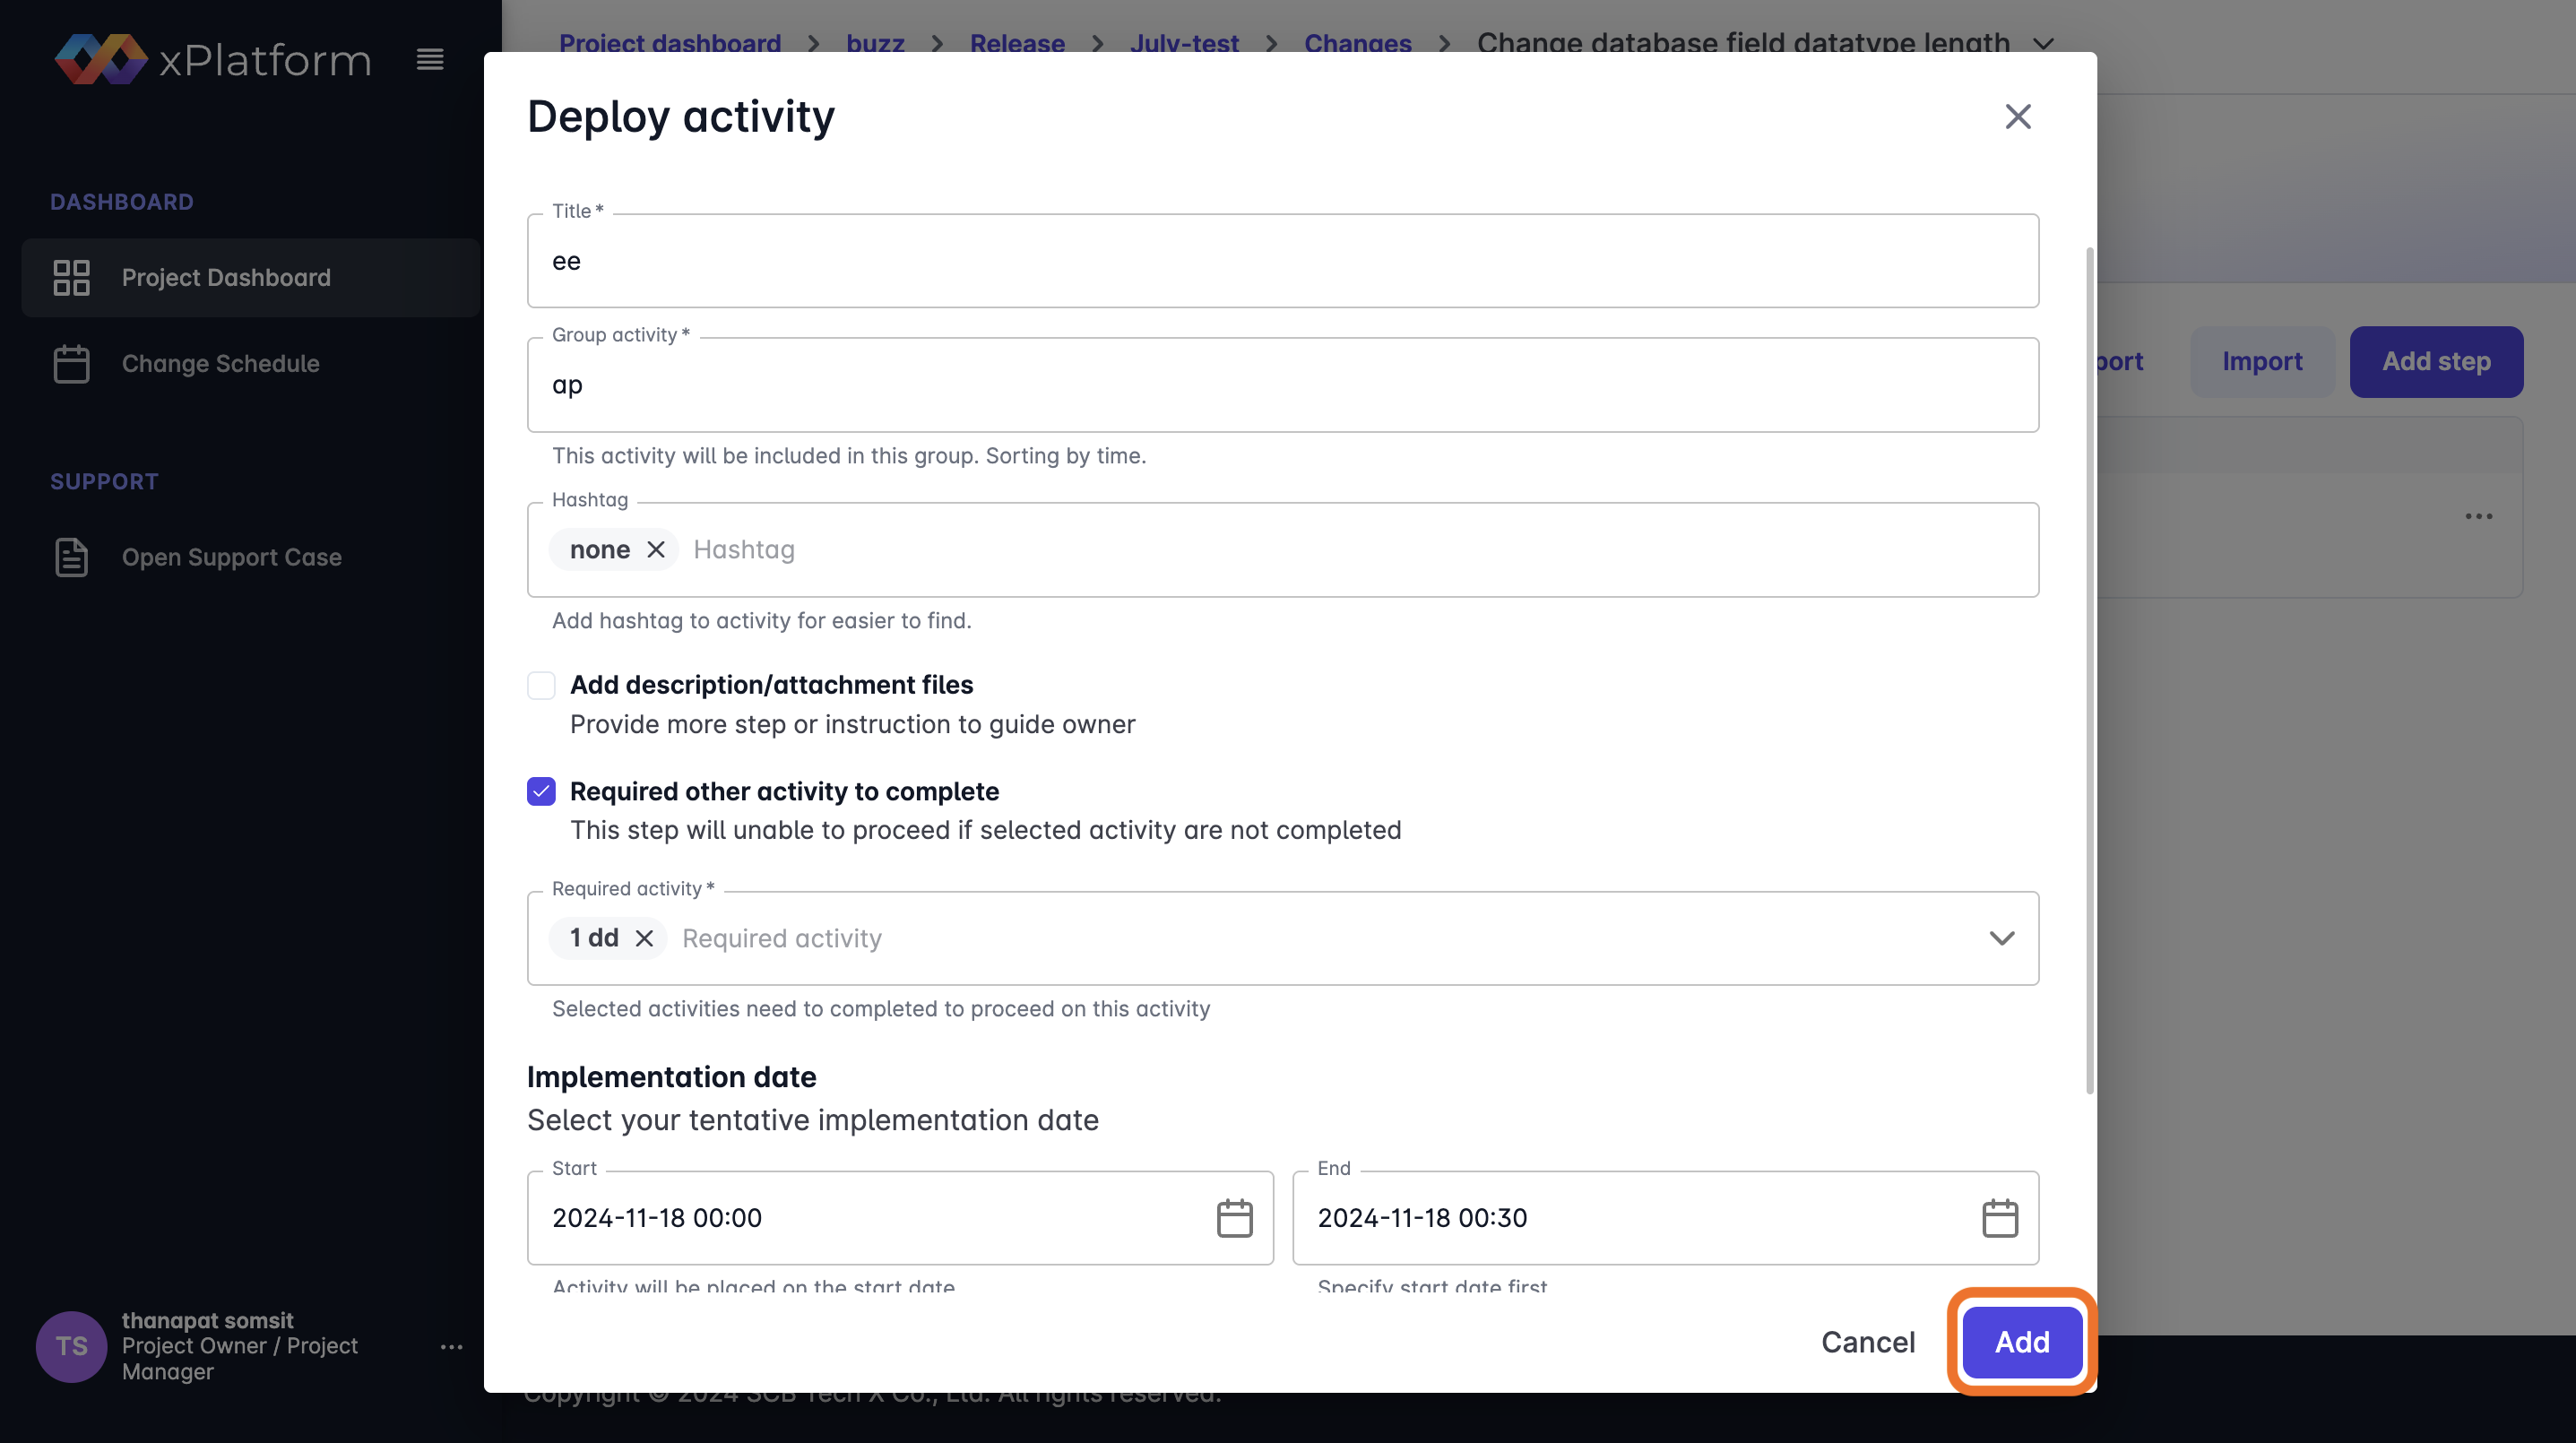
\includegraphics[width=\linewidth]{resources/pages/change-runbook/create-activity/5.png}
    
        \vspace{1in}
    
        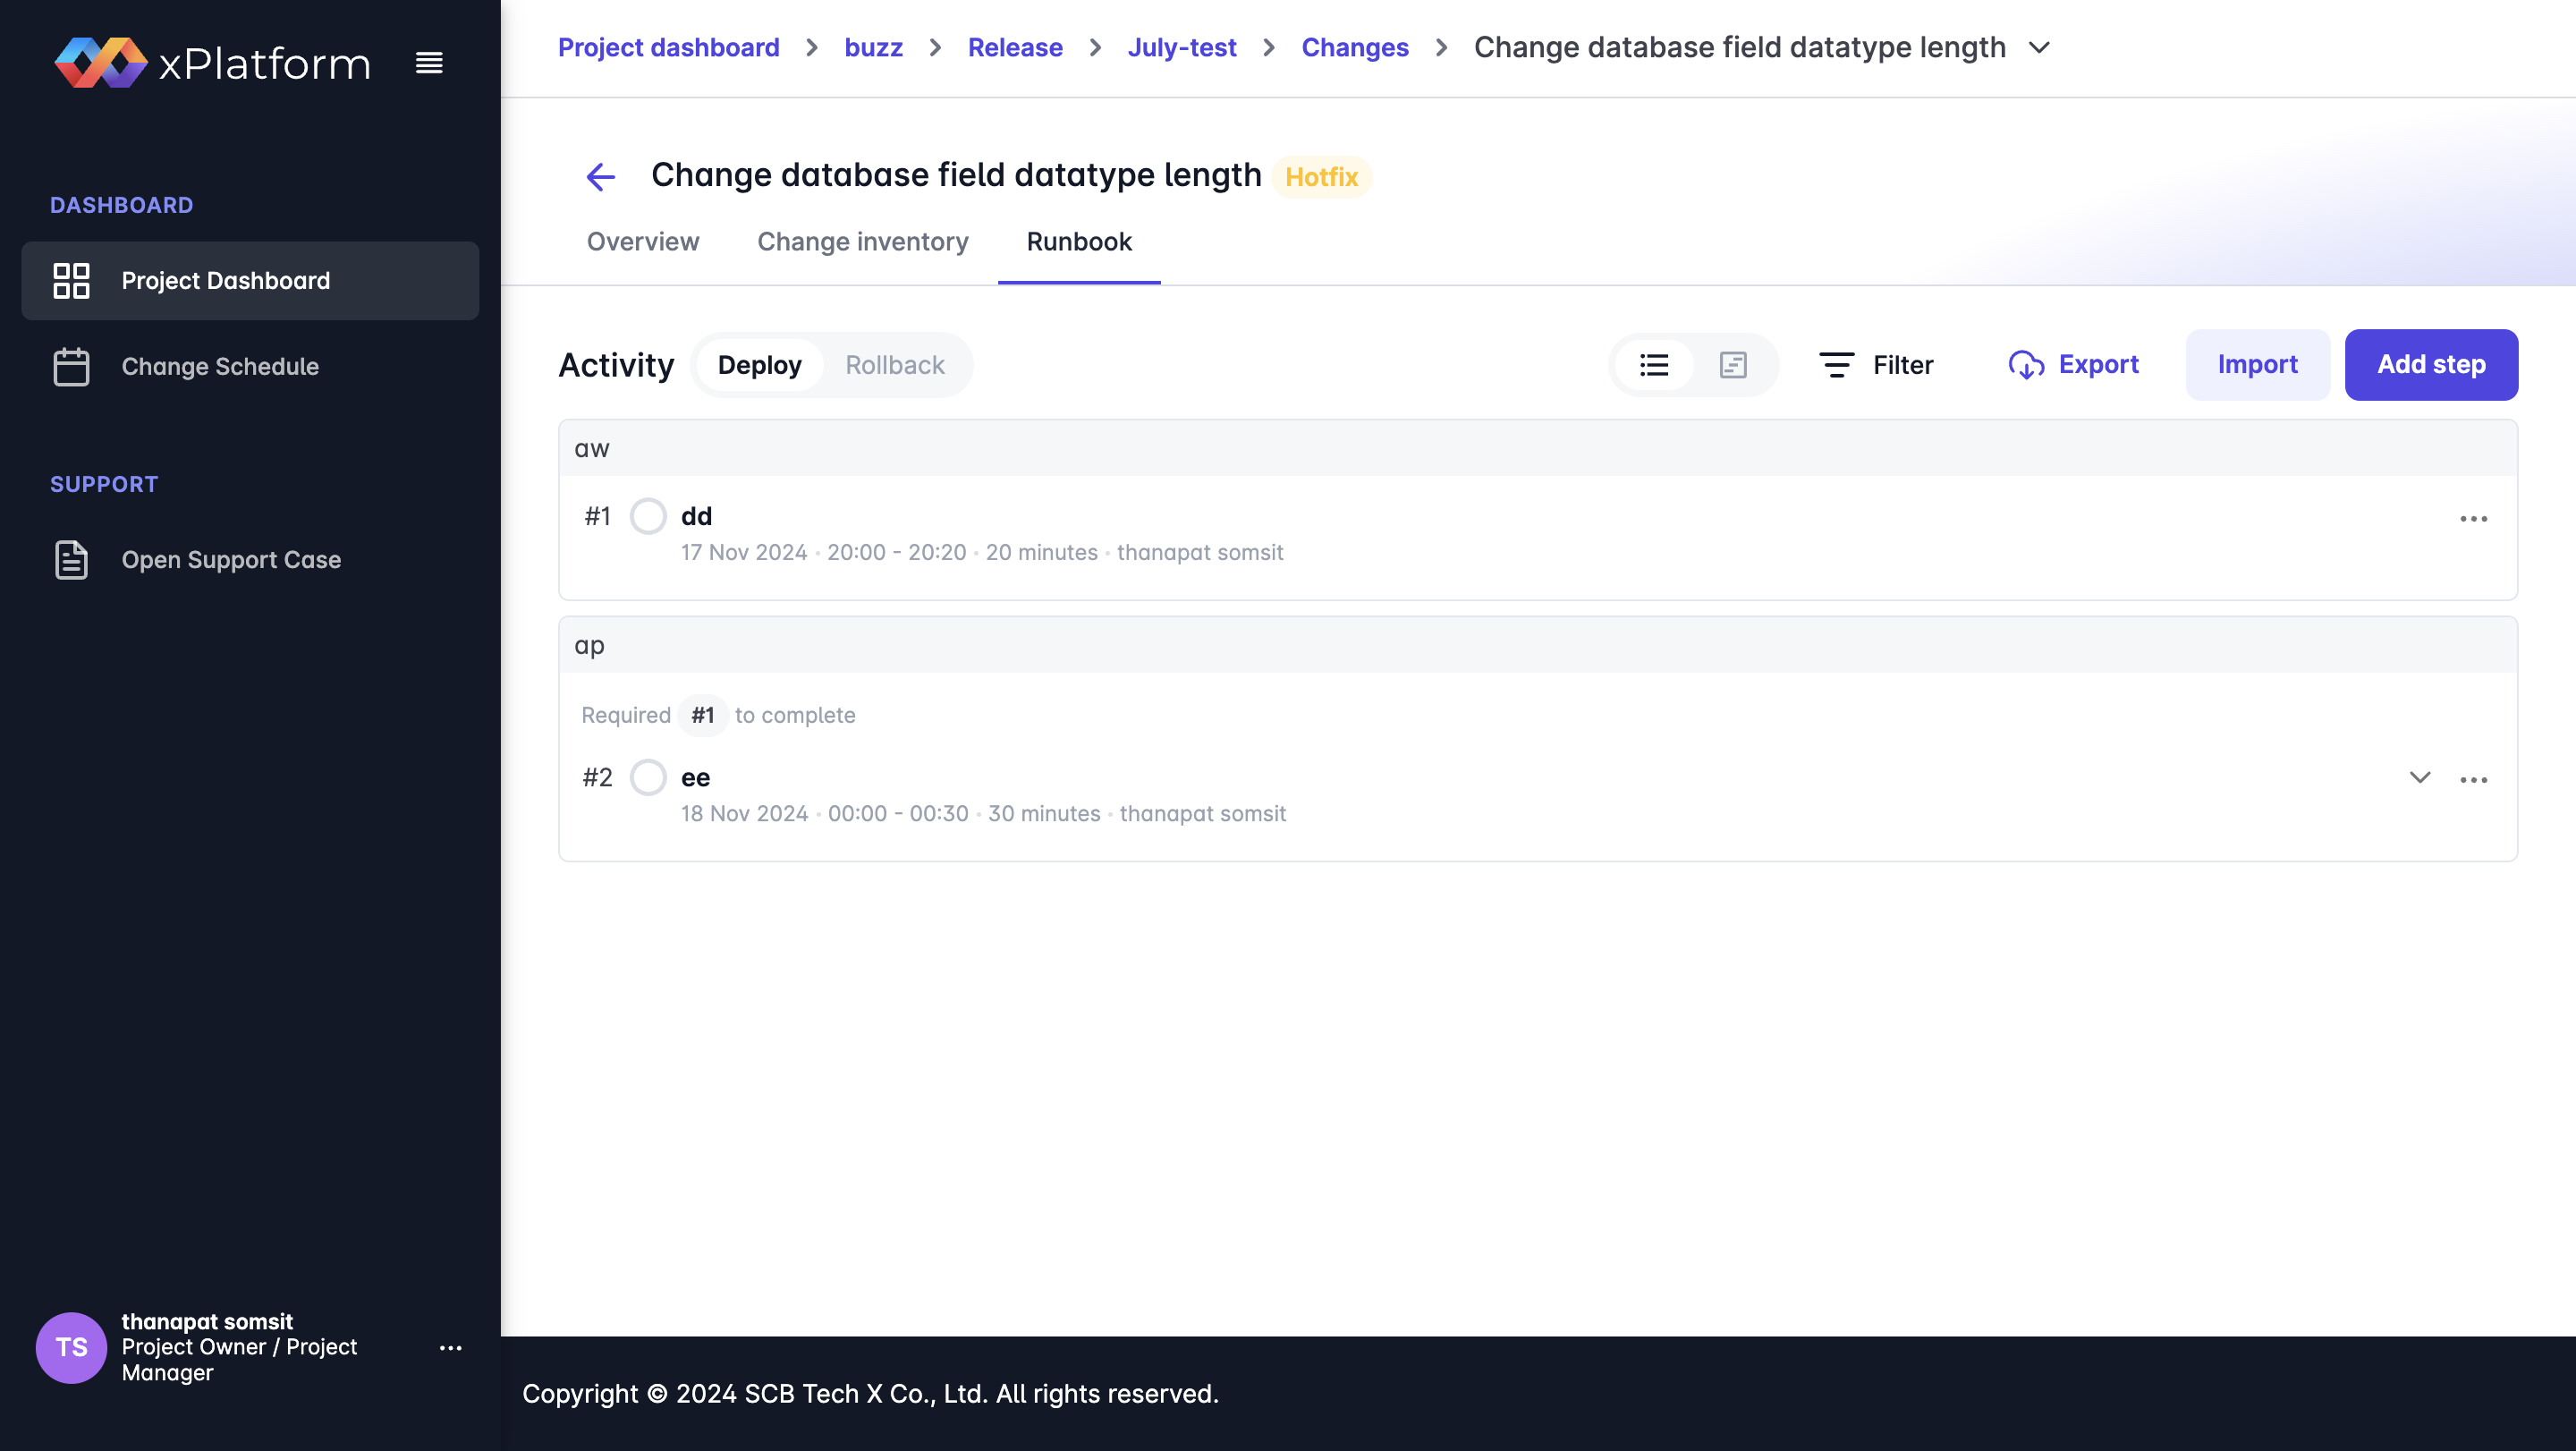
\includegraphics[width=\linewidth]{resources/pages/change-runbook/create-activity/6.png}
    \end{center}
    \caption[การสร้าง Activity]{การสร้าง Activity}
  \label{fig:create-activity}
\end{figure}

\newpage
\subsection{การเปลี่ยนแปลง Activity}
\begin{center}
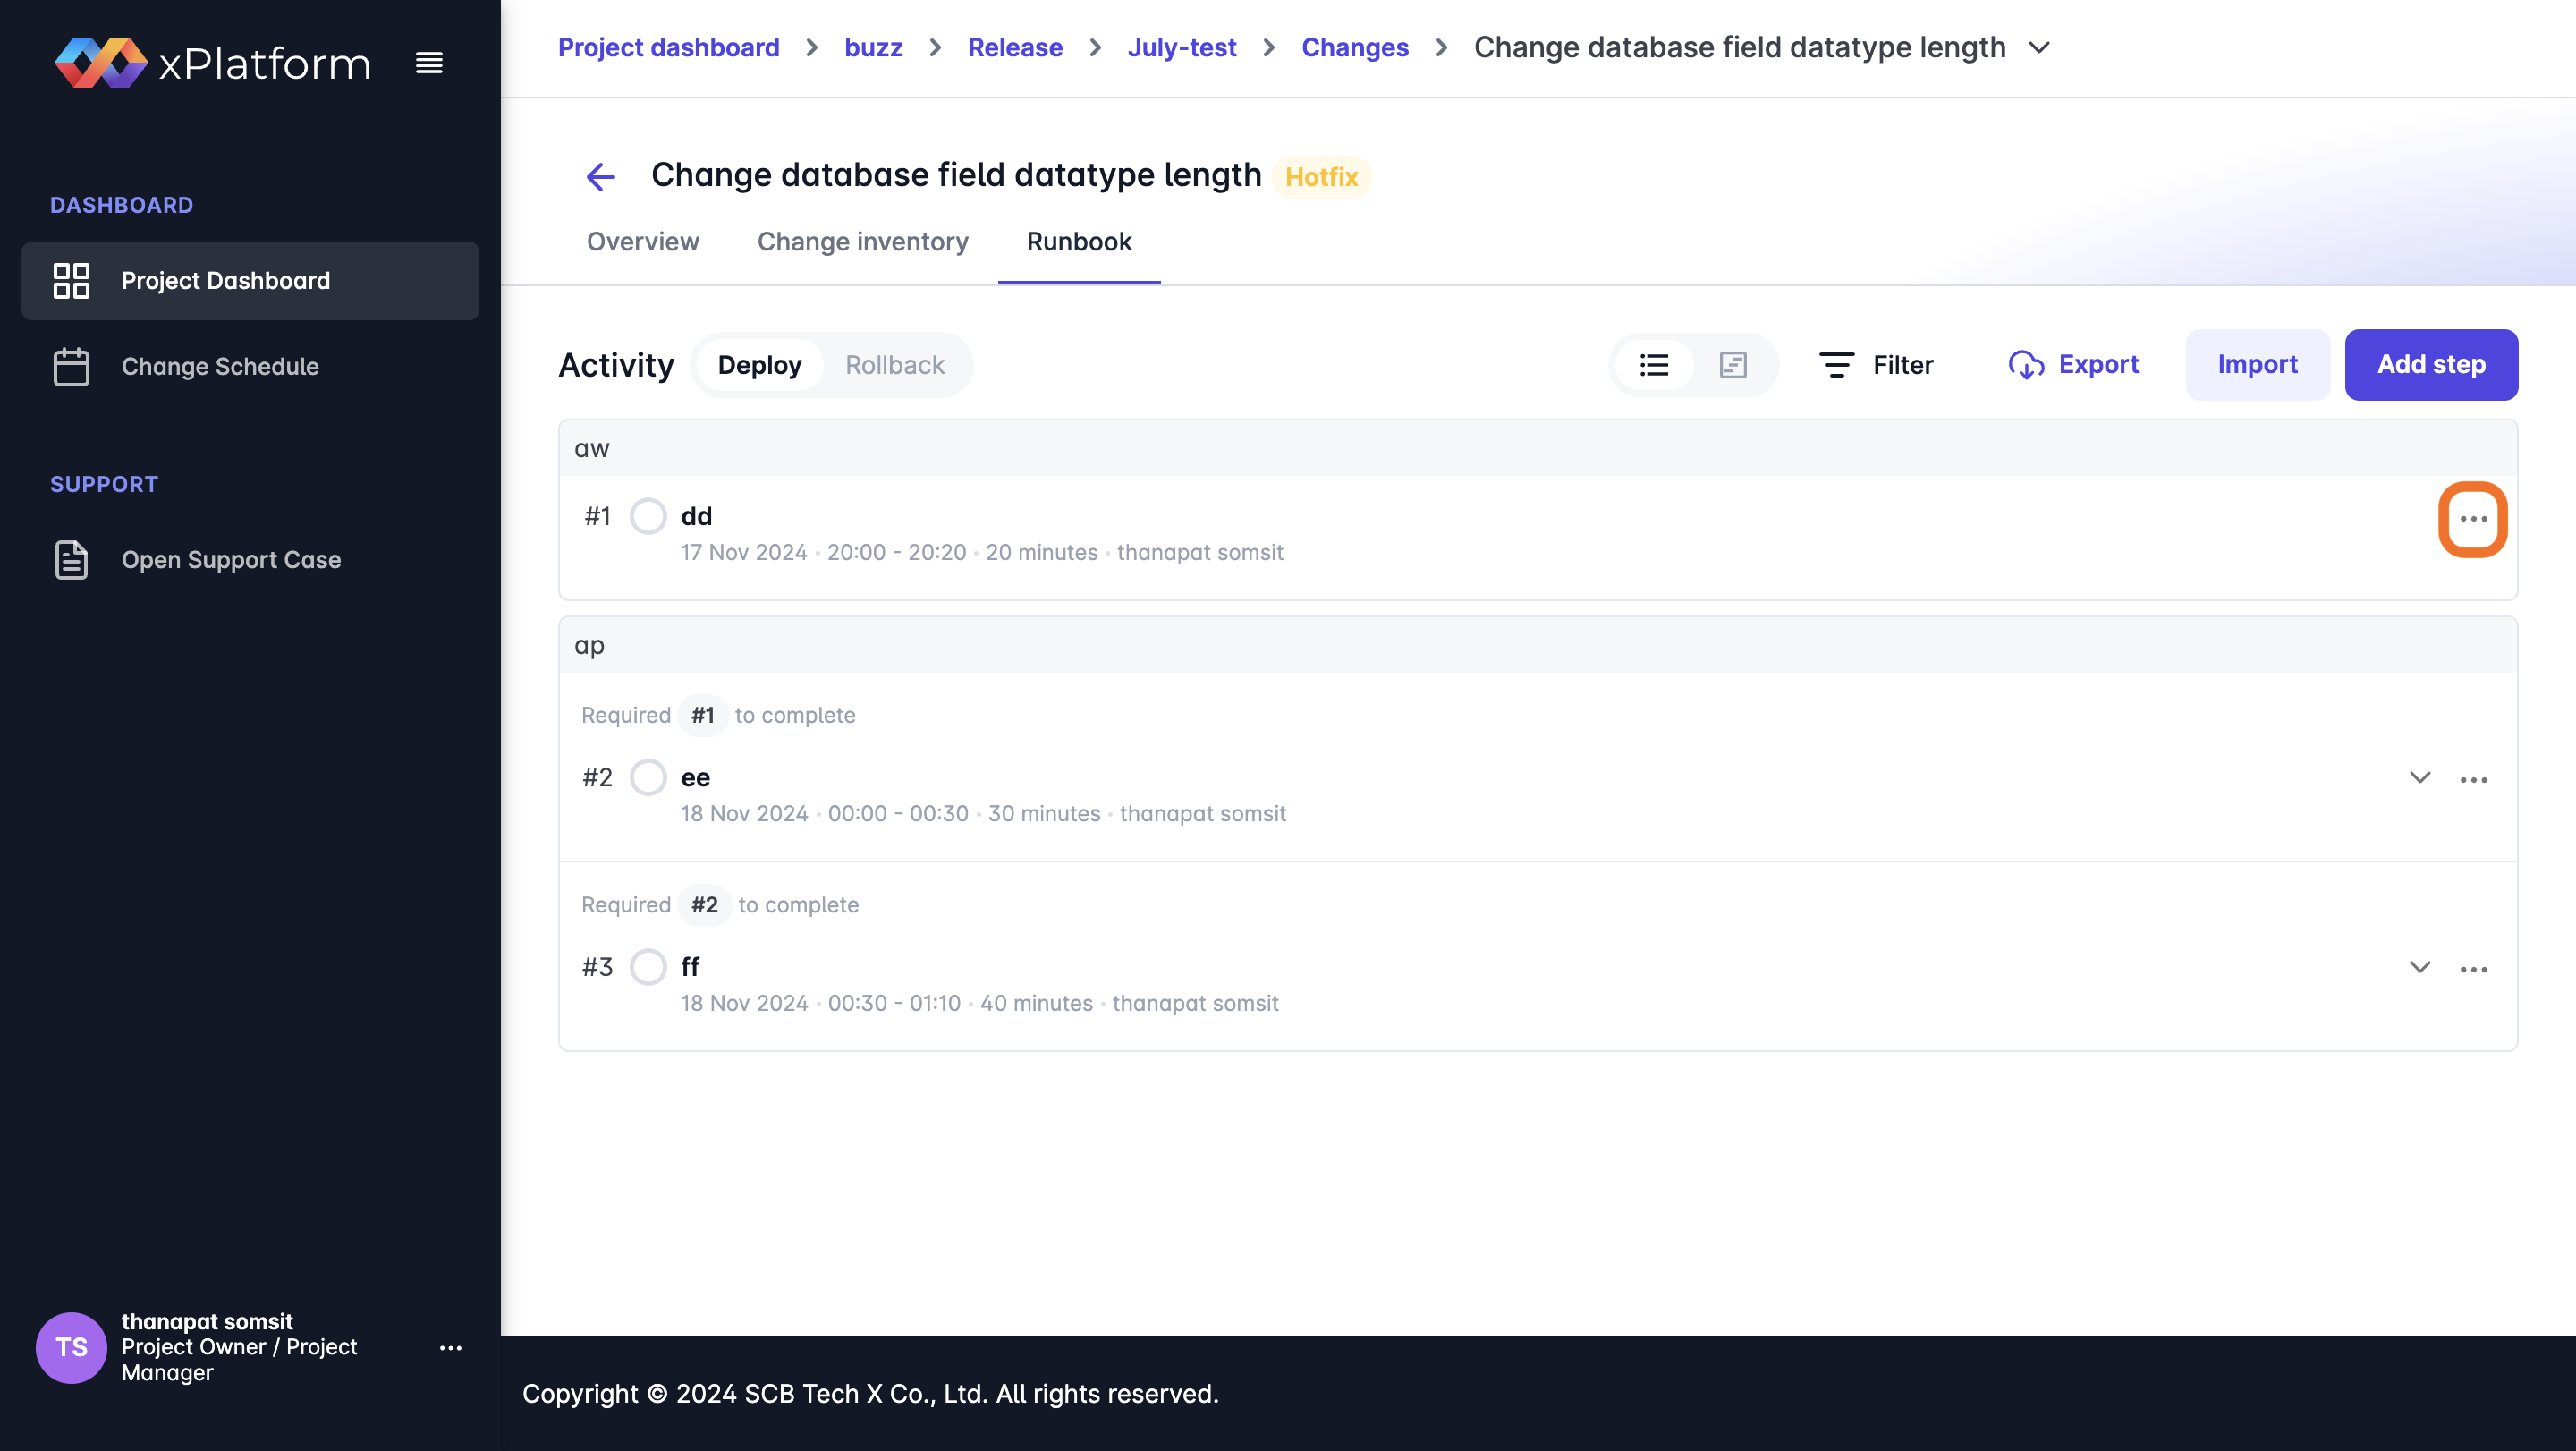
\includegraphics[width=\linewidth]{resources/pages/change-runbook/update-activity/7.png}

\vspace{1in}

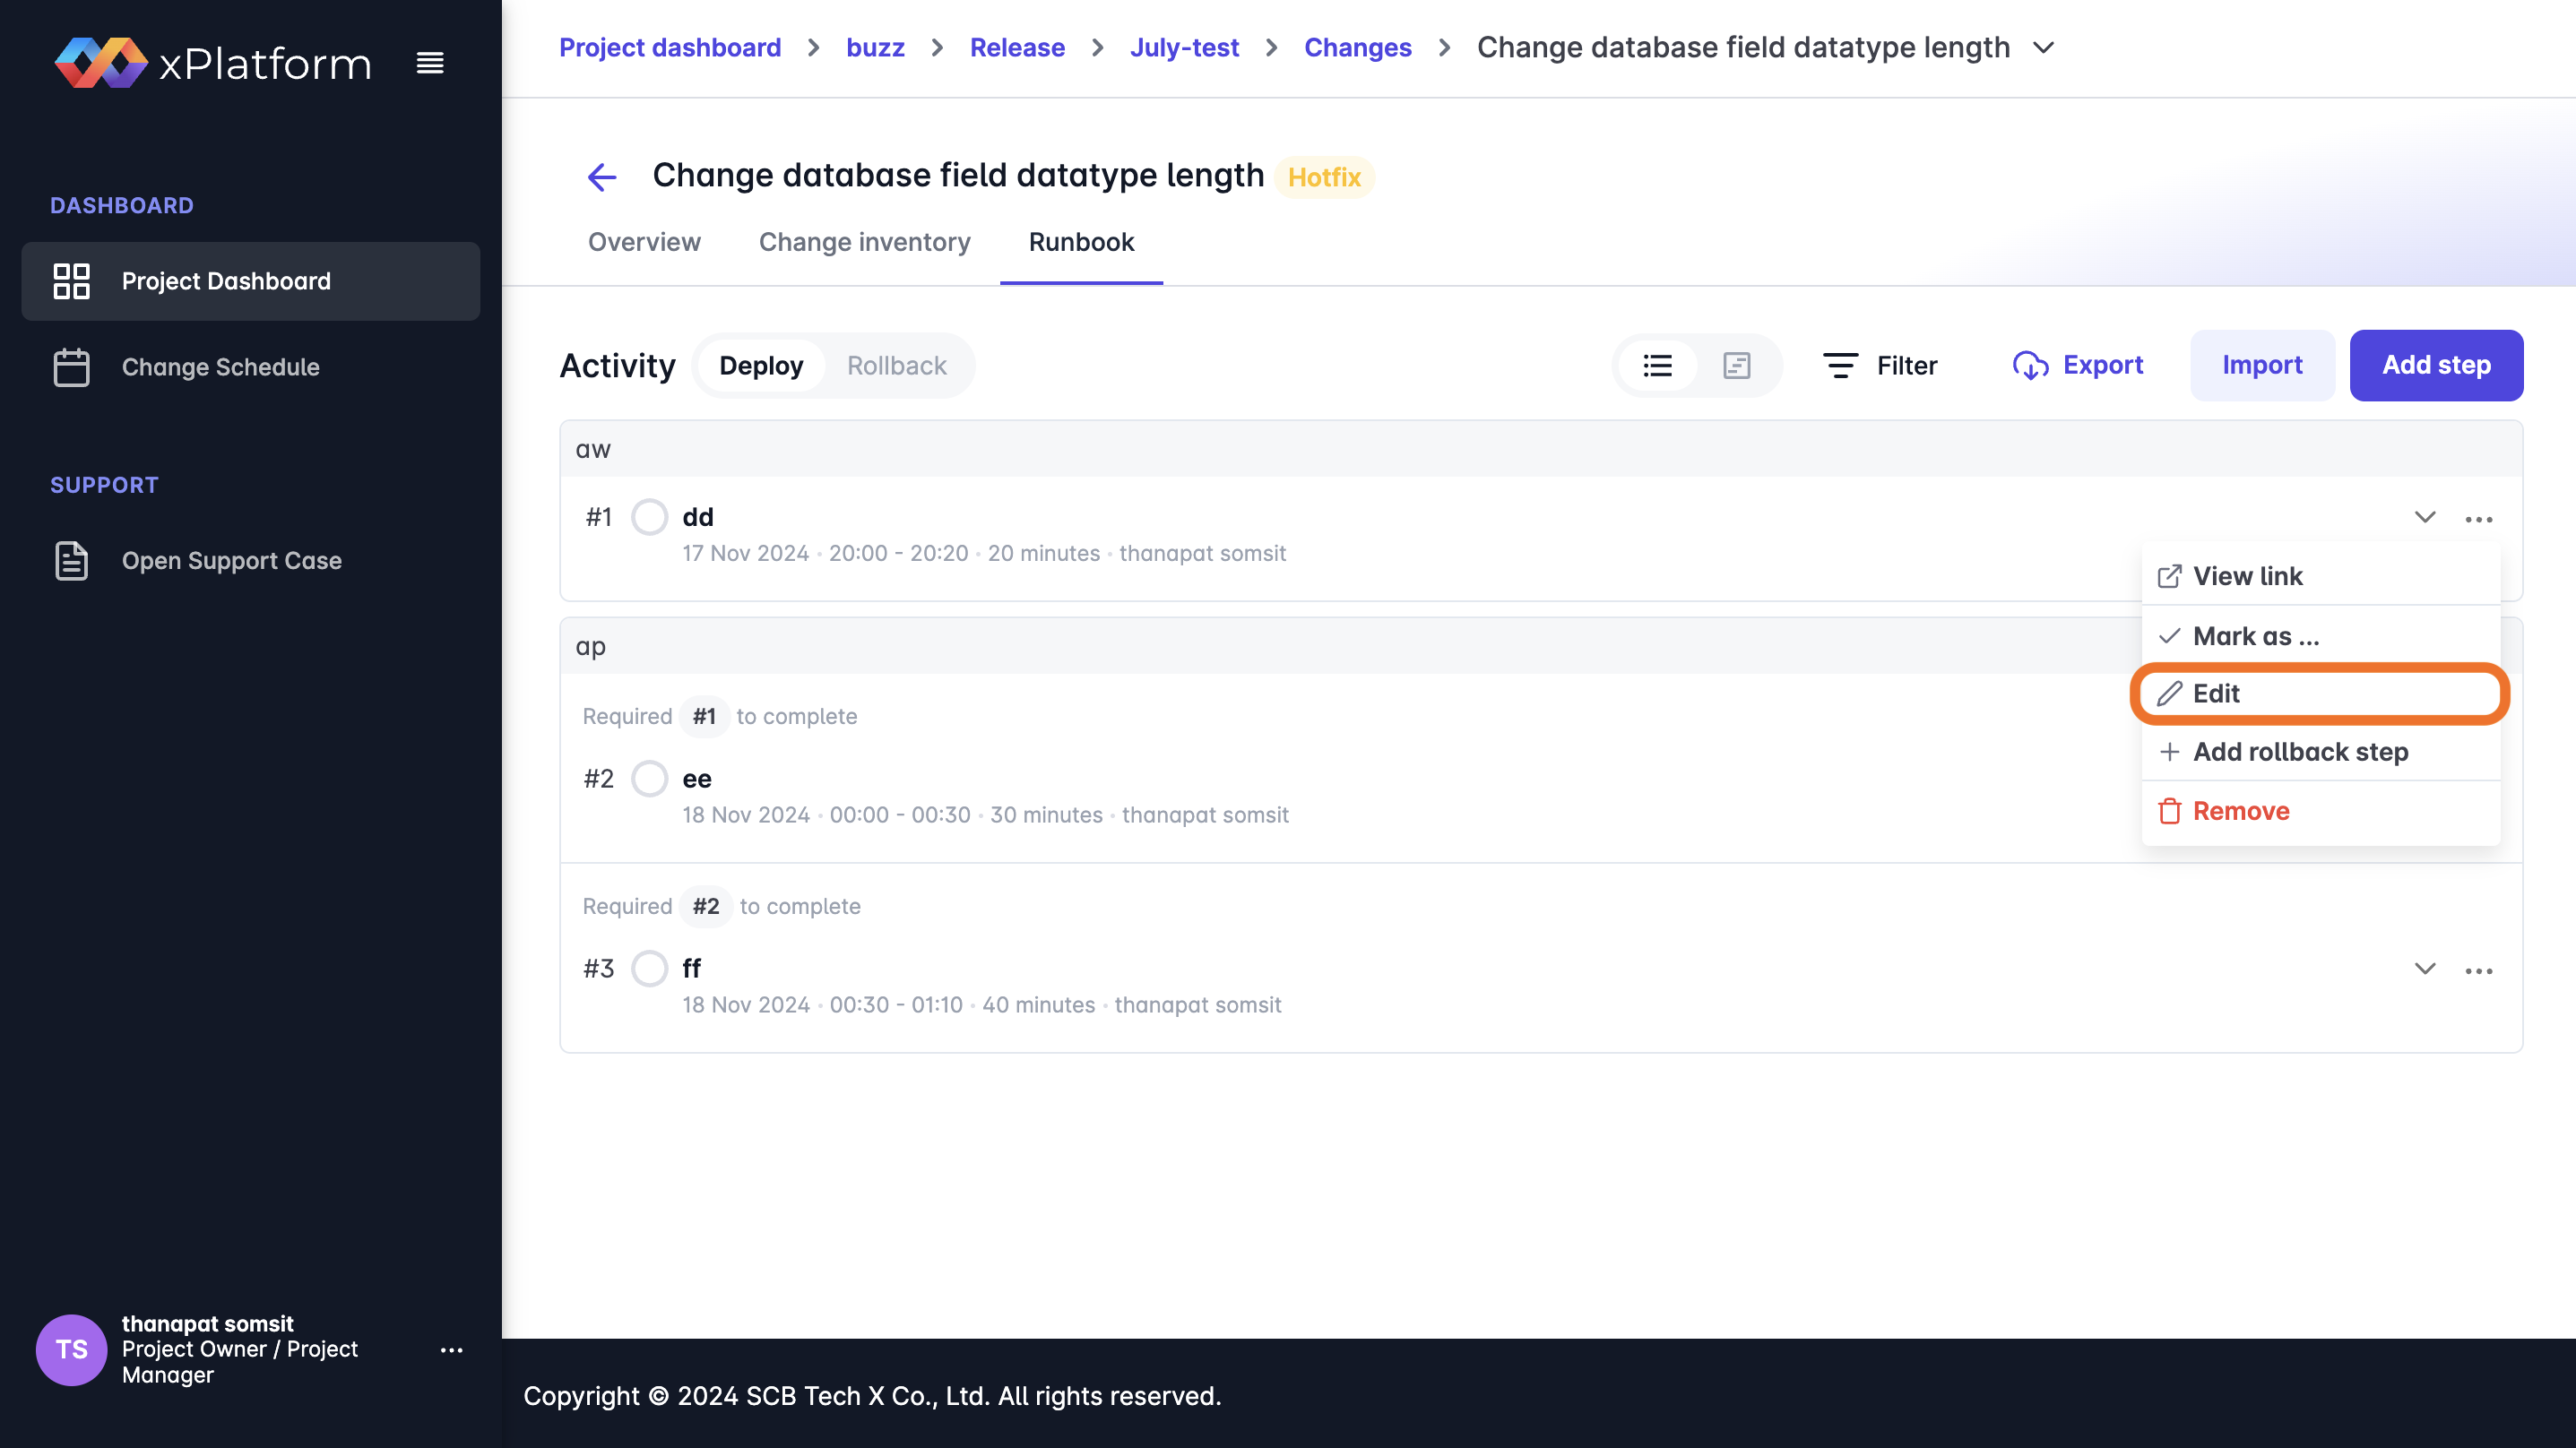
\includegraphics[width=\linewidth]{resources/pages/change-runbook/update-activity/8.png}
\end{center}

\begin{figure}[H]
\begin{center}
    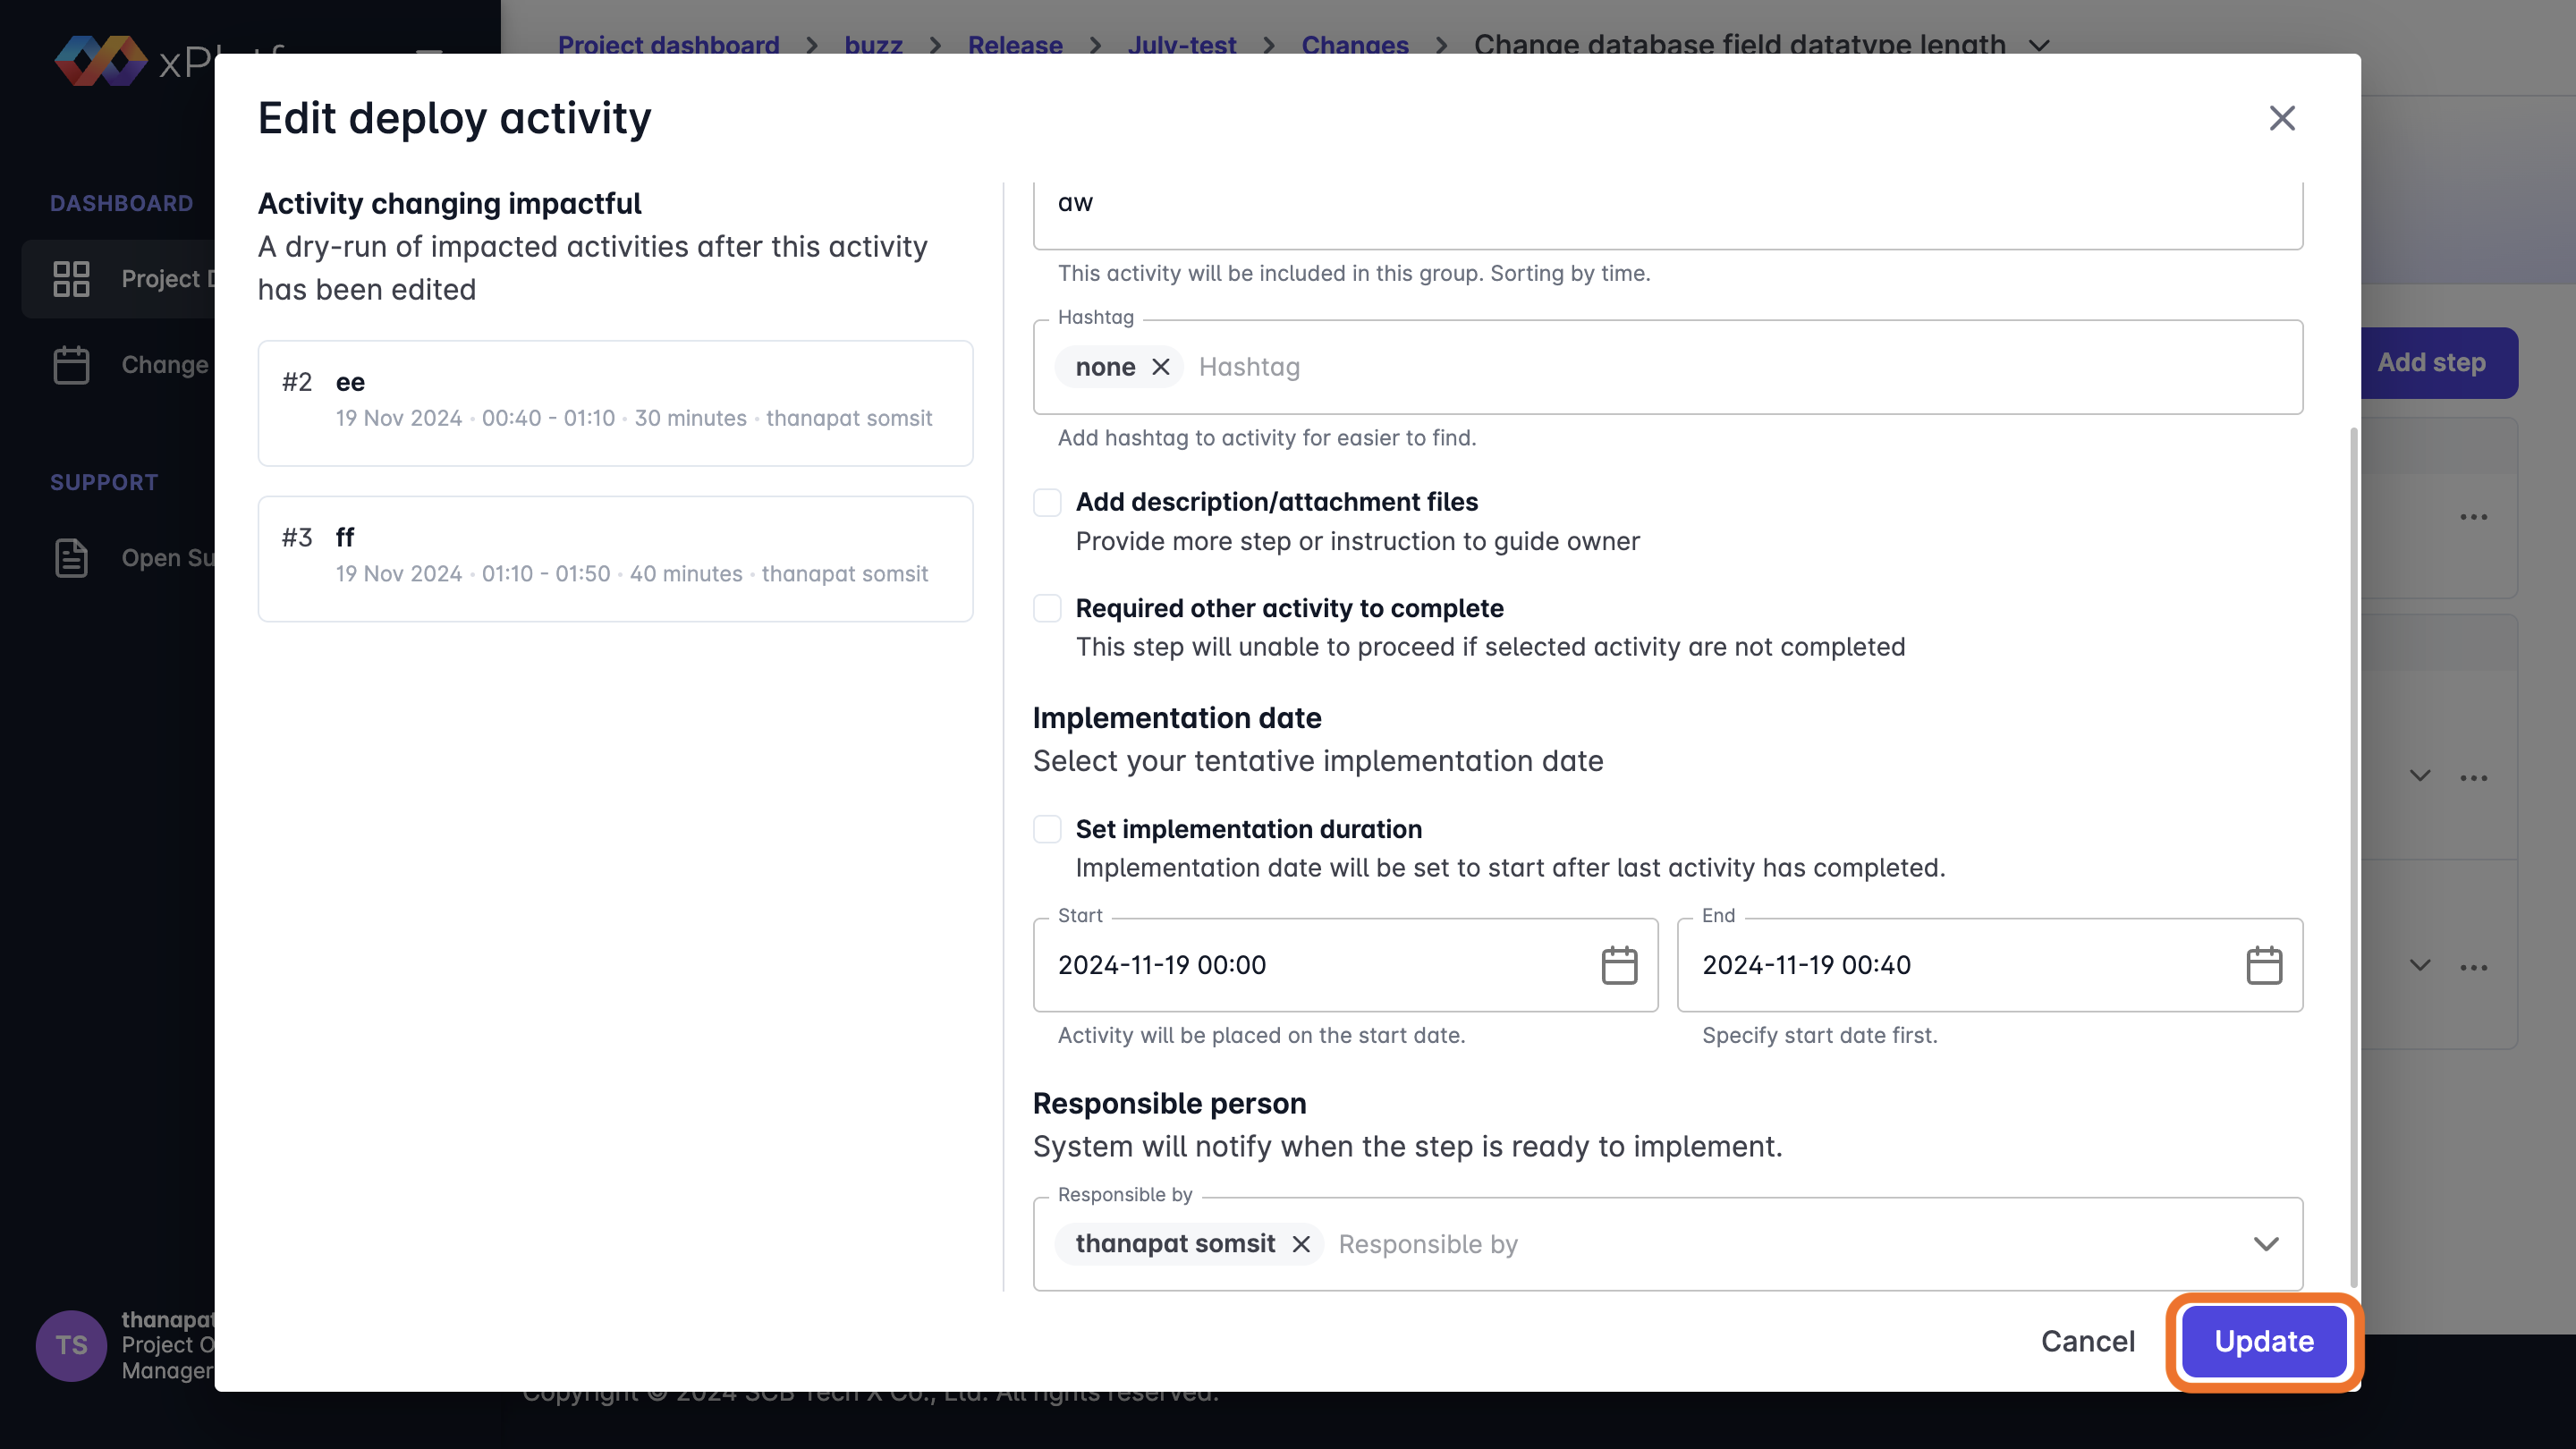
\includegraphics[width=\linewidth]{resources/pages/change-runbook/update-activity/9.png}

    \vspace{1in}

    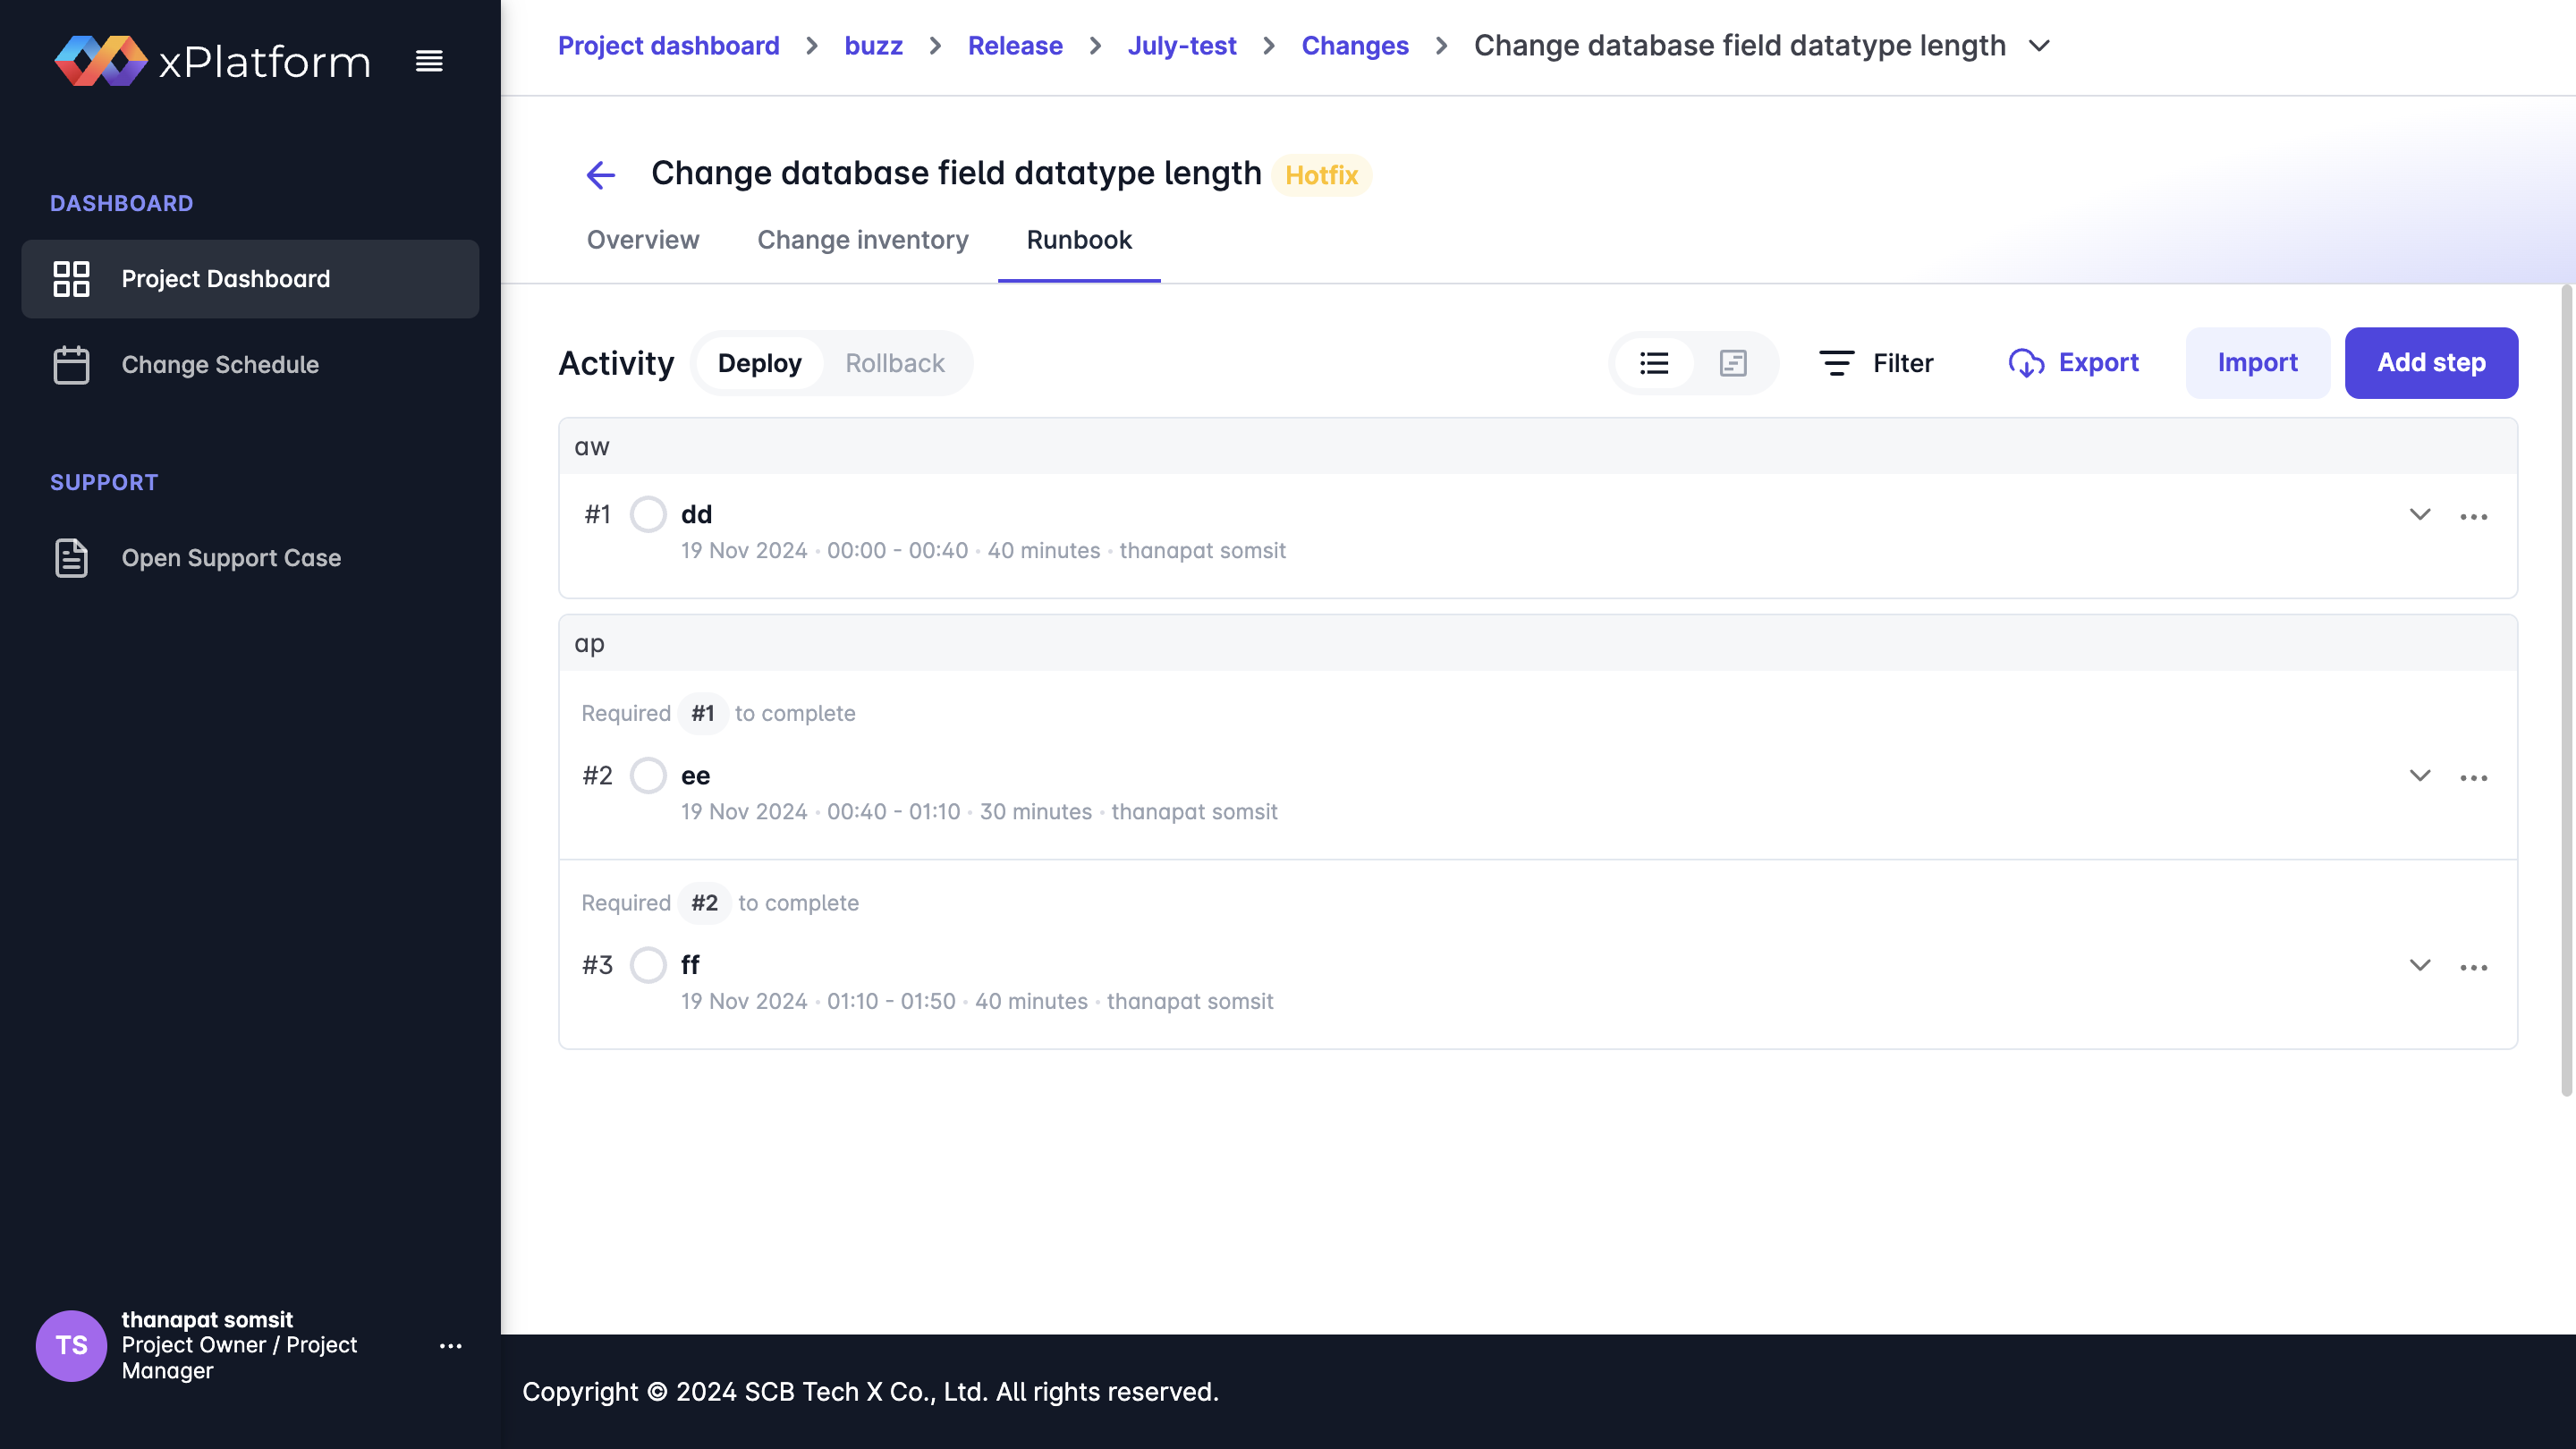
\includegraphics[width=\linewidth]{resources/pages/change-runbook/update-activity/10.png}
\end{center}
\caption[การเปลี่ยนแปลง Activity]{การเปลี่ยนแปลง Activity}
\label{fig:update-activity}
\end{figure}

\newpage
\subsection{การลบ Activity}
\begin{center}
    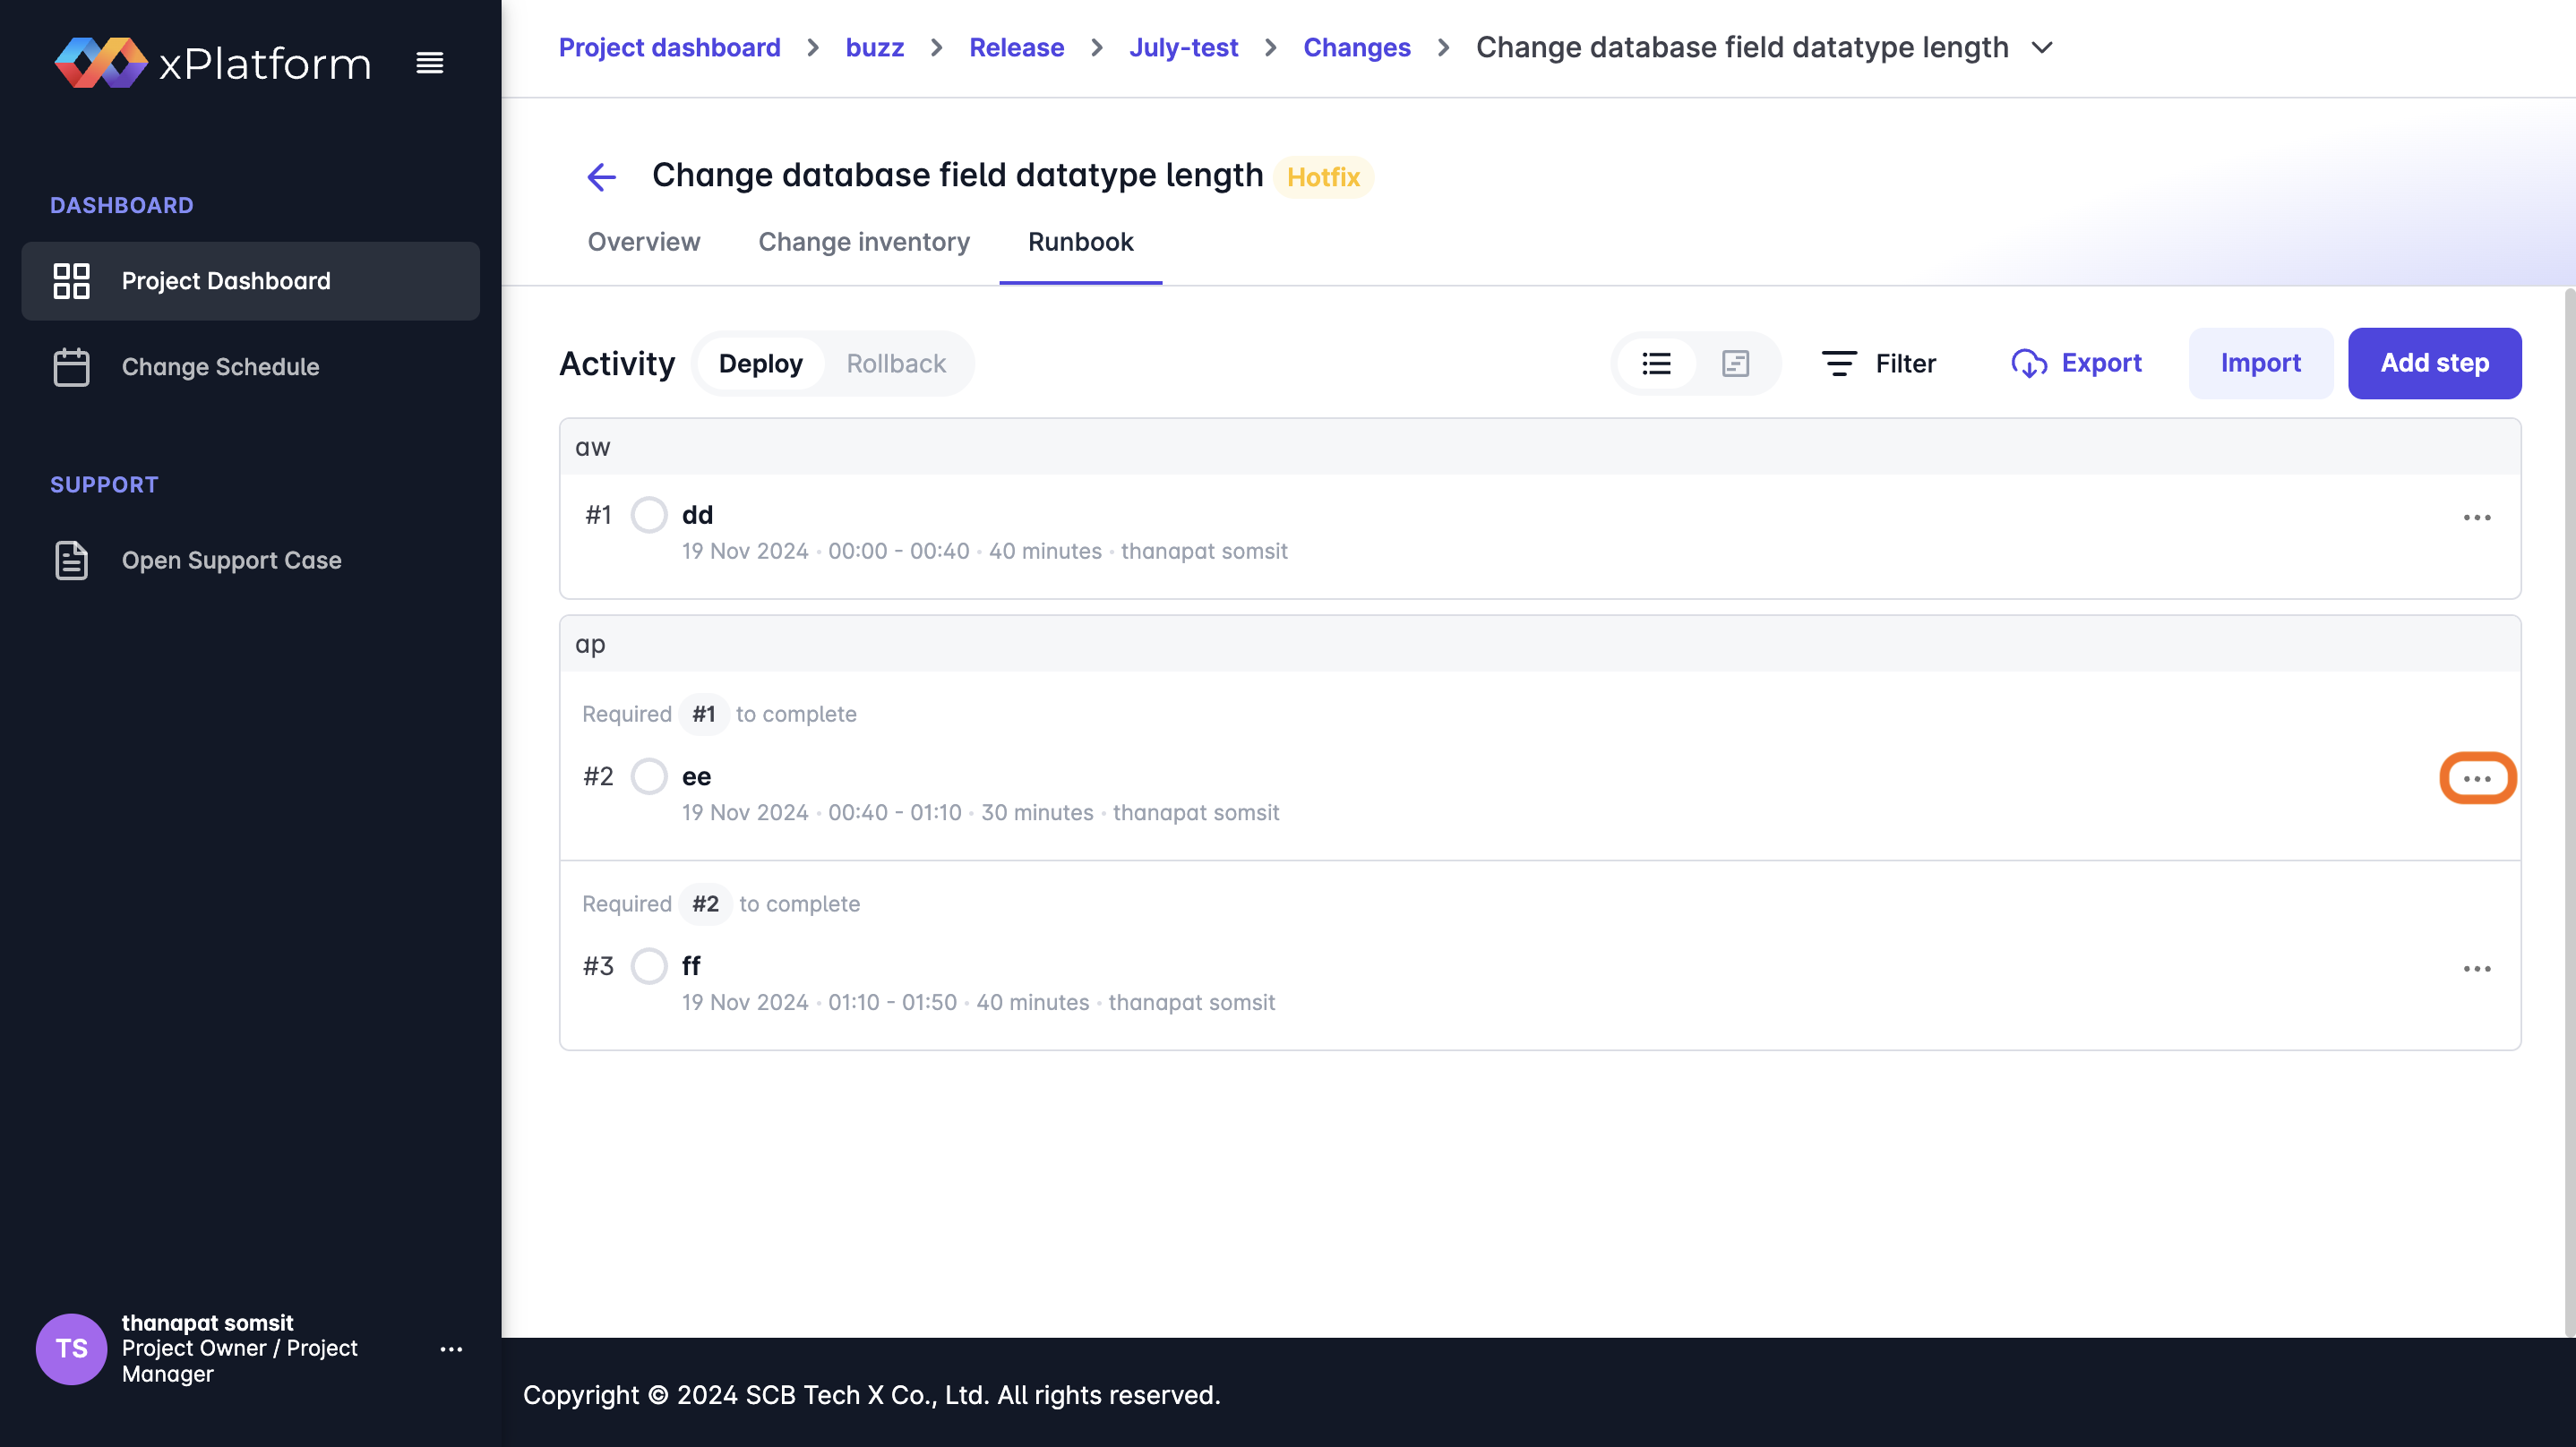
\includegraphics[width=\linewidth]{resources/pages/change-runbook/delete-activity/41.png}
    
    \vspace{1in}
    
    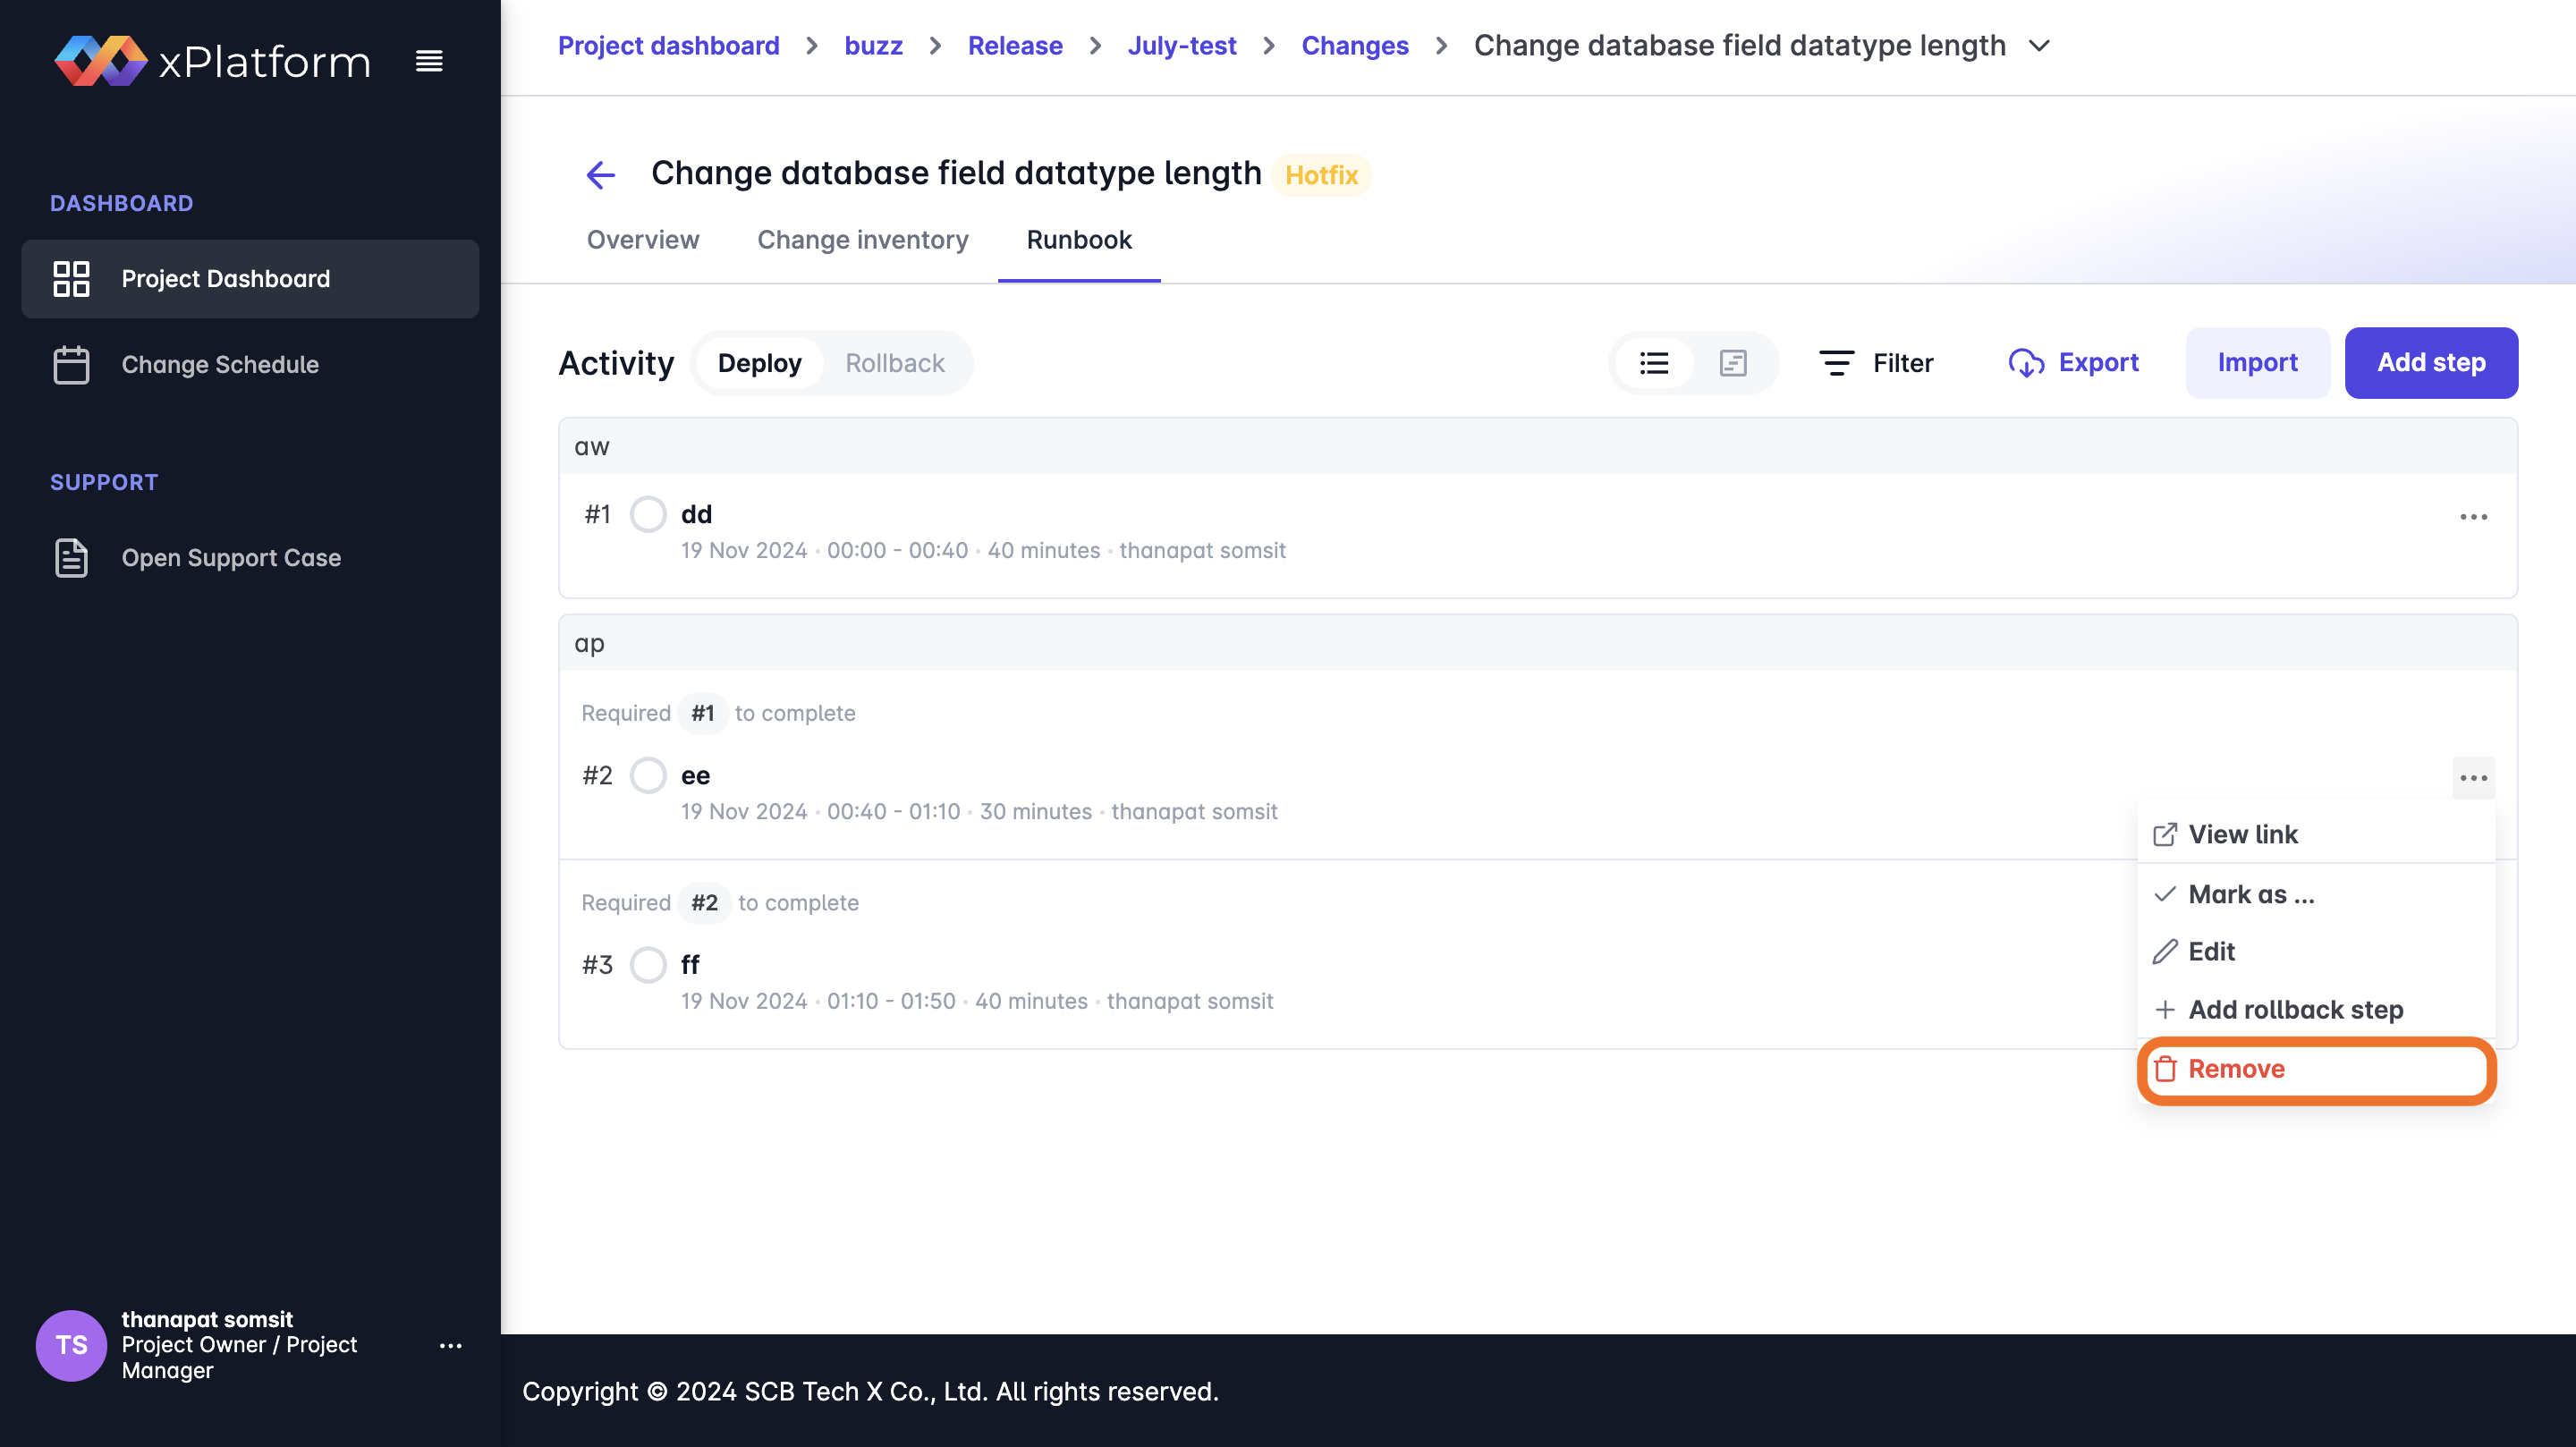
\includegraphics[width=\linewidth]{resources/pages/change-runbook/delete-activity/42.png}
\end{center}
    
\begin{figure}[H]
\begin{center}
    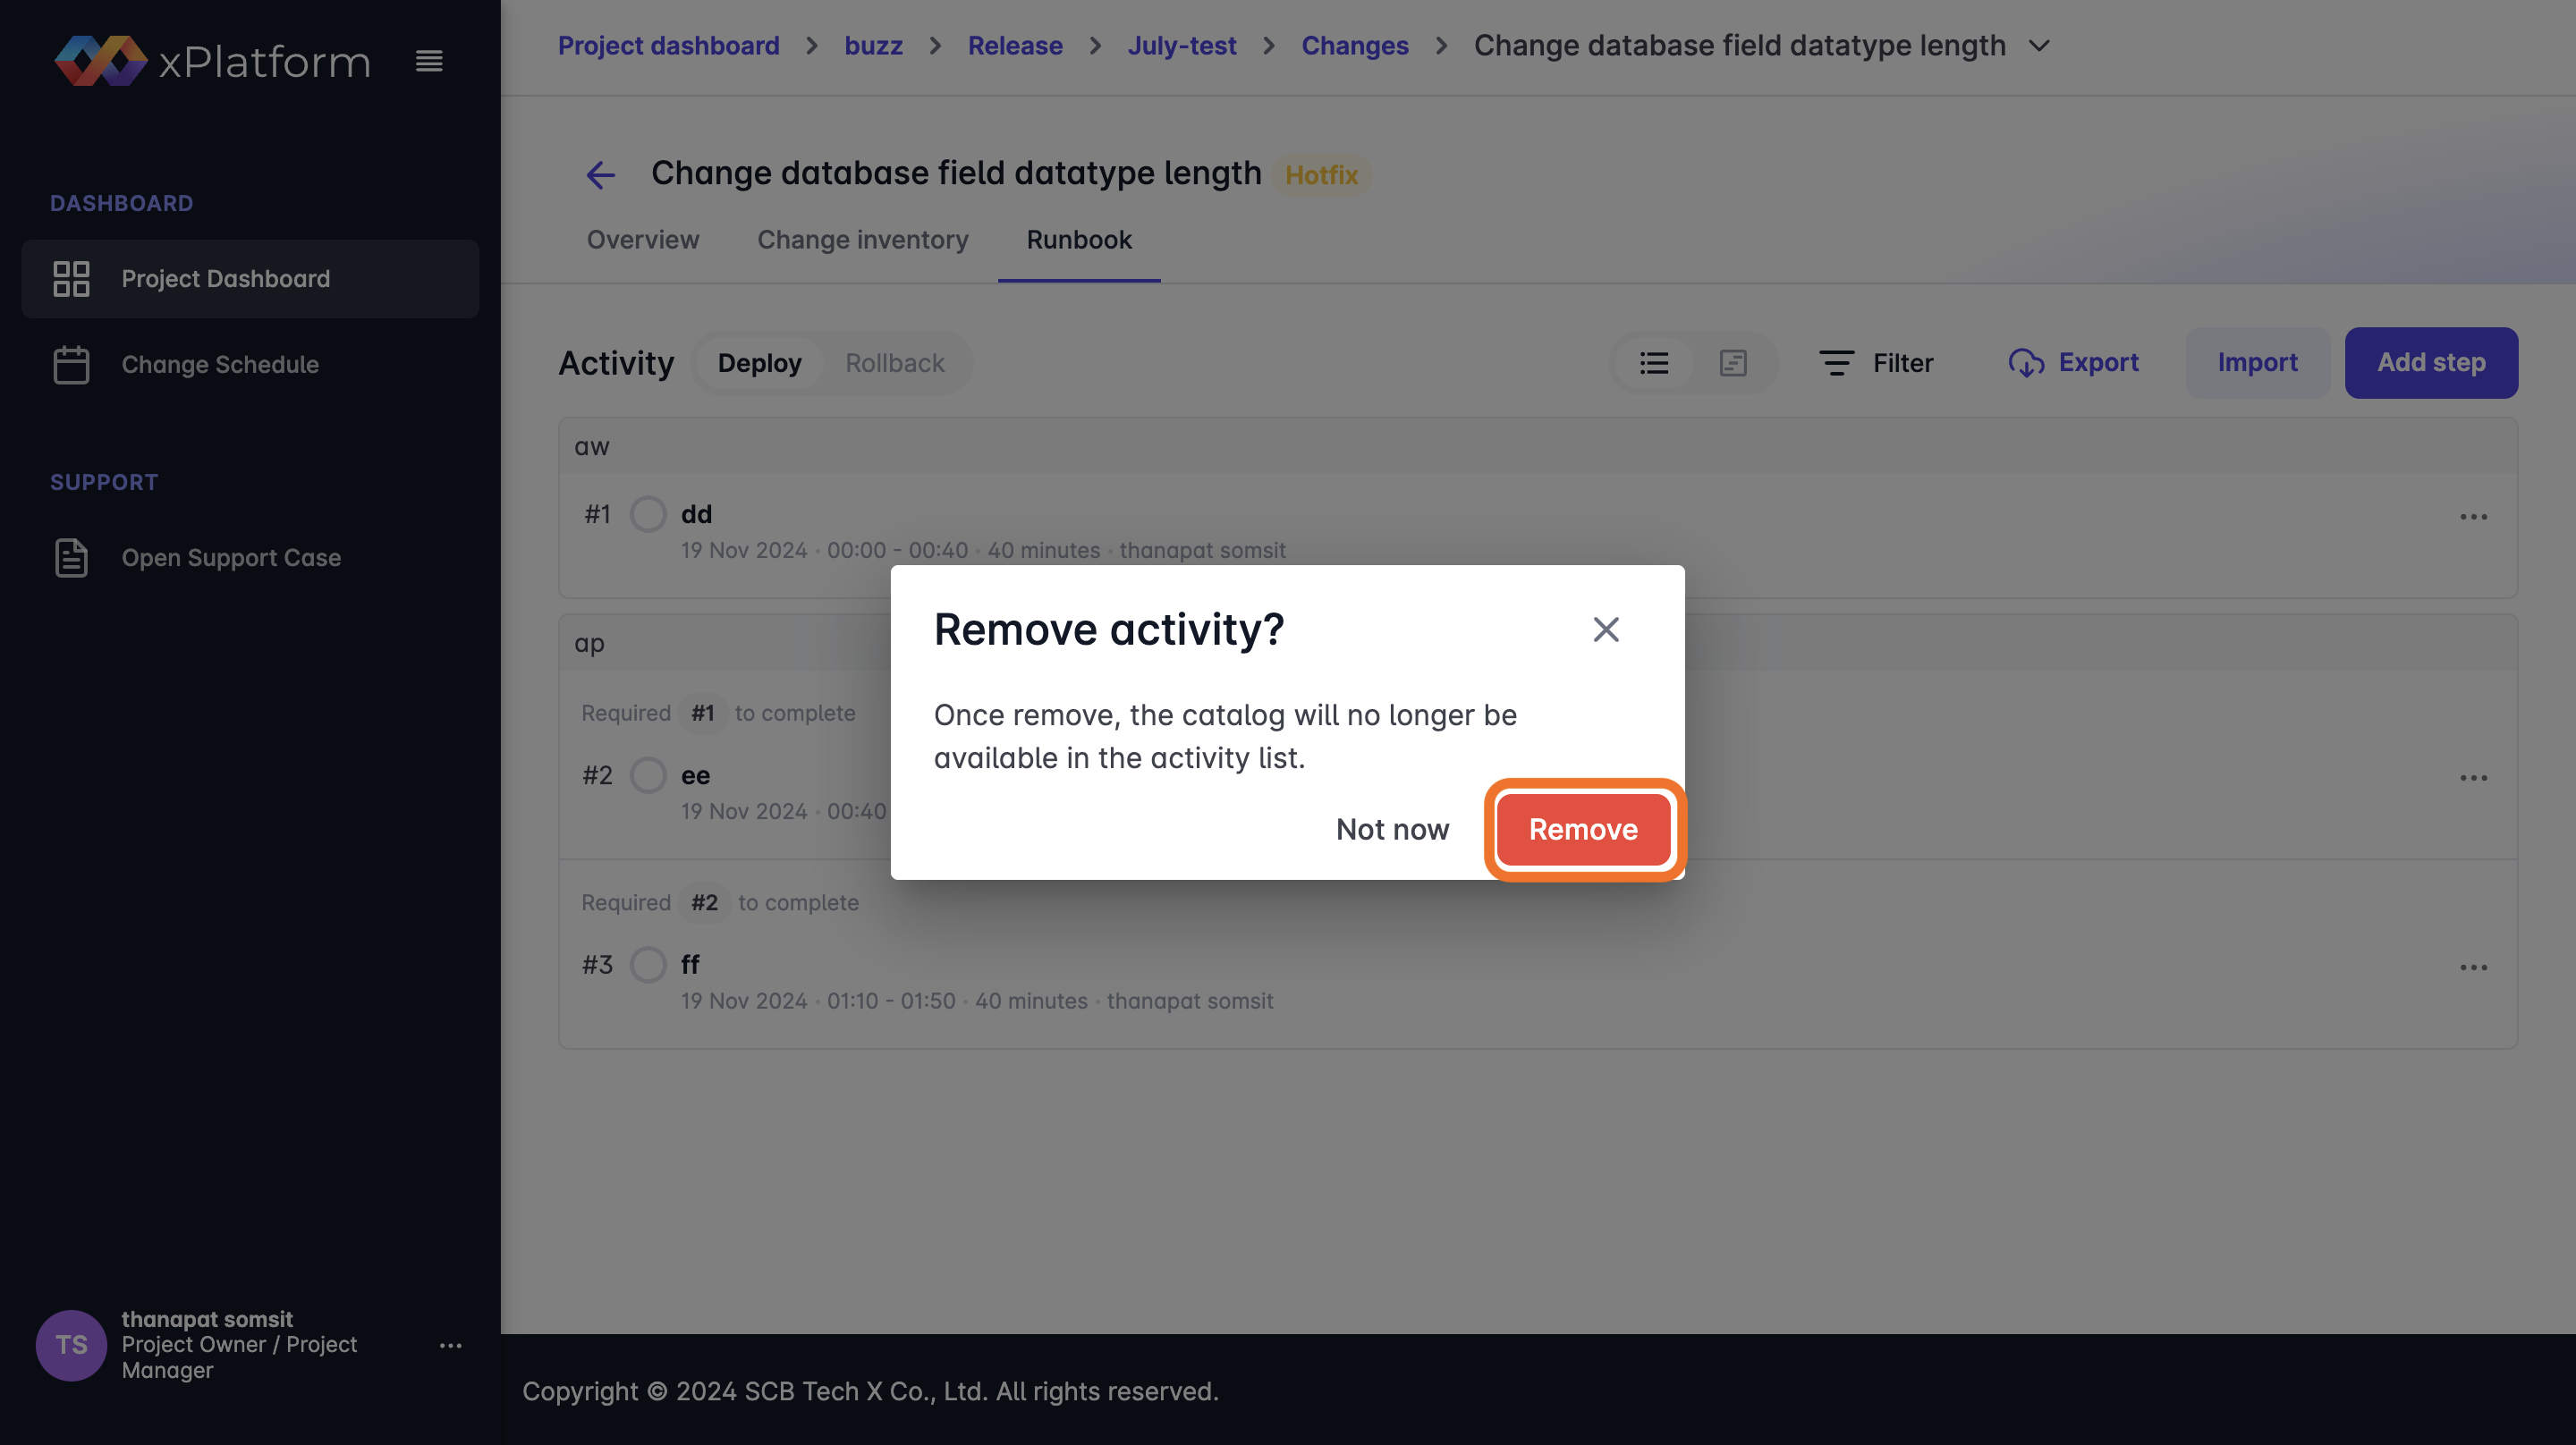
\includegraphics[width=\linewidth]{resources/pages/change-runbook/delete-activity/43.png}

    \vspace{1in}

    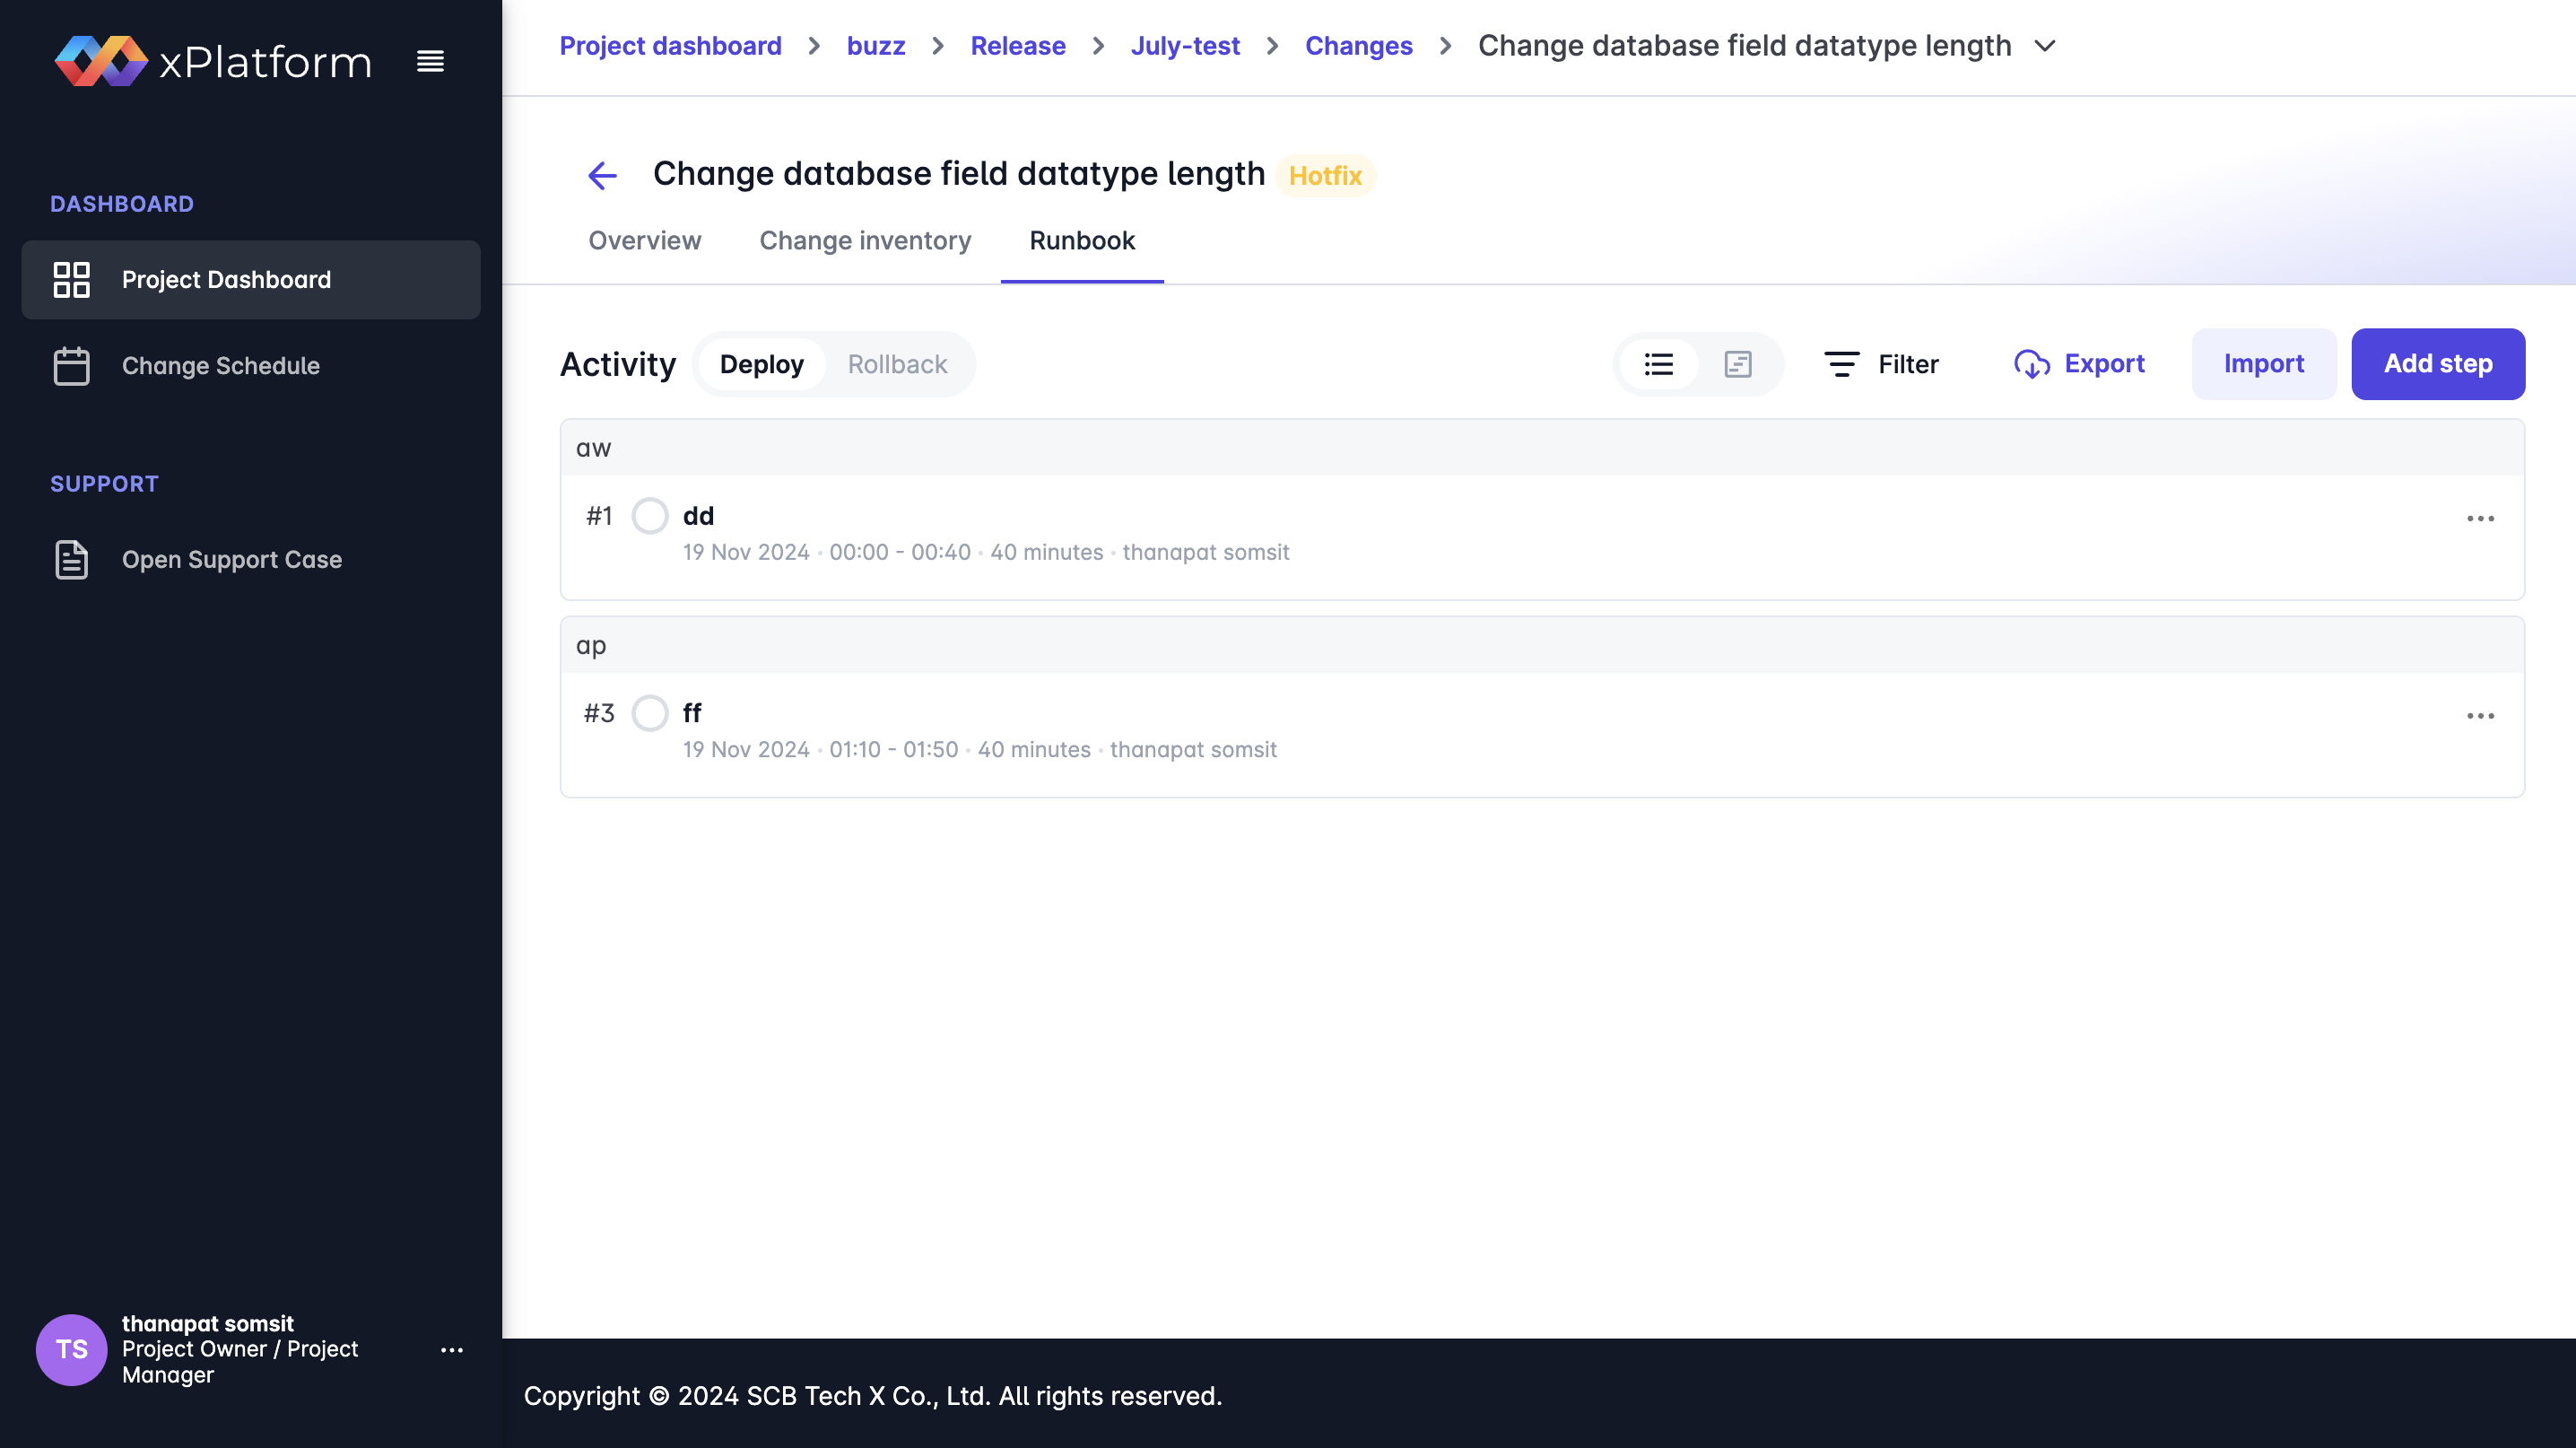
\includegraphics[width=\linewidth]{resources/pages/change-runbook/delete-activity/44.png}
\end{center}
\caption[การลบ Activity]{การลบ Activity}
\label{fig:delete-activity}
\end{figure}

\newpage
\subsection{การ Mark Activity}
\begin{center}
    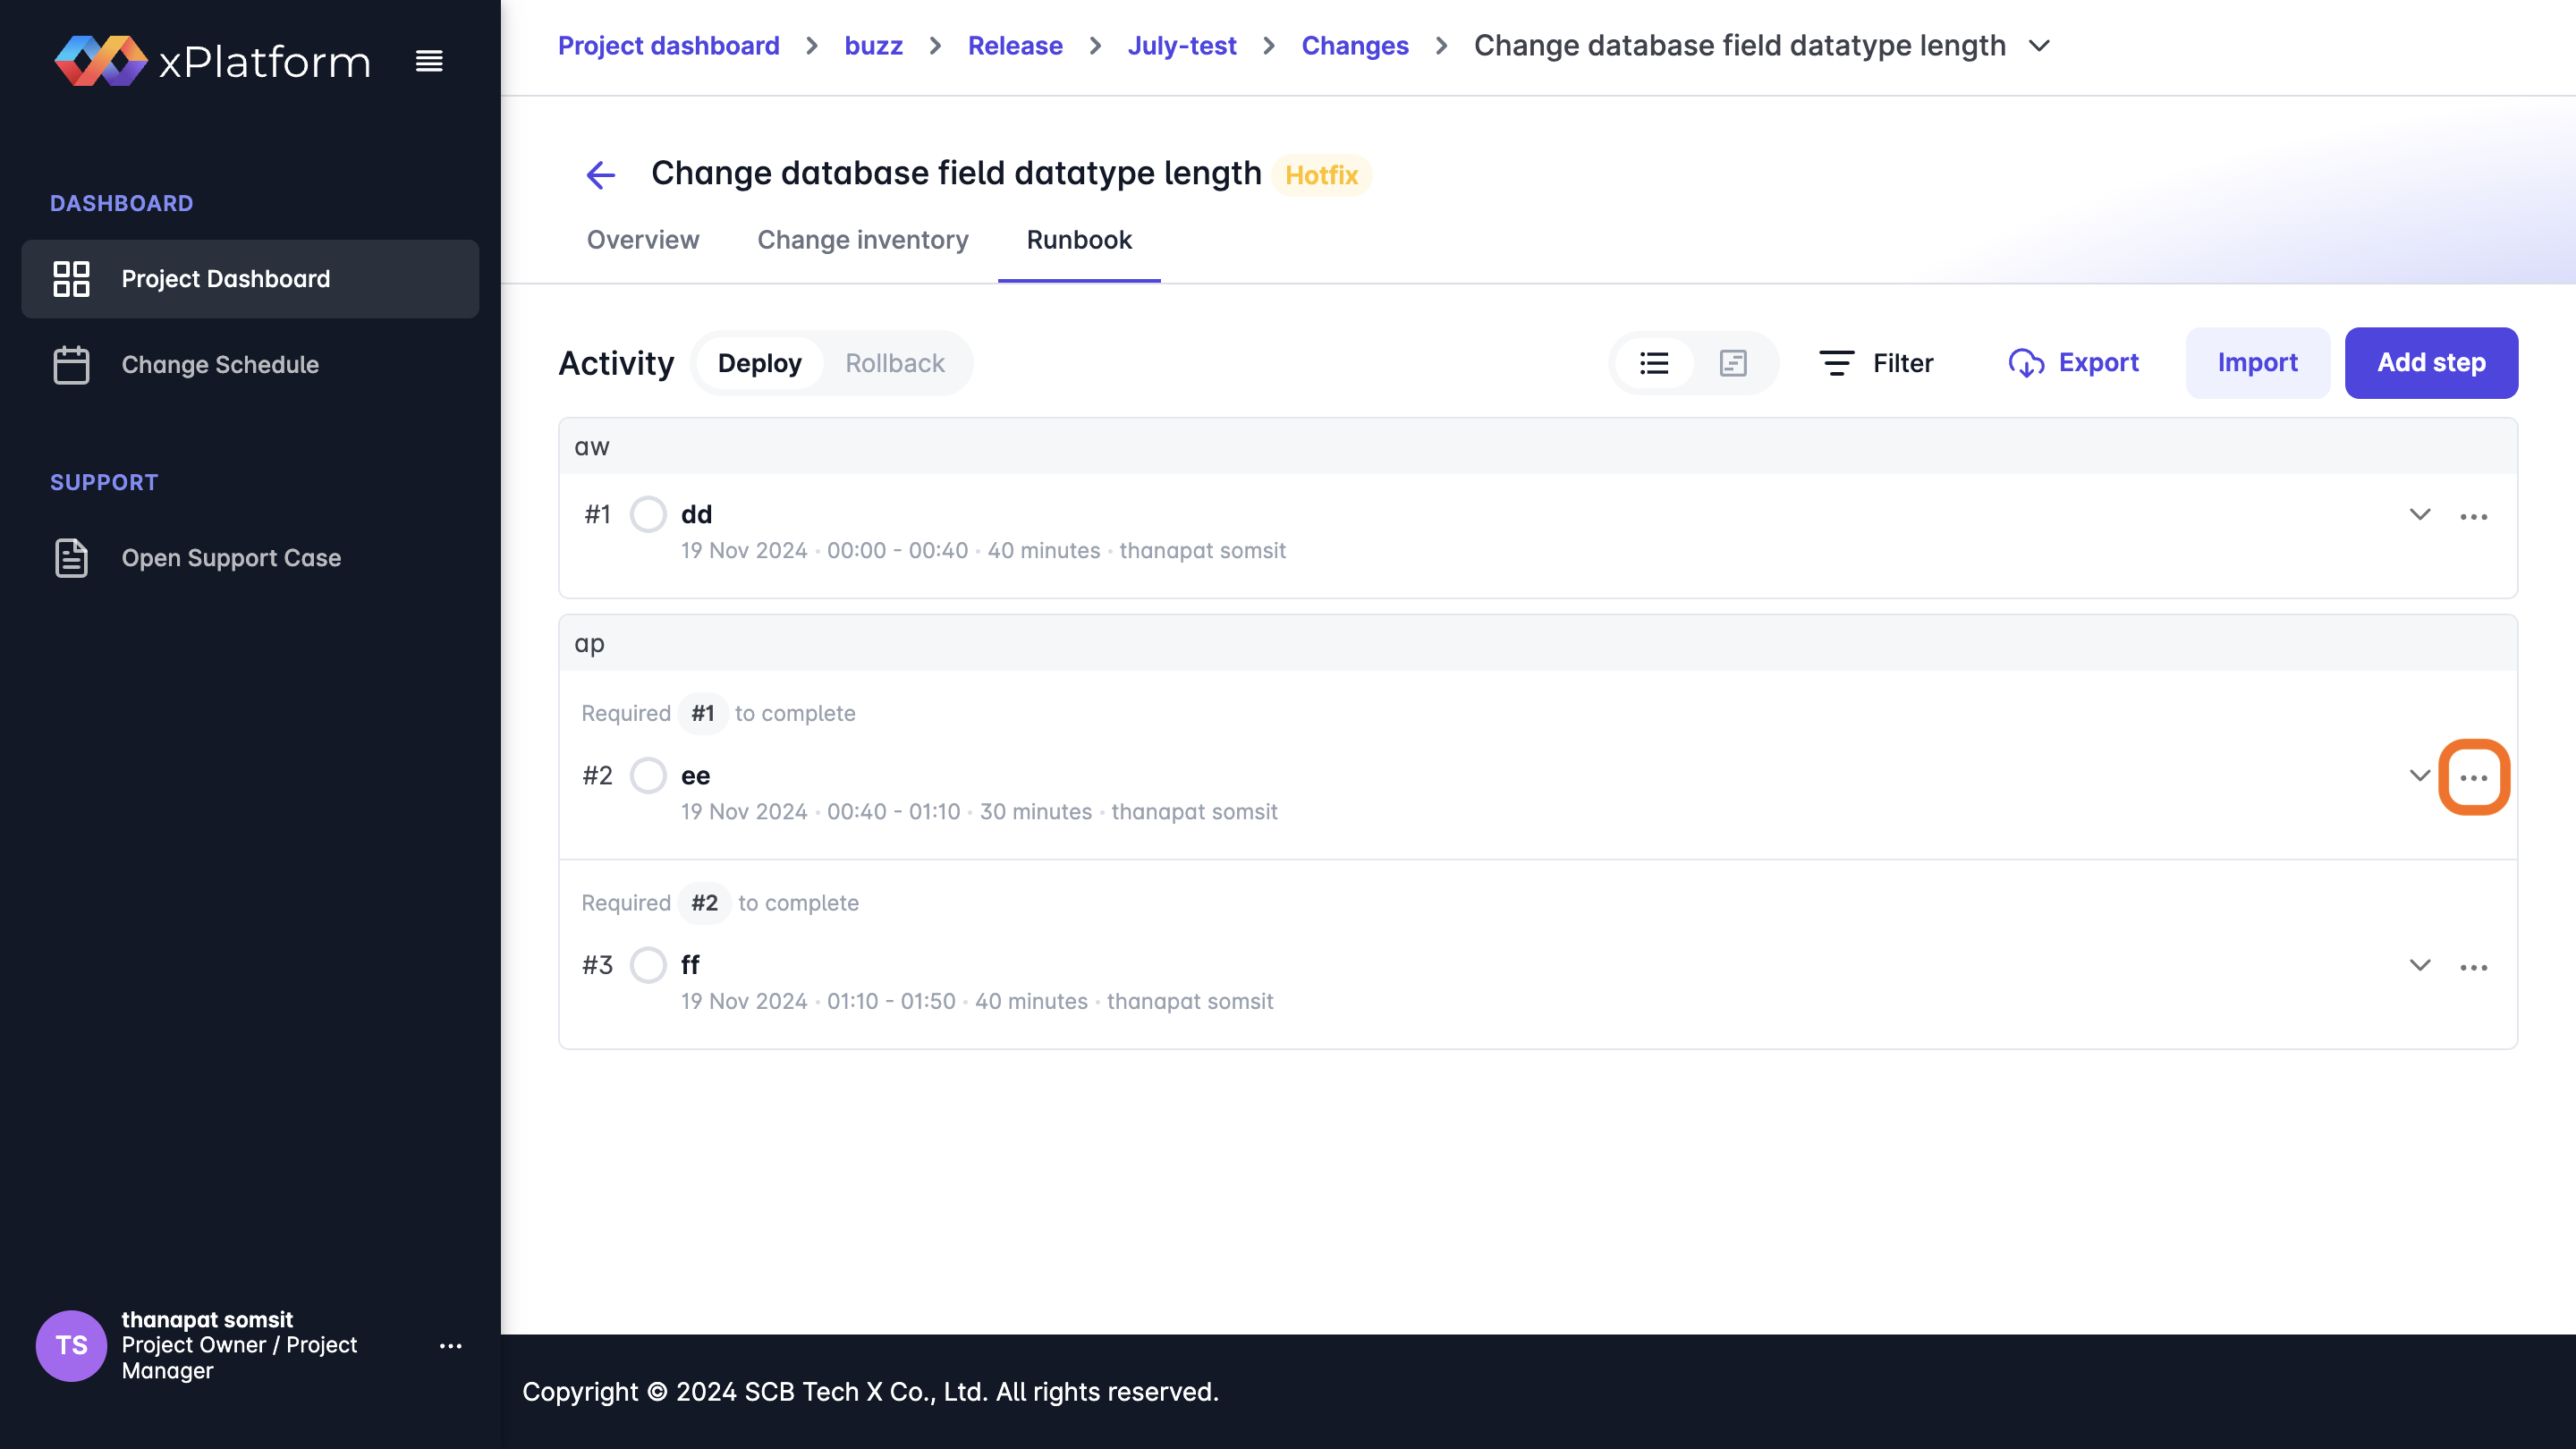
\includegraphics[width=\linewidth]{resources/pages/change-runbook/mark-activity/13.png}
    
    \vspace{1in}
    
    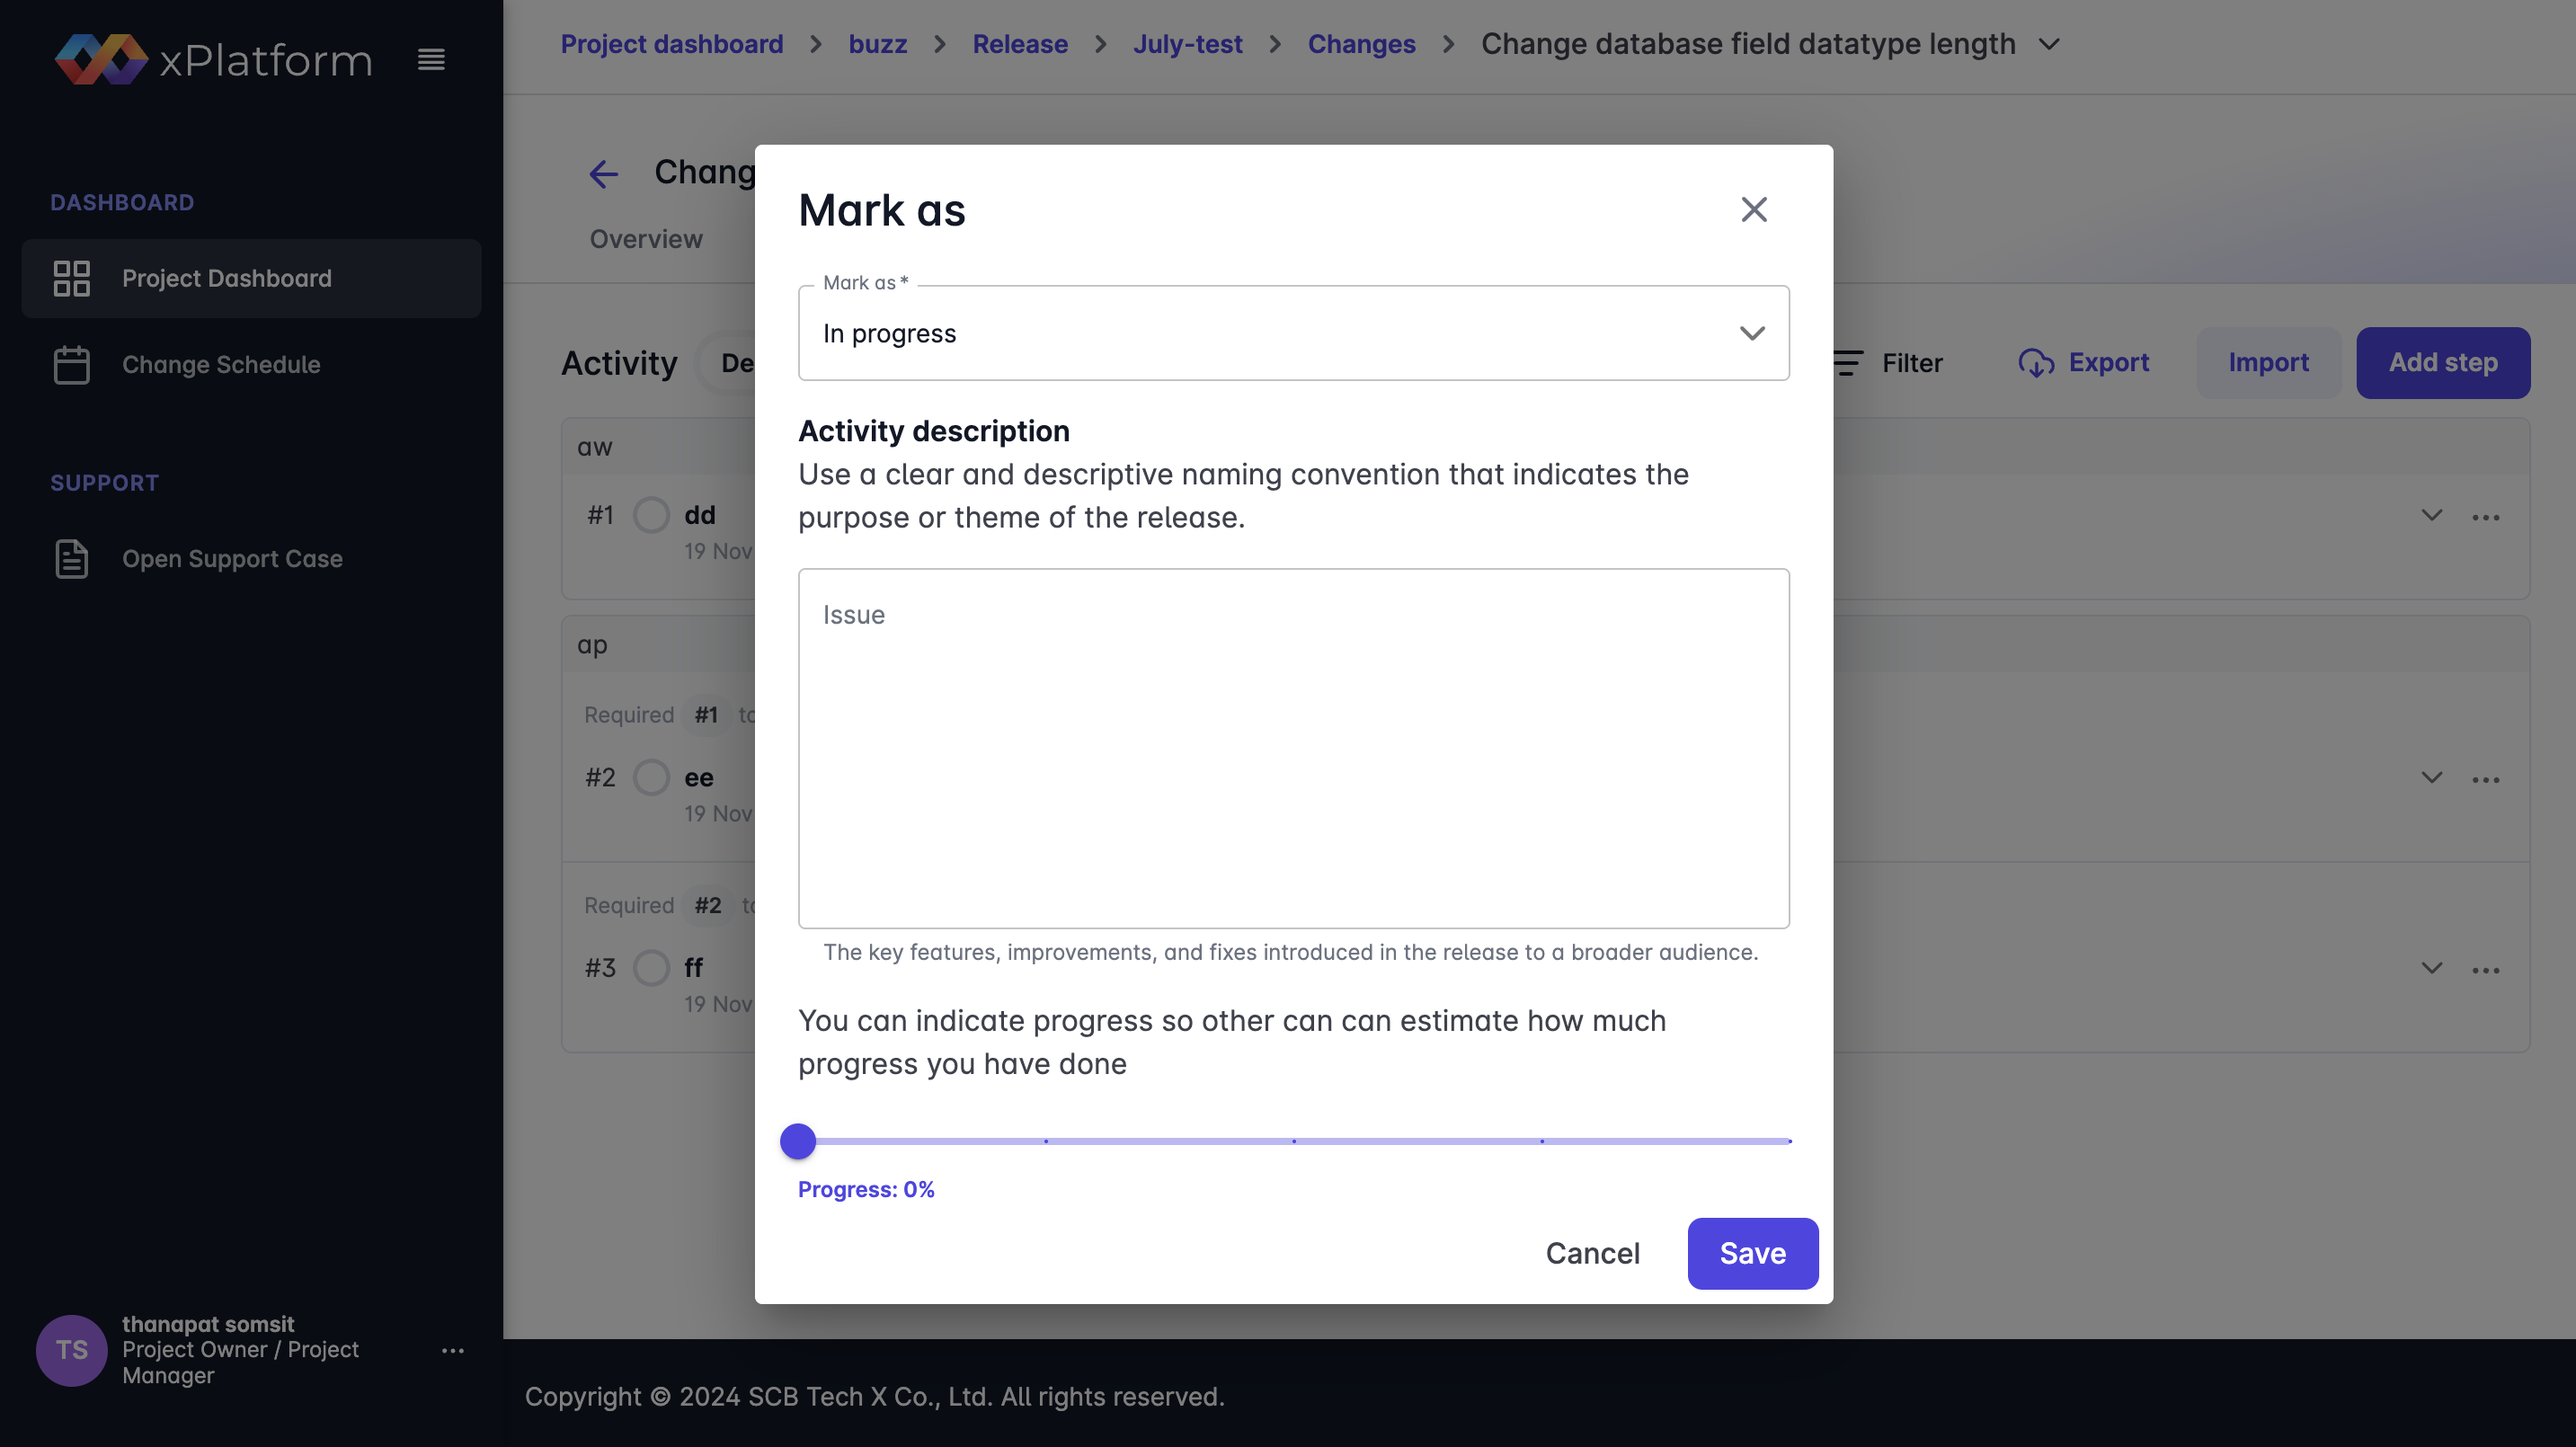
\includegraphics[width=\linewidth]{resources/pages/change-runbook/mark-activity/14.png}
\end{center}
    
\begin{figure}[H]
\begin{center}
    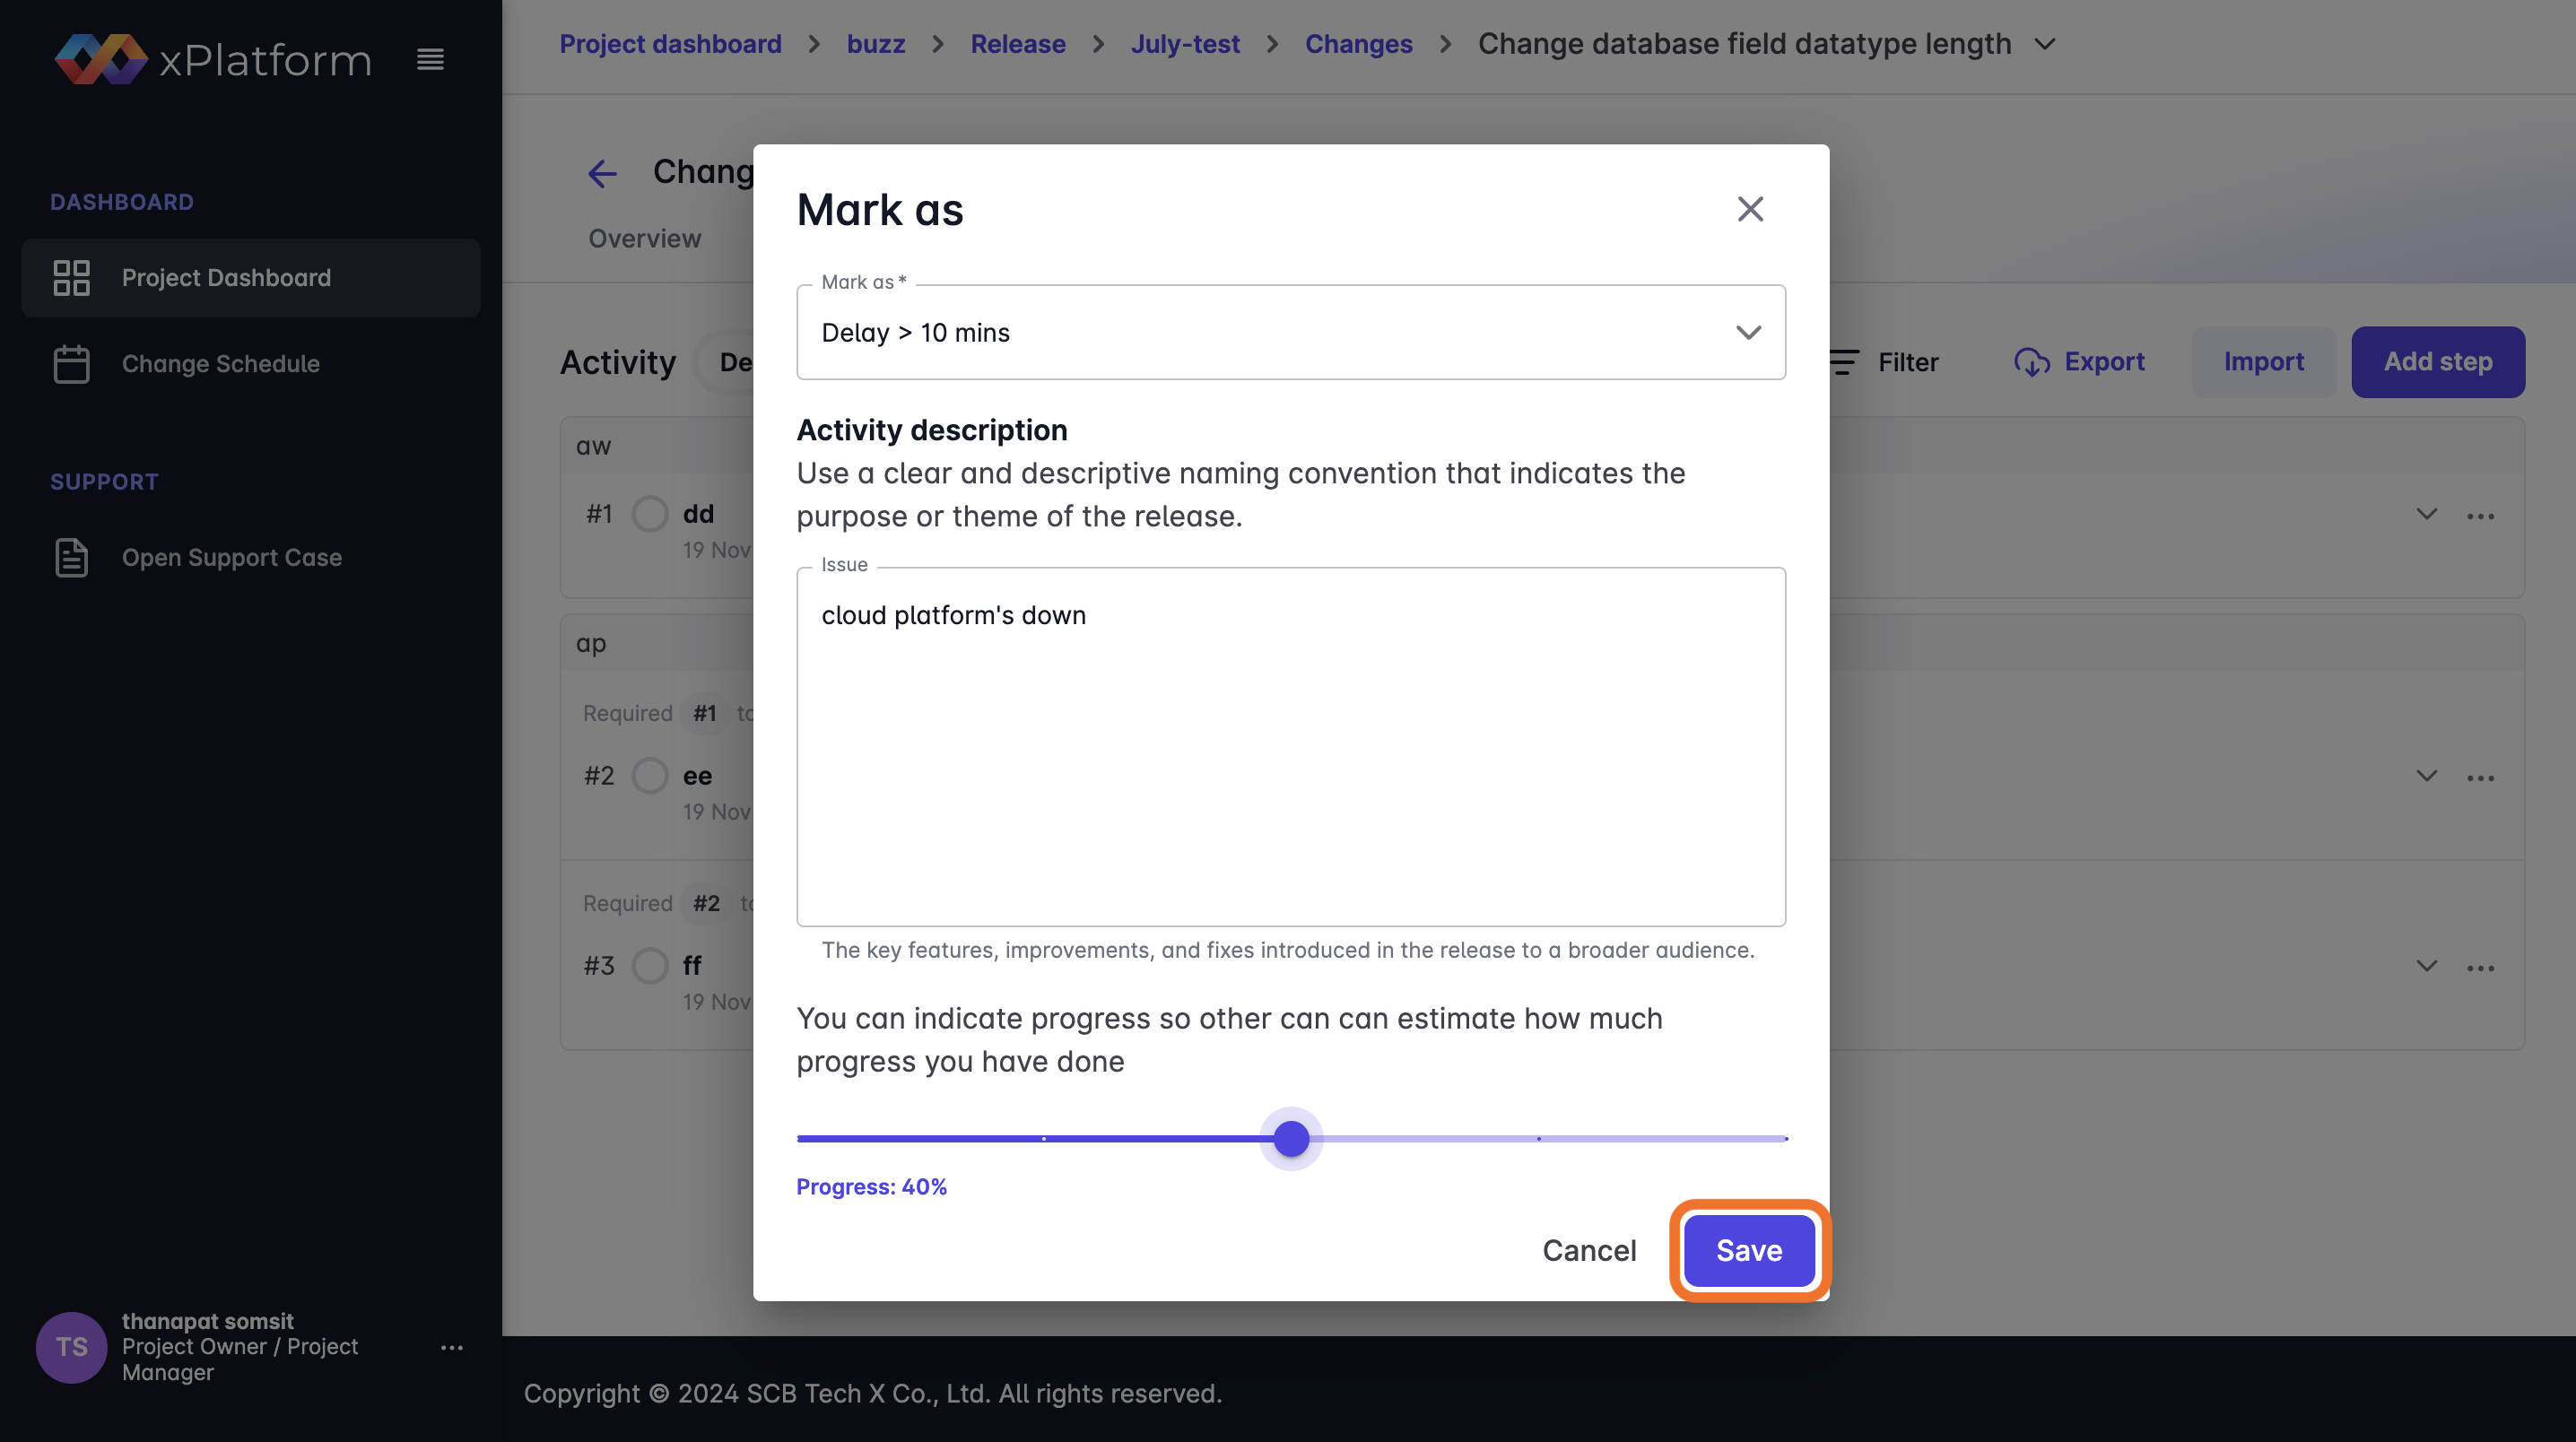
\includegraphics[width=\linewidth]{resources/pages/change-runbook/mark-activity/15.png}

    \vspace{1in}

    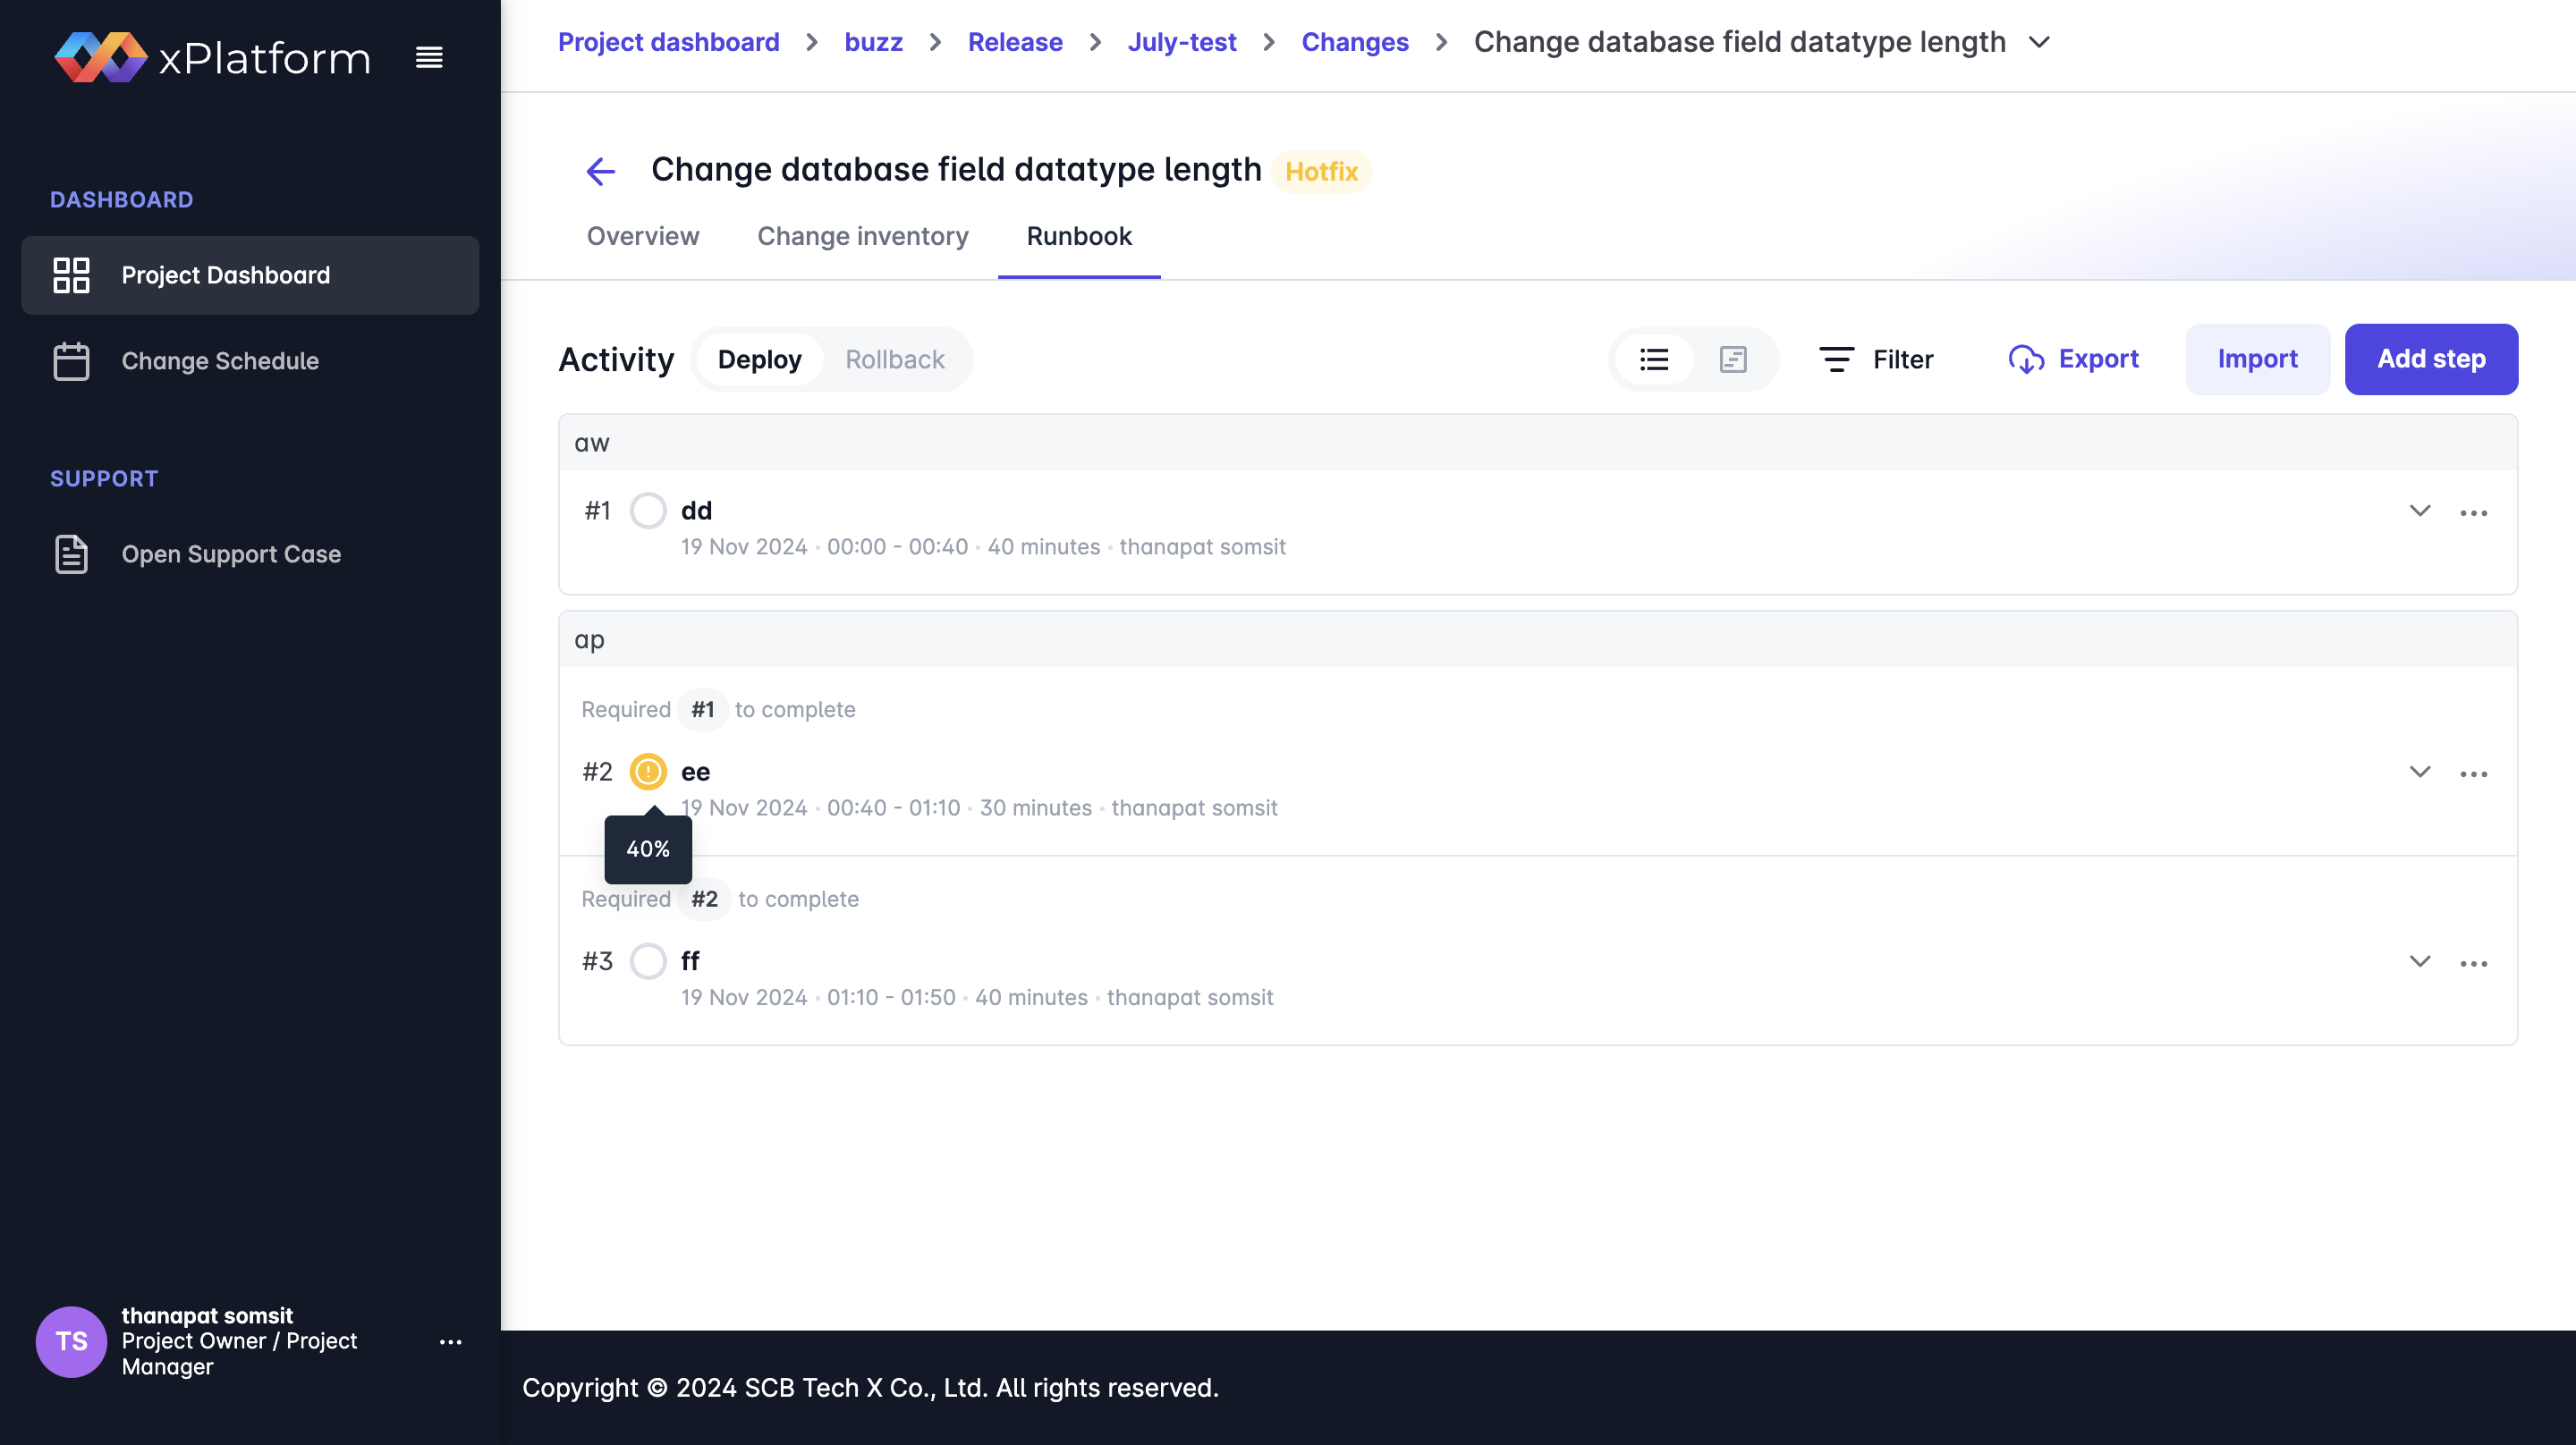
\includegraphics[width=\linewidth]{resources/pages/change-runbook/mark-activity/16.png}
\end{center}
\caption[การ Mark Activity]{การ Mark Activity}
\label{fig:mark-activity}
\end{figure}

\newpage
\subsection{การดึงข้อมูลจาก Jira}
\begin{center}
    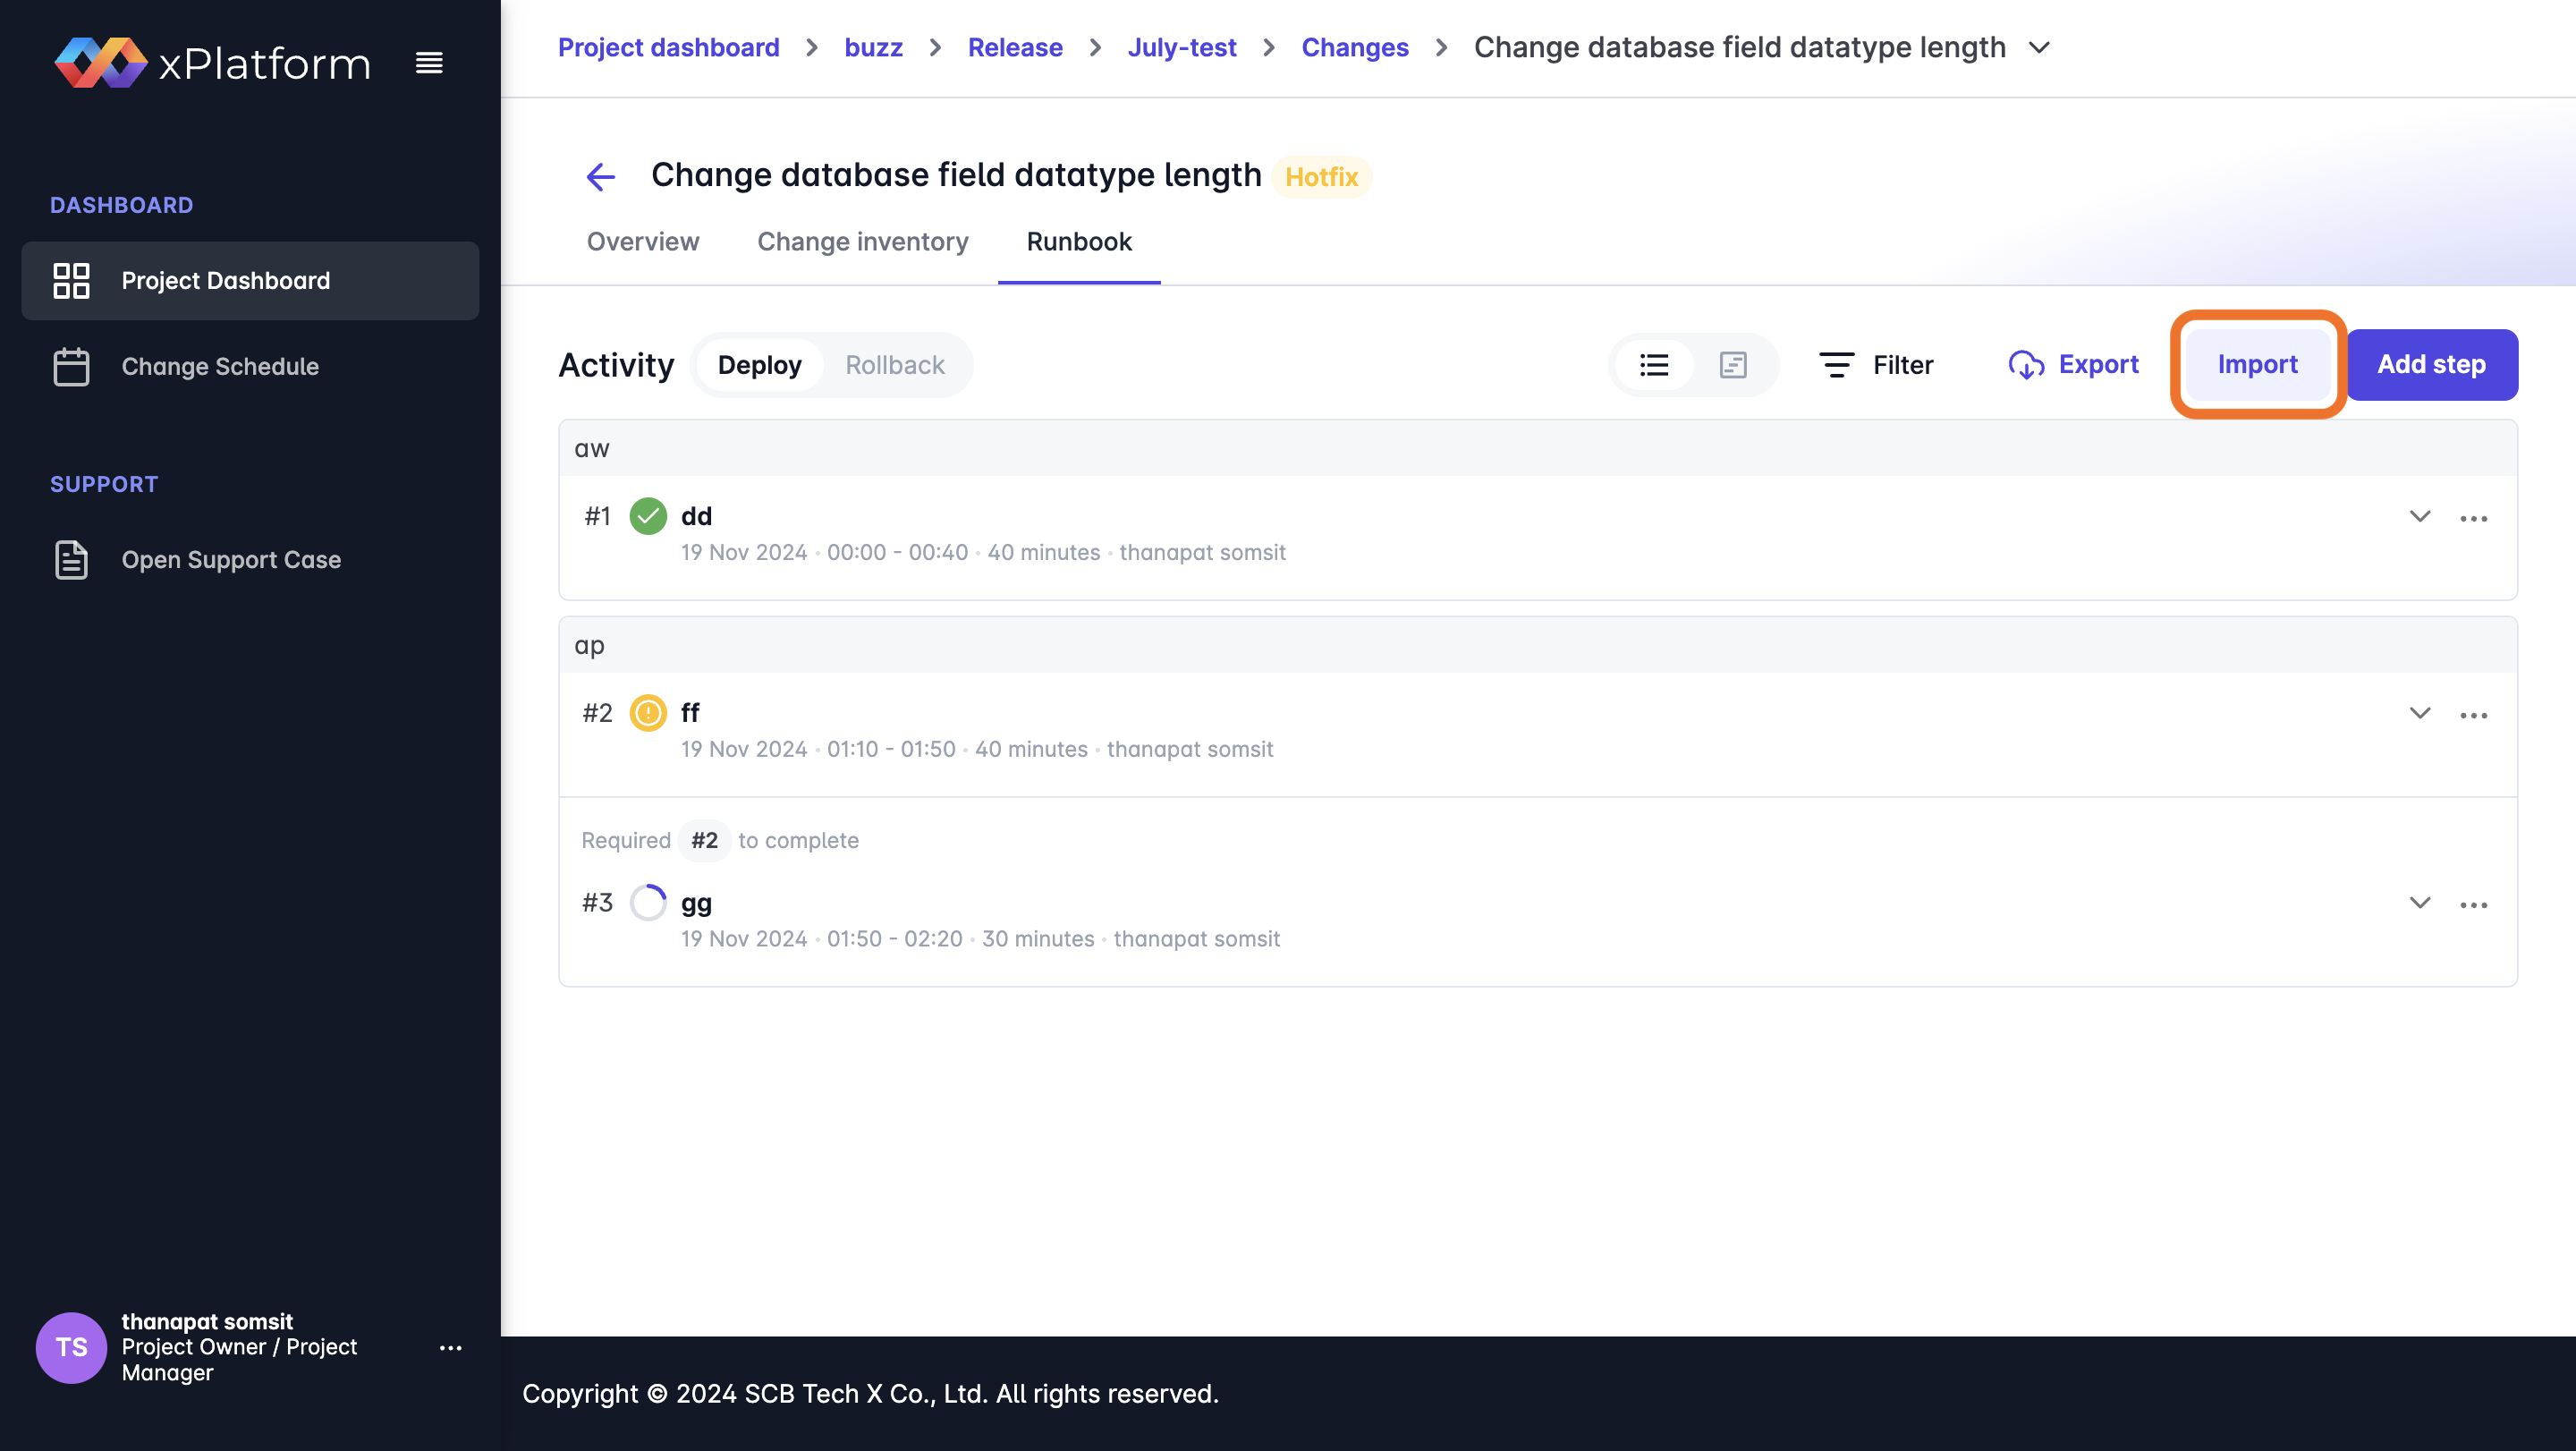
\includegraphics[width=\linewidth]{resources/pages/change-runbook/import-jira/22.png}

    \vspace{1in}

    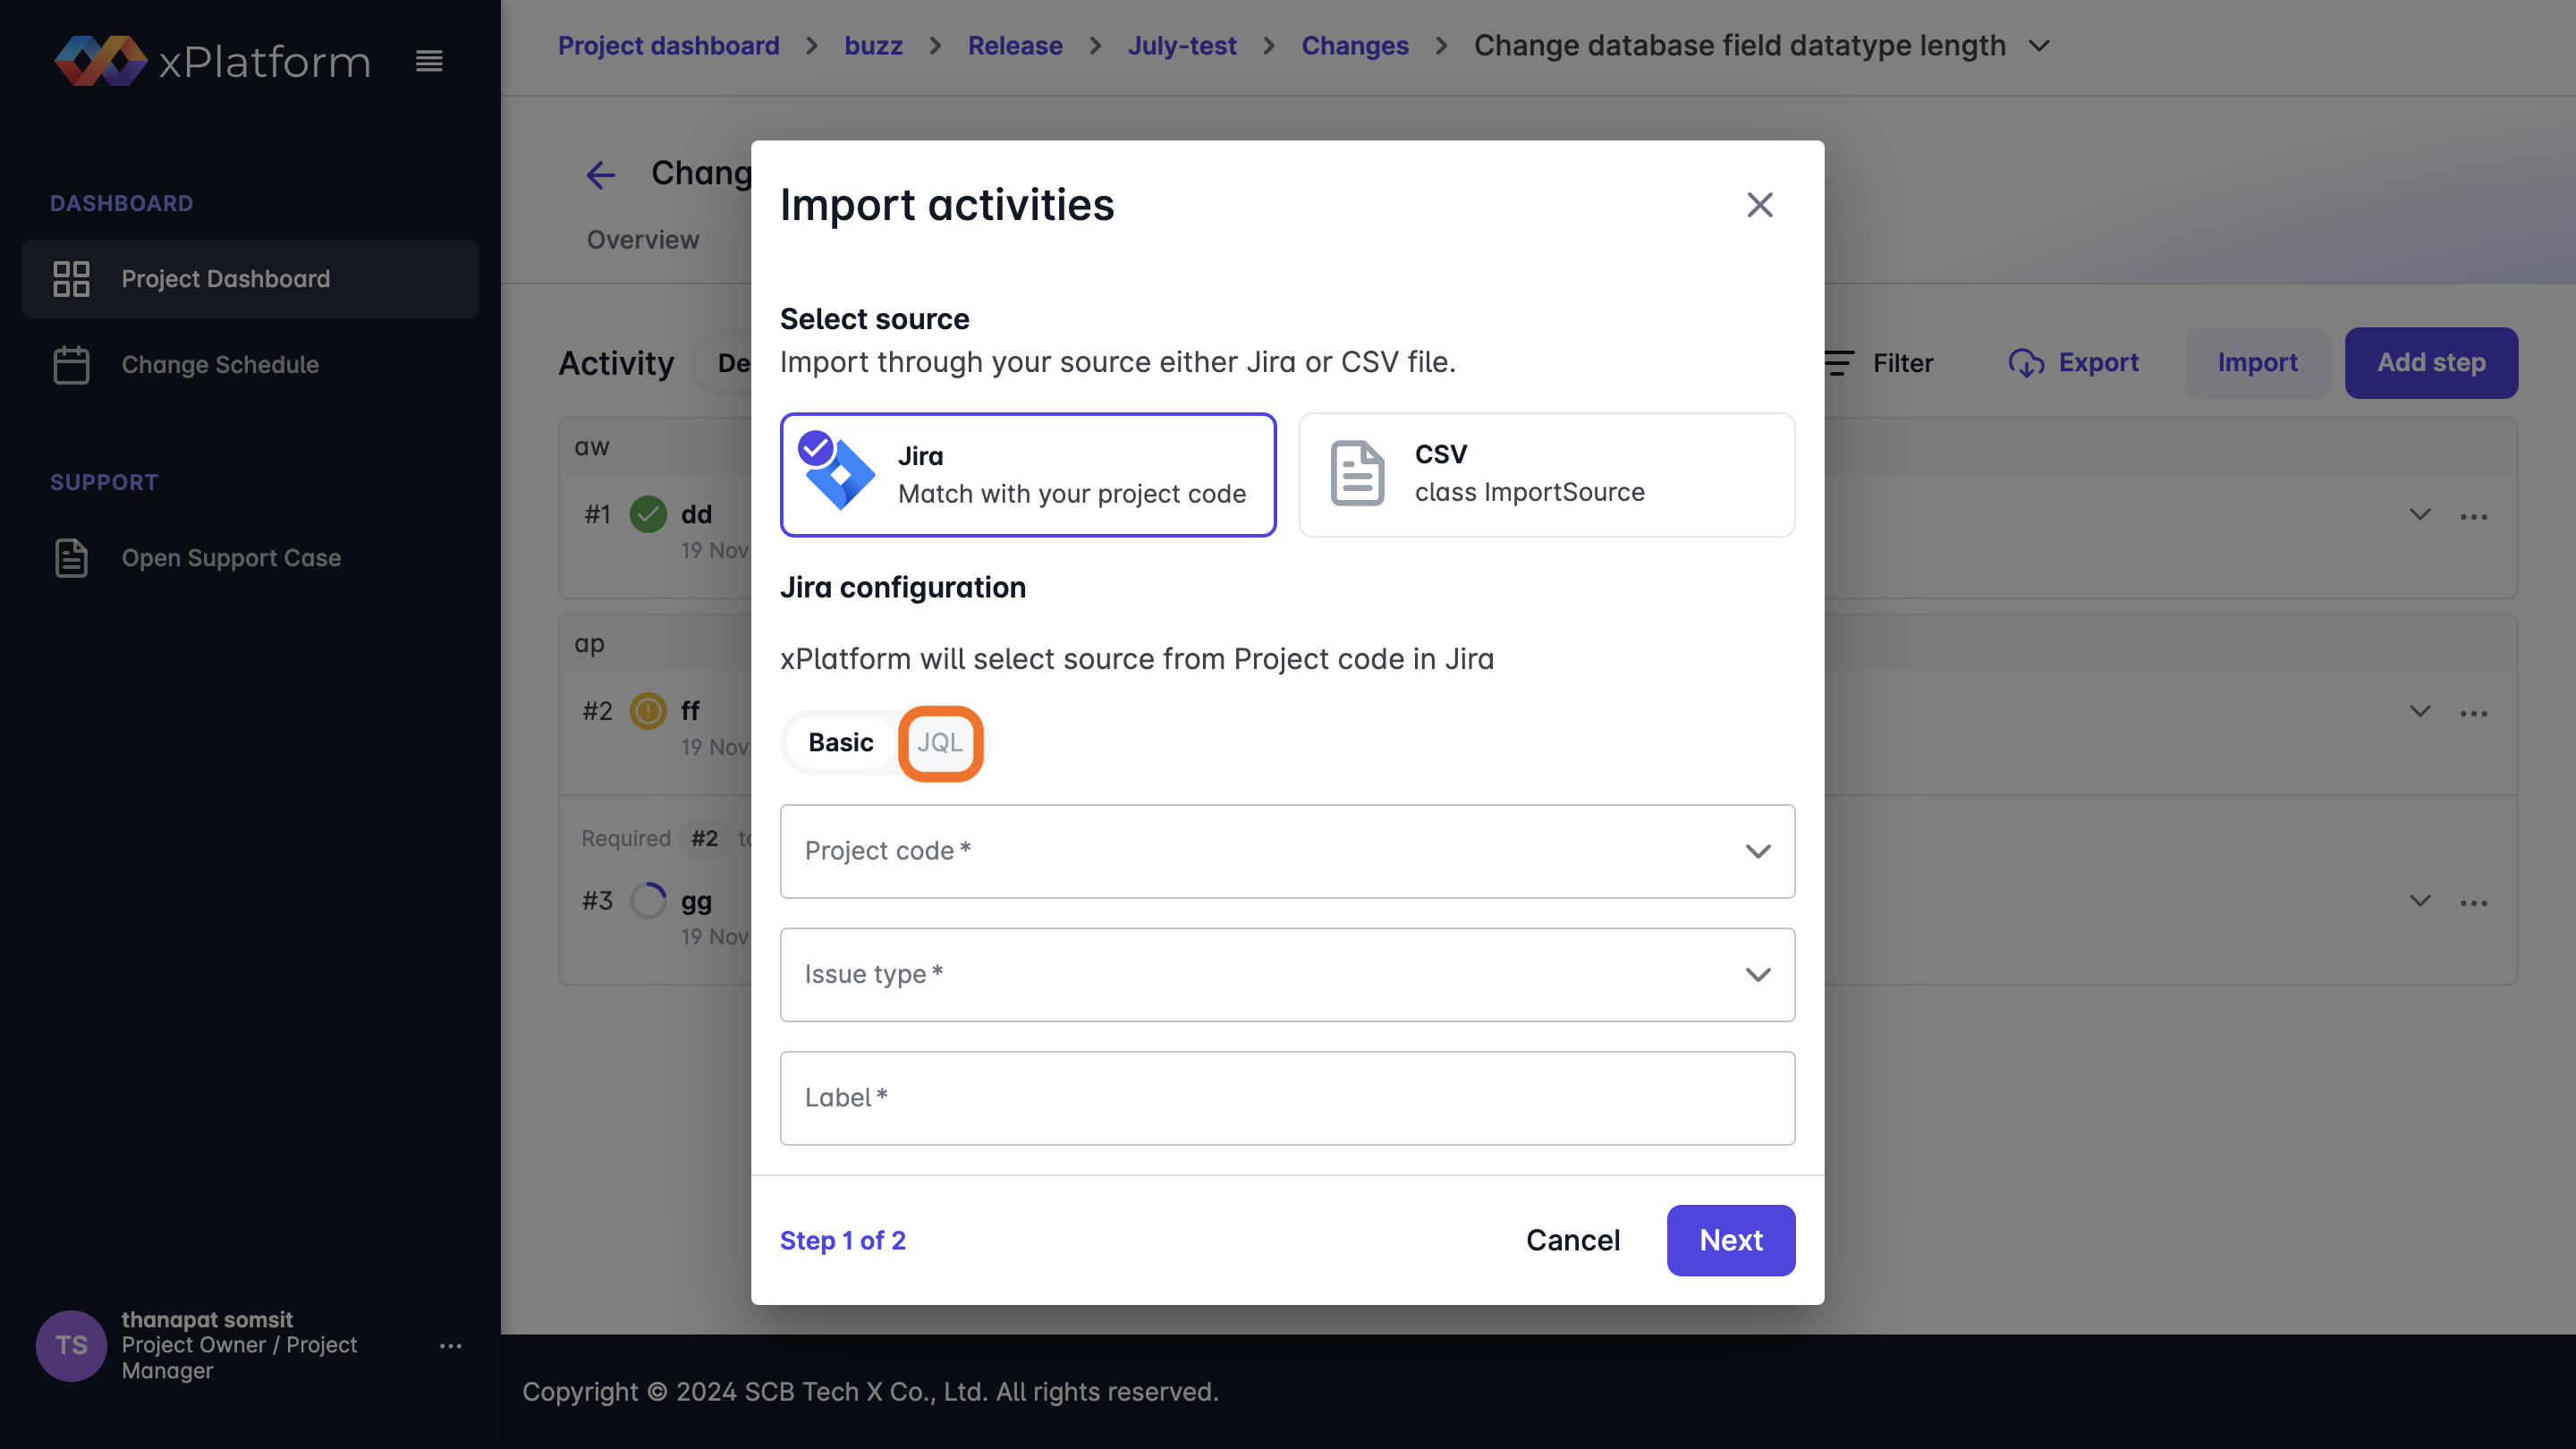
\includegraphics[width=\linewidth]{resources/pages/change-runbook/import-jira/23.png}
\end{center}
\begin{center}
    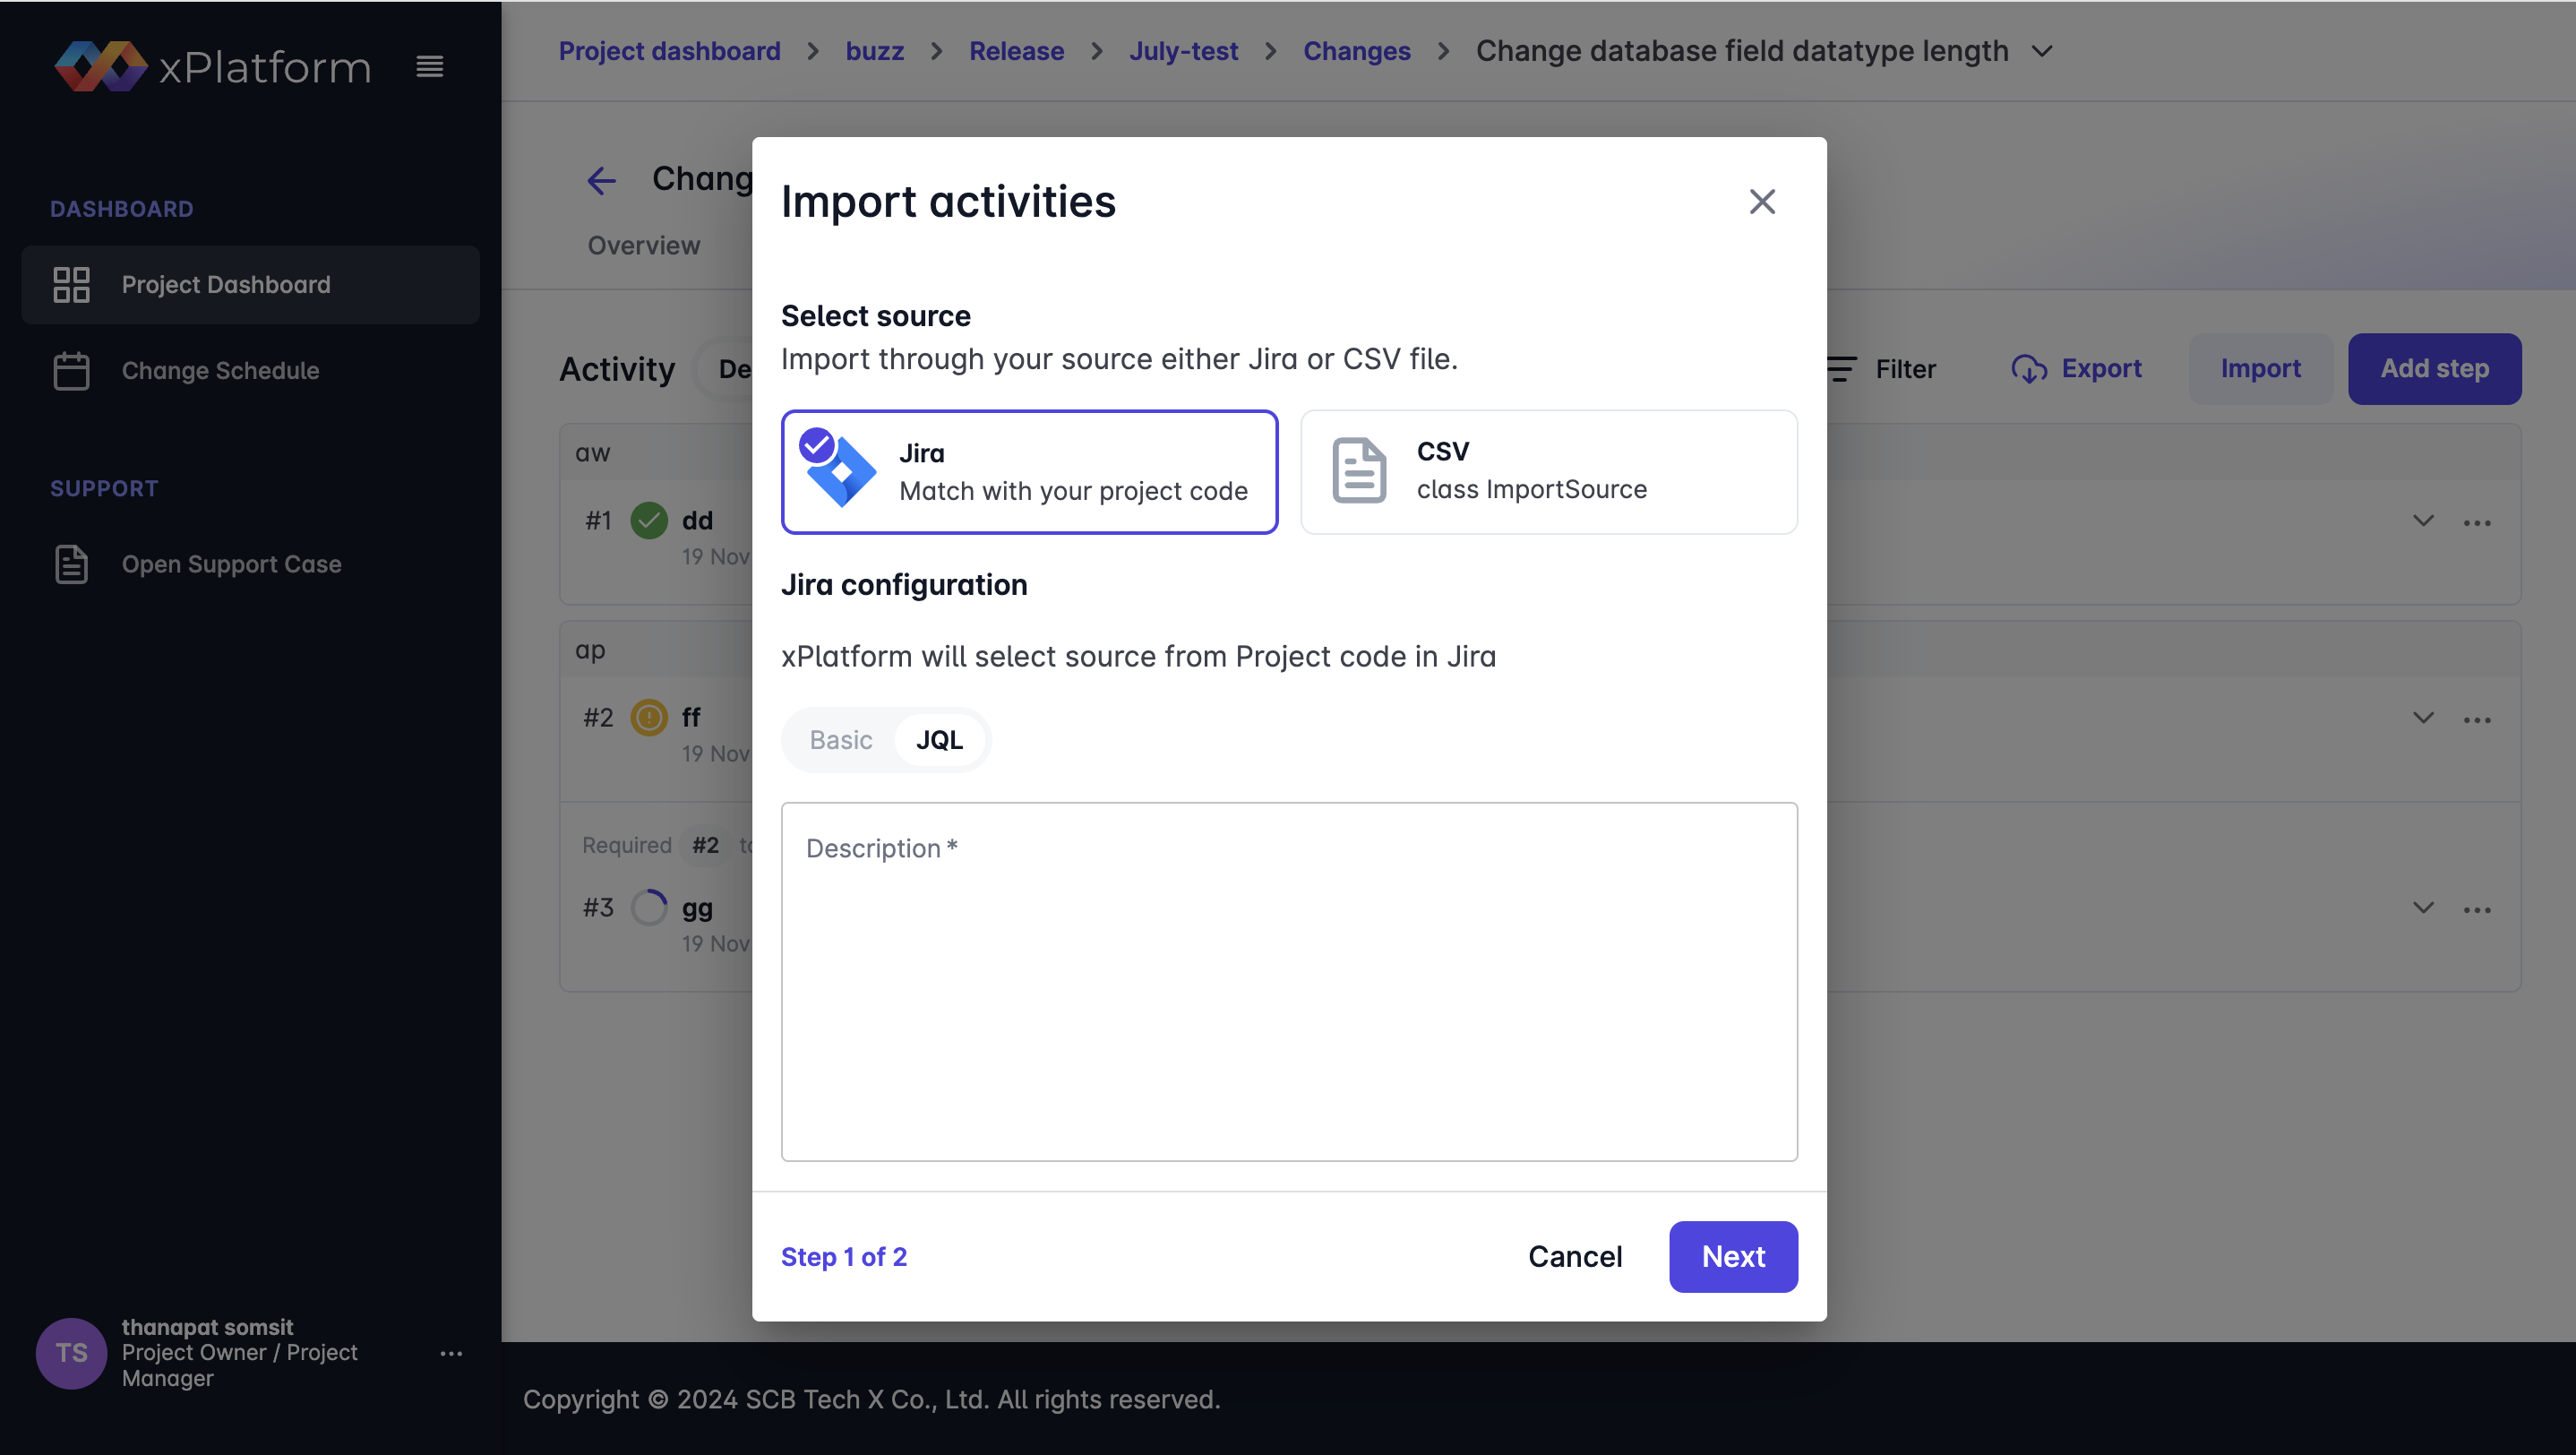
\includegraphics[width=\linewidth]{resources/pages/change-runbook/import-jira/24.png}

    \vspace{1in}

    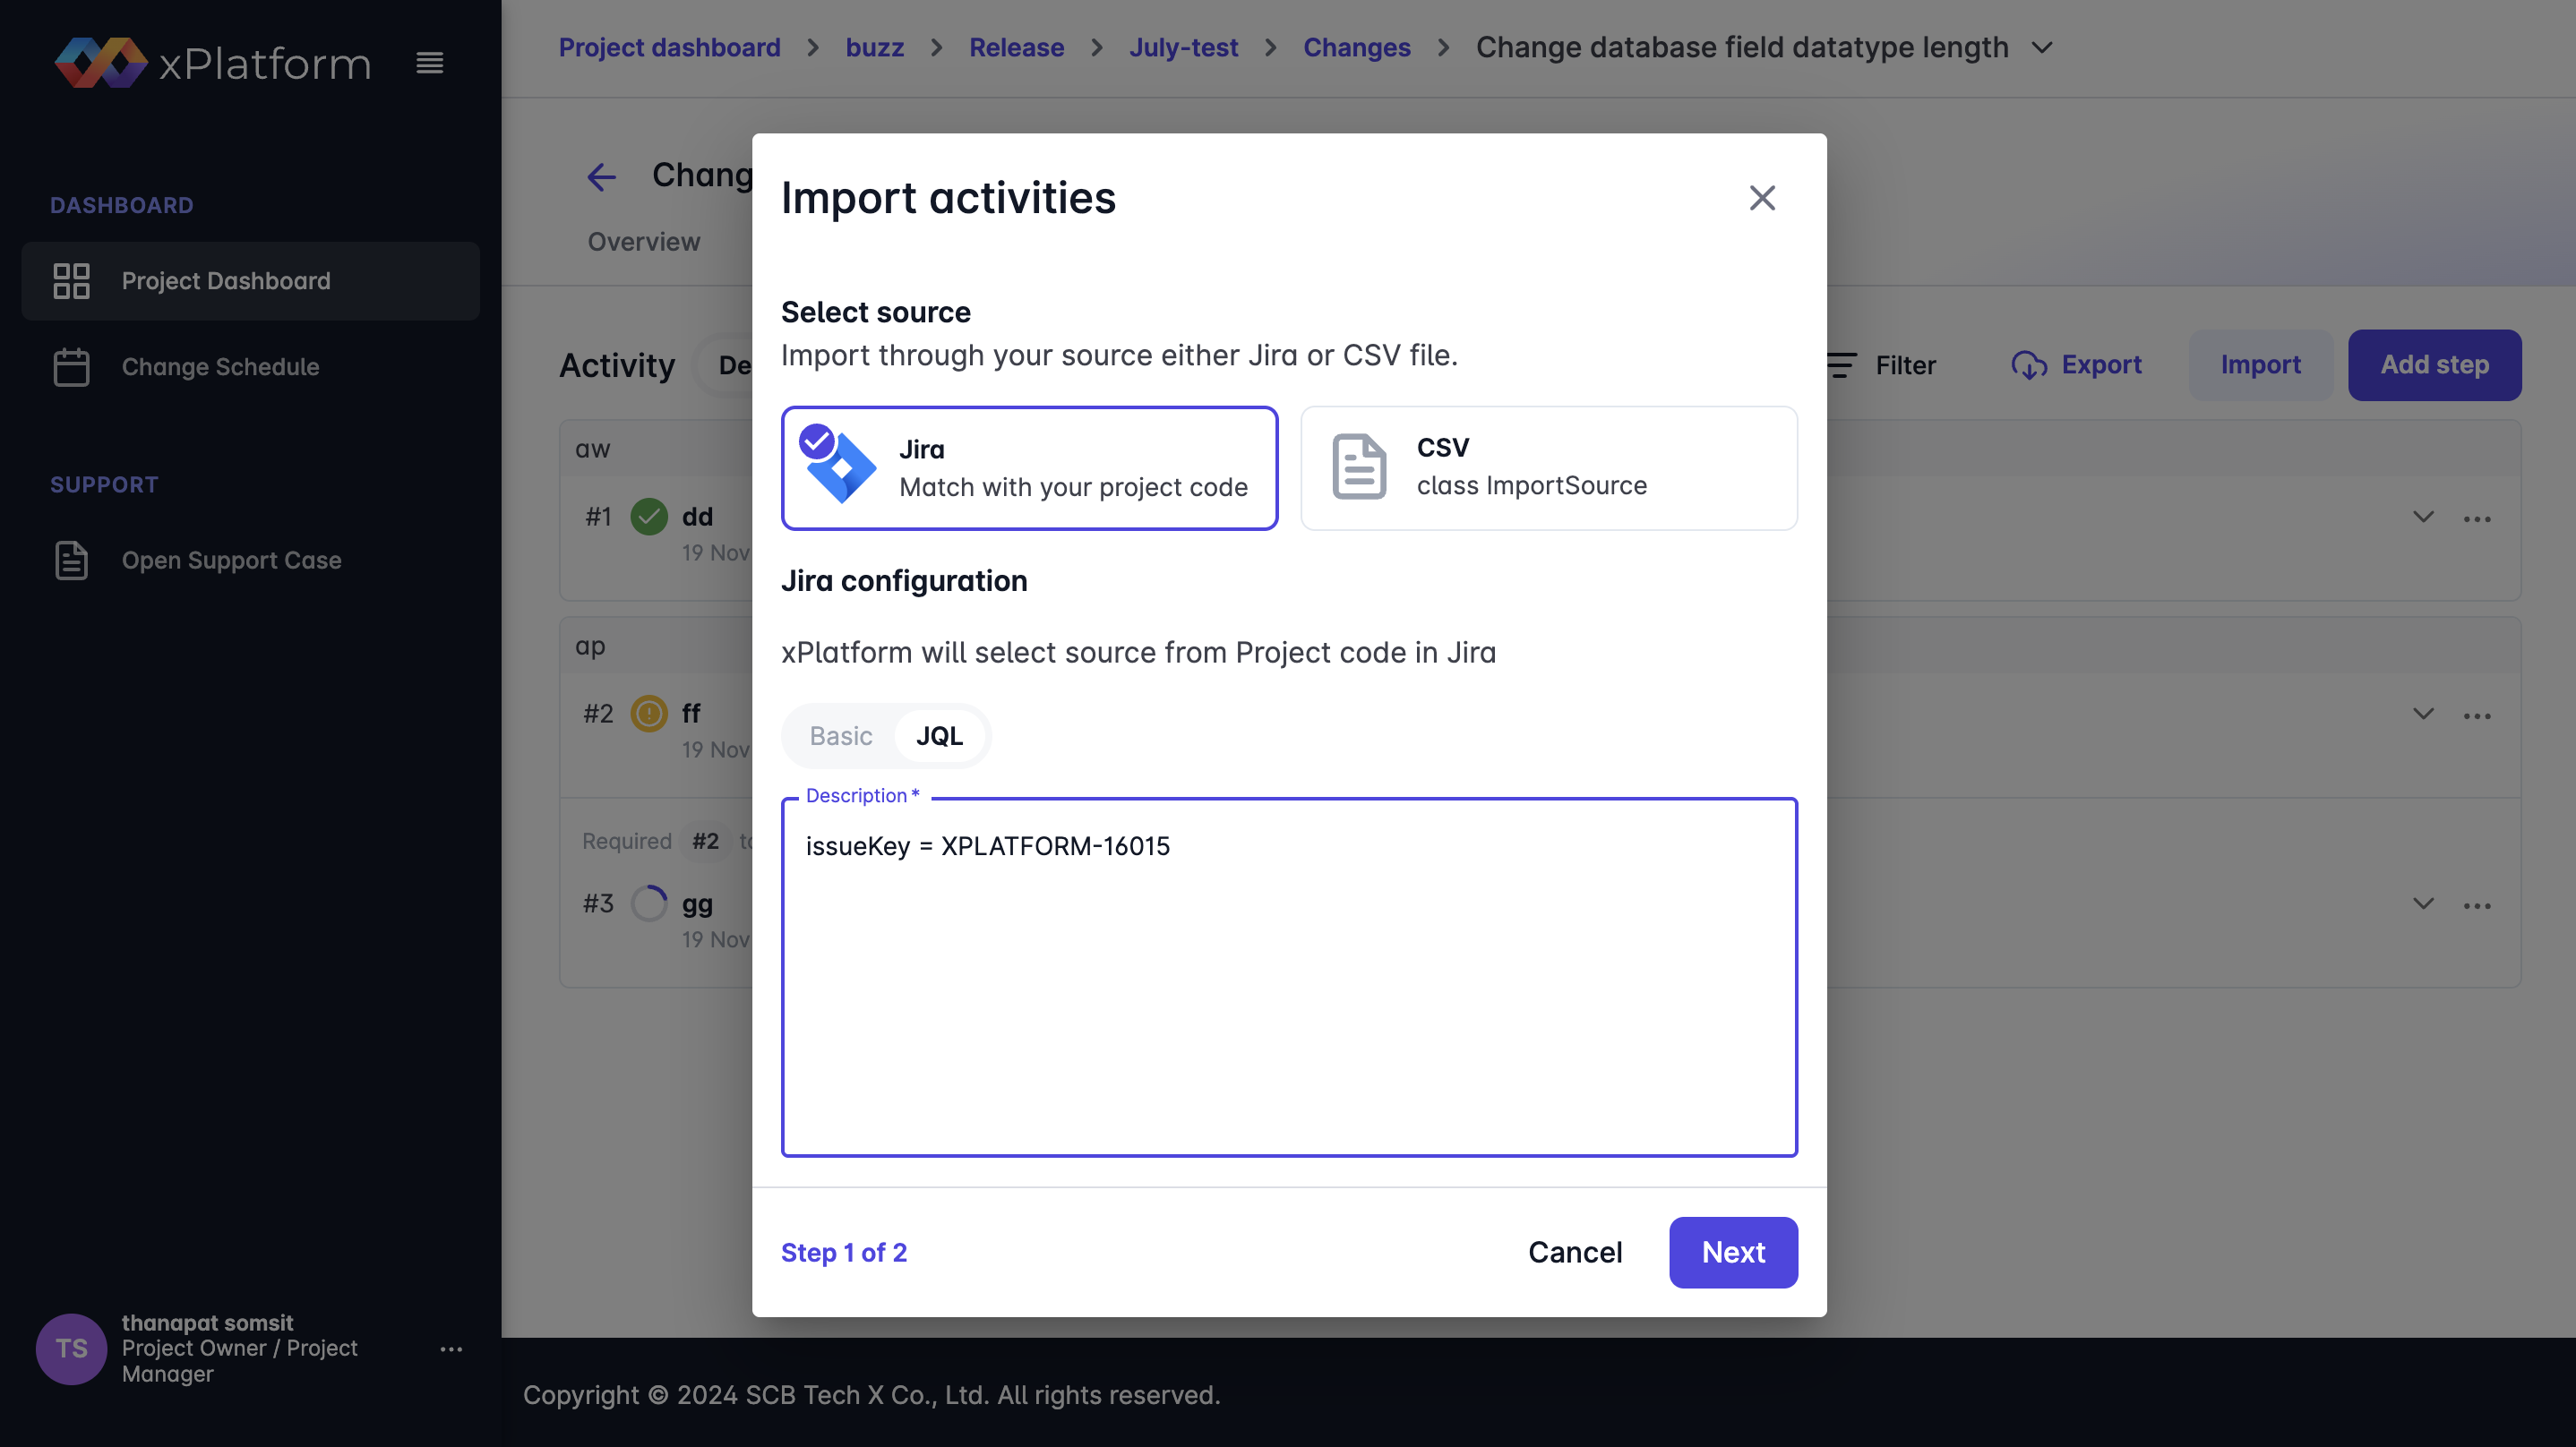
\includegraphics[width=\linewidth]{resources/pages/change-runbook/import-jira/25.png}
\end{center}
\begin{center}
    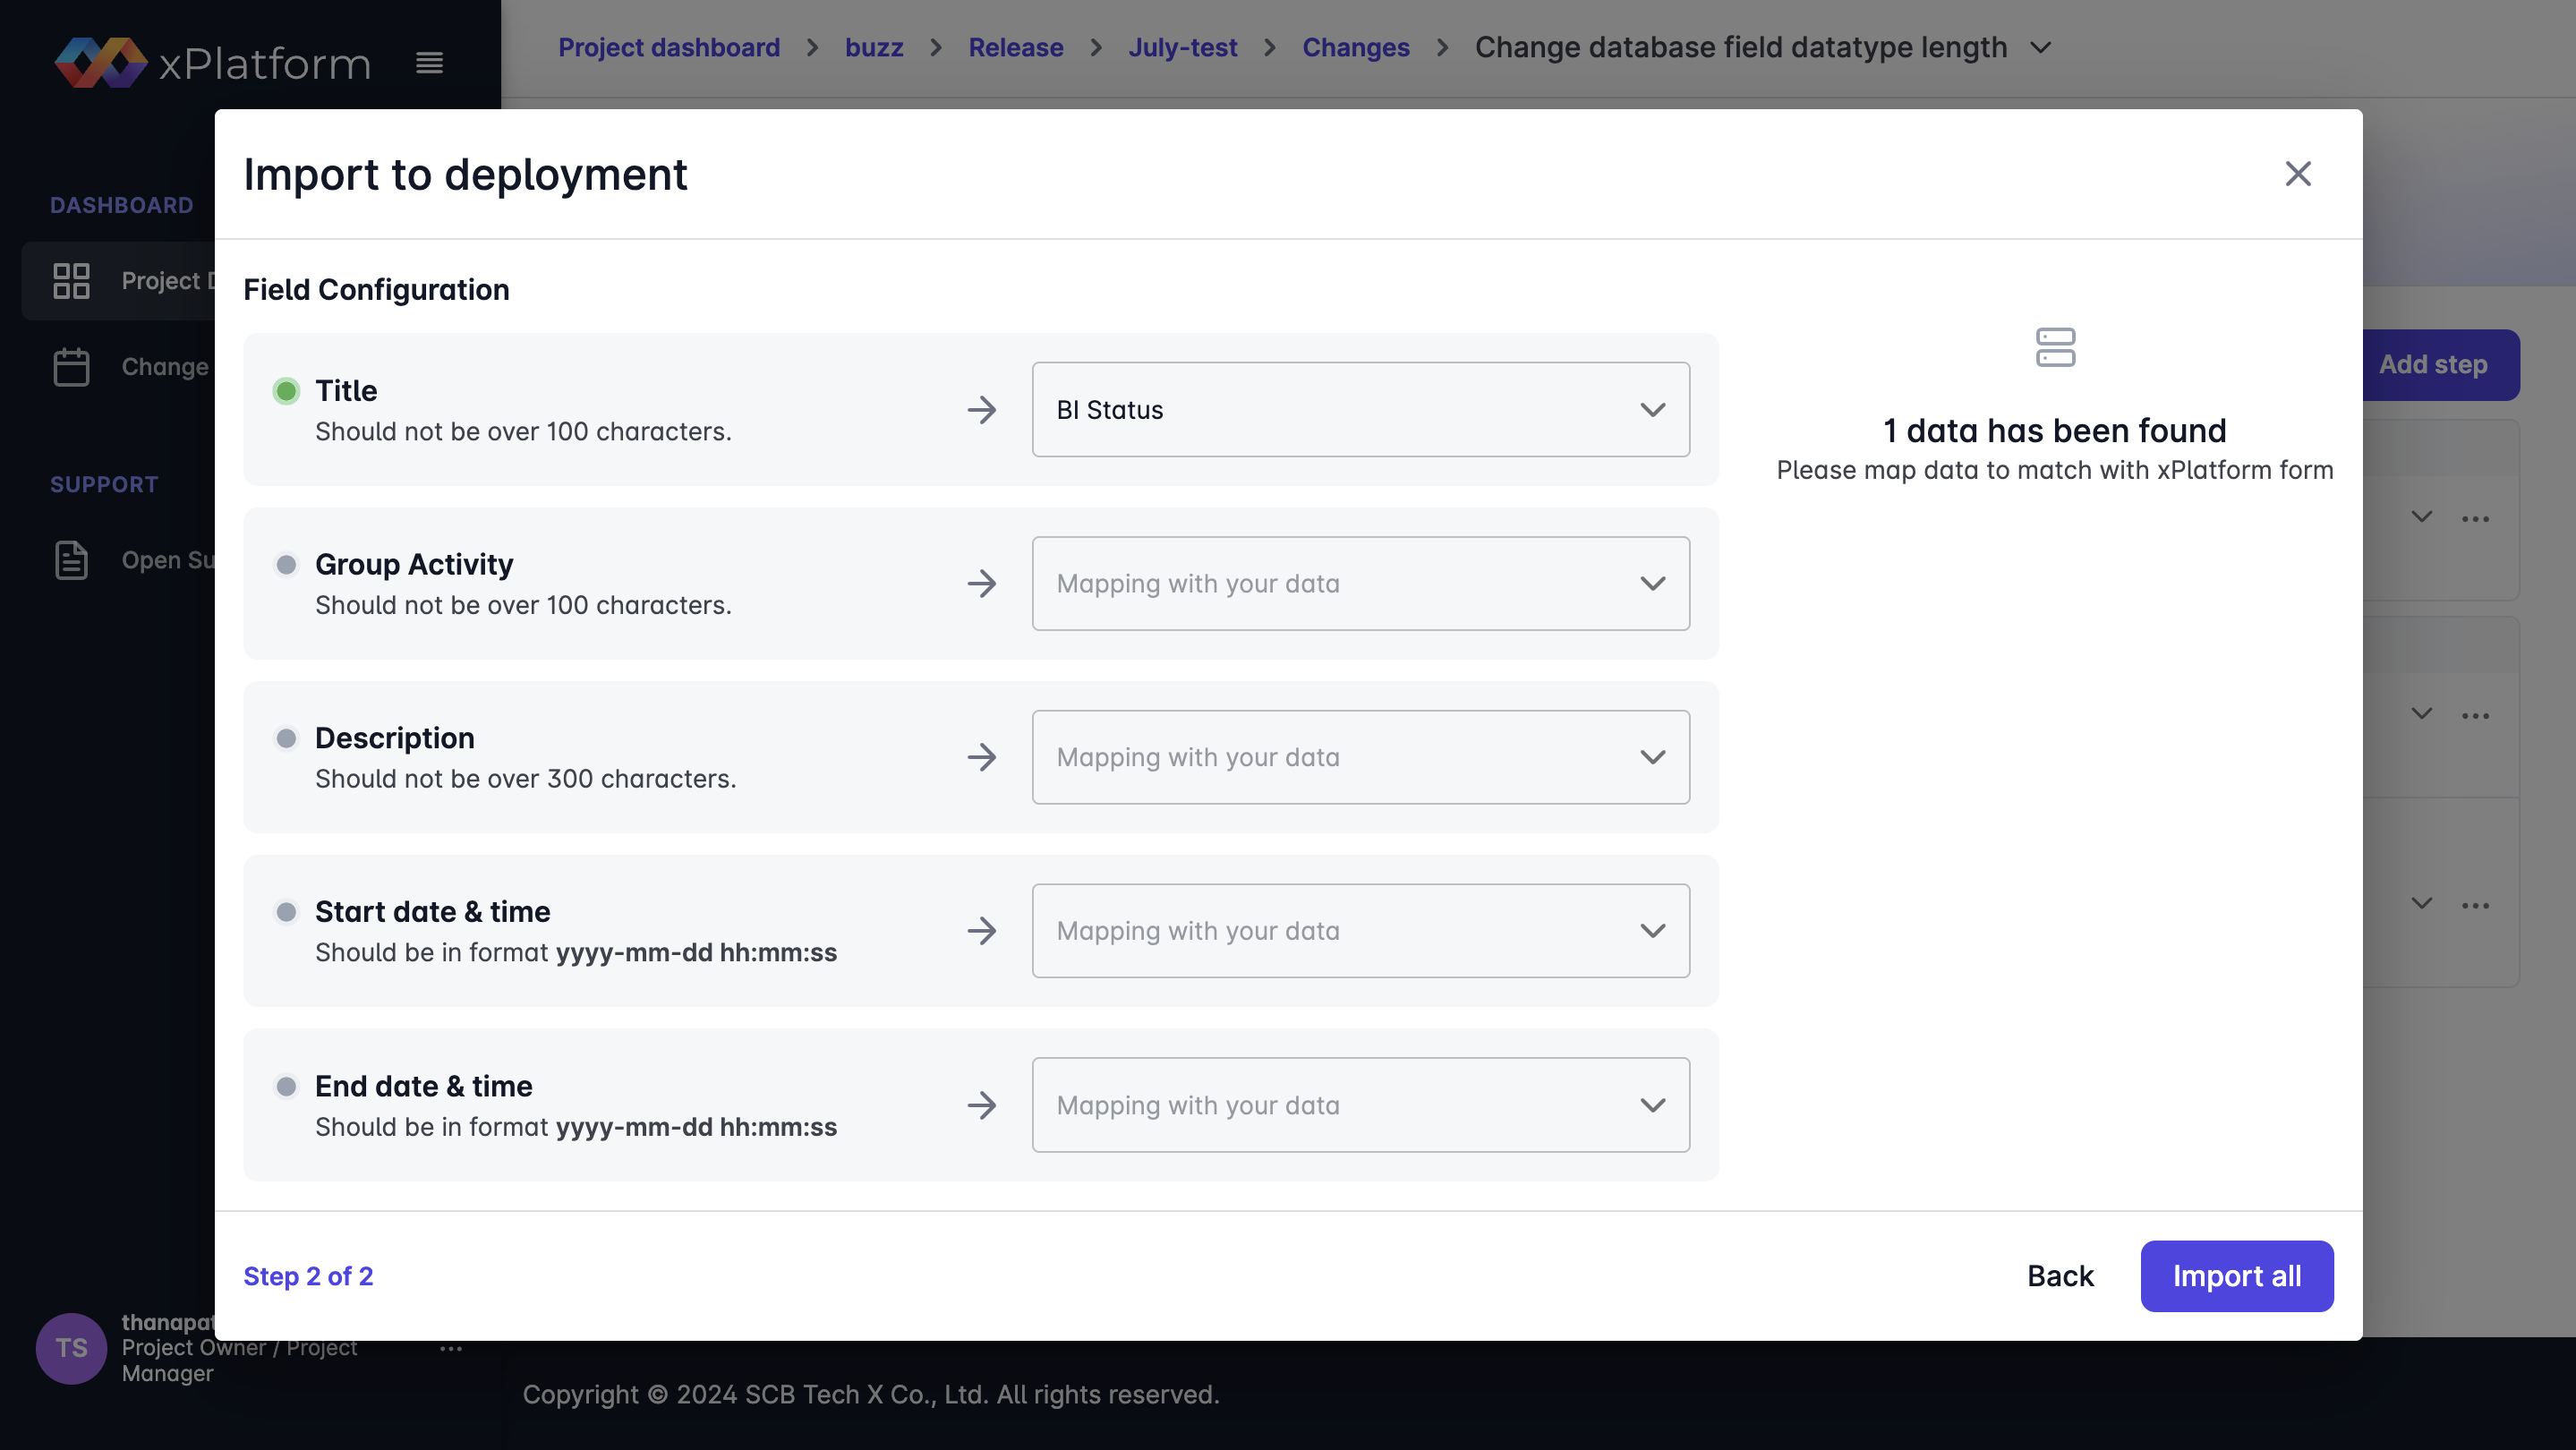
\includegraphics[width=\linewidth]{resources/pages/change-runbook/import-jira/26.png}

    \vspace{1in}

    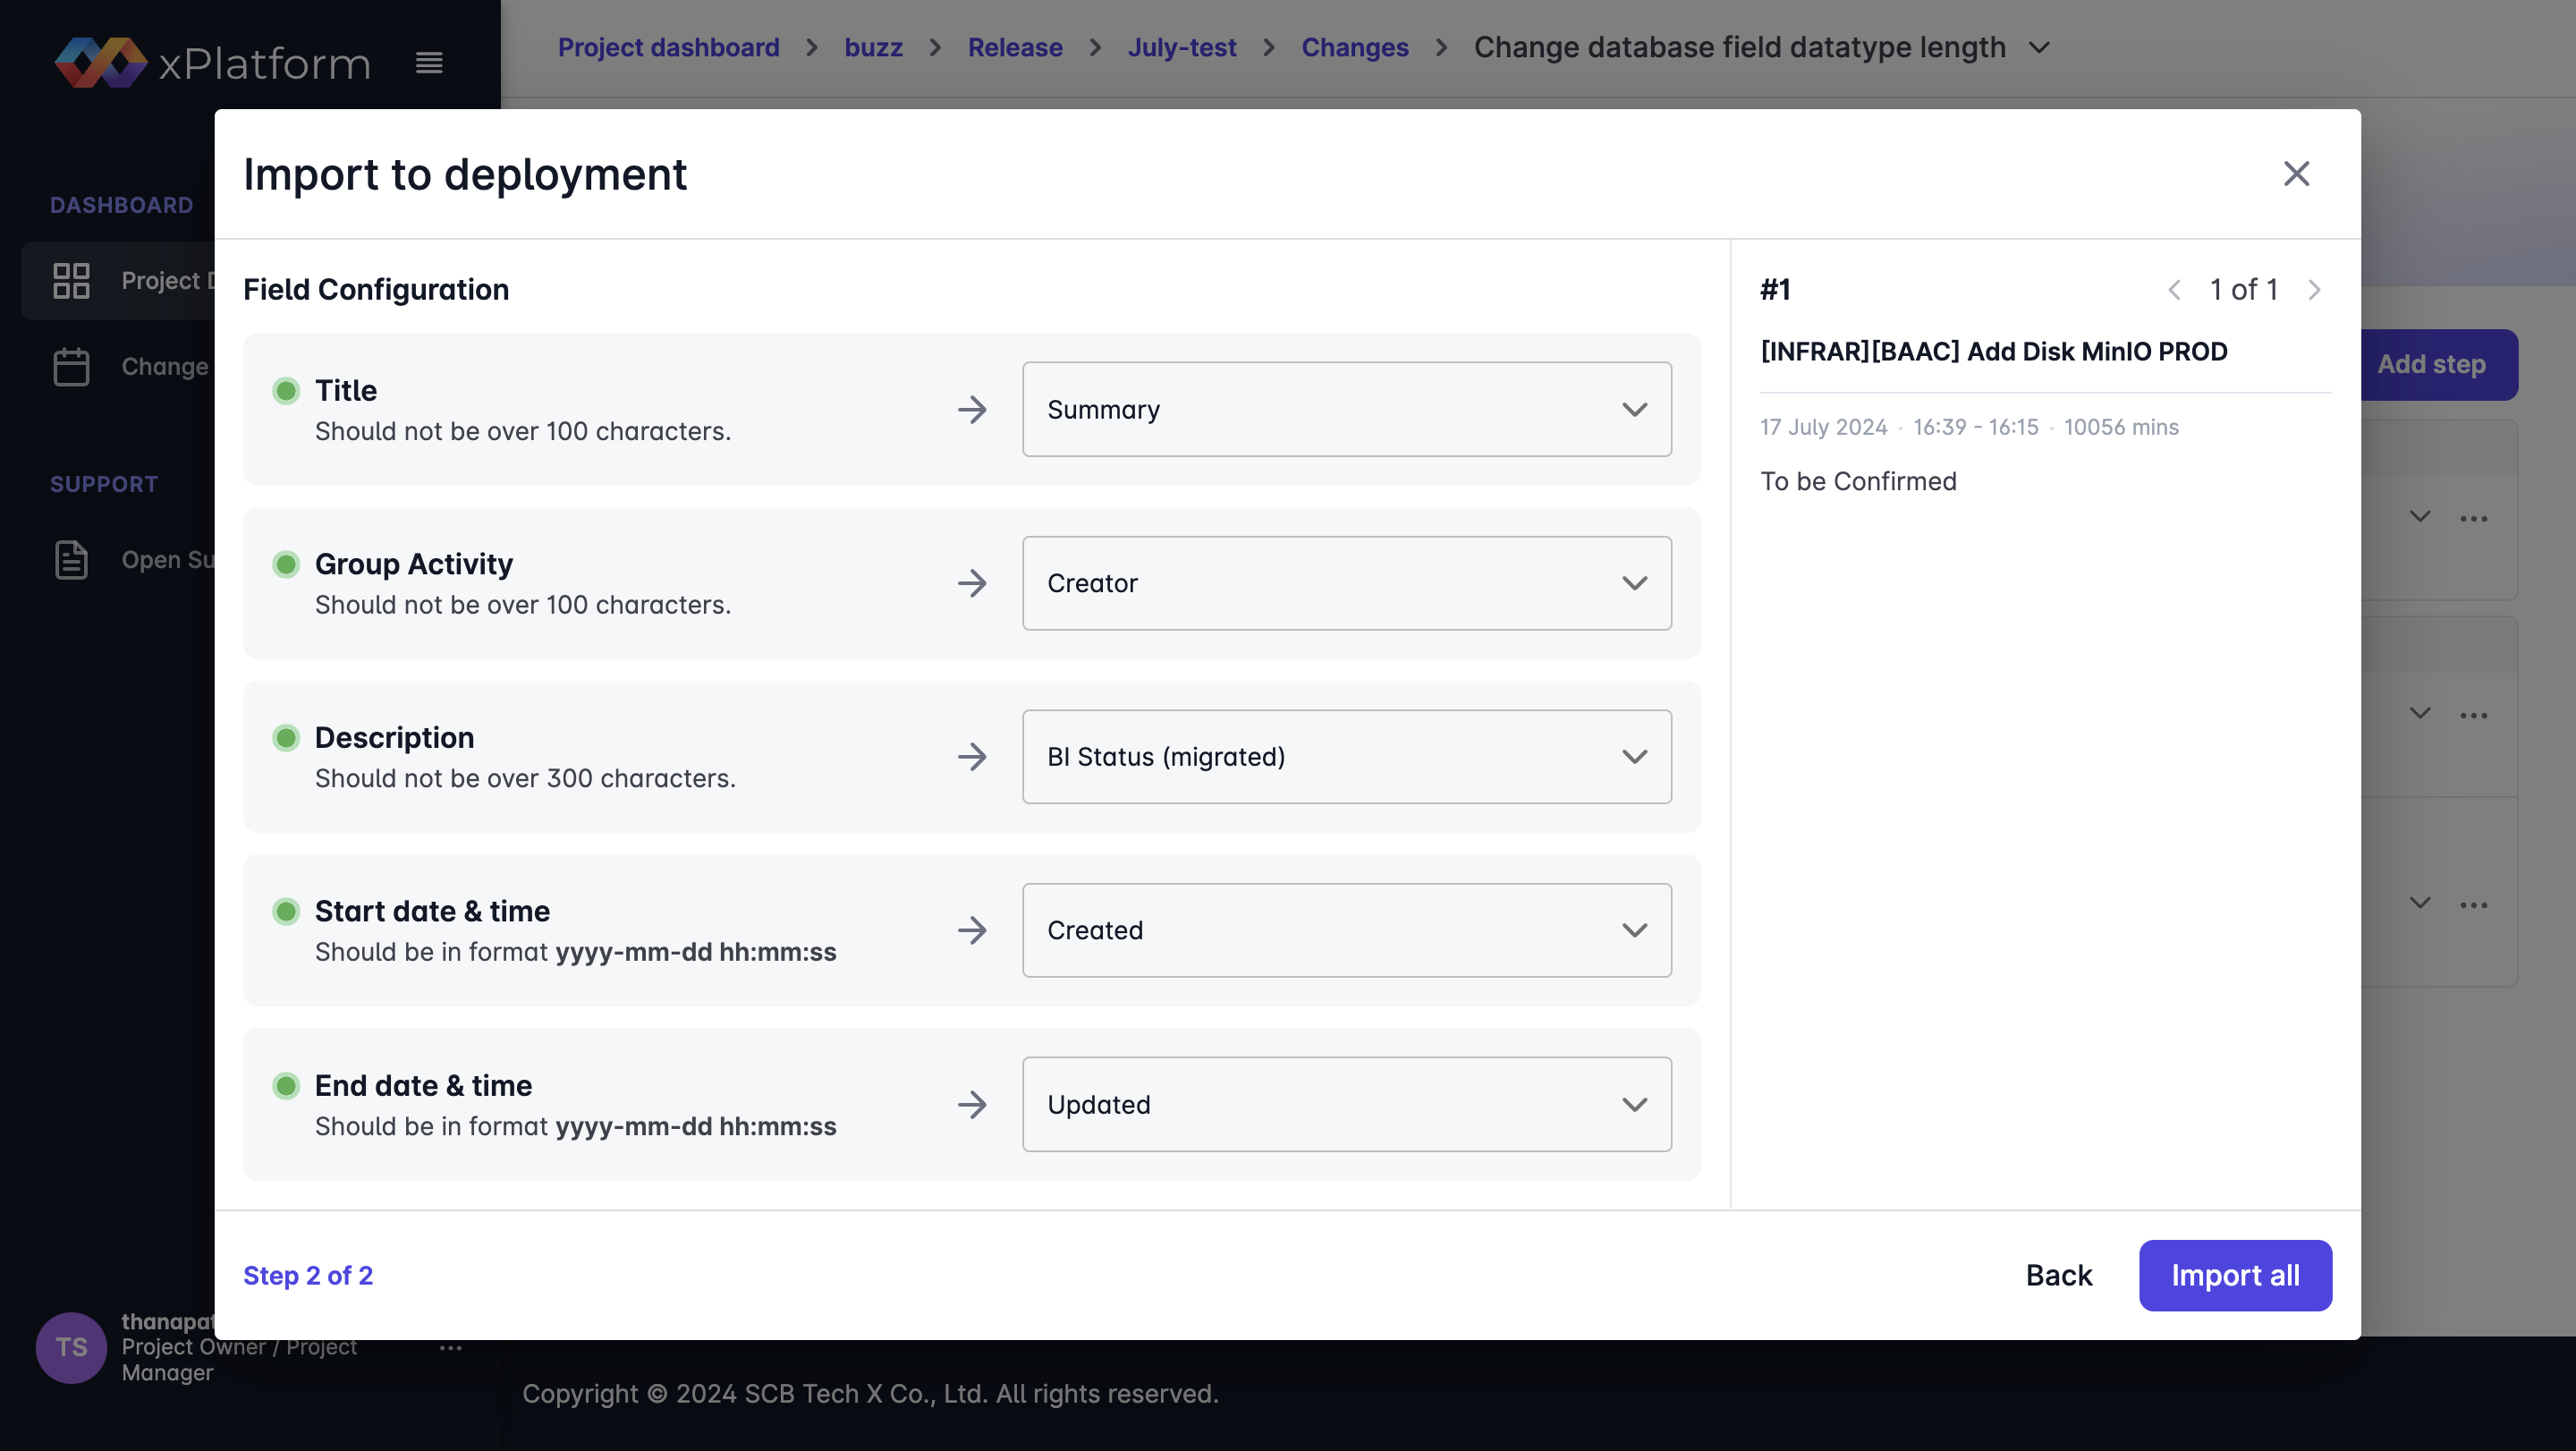
\includegraphics[width=\linewidth]{resources/pages/change-runbook/import-jira/27.png}
\end{center}

\begin{figure}[H]
    \begin{center}
        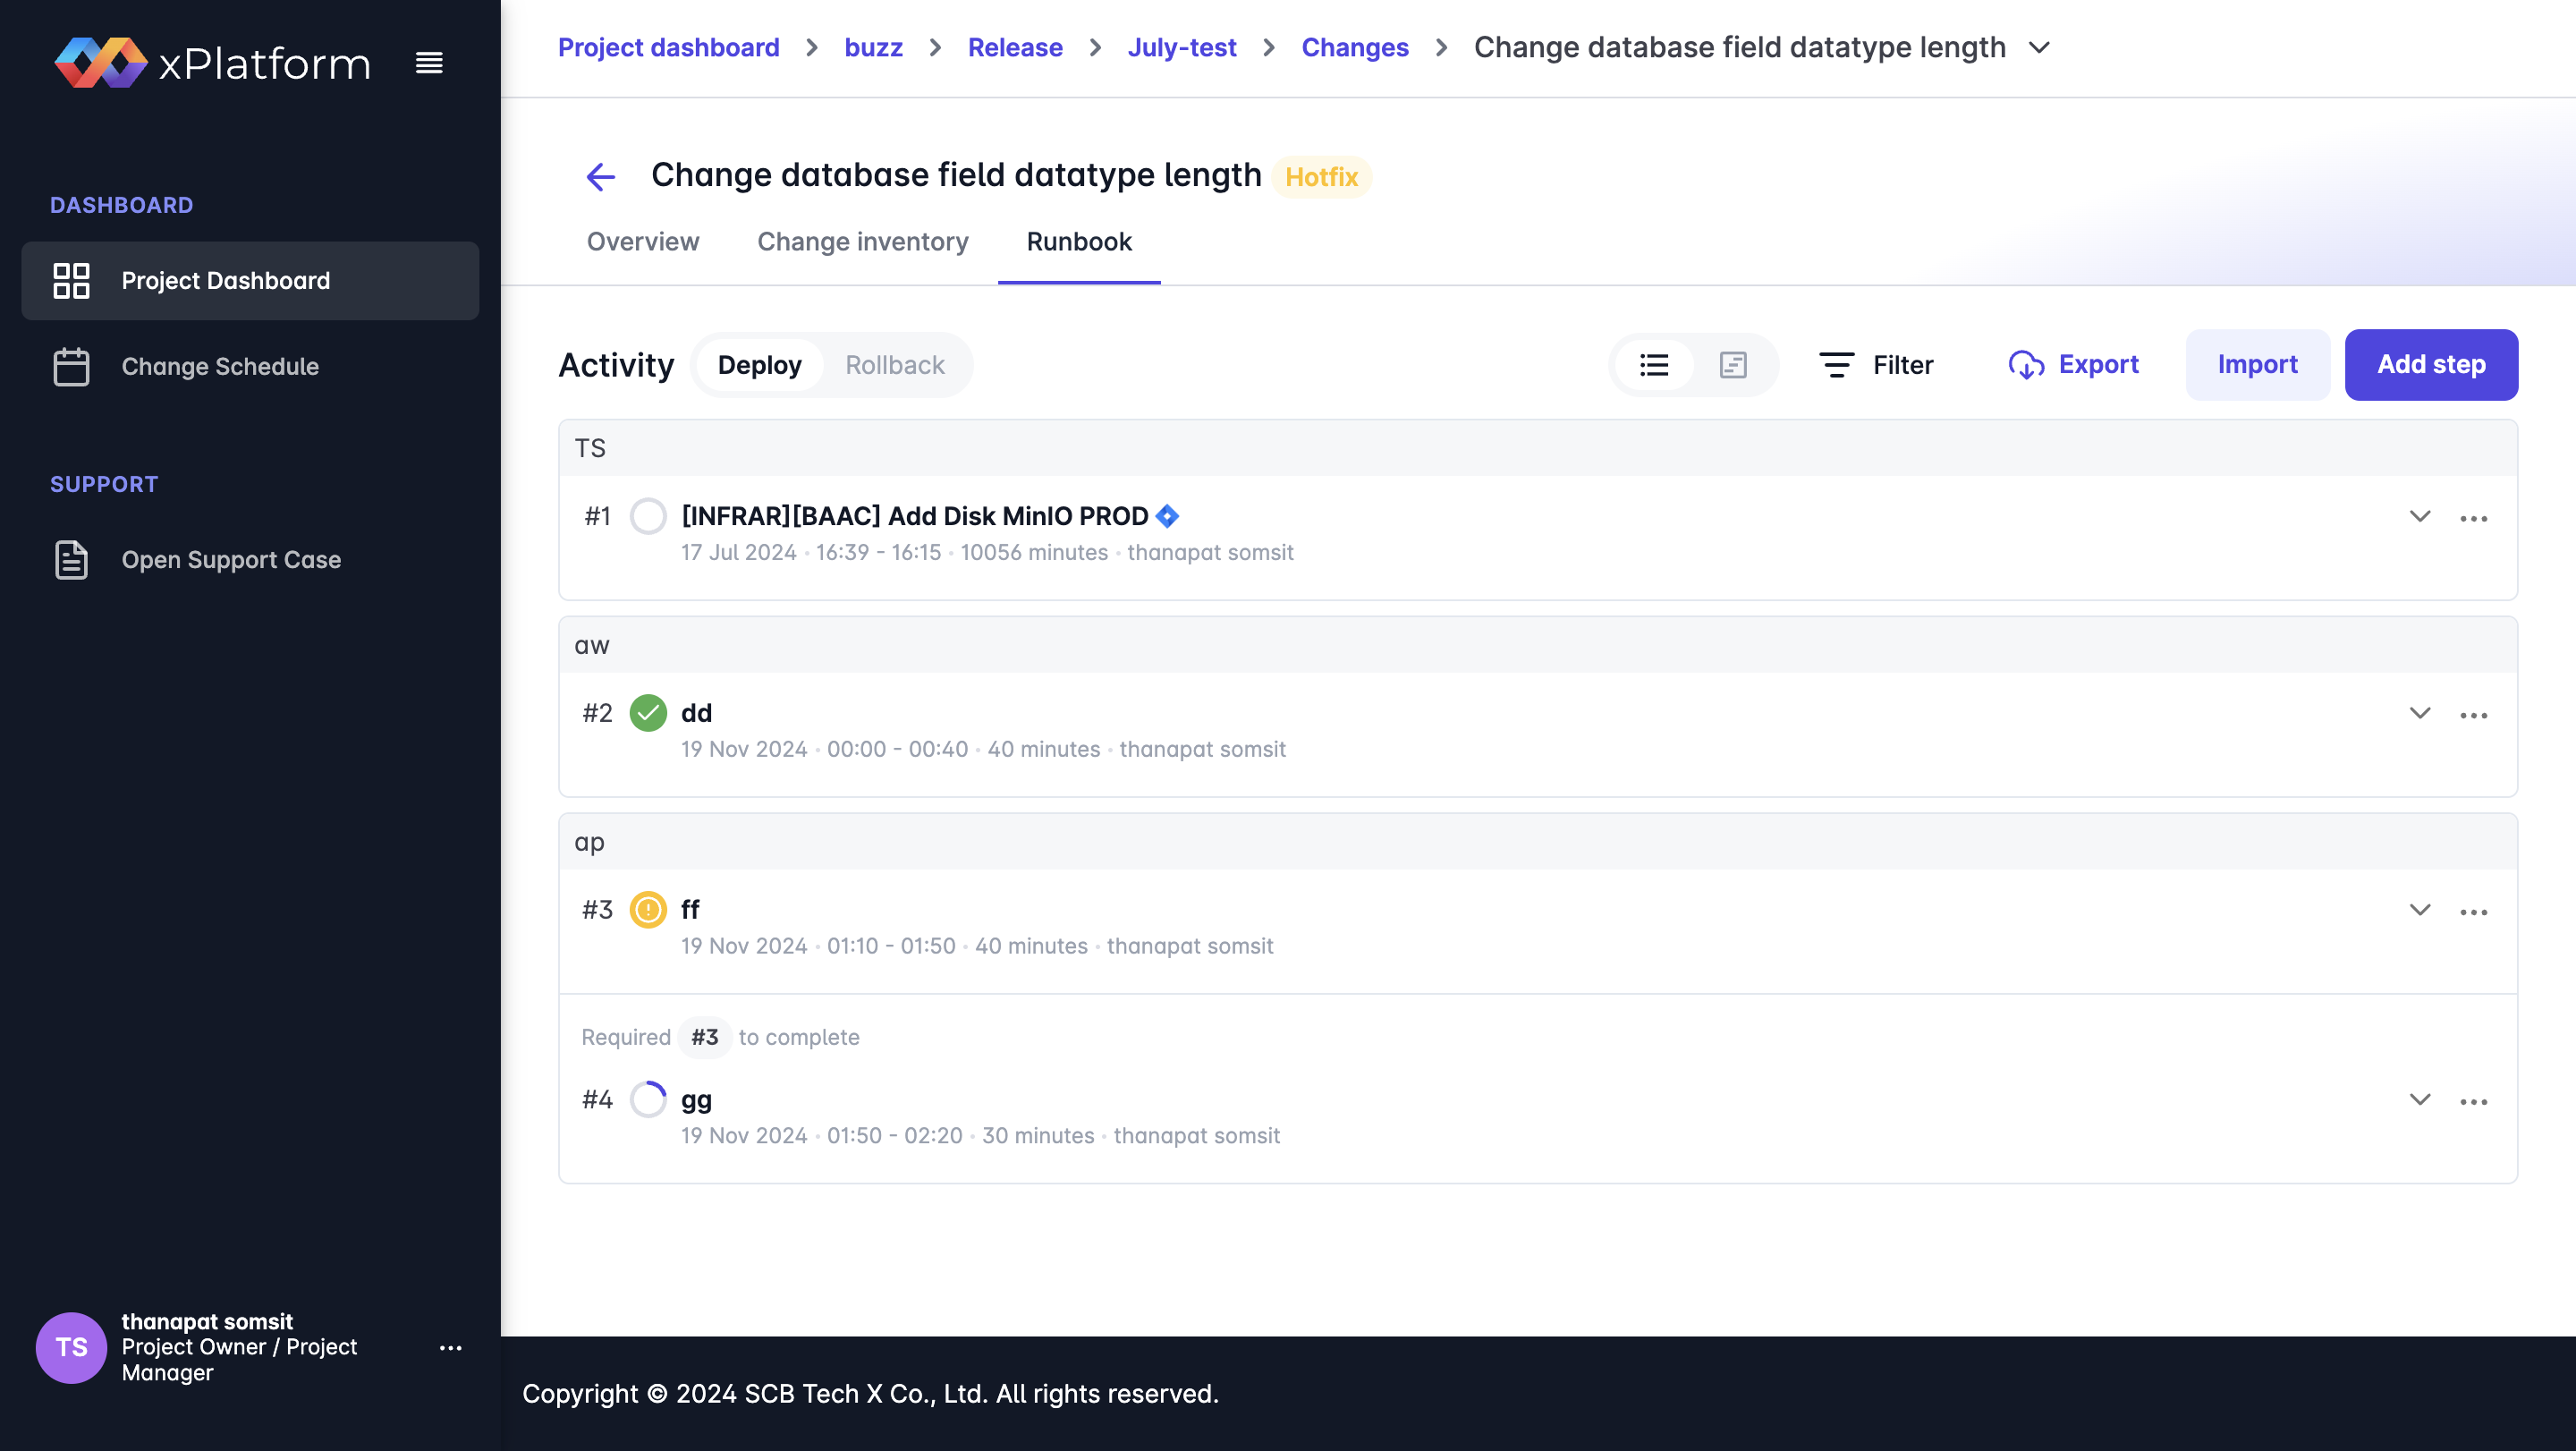
\includegraphics[width=\linewidth]{resources/pages/change-runbook/import-jira/28.png}
    \end{center}
    \caption[การดึงข้อมูลจาก Jira]{การดึงข้อมูลจาก Jira}
  \label{fig:import-jira}
\end{figure}

\newpage
\subsection{การดึงข้อมูลจาก CSV}
\begin{center}
    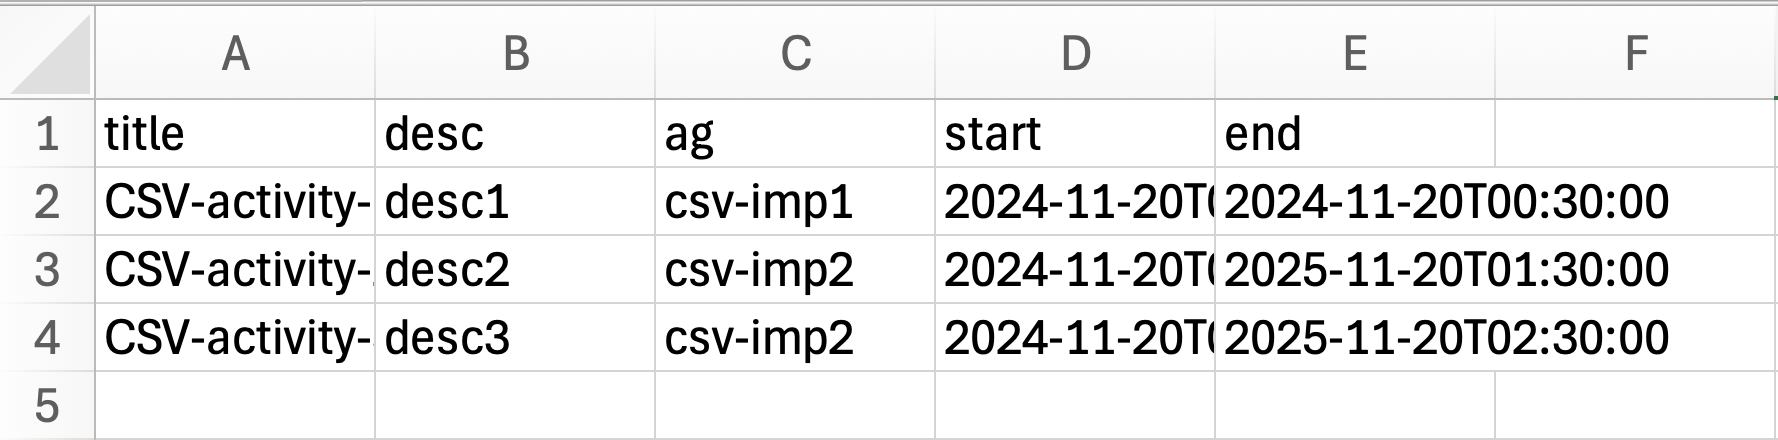
\includegraphics[width=\linewidth]{resources/pages/change-runbook/import-csv/29.png}

    \vspace{1in}

    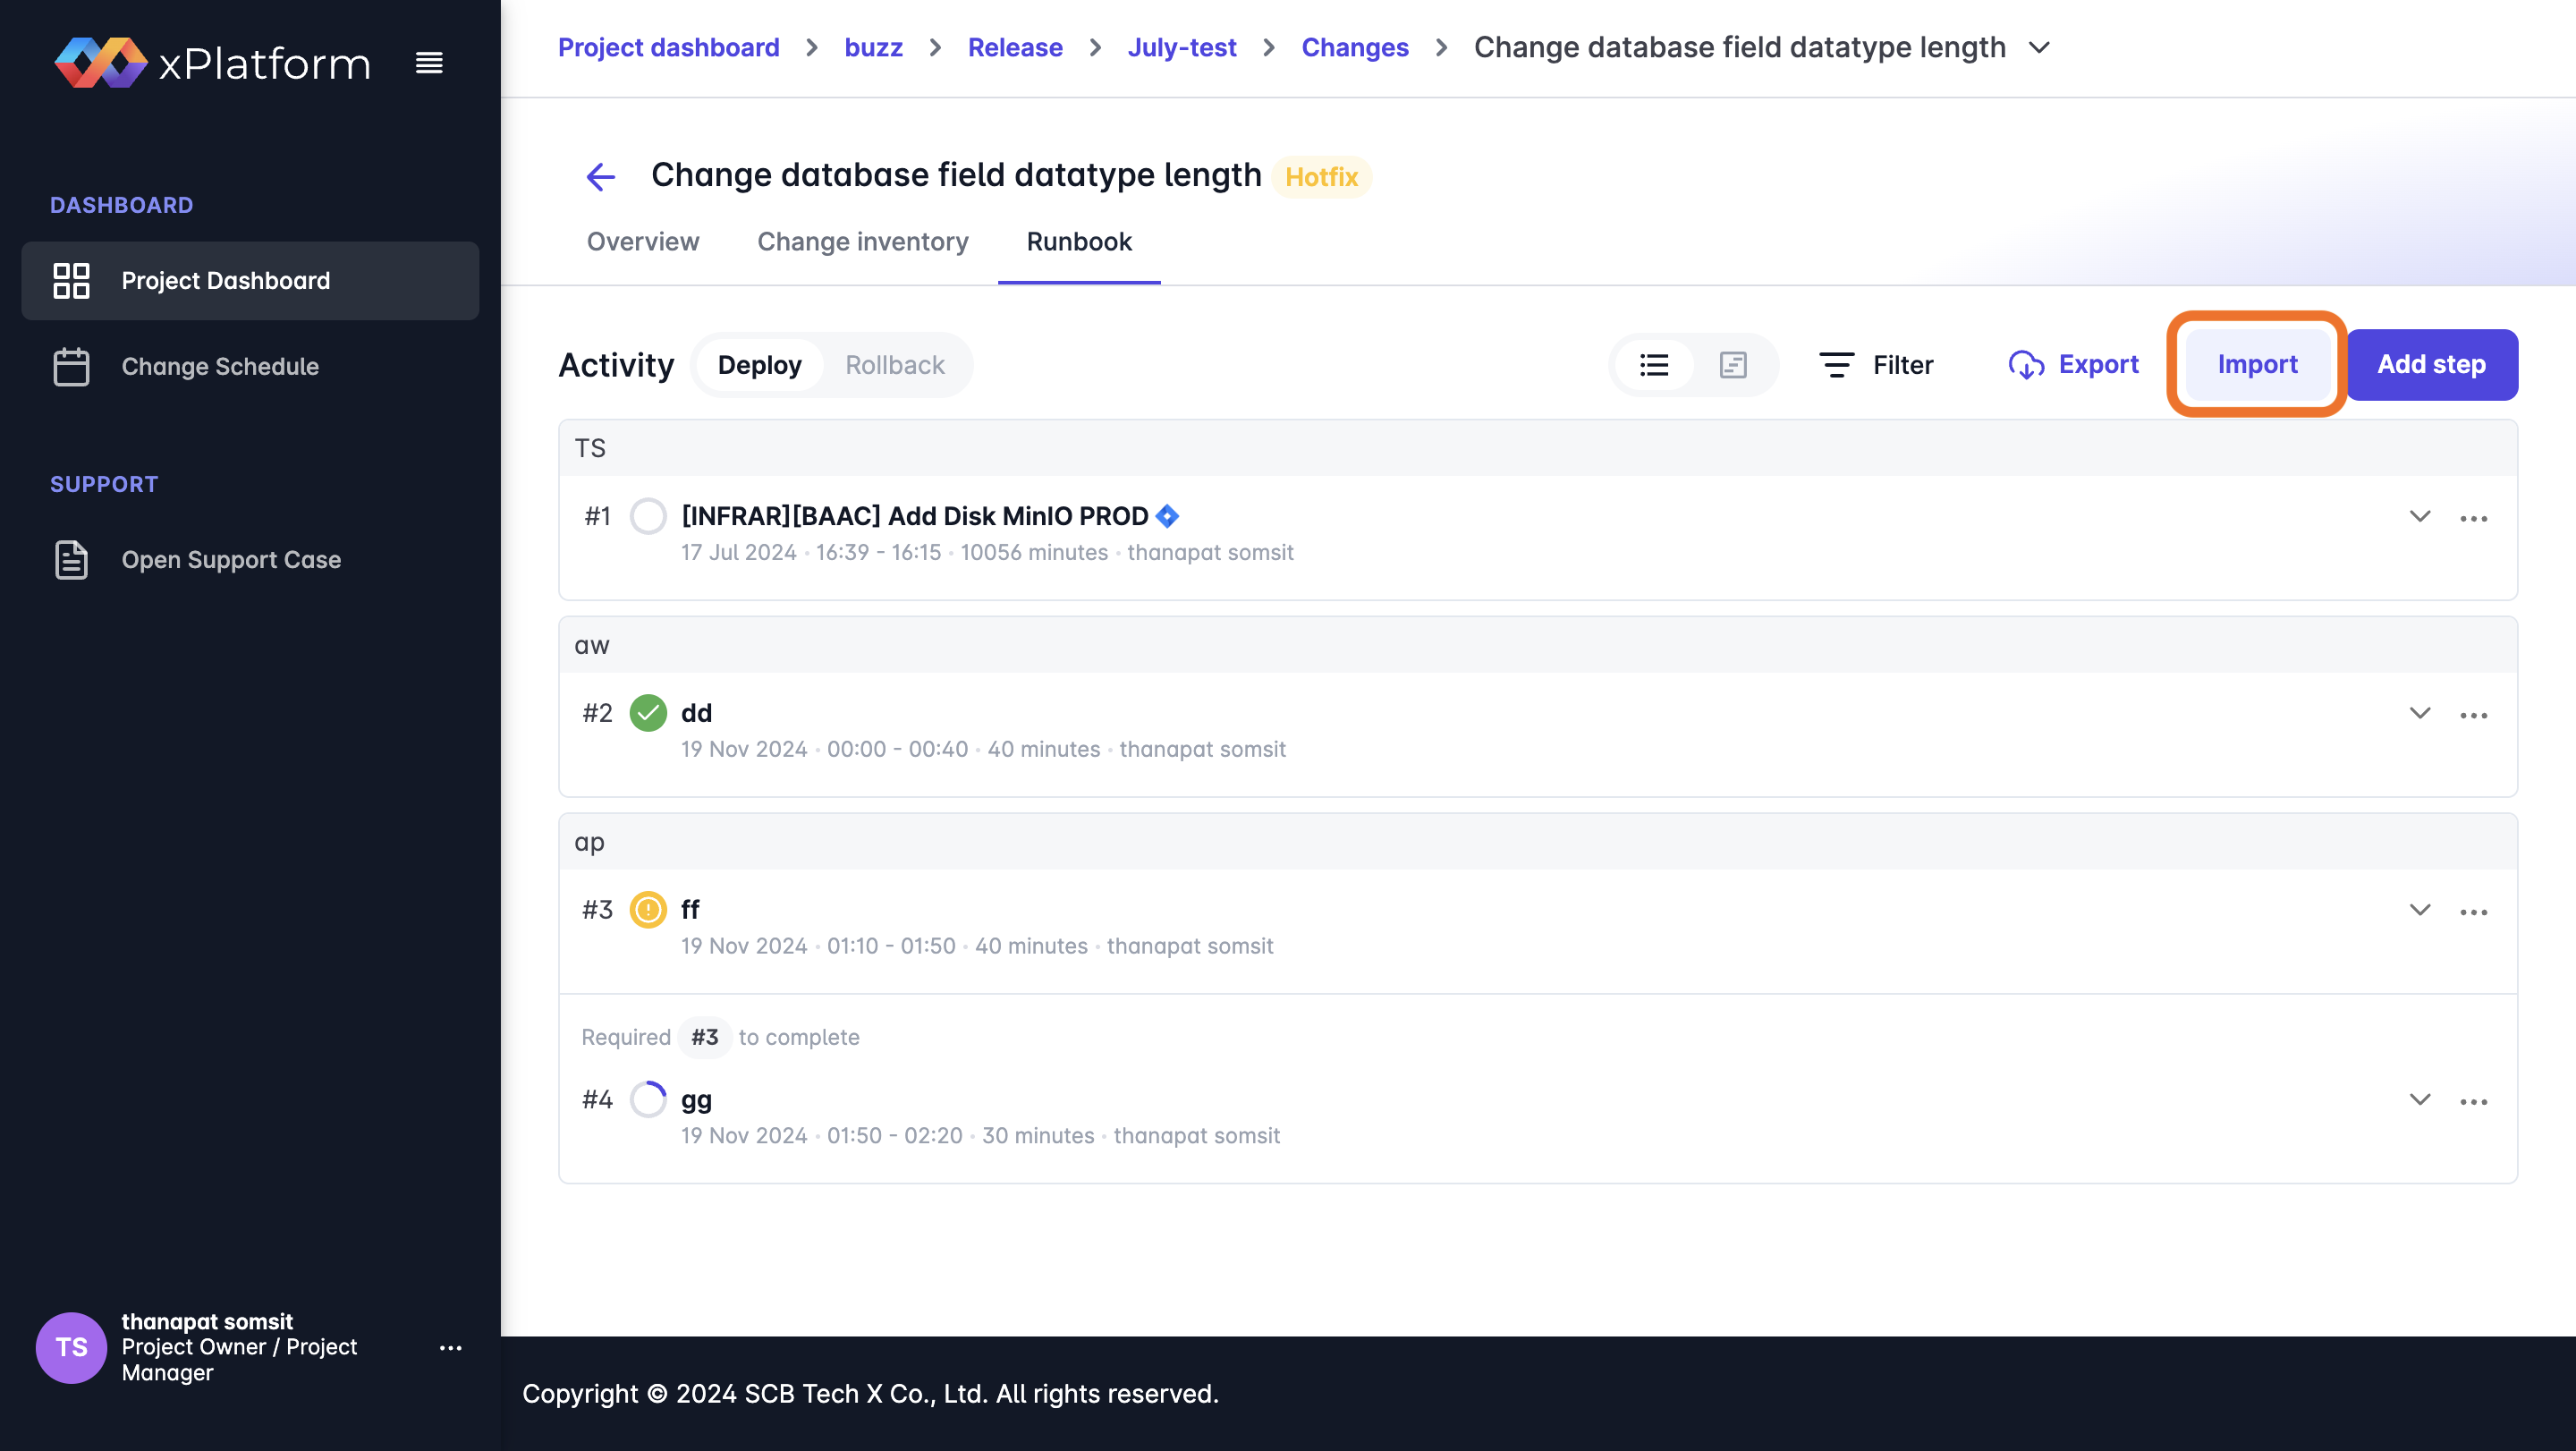
\includegraphics[width=\linewidth]{resources/pages/change-runbook/import-csv/30.png}
\end{center}
\begin{center}
    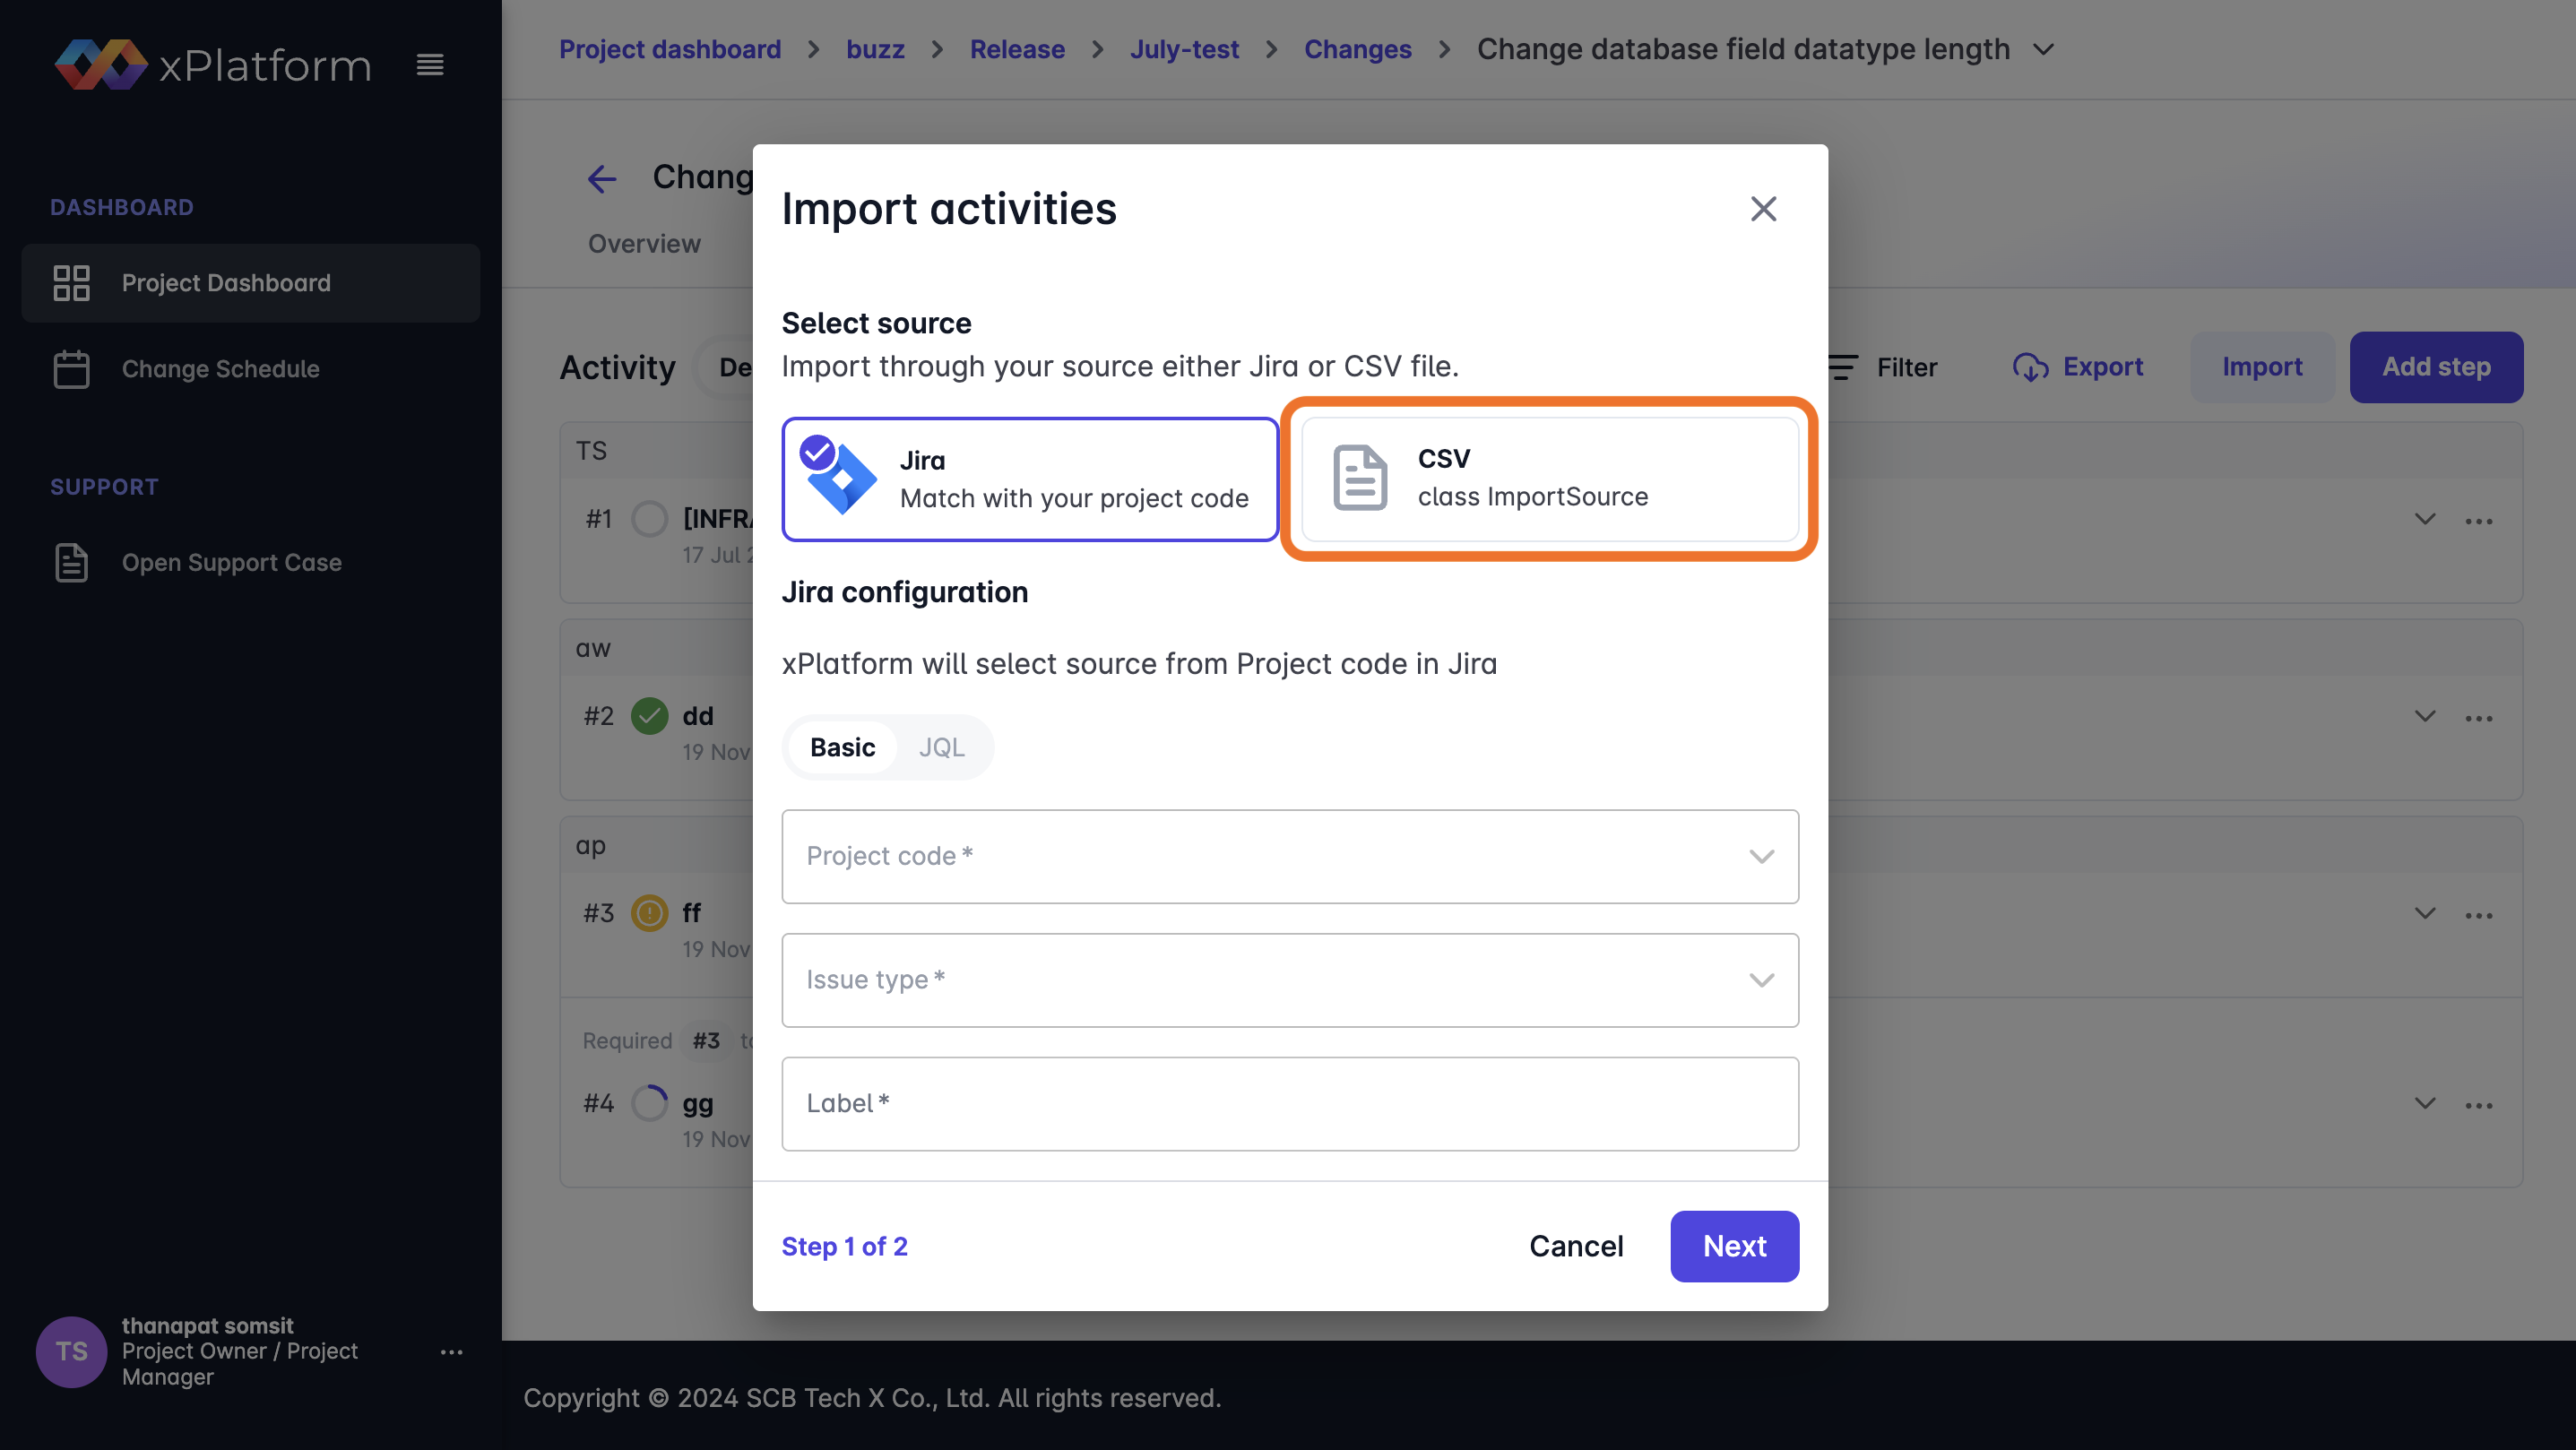
\includegraphics[width=\linewidth]{resources/pages/change-runbook/import-csv/31.png}

    \vspace{1in}

    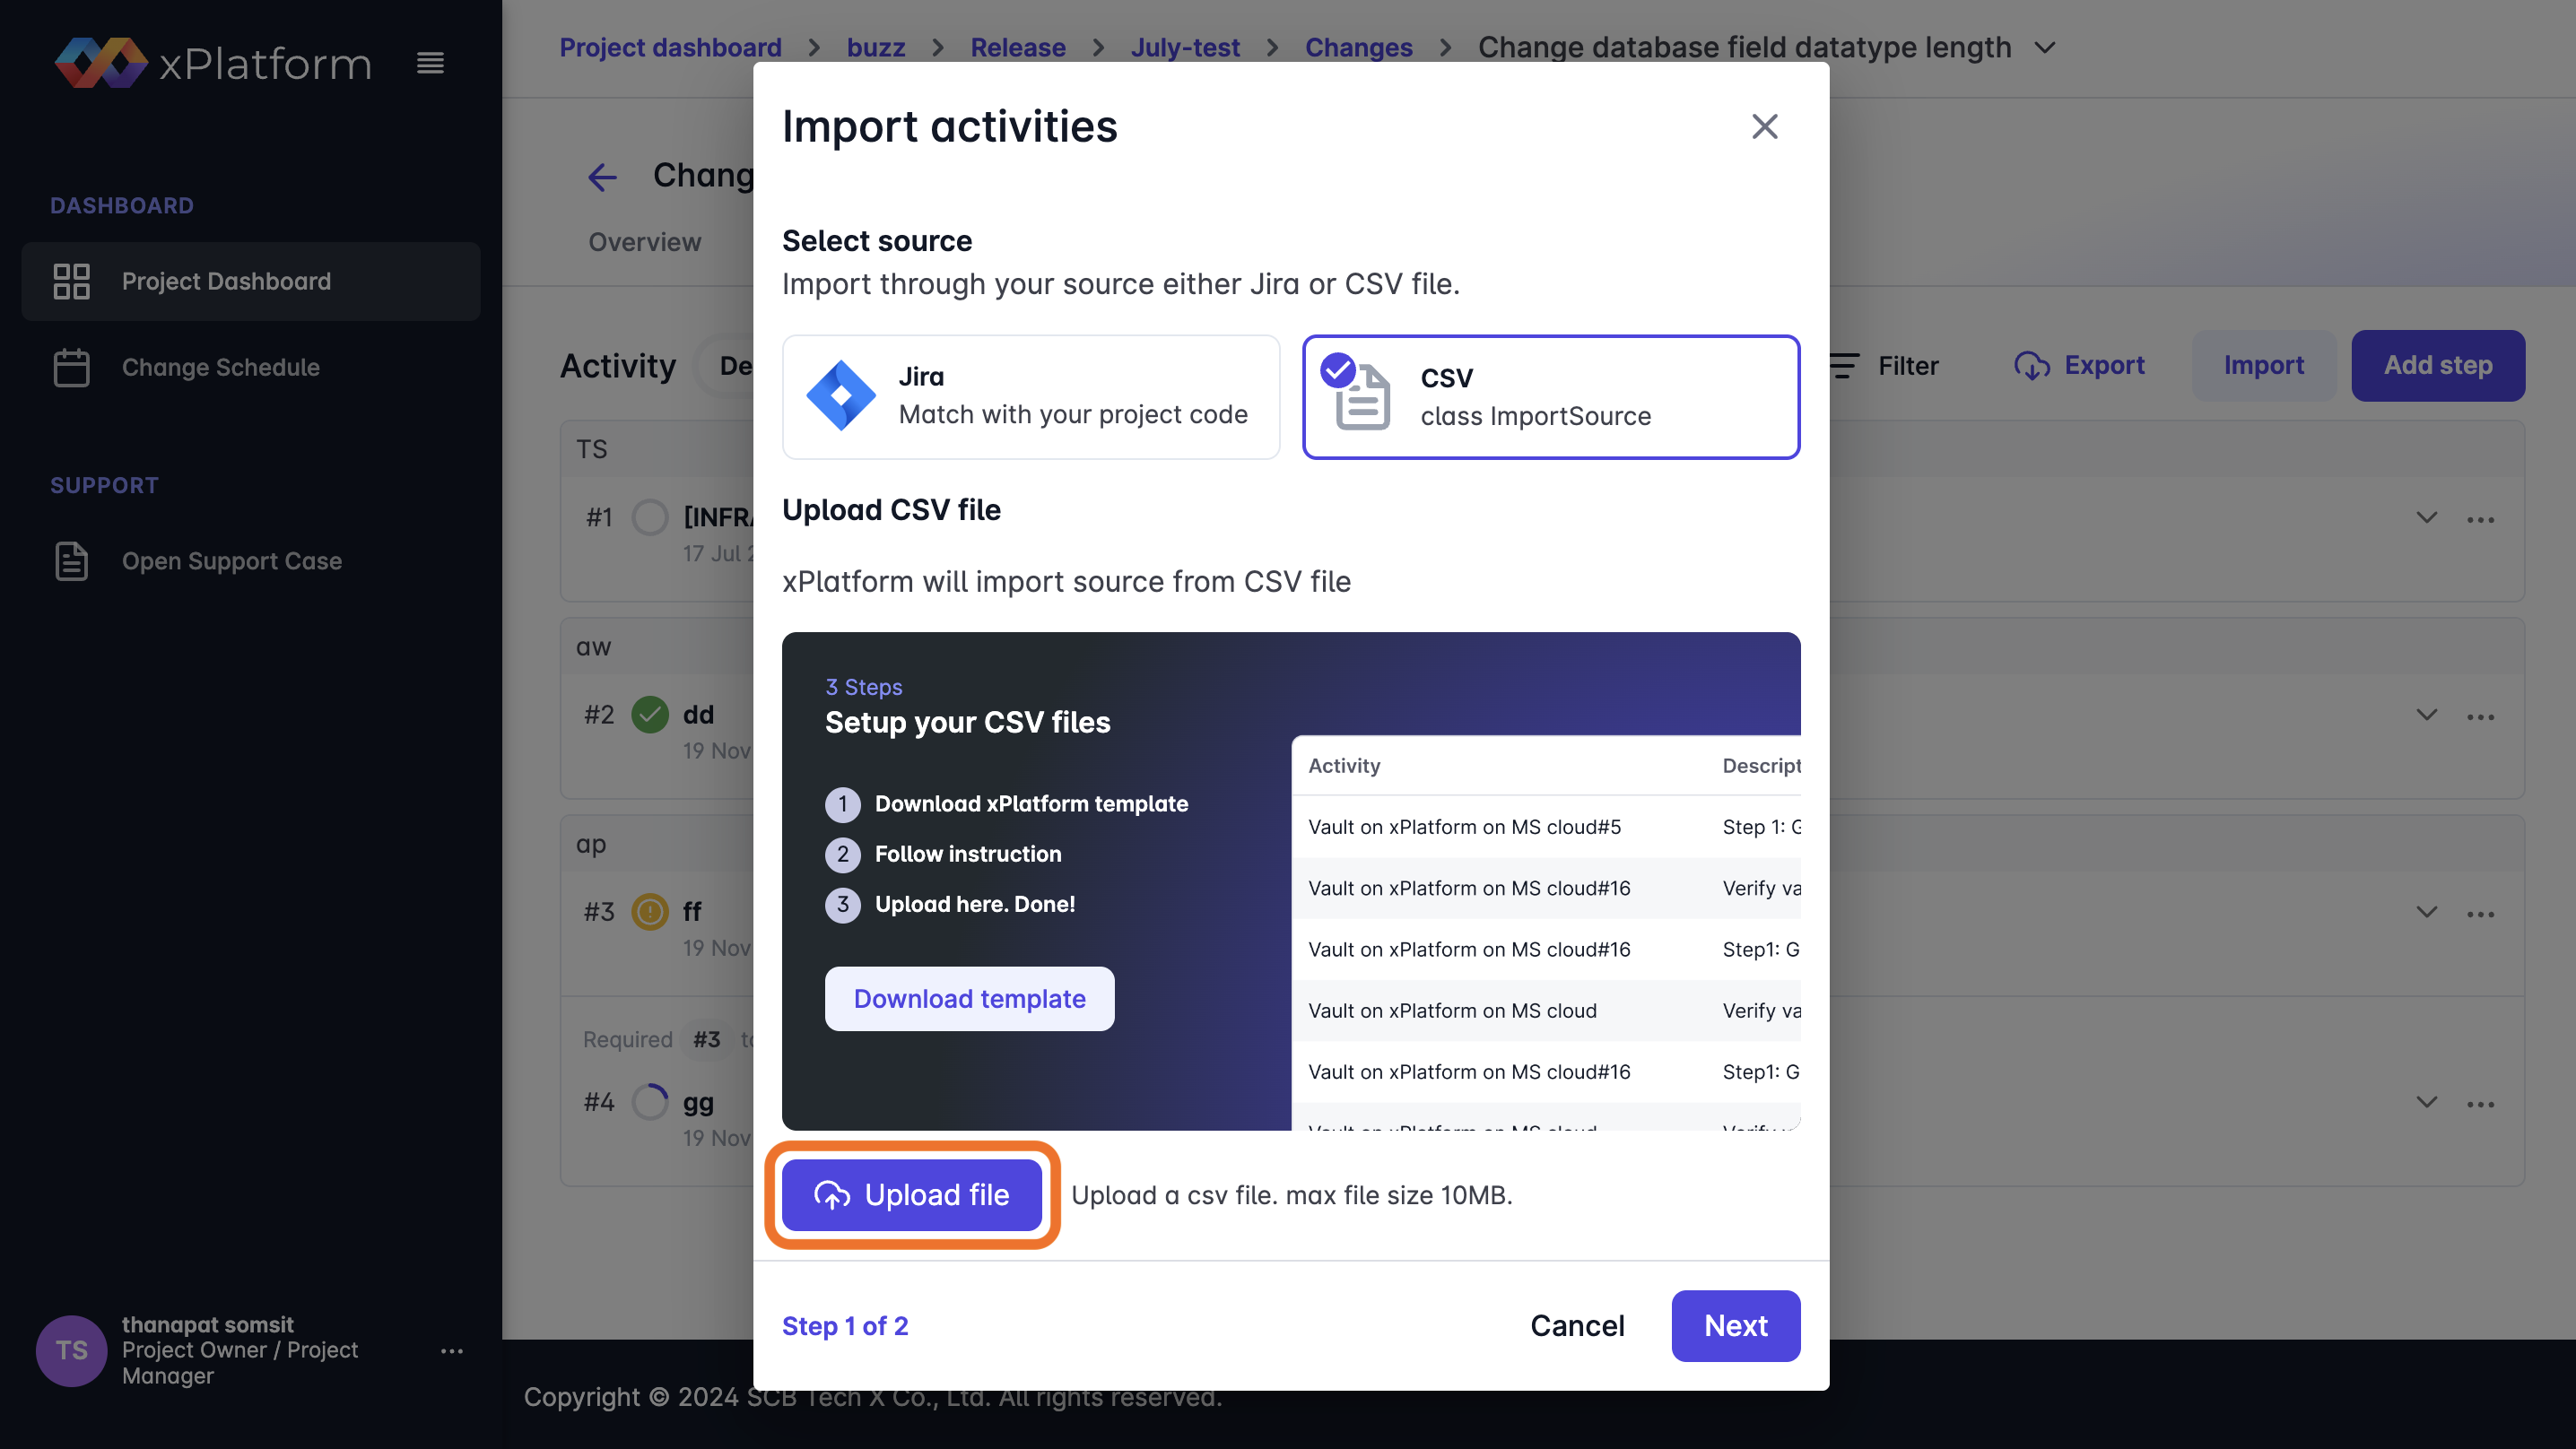
\includegraphics[width=\linewidth]{resources/pages/change-runbook/import-csv/32.png}
\end{center}
\begin{center}
    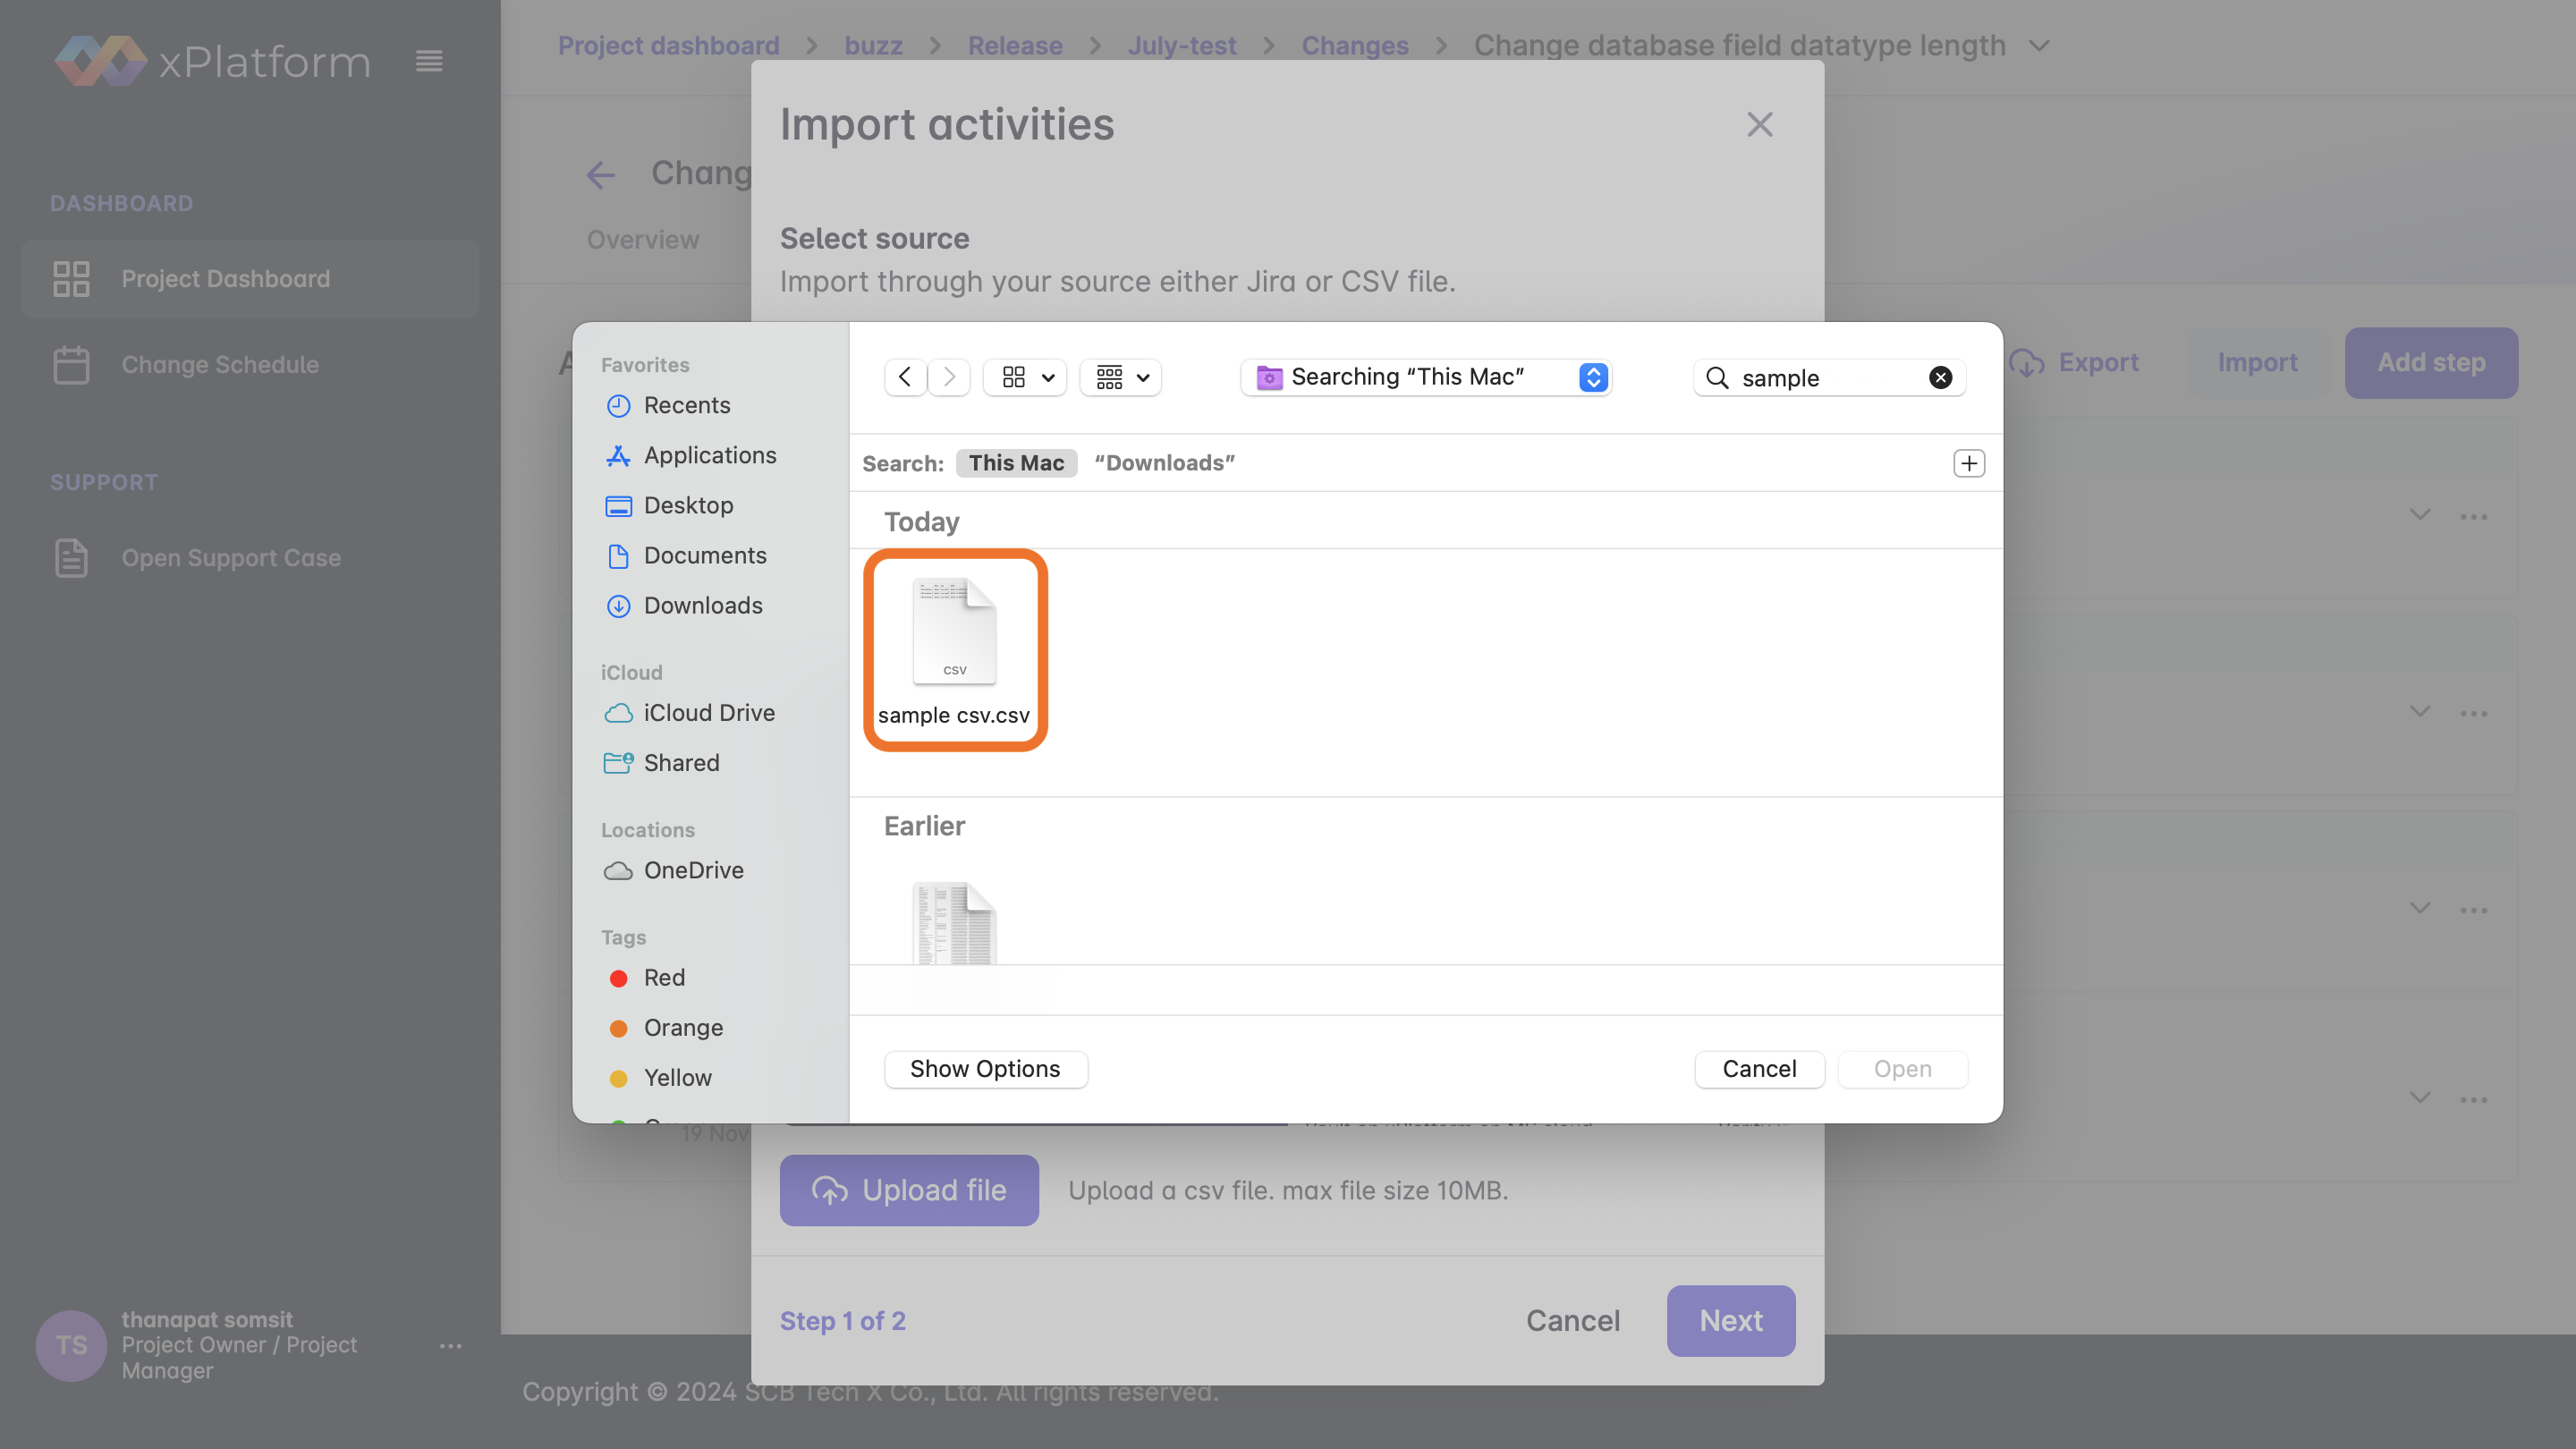
\includegraphics[width=\linewidth]{resources/pages/change-runbook/import-csv/33.png}

    \vspace{1in}

    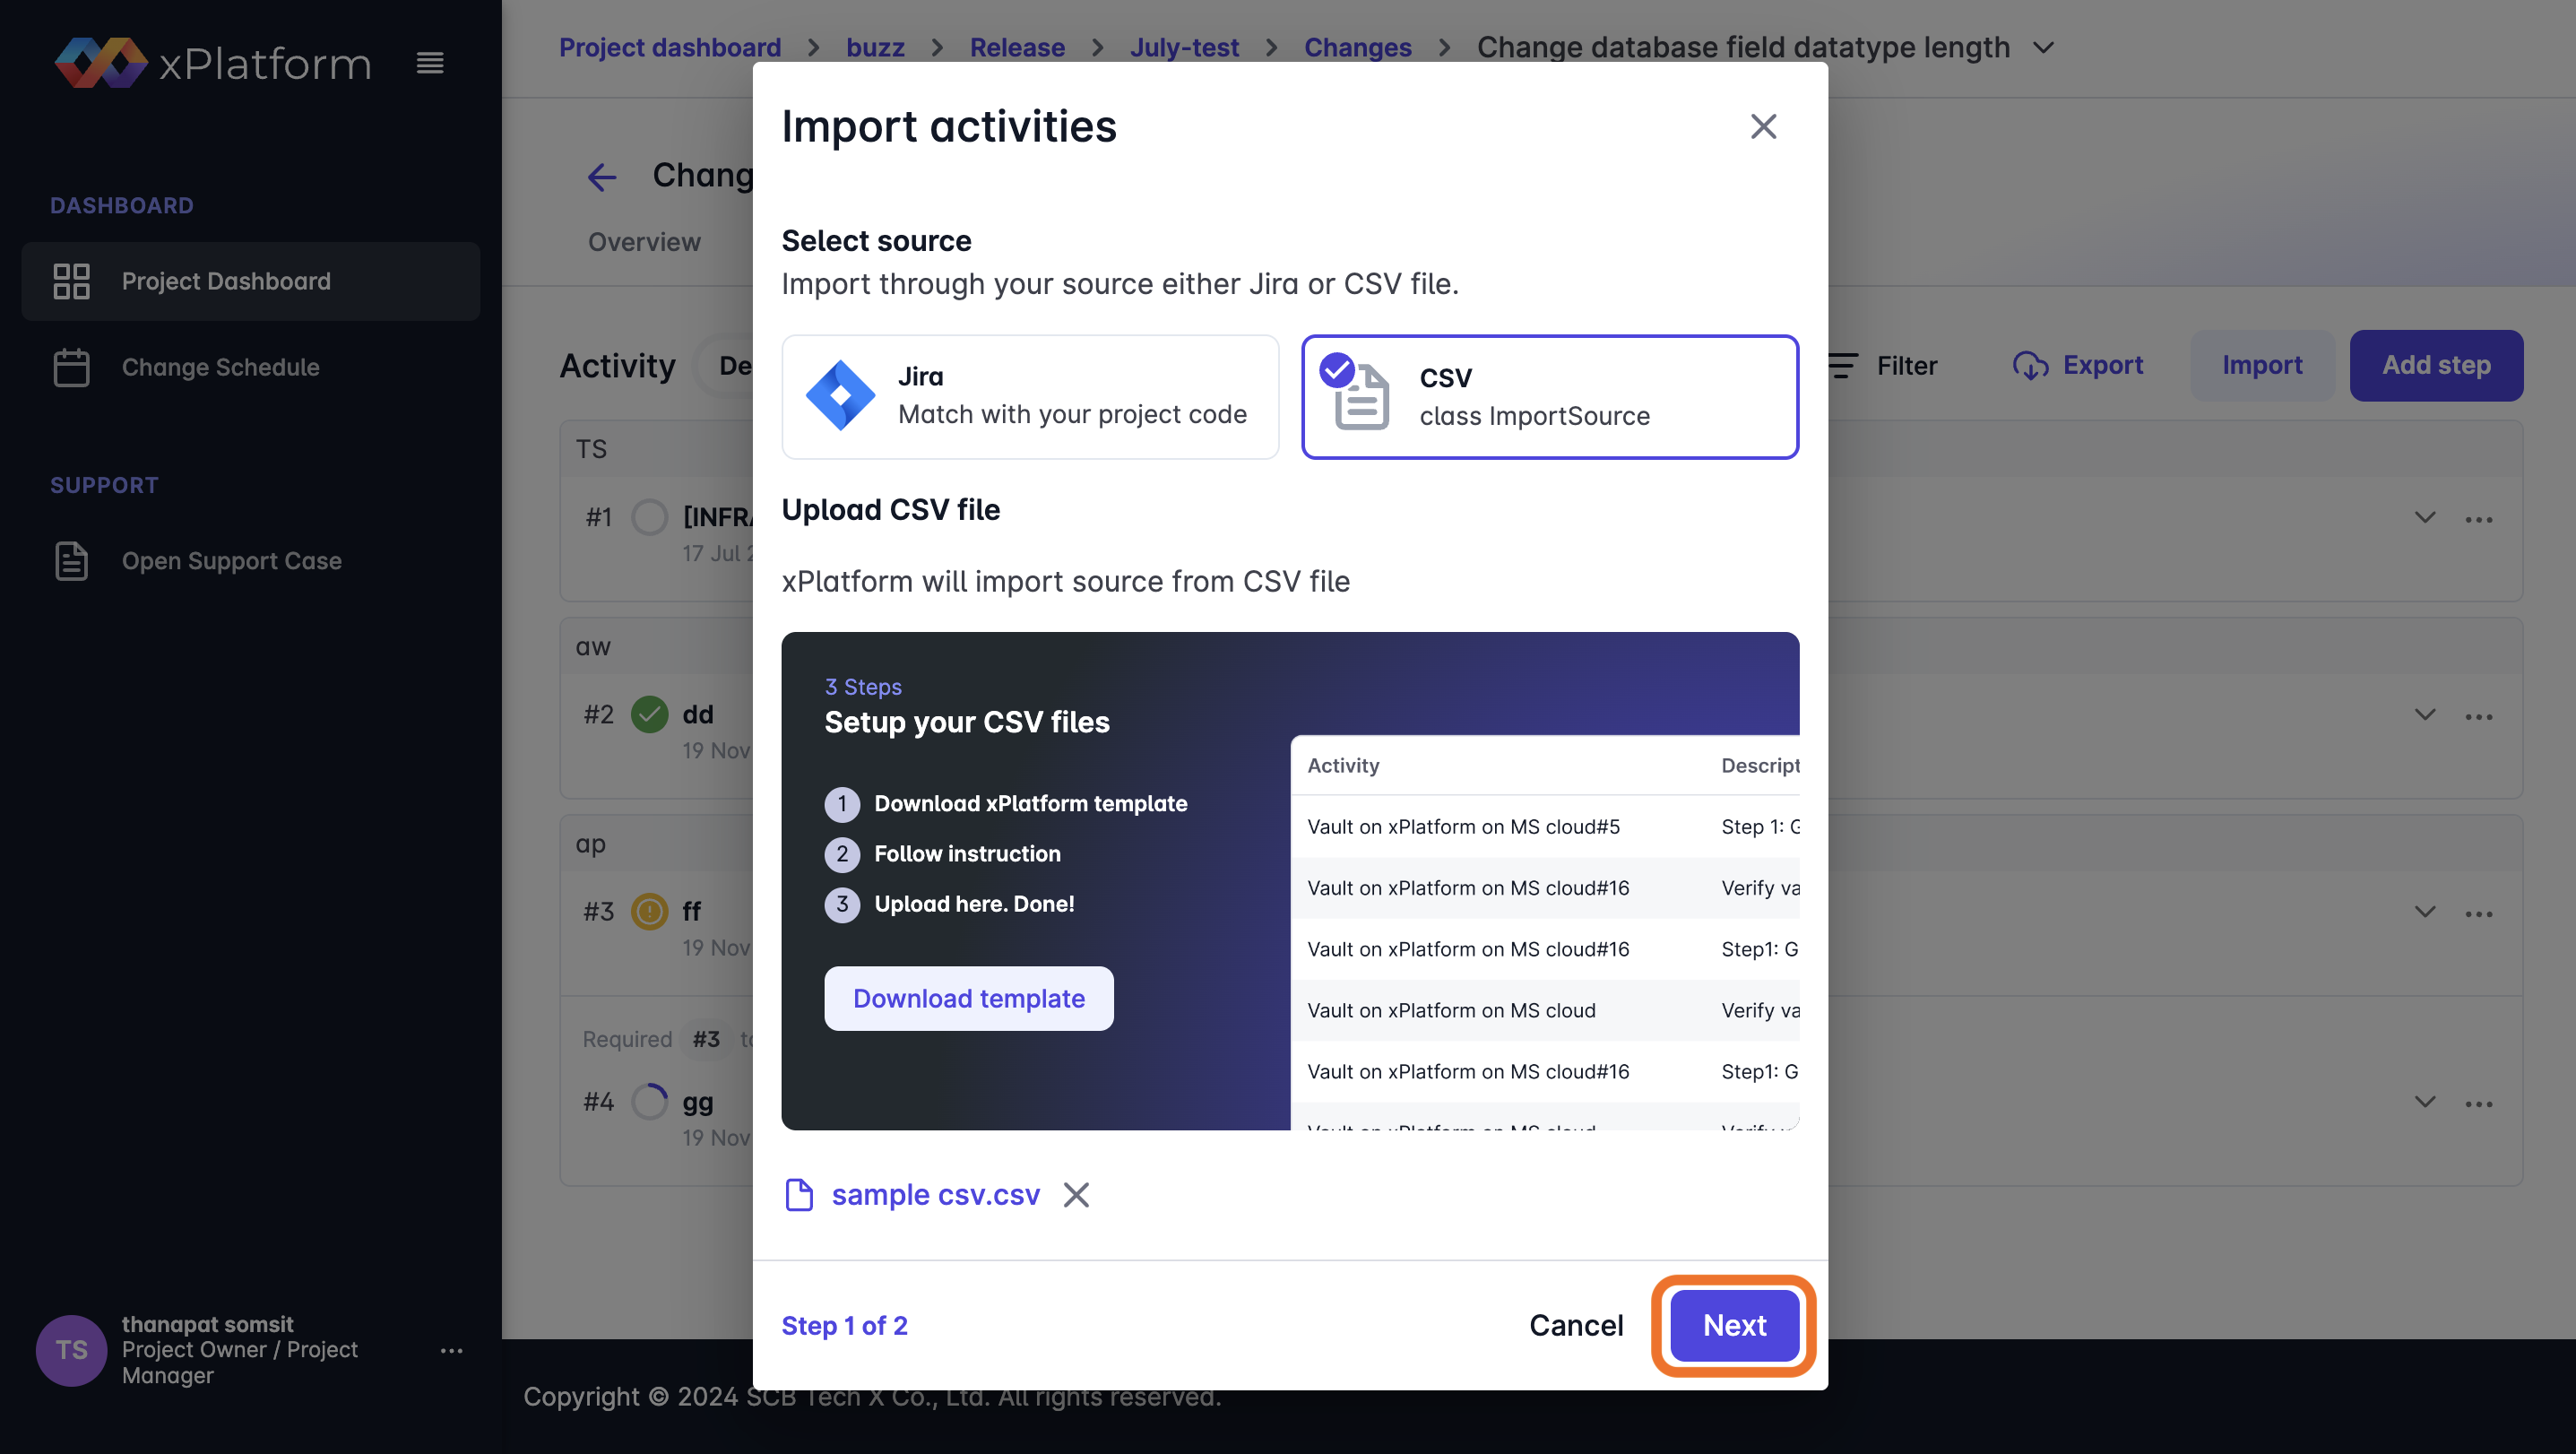
\includegraphics[width=\linewidth]{resources/pages/change-runbook/import-csv/34.png}
\end{center}
\begin{center}
    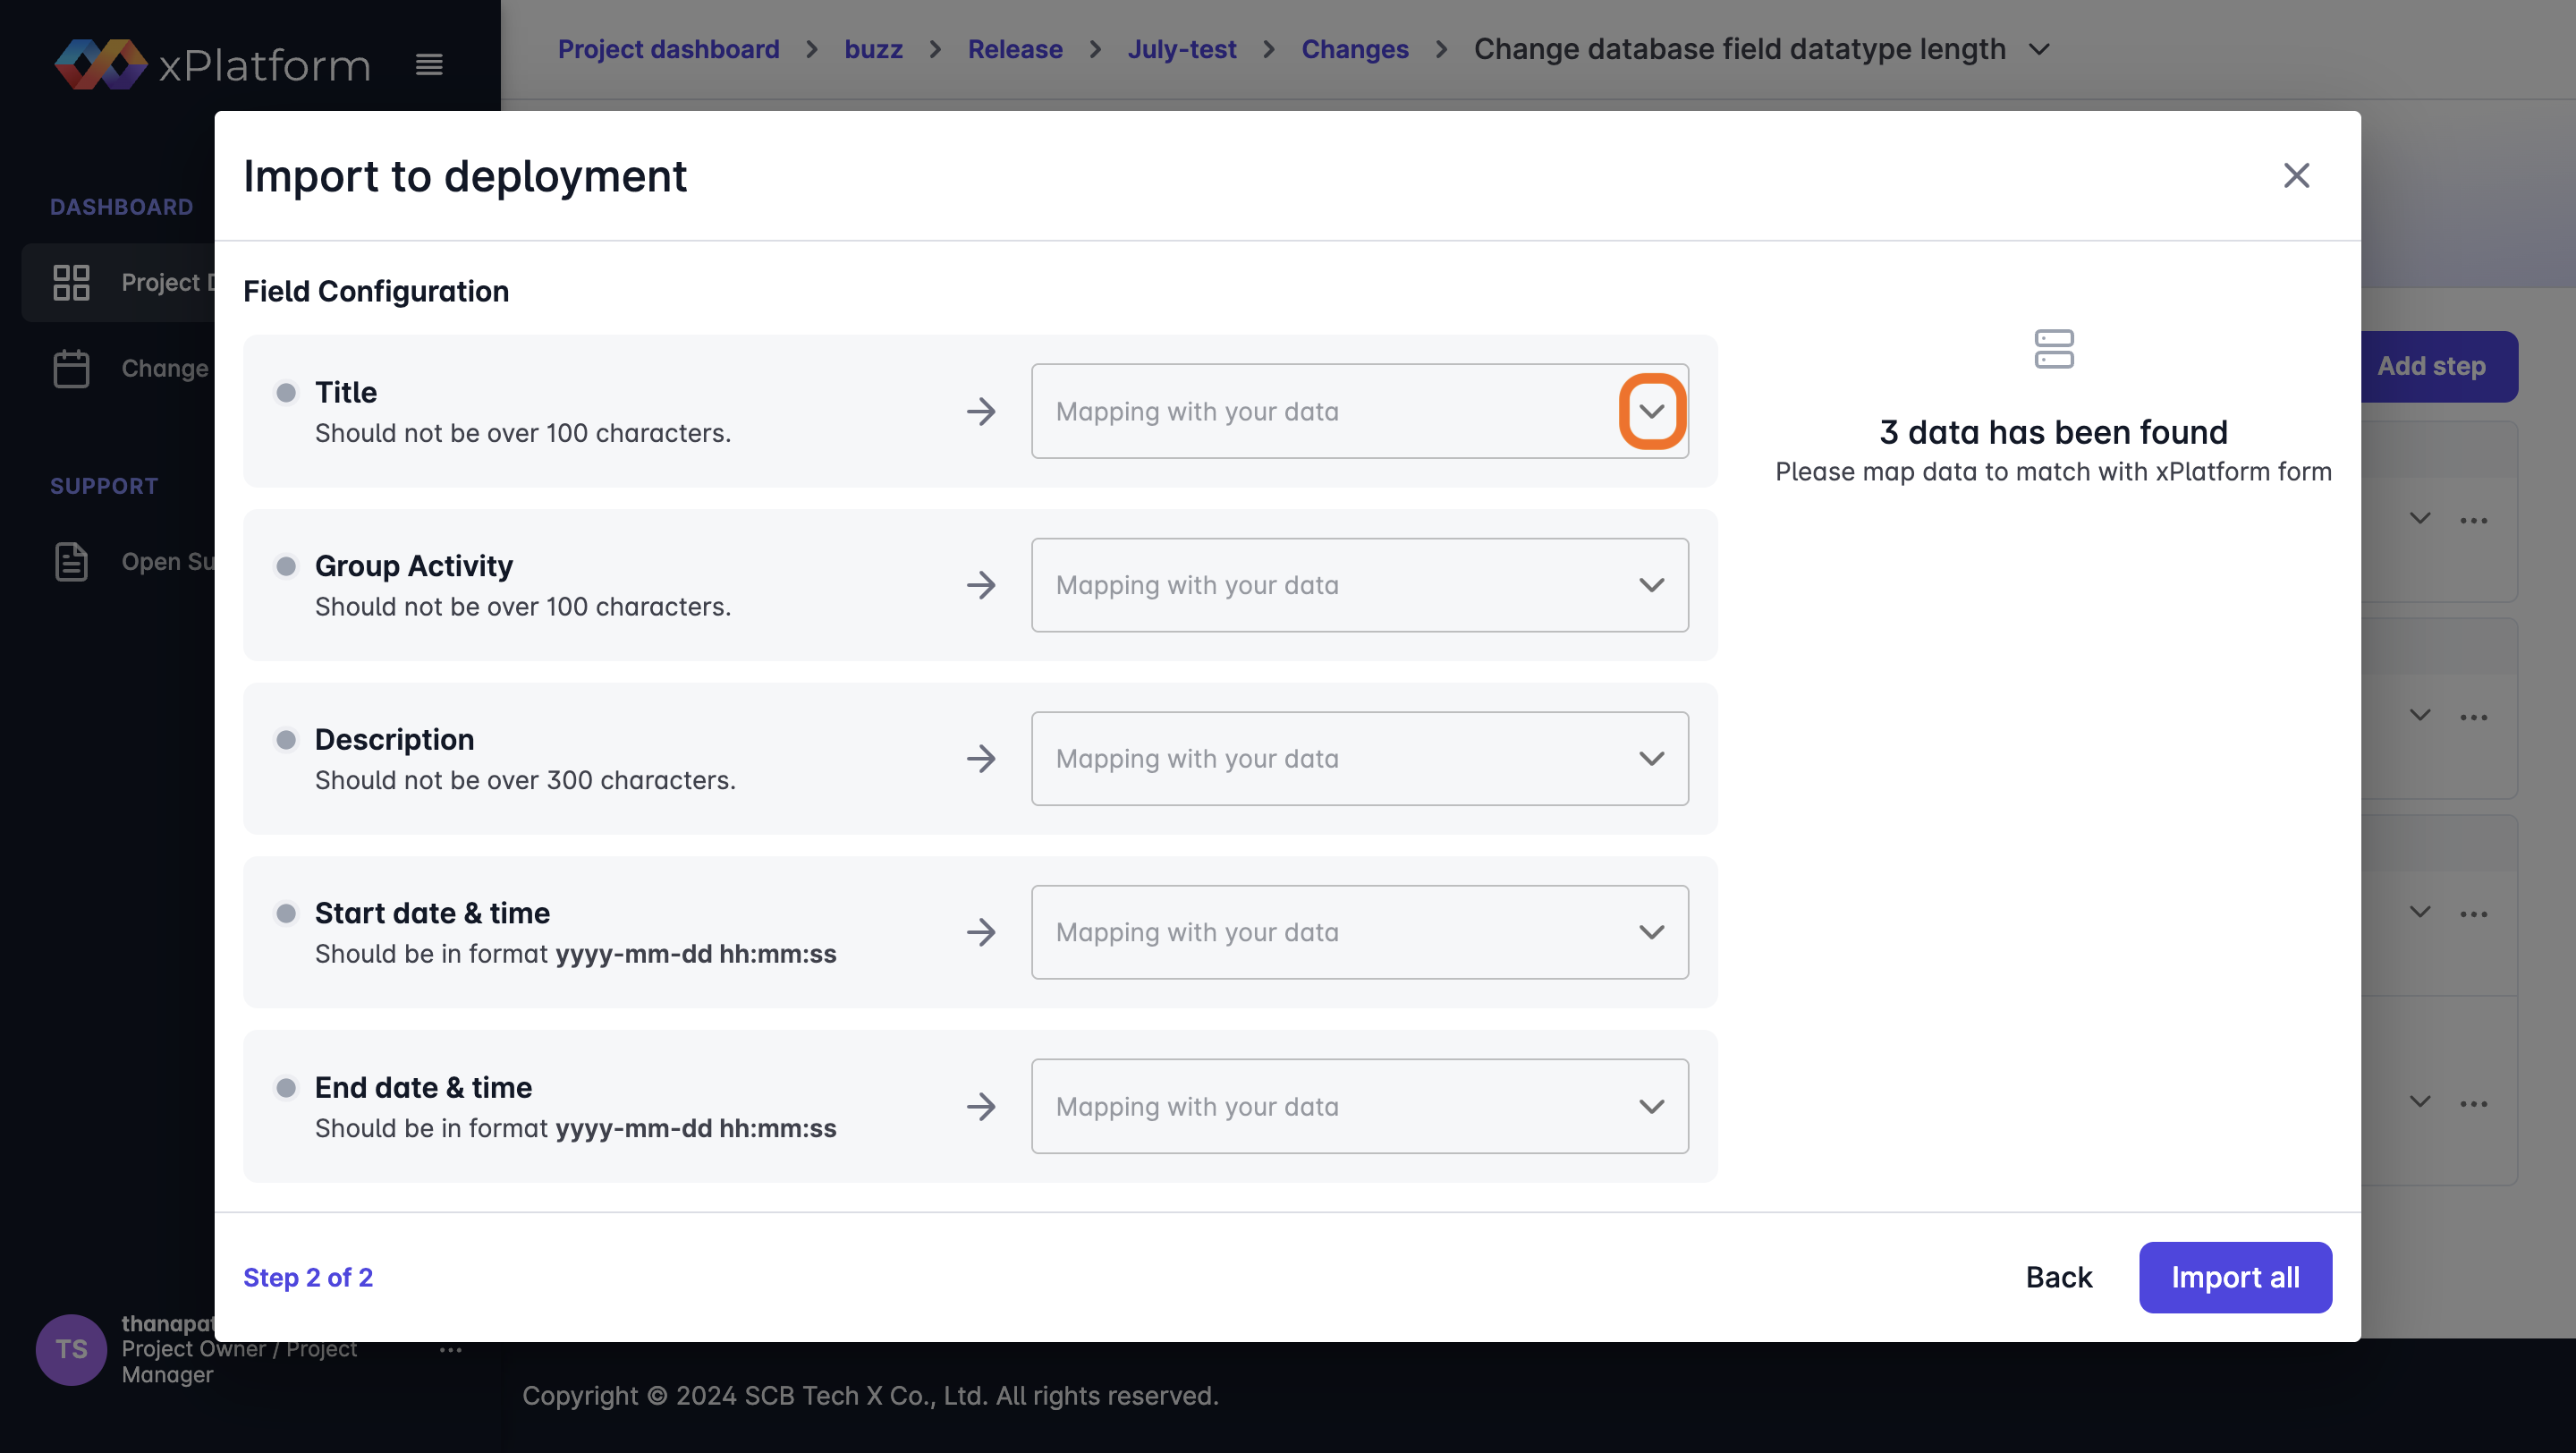
\includegraphics[width=\linewidth]{resources/pages/change-runbook/import-csv/35.png}

    \vspace{1in}

    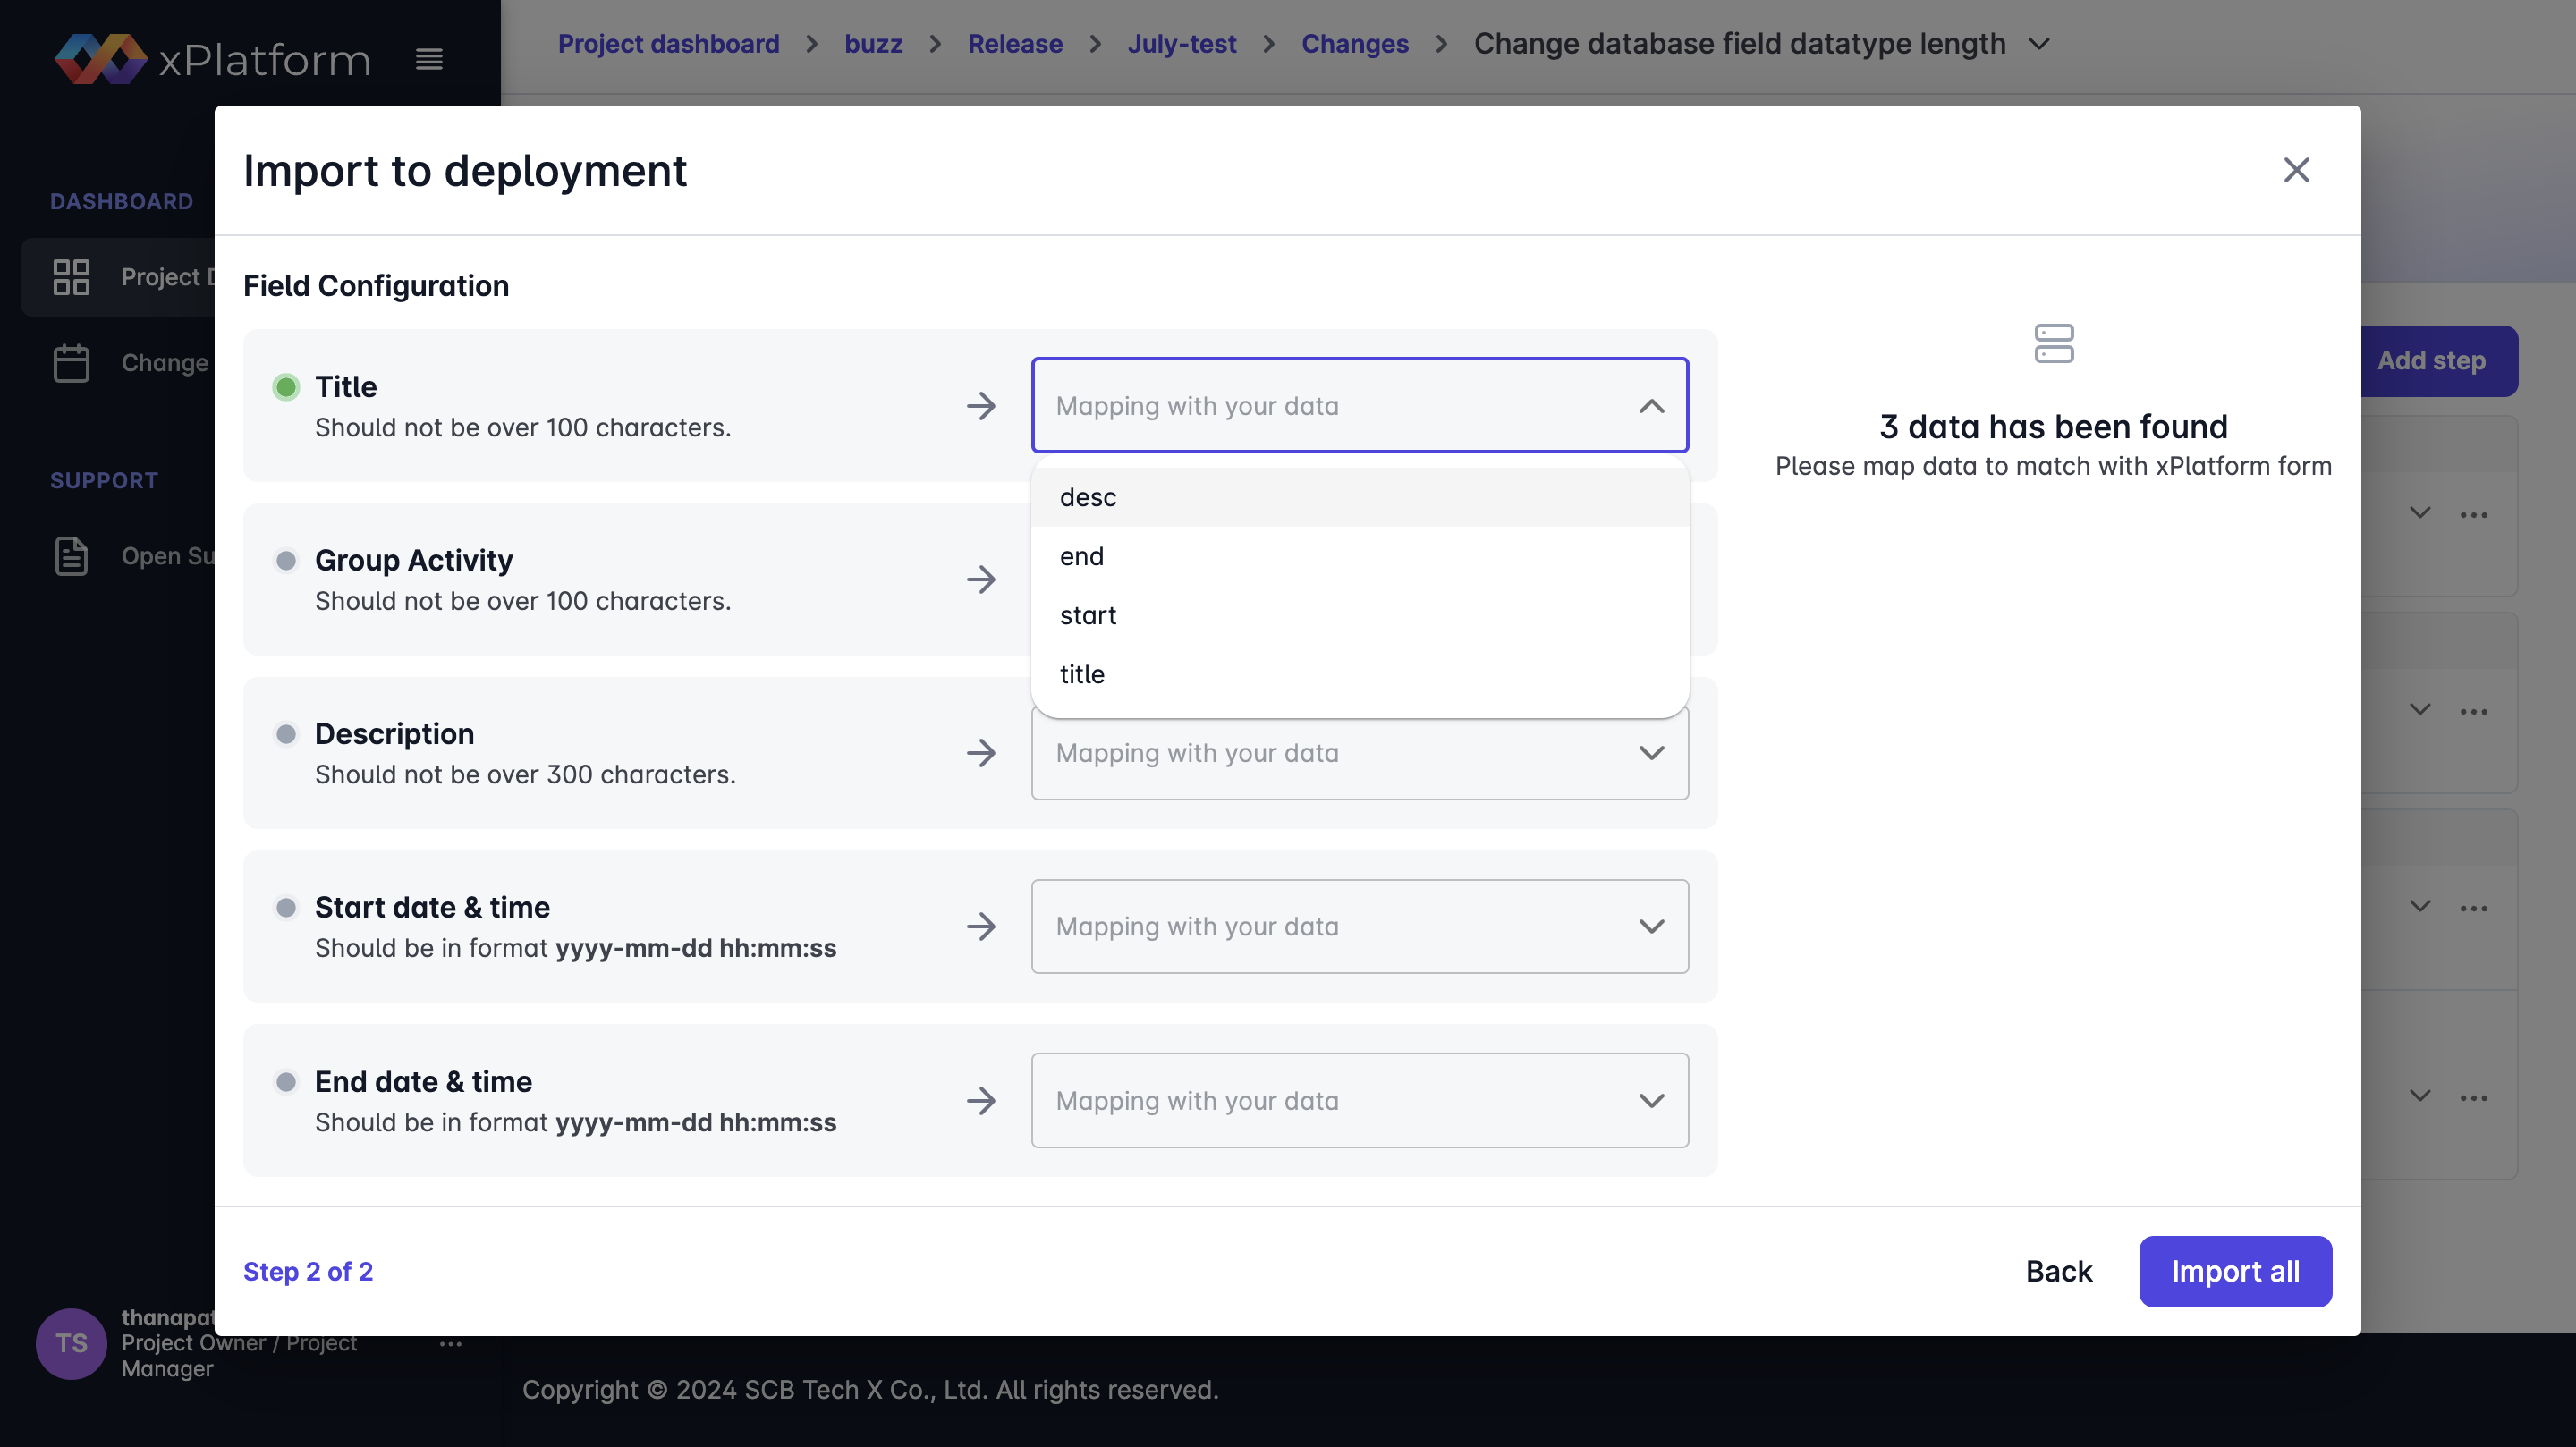
\includegraphics[width=\linewidth]{resources/pages/change-runbook/import-csv/36.png}
\end{center}

\begin{figure}[H]
    \begin{center}
        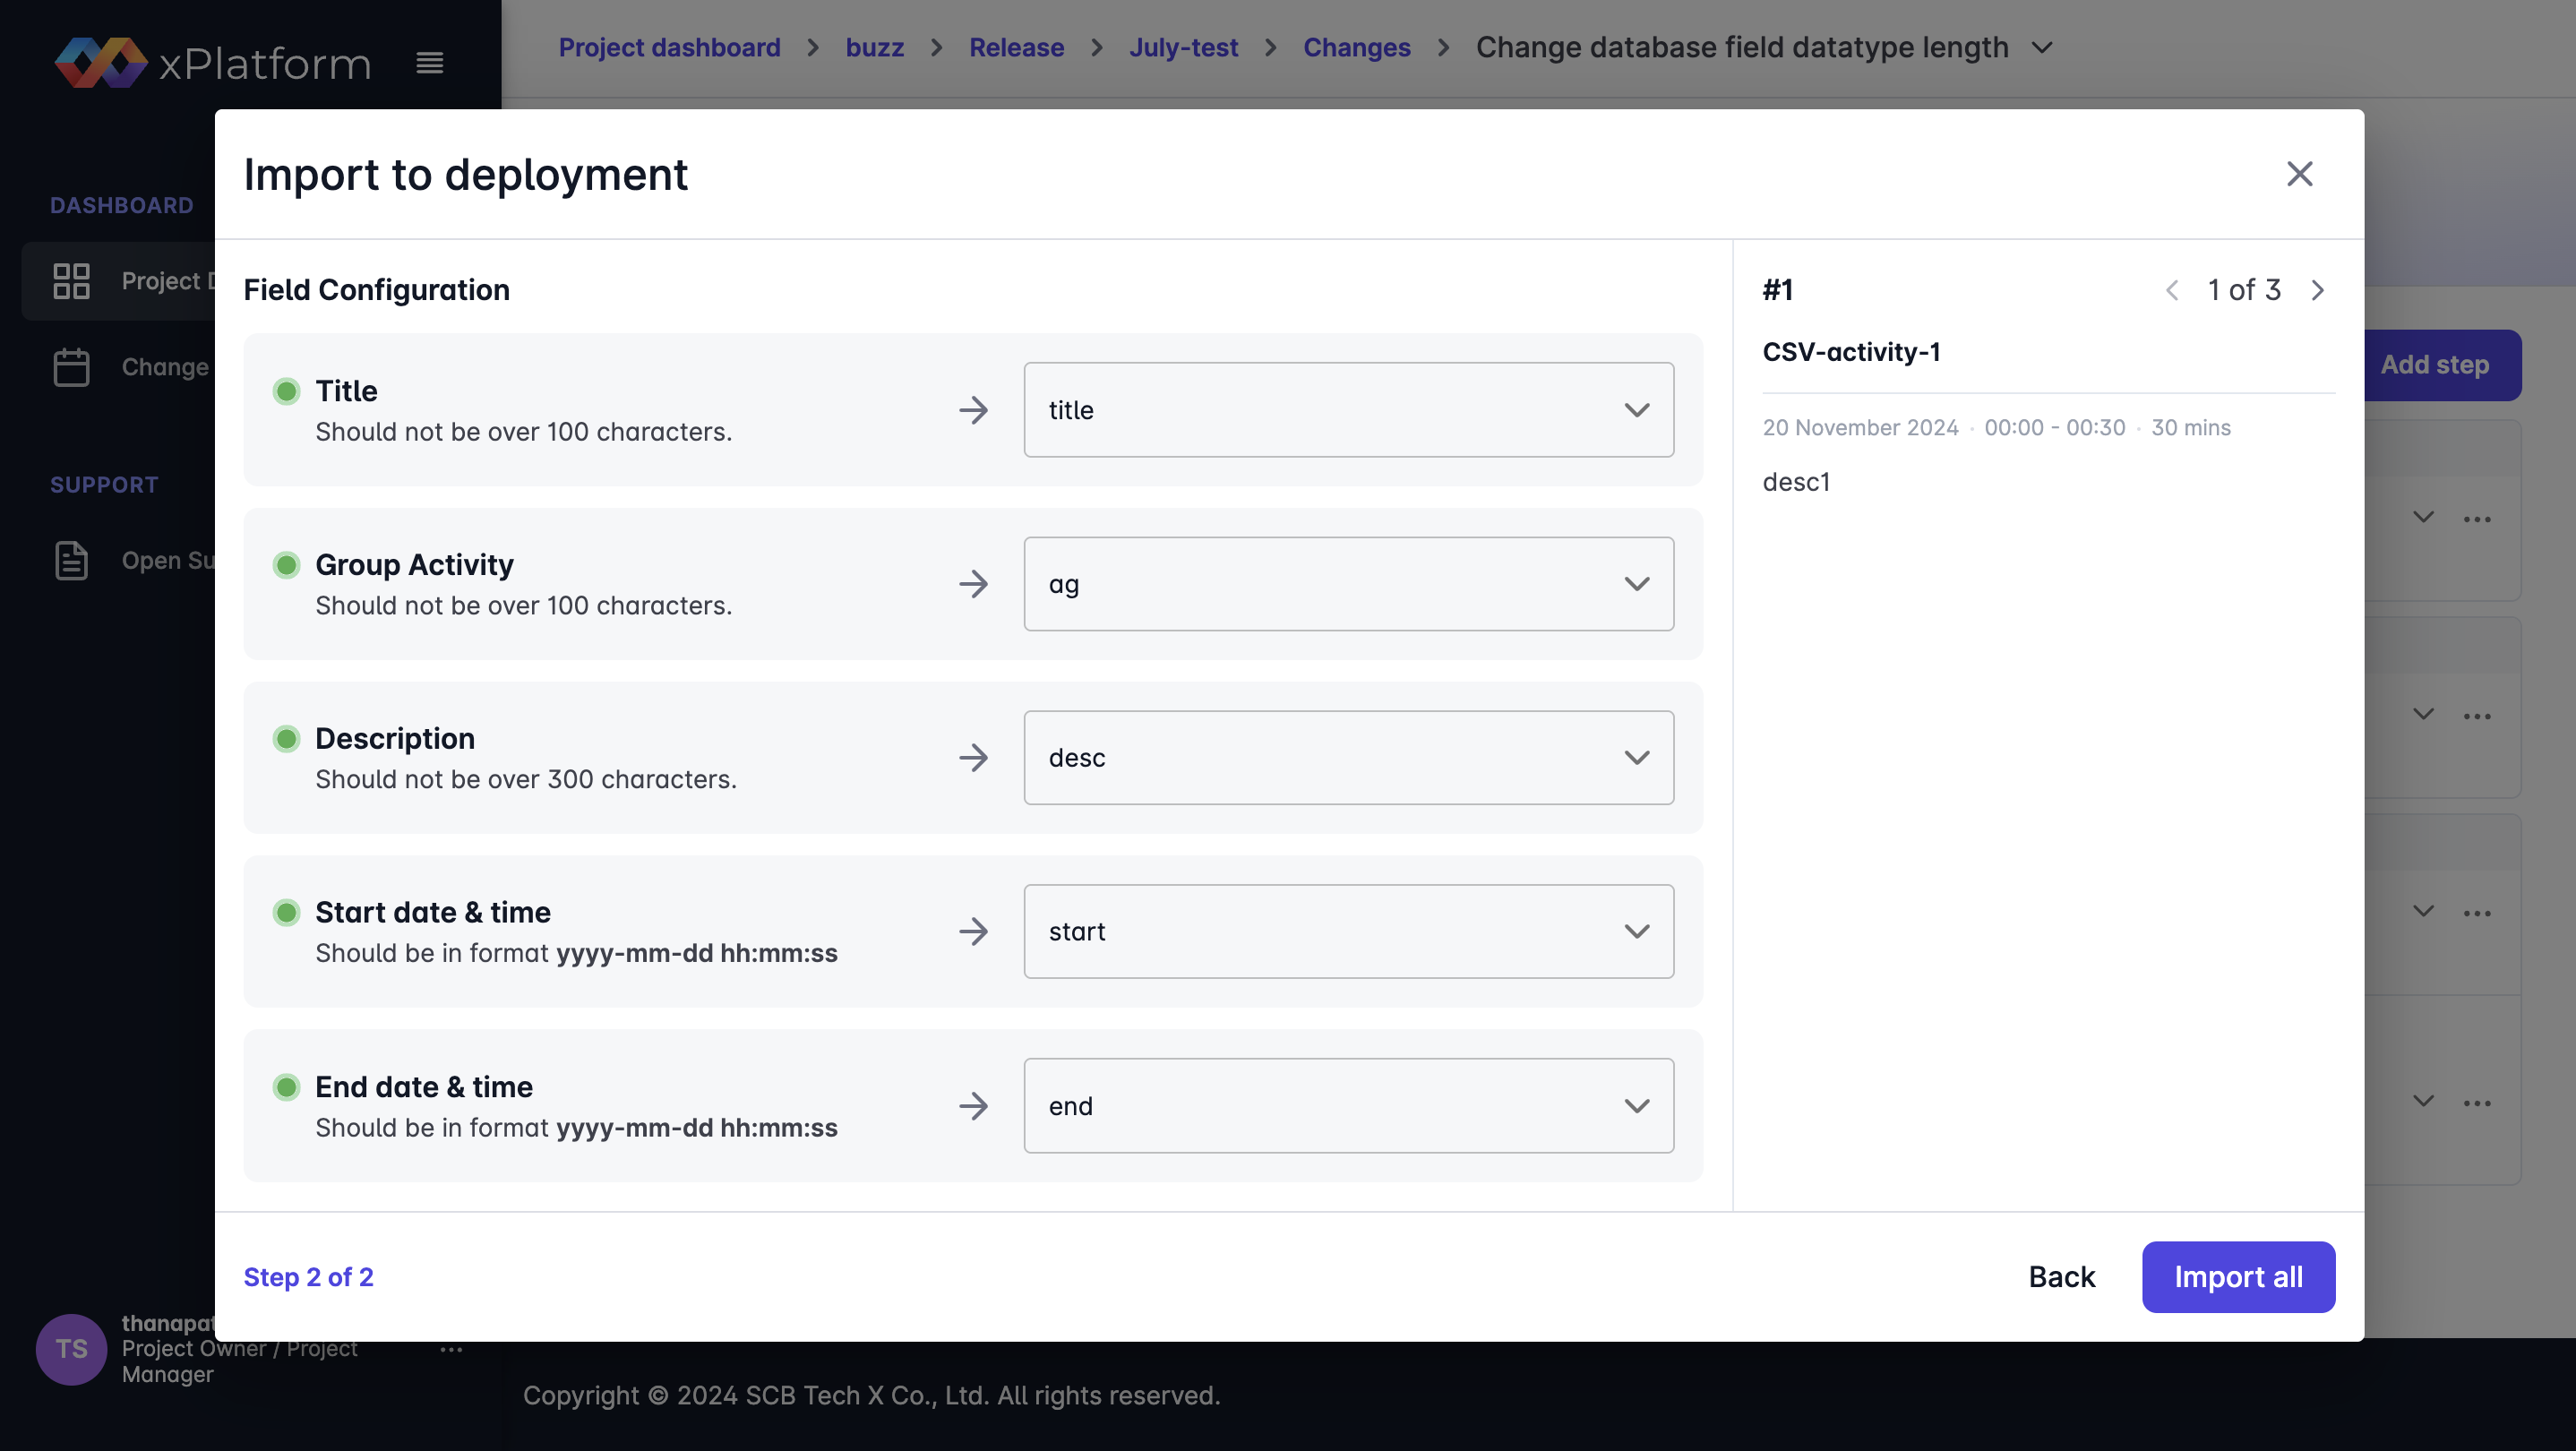
\includegraphics[width=\linewidth]{resources/pages/change-runbook/import-csv/37.png}
    
        \vspace{1in}
    
        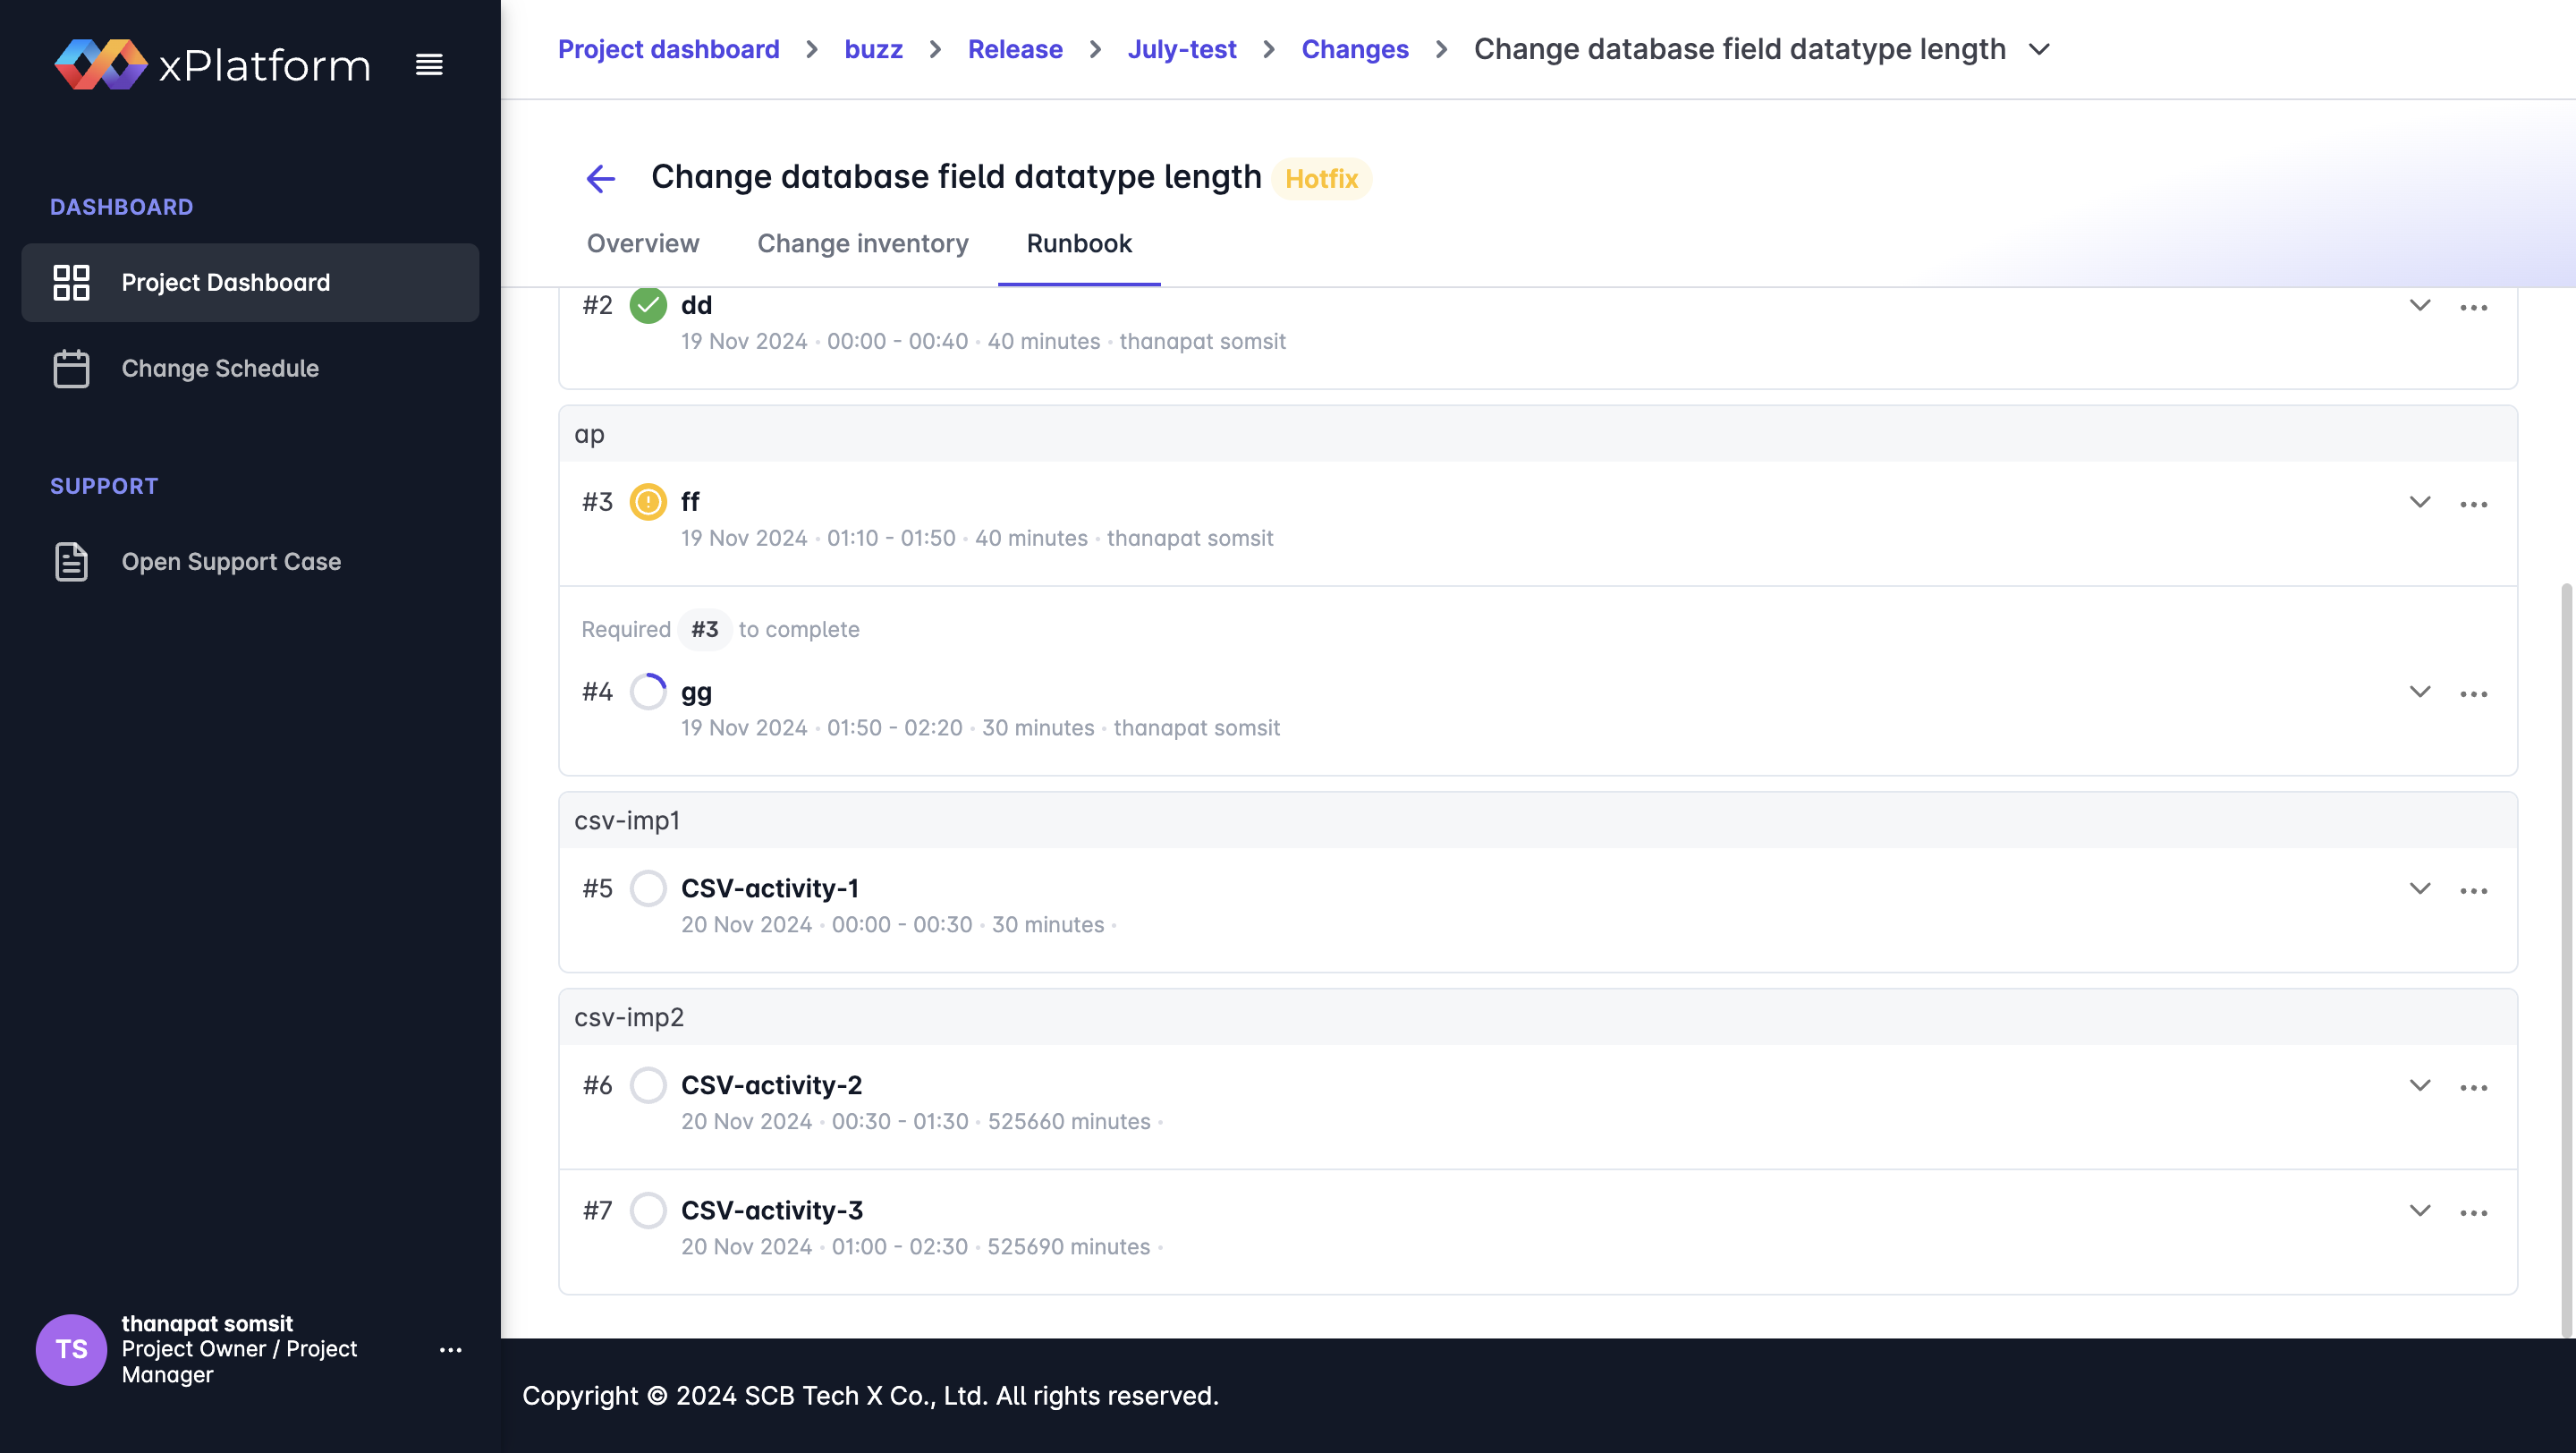
\includegraphics[width=\linewidth]{resources/pages/change-runbook/import-csv/38.png}
    \end{center}
    \caption[การดึงข้อมูลจาก CSV]{การดึงข้อมูลจาก CSV}
  \label{fig:import-csv}
\end{figure}

\newpage
\subsection{การดูข้อมูล Change Runbook ด้วย Gantt Chart}
\begin{figure}[H]
    \begin{center}
        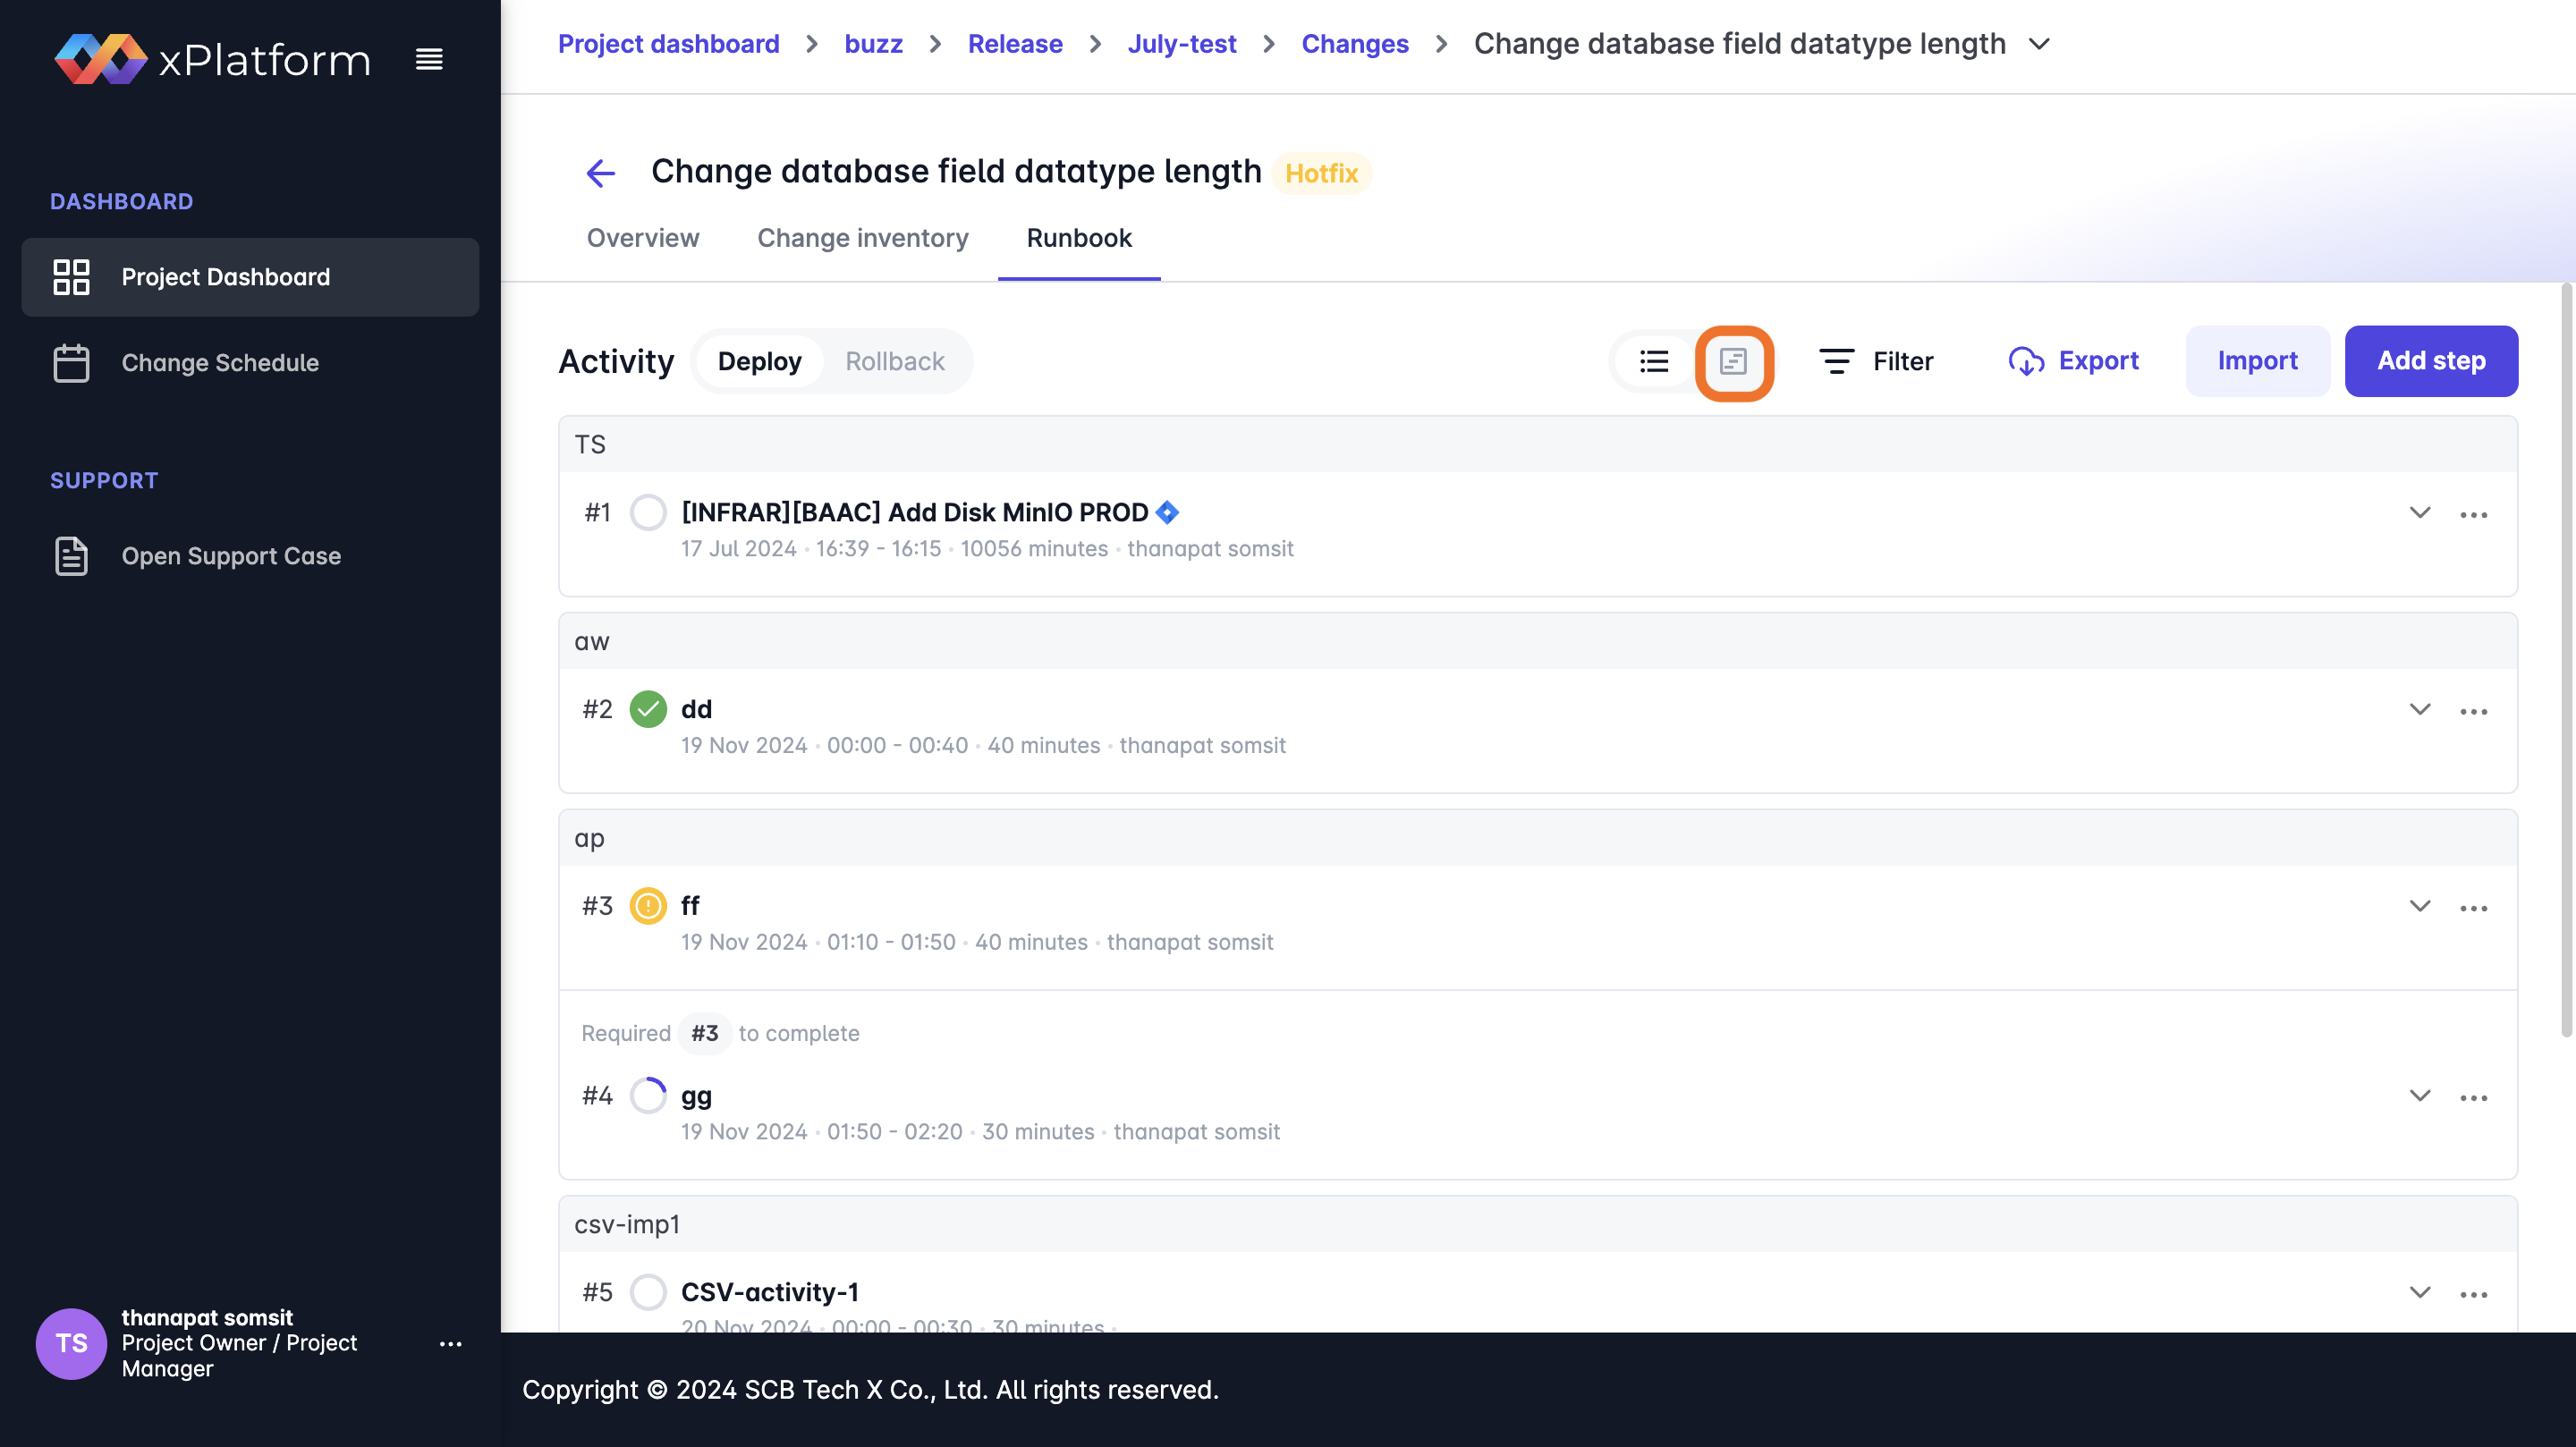
\includegraphics[width=\linewidth]{resources/pages/change-runbook/gantt-chart/39.png}
    
        \vspace{1in}
    
        \includegraphics[width=\linewidth]{resources/pages/change-runbook/gantt-chart/40.png}
    \end{center}
    \caption[Change Runbook ด้วย Gantt Chart]{Change Runbook ด้วย Gantt Chart}
  \label{fig:gantt-chart}
\end{figure}

\newpage
\subsection{การส่งออกไฟล์ Excel}
\begin{figure}[H]
    \begin{center}
        \includegraphics[width=\linewidth]{resources/pages/change-runbook/export-activity/20.png}
    
        \vspace{1in}
    
        \includegraphics[width=\linewidth]{resources/pages/change-runbook/export-activity/21.png}
    \end{center}
    \caption[การส่งออกไฟล์ Excel]{การส่งออกไฟล์ Excel}
  \label{fig:excel-export}
\end{figure}

\newpage
\section{การใช้งานฟีเจอร์ Custom Library}
\subsection{การสร้าง Custom Library Repostory}
\begin{center}
    \includegraphics[width=\linewidth]{resources/pages/custom-library/create-library/1.png}

    \vspace{1in}

    \includegraphics[width=\linewidth]{resources/pages/custom-library/create-library/2.png}
\end{center}
\begin{center}
    \includegraphics[width=\linewidth]{resources/pages/custom-library/create-library/3.png}

    \vspace{1in}

    \includegraphics[width=\linewidth]{resources/pages/custom-library/create-library/4.png}
\end{center}

\begin{figure}[H]
    \begin{center}
        \includegraphics[width=\linewidth]{resources/pages/custom-library/create-library/5.png}
    
        \vspace{1in}
    
        \includegraphics[width=\linewidth]{resources/pages/custom-library/create-library/6.png}
    \end{center}
    \caption[การสร้าง Custom Library]{การสร้าง Custom Library}
  \label{fig:create-library}
\end{figure}

\newpage
\subsection{การอัพเดตเวอร์ชัน Custom Library}
\begin{center}
    \includegraphics[width=\linewidth]{resources/pages/custom-library/update-library/6.png}

    \vspace{1in}

    \includegraphics[width=\linewidth]{resources/pages/custom-library/update-library/7.png}
\end{center}

\begin{figure}[H]
    \begin{center}
        \includegraphics[width=\linewidth]{resources/pages/custom-library/update-library/8.png}
    
        \vspace{1in}
    
        \includegraphics[width=\linewidth]{resources/pages/custom-library/update-library/9.png}
    \end{center}
    \caption[การอัพเดตเวอร์ชัน Custom Library]{การอัพเดตเวอร์ชัน Custom Library}
  \label{fig:update-library}
\end{figure}


\newpage
\section{การใช้งานฟีเจอร์ Documentation}
\begin{center}
    \includegraphics[width=\linewidth]{resources/pages/documentation/1.png}

    \vspace{1in}

    \includegraphics[width=\linewidth]{resources/pages/documentation/2.png}
\end{center}

\begin{figure}[H]
    \begin{center}
        \includegraphics[width=\linewidth]{resources/pages/documentation/3.png}
    \end{center}
    \caption[การใช้งานฟีเจอร์ Documentation]{การใช้งานฟีเจอร์ Documentation}
  \label{fig:documentation}
\end{figure}

%% Display glossary (optional) -- need glossary option.
% \ifglossary\glossarypage\fi

%% Display index (optional) -- need idx option.
% \ifindex\indexpage\fi

% \begin{biosketch}
% \begin{center}
%   \includegraphics[width=1.5in]{mugshot.jpg}
% \end{center}
% Your biosketch goes here. Make sure it sits inside
% the \texttt{biosketch} environment.
% \end{biosketch}
% \fi % \ifproject
\end{document}
